% Options for packages loaded elsewhere
\PassOptionsToPackage{unicode}{hyperref}
\PassOptionsToPackage{hyphens}{url}
\PassOptionsToPackage{dvipsnames,svgnames,x11names}{xcolor}
%
\documentclass[
  letterpaper,
  DIV=11,
  numbers=noendperiod]{scrreprt}

\usepackage{amsmath,amssymb}
\usepackage{iftex}
\ifPDFTeX
  \usepackage[T1]{fontenc}
  \usepackage[utf8]{inputenc}
  \usepackage{textcomp} % provide euro and other symbols
\else % if luatex or xetex
  \usepackage{unicode-math}
  \defaultfontfeatures{Scale=MatchLowercase}
  \defaultfontfeatures[\rmfamily]{Ligatures=TeX,Scale=1}
\fi
\usepackage{lmodern}
\ifPDFTeX\else  
    % xetex/luatex font selection
\fi
% Use upquote if available, for straight quotes in verbatim environments
\IfFileExists{upquote.sty}{\usepackage{upquote}}{}
\IfFileExists{microtype.sty}{% use microtype if available
  \usepackage[]{microtype}
  \UseMicrotypeSet[protrusion]{basicmath} % disable protrusion for tt fonts
}{}
\makeatletter
\@ifundefined{KOMAClassName}{% if non-KOMA class
  \IfFileExists{parskip.sty}{%
    \usepackage{parskip}
  }{% else
    \setlength{\parindent}{0pt}
    \setlength{\parskip}{6pt plus 2pt minus 1pt}}
}{% if KOMA class
  \KOMAoptions{parskip=half}}
\makeatother
\usepackage{xcolor}
\setlength{\emergencystretch}{3em} % prevent overfull lines
\setcounter{secnumdepth}{5}
% Make \paragraph and \subparagraph free-standing
\ifx\paragraph\undefined\else
  \let\oldparagraph\paragraph
  \renewcommand{\paragraph}[1]{\oldparagraph{#1}\mbox{}}
\fi
\ifx\subparagraph\undefined\else
  \let\oldsubparagraph\subparagraph
  \renewcommand{\subparagraph}[1]{\oldsubparagraph{#1}\mbox{}}
\fi

\usepackage{color}
\usepackage{fancyvrb}
\newcommand{\VerbBar}{|}
\newcommand{\VERB}{\Verb[commandchars=\\\{\}]}
\DefineVerbatimEnvironment{Highlighting}{Verbatim}{commandchars=\\\{\}}
% Add ',fontsize=\small' for more characters per line
\usepackage{framed}
\definecolor{shadecolor}{RGB}{241,243,245}
\newenvironment{Shaded}{\begin{snugshade}}{\end{snugshade}}
\newcommand{\AlertTok}[1]{\textcolor[rgb]{0.68,0.00,0.00}{#1}}
\newcommand{\AnnotationTok}[1]{\textcolor[rgb]{0.37,0.37,0.37}{#1}}
\newcommand{\AttributeTok}[1]{\textcolor[rgb]{0.40,0.45,0.13}{#1}}
\newcommand{\BaseNTok}[1]{\textcolor[rgb]{0.68,0.00,0.00}{#1}}
\newcommand{\BuiltInTok}[1]{\textcolor[rgb]{0.00,0.23,0.31}{#1}}
\newcommand{\CharTok}[1]{\textcolor[rgb]{0.13,0.47,0.30}{#1}}
\newcommand{\CommentTok}[1]{\textcolor[rgb]{0.37,0.37,0.37}{#1}}
\newcommand{\CommentVarTok}[1]{\textcolor[rgb]{0.37,0.37,0.37}{\textit{#1}}}
\newcommand{\ConstantTok}[1]{\textcolor[rgb]{0.56,0.35,0.01}{#1}}
\newcommand{\ControlFlowTok}[1]{\textcolor[rgb]{0.00,0.23,0.31}{#1}}
\newcommand{\DataTypeTok}[1]{\textcolor[rgb]{0.68,0.00,0.00}{#1}}
\newcommand{\DecValTok}[1]{\textcolor[rgb]{0.68,0.00,0.00}{#1}}
\newcommand{\DocumentationTok}[1]{\textcolor[rgb]{0.37,0.37,0.37}{\textit{#1}}}
\newcommand{\ErrorTok}[1]{\textcolor[rgb]{0.68,0.00,0.00}{#1}}
\newcommand{\ExtensionTok}[1]{\textcolor[rgb]{0.00,0.23,0.31}{#1}}
\newcommand{\FloatTok}[1]{\textcolor[rgb]{0.68,0.00,0.00}{#1}}
\newcommand{\FunctionTok}[1]{\textcolor[rgb]{0.28,0.35,0.67}{#1}}
\newcommand{\ImportTok}[1]{\textcolor[rgb]{0.00,0.46,0.62}{#1}}
\newcommand{\InformationTok}[1]{\textcolor[rgb]{0.37,0.37,0.37}{#1}}
\newcommand{\KeywordTok}[1]{\textcolor[rgb]{0.00,0.23,0.31}{#1}}
\newcommand{\NormalTok}[1]{\textcolor[rgb]{0.00,0.23,0.31}{#1}}
\newcommand{\OperatorTok}[1]{\textcolor[rgb]{0.37,0.37,0.37}{#1}}
\newcommand{\OtherTok}[1]{\textcolor[rgb]{0.00,0.23,0.31}{#1}}
\newcommand{\PreprocessorTok}[1]{\textcolor[rgb]{0.68,0.00,0.00}{#1}}
\newcommand{\RegionMarkerTok}[1]{\textcolor[rgb]{0.00,0.23,0.31}{#1}}
\newcommand{\SpecialCharTok}[1]{\textcolor[rgb]{0.37,0.37,0.37}{#1}}
\newcommand{\SpecialStringTok}[1]{\textcolor[rgb]{0.13,0.47,0.30}{#1}}
\newcommand{\StringTok}[1]{\textcolor[rgb]{0.13,0.47,0.30}{#1}}
\newcommand{\VariableTok}[1]{\textcolor[rgb]{0.07,0.07,0.07}{#1}}
\newcommand{\VerbatimStringTok}[1]{\textcolor[rgb]{0.13,0.47,0.30}{#1}}
\newcommand{\WarningTok}[1]{\textcolor[rgb]{0.37,0.37,0.37}{\textit{#1}}}

\providecommand{\tightlist}{%
  \setlength{\itemsep}{0pt}\setlength{\parskip}{0pt}}\usepackage{longtable,booktabs,array}
\usepackage{calc} % for calculating minipage widths
% Correct order of tables after \paragraph or \subparagraph
\usepackage{etoolbox}
\makeatletter
\patchcmd\longtable{\par}{\if@noskipsec\mbox{}\fi\par}{}{}
\makeatother
% Allow footnotes in longtable head/foot
\IfFileExists{footnotehyper.sty}{\usepackage{footnotehyper}}{\usepackage{footnote}}
\makesavenoteenv{longtable}
\usepackage{graphicx}
\makeatletter
\def\maxwidth{\ifdim\Gin@nat@width>\linewidth\linewidth\else\Gin@nat@width\fi}
\def\maxheight{\ifdim\Gin@nat@height>\textheight\textheight\else\Gin@nat@height\fi}
\makeatother
% Scale images if necessary, so that they will not overflow the page
% margins by default, and it is still possible to overwrite the defaults
% using explicit options in \includegraphics[width, height, ...]{}
\setkeys{Gin}{width=\maxwidth,height=\maxheight,keepaspectratio}
% Set default figure placement to htbp
\makeatletter
\def\fps@figure{htbp}
\makeatother
\newlength{\cslhangindent}
\setlength{\cslhangindent}{1.5em}
\newlength{\csllabelwidth}
\setlength{\csllabelwidth}{3em}
\newlength{\cslentryspacingunit} % times entry-spacing
\setlength{\cslentryspacingunit}{\parskip}
\newenvironment{CSLReferences}[2] % #1 hanging-ident, #2 entry spacing
 {% don't indent paragraphs
  \setlength{\parindent}{0pt}
  % turn on hanging indent if param 1 is 1
  \ifodd #1
  \let\oldpar\par
  \def\par{\hangindent=\cslhangindent\oldpar}
  \fi
  % set entry spacing
  \setlength{\parskip}{#2\cslentryspacingunit}
 }%
 {}
\usepackage{calc}
\newcommand{\CSLBlock}[1]{#1\hfill\break}
\newcommand{\CSLLeftMargin}[1]{\parbox[t]{\csllabelwidth}{#1}}
\newcommand{\CSLRightInline}[1]{\parbox[t]{\linewidth - \csllabelwidth}{#1}\break}
\newcommand{\CSLIndent}[1]{\hspace{\cslhangindent}#1}

\usepackage{booktabs}
\usepackage{longtable}
\usepackage{array}
\usepackage{multirow}
\usepackage{wrapfig}
\usepackage{float}
\usepackage{colortbl}
\usepackage{pdflscape}
\usepackage{tabu}
\usepackage{threeparttable}
\usepackage{threeparttablex}
\usepackage[normalem]{ulem}
\usepackage{makecell}
\usepackage{xcolor}
\KOMAoption{captions}{tableheading}
\makeatletter
\makeatother
\makeatletter
\@ifpackageloaded{bookmark}{}{\usepackage{bookmark}}
\makeatother
\makeatletter
\@ifpackageloaded{caption}{}{\usepackage{caption}}
\AtBeginDocument{%
\ifdefined\contentsname
  \renewcommand*\contentsname{Table of contents}
\else
  \newcommand\contentsname{Table of contents}
\fi
\ifdefined\listfigurename
  \renewcommand*\listfigurename{List of Figures}
\else
  \newcommand\listfigurename{List of Figures}
\fi
\ifdefined\listtablename
  \renewcommand*\listtablename{List of Tables}
\else
  \newcommand\listtablename{List of Tables}
\fi
\ifdefined\figurename
  \renewcommand*\figurename{Figure}
\else
  \newcommand\figurename{Figure}
\fi
\ifdefined\tablename
  \renewcommand*\tablename{Table}
\else
  \newcommand\tablename{Table}
\fi
}
\@ifpackageloaded{float}{}{\usepackage{float}}
\floatstyle{ruled}
\@ifundefined{c@chapter}{\newfloat{codelisting}{h}{lop}}{\newfloat{codelisting}{h}{lop}[chapter]}
\floatname{codelisting}{Listing}
\newcommand*\listoflistings{\listof{codelisting}{List of Listings}}
\makeatother
\makeatletter
\@ifpackageloaded{caption}{}{\usepackage{caption}}
\@ifpackageloaded{subcaption}{}{\usepackage{subcaption}}
\makeatother
\makeatletter
\@ifpackageloaded{tcolorbox}{}{\usepackage[skins,breakable]{tcolorbox}}
\makeatother
\makeatletter
\@ifundefined{shadecolor}{\definecolor{shadecolor}{rgb}{.97, .97, .97}}
\makeatother
\makeatletter
\makeatother
\makeatletter
\makeatother
\ifLuaTeX
  \usepackage{selnolig}  % disable illegal ligatures
\fi
\IfFileExists{bookmark.sty}{\usepackage{bookmark}}{\usepackage{hyperref}}
\IfFileExists{xurl.sty}{\usepackage{xurl}}{} % add URL line breaks if available
\urlstyle{same} % disable monospaced font for URLs
\hypersetup{
  pdftitle={Improving Your Statistical Inferences},
  pdfauthor={Daniël Lakens},
  colorlinks=true,
  linkcolor={blue},
  filecolor={Maroon},
  citecolor={Blue},
  urlcolor={Blue},
  pdfcreator={LaTeX via pandoc}}

\title{Improving Your Statistical Inferences}
\usepackage{etoolbox}
\makeatletter
\providecommand{\subtitle}[1]{% add subtitle to \maketitle
  \apptocmd{\@title}{\par {\large #1 \par}}{}{}
}
\makeatother
\subtitle{Chinese Translation}
\author{Daniël Lakens}
\date{}

\begin{document}
\maketitle
\ifdefined\Shaded\renewenvironment{Shaded}{\begin{tcolorbox}[borderline west={3pt}{0pt}{shadecolor}, enhanced, frame hidden, boxrule=0pt, interior hidden, breakable, sharp corners]}{\end{tcolorbox}}\fi

\renewcommand*\contentsname{Table of contents}
{
\hypersetup{linkcolor=}
\setcounter{tocdepth}{2}
\tableofcontents
}
\bookmarksetup{startatroot}

\hypertarget{overview}{%
\chapter*{Overview}\label{overview}}
\addcontentsline{toc}{chapter}{Overview}

\markboth{Overview}{Overview}

You can cite this resource as:

Lakens, D. (2022). Improving Your Statistical Inferences. Retrieved from
https://lakens.github.io/statistical\_inferences/.
https://doi.org/10.5281/zenodo.6409077

\begin{figure}

\includegraphics[width=1.5625in,height=\textheight]{images/me.png} \hfill{}

\end{figure}

Daniël Lakens

Eindhoven University of Technology

\bookmarksetup{startatroot}

\hypertarget{sec-pvalue}{%
\chapter{\texorpdfstring{使用
\emph{p}值进行假设检验}{使用 p值进行假设检验}}\label{sec-pvalue}}

研究者们可以通过收集数据来回答各种研究问题。他们感兴趣的是在不同条件下所收集到的数据结果是否有所差异。对于这个问题的答案是一个
\emph{方向性检验(ordinal claim)},
因为研究者对数据结果进行两两比较时,其平均值可能有大有小也可能没有差异。例如,研究者可能对这样的假设感兴趣:``假设条件A为:学生在进行了充分的学习后进行测试,条件B为学生将花费全部精力用于学习而进行测试,相对条件B来说,条件A的学习成果可能会更优异。在收集数据并得出有测试的学生的平均成绩较高后,研究者可以提出一个有方向性的假设,即与条件B相比,条件A的学生成绩\emph{更好}。方向性假设仅能说明条件之间存在一定差异,但不能量化\textbf{效应大小}。

为了做出方向性检验,研究者通常依靠著名的\textbf{假设检验}的方法。
假设检验的一个部分包括计算\textbf{\emph{p}值},
并检验\emph{p}值是否存在统计学上的\textbf{显著}差异。``显著''意味着某些东西是值得关注的。假设检验用于区分实证数据中的信号(值得关注的)和随机噪音。我们需要区分的是\textbf{统计学显著}以及\textbf{实际效应显著},前者仅说明观察到的效应是信号还是噪点,而后者取决于效应的大小是否足够大,以便在现实生活中做出有价值的推断。因此,研究者们采用这种方法论的程序来决定是否做出差异性说明,或者作为一种防止验证性偏差的保障。在吉尼斯啤酒厂的内部报告中曾应用过上述统计检验方法,William
Gosset(或称``student'',他开发了\emph{t}检验)在1904年写道 (1904):

\begin{quote}
一般来说,人们普遍会认为将实验结果的决定权全权交由研究者是相对危险的,因为他们可能带有一定偏见。因此,有人建议采用一个标量作为评判标准,这个标量是在一定数量的数据集中出现重大误差的概率。
\end{quote}

然而根据这种期望,研究者们可能开始倾向于将数据解释为对其假设的支持,即便数据并不是这样。研究者提出差异性说明时,如果假设检验方法使用得当,是可以有效控制研究者自欺欺人的。正如Benjamini(2016)
所提出的,在区分信号和噪点时,\emph{p}值是作为防止被随机因素诱导的第一道防线。有迹象表明,禁止使用\emph{p}值将会使得研究者更容易做出错误结论。针对《基础与应用社会心理学》期刊施行禁止零假设(即无效应)显著之后,人们对后续发表的研究进行了定性分析,其中Fricker(2019)等人认为,相对于使用假设检验,且采用\emph{p}
\textless{}
0.05来说,当研究者仅用描述性统计时,我们发现他们很可能会过度解释和/或夸大他们的结果。研究者提出差异性说明时,如果假设检验方法使用得当,是可以有效控制研究者自欺欺人的。

\hypertarget{ux5173ux4e8epux503cux7684ux4e00ux4e9bux8ff7ux601d}{%
\section{\texorpdfstring{关于\emph{p}值的一些迷思}{关于p值的一些迷思}}\label{ux5173ux4e8epux503cux7684ux4e00ux4e9bux8ff7ux601d}}

在我们厘清\emph{p}值是如何计算之前,更重要是需要弄清在假设检验时,它将如何帮助我们做出合理的差异性说明。\emph{p}值的定义是当零假设为真时,所得到的样本数据或更极端数据的概率。但是这个定义并未告诉我们该如何解释\emph{p}值。

对于p值的解释方式取决于个人的统计思想。从\href{https://en.wikipedia.org/wiki/Ronald_Fisher}{Ronald
Fisher}1925年发表了《研究者统计方法论》一书之后,\emph{p}值的应用开始广泛起来。在Fisherian的理论框架中,\emph{p}值被描述为一个连续测量,这个测量用于描述所得观察数据以及与零假设之间的兼容性
(Greenland et al.,
2016)。兼容性的区间在1(完全兼容)到0(完全不兼容)之间,且每个人都可以以一种统计上的``深思熟虑''来解释\emph{p}值。依据Fisher
(1956)所述,\emph{p}值并不意味着真实世界的某个概率,而是以一种合理且完备的形式,来衡量拒绝他们所期望的假设的程度。Fisher试图将他的理念标化为一种''基础推论'',但这并没有得到其他流派的广泛采纳,如决策理论、似然比检验和贝叶斯推理。事实上,Zabell
(1992)
写道:''基础推论``是Fisher的一个巨大失败'',尽管其他人表示希望它在未来会发展成一个有用的方法
(Schweder \& Hjort,
2016)。Fisherian的\emph{p}值描述了数据与单一假设的不兼容性,因此又被称为\emph{显著性检验}。显著性检验受到限制的主要原因是,研究者只指定了一个零假设(\(H_0\)),而没有指定备择假设(\(H_1\))。

Neyman和Pearson (1933) 在William Gosset和Ronald
Fisher关于P值的见解的基础上,发展了一种叫做统计假设检验的方法。与Fisher提出的显著性检验相比,其主要区别是,在统计假设检验中,既制定了一个零假设,也规定了一个备选假设。在Neyman-Pearson的理论框架中,统计检验的目标是引导研究者在这两个假设方向上的的决策。根据统计检验的结果,当不知道假设是否为真的情况下,研究者通常暂时将零假设或备则假设为真。在心理学领域,研究者经常使用Fisherian和Neyman-Pearson二者理论框架的不完美结合版,但根据Dienes
(2008) 的说法,Neyman-Pearson的理论方法是
``你在心理学学术期刊中看到的所有数据统计的基础逻辑''。

当进行Neyman-Pearson假设检验时,所得\emph{p}值只是用于对比是否小于所选的\(\alpha\)水平,但它小多少并不重要。例如,如果使用0.01的\(\alpha\)水平,\emph{p}=0.006和\emph{p}=0.000001都会使研究者迅速做出论断,仿佛世界的真理就是备择假设所描述的。这与Fisherian的p值方法不同,Fisherian的\emph{p}值越低,研究者在心理上更加容易拒绝他们所检验的零假设。Neyman-Pearson的假设检验不认为推论的目标是量化兼容性或依据的一种连续测量。相反,正如Neyman
(1957) 所写的:

\begin{quote}
当我们对行为做出总结归纳时,应当承认每个正经研究的目的,都是在几个可选方案中为某一个方案提供依据。The
content of the
\end{quote}

简洁了当点说,人们可能会觉得在做某一行为的决策时,不应该拘泥于单一的统计测试结果,这一点经常被提出来作为对Neyman-Pearson统计推断方法的批评。然而,这种批评与Neyman所说的
``行为''的定义不径相同。诚然,实施一项新政策的决策不应基于单一的研究结果。然而,Neyman认为提出科学主张也是一种
``行为'',他曾写道(1957年,第10页),一项研究的结论阶段包括:

\begin{quote}
一种行为意愿或对某一行动的决策,也许就是对各种假设采取特定的态度。
\end{quote}

Cox (1958) 写道:

\begin{quote}
可以这么说:当进行推论时,我们就是''决定''对总体进行某种类型的陈述,因此,只要不对决定一词进行过于狭义的解释,那么研究的统计决策就包含了推论的过程。其实重点是,统计推断的主要问题在于决定哪些类型的声明是有意义的,以及它们到底意味着什么。
\end{quote}

因此,在Neyman-Pearson的方法中,\emph{p}值就是意味着需要对哪类声明进行决策的基础。在科研中,类似的声明通常是以\textbf{辅助假设}的形式支撑着大多数新兴实验,或者说,为了使实验按计划进行,一些基础假设的提出必须是准确的
(Hempel,
1966)。例如,如果设计的实验中,被试能看到颜色是很重要的,我们的基础假设就是\href{https://en.wikipedia.org/wiki/Ishihara_test}{Ishihara
test}(一种色盲测试)能够成功识别哪些被试是色盲,且这个假设为真。

\hypertarget{ux5efaux7acbux4e00ux4e2aux96f6ux6a21ux578b}{%
\section{建立一个零模型}\label{ux5efaux7acbux4e00ux4e2aux96f6ux6a21ux578b}}

假设每组10人,一共有两组,我问他们有多喜欢《指环王》(LOTR)三部曲的加长版。这意味着我们的\textbf{总样本量}是20,每组的样本量为10。第一组的被试包括了我的朋友,而第二组的被试包括了我妻子的朋友。我们的朋友对问题进行了1\textasciitilde10的评分。因此,我的朋友们那组是8.7,我妻子朋友的那组均值是7.7。我们可以通过查阅原始数据以及绘制相关图表对两组数据进行比较。

\begin{table}

\caption{两组朋友对指环王加长版的评分}
\begin{tabular}[t]{lcc}
\toprule
 & Daniel的朋友 & Kyra的朋友\\
\midrule
friend\_1 & 9 & 9\\
friend\_2 & 7 & 6\\
friend\_3 & 8 & 7\\
friend\_4 & 9 & 8\\
friend\_5 & 8 & 7\\
\addlinespace
friend\_6 & 9 & 9\\
friend\_7 & 9 & 8\\
friend\_8 & 10 & 8\\
friend\_9 & 9 & 8\\
friend\_10 & 9 & 7\\
\bottomrule
\end{tabular}
\end{table}

\begin{verbatim}
Warning in grid.Call(C_textBounds, as.graphicsAnnot(x$label), x$x, x$y, :
conversion failure on 'Daniel的朋友' in 'mbcsToSbcs': dot substituted for <e7>
\end{verbatim}

\begin{verbatim}
Warning in grid.Call(C_textBounds, as.graphicsAnnot(x$label), x$x, x$y, :
conversion failure on 'Daniel的朋友' in 'mbcsToSbcs': dot substituted for <9a>
\end{verbatim}

\begin{verbatim}
Warning in grid.Call(C_textBounds, as.graphicsAnnot(x$label), x$x, x$y, :
conversion failure on 'Daniel的朋友' in 'mbcsToSbcs': dot substituted for <84>
\end{verbatim}

\begin{verbatim}
Warning in grid.Call(C_textBounds, as.graphicsAnnot(x$label), x$x, x$y, :
conversion failure on 'Daniel的朋友' in 'mbcsToSbcs': dot substituted for <e6>
\end{verbatim}

\begin{verbatim}
Warning in grid.Call(C_textBounds, as.graphicsAnnot(x$label), x$x, x$y, :
conversion failure on 'Daniel的朋友' in 'mbcsToSbcs': dot substituted for <9c>
\end{verbatim}

\begin{verbatim}
Warning in grid.Call(C_textBounds, as.graphicsAnnot(x$label), x$x, x$y, :
conversion failure on 'Daniel的朋友' in 'mbcsToSbcs': dot substituted for <8b>
\end{verbatim}

\begin{verbatim}
Warning in grid.Call(C_textBounds, as.graphicsAnnot(x$label), x$x, x$y, :
conversion failure on 'Daniel的朋友' in 'mbcsToSbcs': dot substituted for <e5>
\end{verbatim}

\begin{verbatim}
Warning in grid.Call(C_textBounds, as.graphicsAnnot(x$label), x$x, x$y, :
conversion failure on 'Daniel的朋友' in 'mbcsToSbcs': dot substituted for <8f>
\end{verbatim}

\begin{verbatim}
Warning in grid.Call(C_textBounds, as.graphicsAnnot(x$label), x$x, x$y, :
conversion failure on 'Daniel的朋友' in 'mbcsToSbcs': dot substituted for <8b>
\end{verbatim}

\begin{verbatim}
Warning in grid.Call(C_textBounds, as.graphicsAnnot(x$label), x$x, x$y, :
conversion failure on 'Daniel的朋友' in 'mbcsToSbcs': dot substituted for <e7>
\end{verbatim}

\begin{verbatim}
Warning in grid.Call(C_textBounds, as.graphicsAnnot(x$label), x$x, x$y, :
conversion failure on 'Daniel的朋友' in 'mbcsToSbcs': dot substituted for <9a>
\end{verbatim}

\begin{verbatim}
Warning in grid.Call(C_textBounds, as.graphicsAnnot(x$label), x$x, x$y, :
conversion failure on 'Daniel的朋友' in 'mbcsToSbcs': dot substituted for <84>
\end{verbatim}

\begin{verbatim}
Warning in grid.Call(C_textBounds, as.graphicsAnnot(x$label), x$x, x$y, :
conversion failure on 'Daniel的朋友' in 'mbcsToSbcs': dot substituted for <e6>
\end{verbatim}

\begin{verbatim}
Warning in grid.Call(C_textBounds, as.graphicsAnnot(x$label), x$x, x$y, :
conversion failure on 'Daniel的朋友' in 'mbcsToSbcs': dot substituted for <9c>
\end{verbatim}

\begin{verbatim}
Warning in grid.Call(C_textBounds, as.graphicsAnnot(x$label), x$x, x$y, :
conversion failure on 'Daniel的朋友' in 'mbcsToSbcs': dot substituted for <8b>
\end{verbatim}

\begin{verbatim}
Warning in grid.Call(C_textBounds, as.graphicsAnnot(x$label), x$x, x$y, :
conversion failure on 'Daniel的朋友' in 'mbcsToSbcs': dot substituted for <e5>
\end{verbatim}

\begin{verbatim}
Warning in grid.Call(C_textBounds, as.graphicsAnnot(x$label), x$x, x$y, :
conversion failure on 'Daniel的朋友' in 'mbcsToSbcs': dot substituted for <8f>
\end{verbatim}

\begin{verbatim}
Warning in grid.Call(C_textBounds, as.graphicsAnnot(x$label), x$x, x$y, :
conversion failure on 'Daniel的朋友' in 'mbcsToSbcs': dot substituted for <8b>
\end{verbatim}

\begin{verbatim}
Warning in grid.Call(C_textBounds, as.graphicsAnnot(x$label), x$x, x$y, :
conversion failure on 'Daniel的朋友' in 'mbcsToSbcs': dot substituted for <e7>
\end{verbatim}

\begin{verbatim}
Warning in grid.Call(C_textBounds, as.graphicsAnnot(x$label), x$x, x$y, :
conversion failure on 'Daniel的朋友' in 'mbcsToSbcs': dot substituted for <9a>
\end{verbatim}

\begin{verbatim}
Warning in grid.Call(C_textBounds, as.graphicsAnnot(x$label), x$x, x$y, :
conversion failure on 'Daniel的朋友' in 'mbcsToSbcs': dot substituted for <84>
\end{verbatim}

\begin{verbatim}
Warning in grid.Call(C_textBounds, as.graphicsAnnot(x$label), x$x, x$y, :
conversion failure on 'Daniel的朋友' in 'mbcsToSbcs': dot substituted for <e6>
\end{verbatim}

\begin{verbatim}
Warning in grid.Call(C_textBounds, as.graphicsAnnot(x$label), x$x, x$y, :
conversion failure on 'Daniel的朋友' in 'mbcsToSbcs': dot substituted for <9c>
\end{verbatim}

\begin{verbatim}
Warning in grid.Call(C_textBounds, as.graphicsAnnot(x$label), x$x, x$y, :
conversion failure on 'Daniel的朋友' in 'mbcsToSbcs': dot substituted for <8b>
\end{verbatim}

\begin{verbatim}
Warning in grid.Call(C_textBounds, as.graphicsAnnot(x$label), x$x, x$y, :
conversion failure on 'Daniel的朋友' in 'mbcsToSbcs': dot substituted for <e5>
\end{verbatim}

\begin{verbatim}
Warning in grid.Call(C_textBounds, as.graphicsAnnot(x$label), x$x, x$y, :
conversion failure on 'Daniel的朋友' in 'mbcsToSbcs': dot substituted for <8f>
\end{verbatim}

\begin{verbatim}
Warning in grid.Call(C_textBounds, as.graphicsAnnot(x$label), x$x, x$y, :
conversion failure on 'Daniel的朋友' in 'mbcsToSbcs': dot substituted for <8b>
\end{verbatim}

\begin{verbatim}
Warning in grid.Call(C_textBounds, as.graphicsAnnot(x$label), x$x, x$y, :
conversion failure on 'Daniel的朋友' in 'mbcsToSbcs': dot substituted for <e7>
\end{verbatim}

\begin{verbatim}
Warning in grid.Call(C_textBounds, as.graphicsAnnot(x$label), x$x, x$y, :
conversion failure on 'Daniel的朋友' in 'mbcsToSbcs': dot substituted for <9a>
\end{verbatim}

\begin{verbatim}
Warning in grid.Call(C_textBounds, as.graphicsAnnot(x$label), x$x, x$y, :
conversion failure on 'Daniel的朋友' in 'mbcsToSbcs': dot substituted for <84>
\end{verbatim}

\begin{verbatim}
Warning in grid.Call(C_textBounds, as.graphicsAnnot(x$label), x$x, x$y, :
conversion failure on 'Daniel的朋友' in 'mbcsToSbcs': dot substituted for <e6>
\end{verbatim}

\begin{verbatim}
Warning in grid.Call(C_textBounds, as.graphicsAnnot(x$label), x$x, x$y, :
conversion failure on 'Daniel的朋友' in 'mbcsToSbcs': dot substituted for <9c>
\end{verbatim}

\begin{verbatim}
Warning in grid.Call(C_textBounds, as.graphicsAnnot(x$label), x$x, x$y, :
conversion failure on 'Daniel的朋友' in 'mbcsToSbcs': dot substituted for <8b>
\end{verbatim}

\begin{verbatim}
Warning in grid.Call(C_textBounds, as.graphicsAnnot(x$label), x$x, x$y, :
conversion failure on 'Daniel的朋友' in 'mbcsToSbcs': dot substituted for <e5>
\end{verbatim}

\begin{verbatim}
Warning in grid.Call(C_textBounds, as.graphicsAnnot(x$label), x$x, x$y, :
conversion failure on 'Daniel的朋友' in 'mbcsToSbcs': dot substituted for <8f>
\end{verbatim}

\begin{verbatim}
Warning in grid.Call(C_textBounds, as.graphicsAnnot(x$label), x$x, x$y, :
conversion failure on 'Daniel的朋友' in 'mbcsToSbcs': dot substituted for <8b>
\end{verbatim}

\begin{verbatim}
Warning in grid.Call(C_textBounds, as.graphicsAnnot(x$label), x$x, x$y, :
conversion failure on 'Daniel的朋友' in 'mbcsToSbcs': dot substituted for <e7>
\end{verbatim}

\begin{verbatim}
Warning in grid.Call(C_textBounds, as.graphicsAnnot(x$label), x$x, x$y, :
conversion failure on 'Daniel的朋友' in 'mbcsToSbcs': dot substituted for <9a>
\end{verbatim}

\begin{verbatim}
Warning in grid.Call(C_textBounds, as.graphicsAnnot(x$label), x$x, x$y, :
conversion failure on 'Daniel的朋友' in 'mbcsToSbcs': dot substituted for <84>
\end{verbatim}

\begin{verbatim}
Warning in grid.Call(C_textBounds, as.graphicsAnnot(x$label), x$x, x$y, :
conversion failure on 'Daniel的朋友' in 'mbcsToSbcs': dot substituted for <e6>
\end{verbatim}

\begin{verbatim}
Warning in grid.Call(C_textBounds, as.graphicsAnnot(x$label), x$x, x$y, :
conversion failure on 'Daniel的朋友' in 'mbcsToSbcs': dot substituted for <9c>
\end{verbatim}

\begin{verbatim}
Warning in grid.Call(C_textBounds, as.graphicsAnnot(x$label), x$x, x$y, :
conversion failure on 'Daniel的朋友' in 'mbcsToSbcs': dot substituted for <8b>
\end{verbatim}

\begin{verbatim}
Warning in grid.Call(C_textBounds, as.graphicsAnnot(x$label), x$x, x$y, :
conversion failure on 'Daniel的朋友' in 'mbcsToSbcs': dot substituted for <e5>
\end{verbatim}

\begin{verbatim}
Warning in grid.Call(C_textBounds, as.graphicsAnnot(x$label), x$x, x$y, :
conversion failure on 'Daniel的朋友' in 'mbcsToSbcs': dot substituted for <8f>
\end{verbatim}

\begin{verbatim}
Warning in grid.Call(C_textBounds, as.graphicsAnnot(x$label), x$x, x$y, :
conversion failure on 'Daniel的朋友' in 'mbcsToSbcs': dot substituted for <8b>
\end{verbatim}

\begin{verbatim}
Warning in grid.Call(C_textBounds, as.graphicsAnnot(x$label), x$x, x$y, :
conversion failure on 'Kyra的朋友' in 'mbcsToSbcs': dot substituted for <e7>
\end{verbatim}

\begin{verbatim}
Warning in grid.Call(C_textBounds, as.graphicsAnnot(x$label), x$x, x$y, :
conversion failure on 'Kyra的朋友' in 'mbcsToSbcs': dot substituted for <9a>
\end{verbatim}

\begin{verbatim}
Warning in grid.Call(C_textBounds, as.graphicsAnnot(x$label), x$x, x$y, :
conversion failure on 'Kyra的朋友' in 'mbcsToSbcs': dot substituted for <84>
\end{verbatim}

\begin{verbatim}
Warning in grid.Call(C_textBounds, as.graphicsAnnot(x$label), x$x, x$y, :
conversion failure on 'Kyra的朋友' in 'mbcsToSbcs': dot substituted for <e6>
\end{verbatim}

\begin{verbatim}
Warning in grid.Call(C_textBounds, as.graphicsAnnot(x$label), x$x, x$y, :
conversion failure on 'Kyra的朋友' in 'mbcsToSbcs': dot substituted for <9c>
\end{verbatim}

\begin{verbatim}
Warning in grid.Call(C_textBounds, as.graphicsAnnot(x$label), x$x, x$y, :
conversion failure on 'Kyra的朋友' in 'mbcsToSbcs': dot substituted for <8b>
\end{verbatim}

\begin{verbatim}
Warning in grid.Call(C_textBounds, as.graphicsAnnot(x$label), x$x, x$y, :
conversion failure on 'Kyra的朋友' in 'mbcsToSbcs': dot substituted for <e5>
\end{verbatim}

\begin{verbatim}
Warning in grid.Call(C_textBounds, as.graphicsAnnot(x$label), x$x, x$y, :
conversion failure on 'Kyra的朋友' in 'mbcsToSbcs': dot substituted for <8f>
\end{verbatim}

\begin{verbatim}
Warning in grid.Call(C_textBounds, as.graphicsAnnot(x$label), x$x, x$y, :
conversion failure on 'Kyra的朋友' in 'mbcsToSbcs': dot substituted for <8b>
\end{verbatim}

\begin{verbatim}
Warning in grid.Call(C_textBounds, as.graphicsAnnot(x$label), x$x, x$y, :
conversion failure on 'Kyra的朋友' in 'mbcsToSbcs': dot substituted for <e7>
\end{verbatim}

\begin{verbatim}
Warning in grid.Call(C_textBounds, as.graphicsAnnot(x$label), x$x, x$y, :
conversion failure on 'Kyra的朋友' in 'mbcsToSbcs': dot substituted for <9a>
\end{verbatim}

\begin{verbatim}
Warning in grid.Call(C_textBounds, as.graphicsAnnot(x$label), x$x, x$y, :
conversion failure on 'Kyra的朋友' in 'mbcsToSbcs': dot substituted for <84>
\end{verbatim}

\begin{verbatim}
Warning in grid.Call(C_textBounds, as.graphicsAnnot(x$label), x$x, x$y, :
conversion failure on 'Kyra的朋友' in 'mbcsToSbcs': dot substituted for <e6>
\end{verbatim}

\begin{verbatim}
Warning in grid.Call(C_textBounds, as.graphicsAnnot(x$label), x$x, x$y, :
conversion failure on 'Kyra的朋友' in 'mbcsToSbcs': dot substituted for <9c>
\end{verbatim}

\begin{verbatim}
Warning in grid.Call(C_textBounds, as.graphicsAnnot(x$label), x$x, x$y, :
conversion failure on 'Kyra的朋友' in 'mbcsToSbcs': dot substituted for <8b>
\end{verbatim}

\begin{verbatim}
Warning in grid.Call(C_textBounds, as.graphicsAnnot(x$label), x$x, x$y, :
conversion failure on 'Kyra的朋友' in 'mbcsToSbcs': dot substituted for <e5>
\end{verbatim}

\begin{verbatim}
Warning in grid.Call(C_textBounds, as.graphicsAnnot(x$label), x$x, x$y, :
conversion failure on 'Kyra的朋友' in 'mbcsToSbcs': dot substituted for <8f>
\end{verbatim}

\begin{verbatim}
Warning in grid.Call(C_textBounds, as.graphicsAnnot(x$label), x$x, x$y, :
conversion failure on 'Kyra的朋友' in 'mbcsToSbcs': dot substituted for <8b>
\end{verbatim}

\begin{verbatim}
Warning in grid.Call(C_textBounds, as.graphicsAnnot(x$label), x$x, x$y, :
conversion failure on 'Kyra的朋友' in 'mbcsToSbcs': dot substituted for <e7>
\end{verbatim}

\begin{verbatim}
Warning in grid.Call(C_textBounds, as.graphicsAnnot(x$label), x$x, x$y, :
conversion failure on 'Kyra的朋友' in 'mbcsToSbcs': dot substituted for <9a>
\end{verbatim}

\begin{verbatim}
Warning in grid.Call(C_textBounds, as.graphicsAnnot(x$label), x$x, x$y, :
conversion failure on 'Kyra的朋友' in 'mbcsToSbcs': dot substituted for <84>
\end{verbatim}

\begin{verbatim}
Warning in grid.Call(C_textBounds, as.graphicsAnnot(x$label), x$x, x$y, :
conversion failure on 'Kyra的朋友' in 'mbcsToSbcs': dot substituted for <e6>
\end{verbatim}

\begin{verbatim}
Warning in grid.Call(C_textBounds, as.graphicsAnnot(x$label), x$x, x$y, :
conversion failure on 'Kyra的朋友' in 'mbcsToSbcs': dot substituted for <9c>
\end{verbatim}

\begin{verbatim}
Warning in grid.Call(C_textBounds, as.graphicsAnnot(x$label), x$x, x$y, :
conversion failure on 'Kyra的朋友' in 'mbcsToSbcs': dot substituted for <8b>
\end{verbatim}

\begin{verbatim}
Warning in grid.Call(C_textBounds, as.graphicsAnnot(x$label), x$x, x$y, :
conversion failure on 'Kyra的朋友' in 'mbcsToSbcs': dot substituted for <e5>
\end{verbatim}

\begin{verbatim}
Warning in grid.Call(C_textBounds, as.graphicsAnnot(x$label), x$x, x$y, :
conversion failure on 'Kyra的朋友' in 'mbcsToSbcs': dot substituted for <8f>
\end{verbatim}

\begin{verbatim}
Warning in grid.Call(C_textBounds, as.graphicsAnnot(x$label), x$x, x$y, :
conversion failure on 'Kyra的朋友' in 'mbcsToSbcs': dot substituted for <8b>
\end{verbatim}

\begin{verbatim}
Warning in grid.Call(C_textBounds, as.graphicsAnnot(x$label), x$x, x$y, :
conversion failure on 'Kyra的朋友' in 'mbcsToSbcs': dot substituted for <e7>
\end{verbatim}

\begin{verbatim}
Warning in grid.Call(C_textBounds, as.graphicsAnnot(x$label), x$x, x$y, :
conversion failure on 'Kyra的朋友' in 'mbcsToSbcs': dot substituted for <9a>
\end{verbatim}

\begin{verbatim}
Warning in grid.Call(C_textBounds, as.graphicsAnnot(x$label), x$x, x$y, :
conversion failure on 'Kyra的朋友' in 'mbcsToSbcs': dot substituted for <84>
\end{verbatim}

\begin{verbatim}
Warning in grid.Call(C_textBounds, as.graphicsAnnot(x$label), x$x, x$y, :
conversion failure on 'Kyra的朋友' in 'mbcsToSbcs': dot substituted for <e6>
\end{verbatim}

\begin{verbatim}
Warning in grid.Call(C_textBounds, as.graphicsAnnot(x$label), x$x, x$y, :
conversion failure on 'Kyra的朋友' in 'mbcsToSbcs': dot substituted for <9c>
\end{verbatim}

\begin{verbatim}
Warning in grid.Call(C_textBounds, as.graphicsAnnot(x$label), x$x, x$y, :
conversion failure on 'Kyra的朋友' in 'mbcsToSbcs': dot substituted for <8b>
\end{verbatim}

\begin{verbatim}
Warning in grid.Call(C_textBounds, as.graphicsAnnot(x$label), x$x, x$y, :
conversion failure on 'Kyra的朋友' in 'mbcsToSbcs': dot substituted for <e5>
\end{verbatim}

\begin{verbatim}
Warning in grid.Call(C_textBounds, as.graphicsAnnot(x$label), x$x, x$y, :
conversion failure on 'Kyra的朋友' in 'mbcsToSbcs': dot substituted for <8f>
\end{verbatim}

\begin{verbatim}
Warning in grid.Call(C_textBounds, as.graphicsAnnot(x$label), x$x, x$y, :
conversion failure on 'Kyra的朋友' in 'mbcsToSbcs': dot substituted for <8b>
\end{verbatim}

\begin{verbatim}
Warning in grid.Call(C_textBounds, as.graphicsAnnot(x$label), x$x, x$y, :
conversion failure on 'Kyra的朋友' in 'mbcsToSbcs': dot substituted for <e7>
\end{verbatim}

\begin{verbatim}
Warning in grid.Call(C_textBounds, as.graphicsAnnot(x$label), x$x, x$y, :
conversion failure on 'Kyra的朋友' in 'mbcsToSbcs': dot substituted for <9a>
\end{verbatim}

\begin{verbatim}
Warning in grid.Call(C_textBounds, as.graphicsAnnot(x$label), x$x, x$y, :
conversion failure on 'Kyra的朋友' in 'mbcsToSbcs': dot substituted for <84>
\end{verbatim}

\begin{verbatim}
Warning in grid.Call(C_textBounds, as.graphicsAnnot(x$label), x$x, x$y, :
conversion failure on 'Kyra的朋友' in 'mbcsToSbcs': dot substituted for <e6>
\end{verbatim}

\begin{verbatim}
Warning in grid.Call(C_textBounds, as.graphicsAnnot(x$label), x$x, x$y, :
conversion failure on 'Kyra的朋友' in 'mbcsToSbcs': dot substituted for <9c>
\end{verbatim}

\begin{verbatim}
Warning in grid.Call(C_textBounds, as.graphicsAnnot(x$label), x$x, x$y, :
conversion failure on 'Kyra的朋友' in 'mbcsToSbcs': dot substituted for <8b>
\end{verbatim}

\begin{verbatim}
Warning in grid.Call(C_textBounds, as.graphicsAnnot(x$label), x$x, x$y, :
conversion failure on 'Kyra的朋友' in 'mbcsToSbcs': dot substituted for <e5>
\end{verbatim}

\begin{verbatim}
Warning in grid.Call(C_textBounds, as.graphicsAnnot(x$label), x$x, x$y, :
conversion failure on 'Kyra的朋友' in 'mbcsToSbcs': dot substituted for <8f>
\end{verbatim}

\begin{verbatim}
Warning in grid.Call(C_textBounds, as.graphicsAnnot(x$label), x$x, x$y, :
conversion failure on 'Kyra的朋友' in 'mbcsToSbcs': dot substituted for <8b>
\end{verbatim}

\begin{verbatim}
Warning in grid.Call(C_textBounds, as.graphicsAnnot(x$label), x$x, x$y, :
conversion failure on 'Daniel的朋友' in 'mbcsToSbcs': dot substituted for <e7>
\end{verbatim}

\begin{verbatim}
Warning in grid.Call(C_textBounds, as.graphicsAnnot(x$label), x$x, x$y, :
conversion failure on 'Daniel的朋友' in 'mbcsToSbcs': dot substituted for <9a>
\end{verbatim}

\begin{verbatim}
Warning in grid.Call(C_textBounds, as.graphicsAnnot(x$label), x$x, x$y, :
conversion failure on 'Daniel的朋友' in 'mbcsToSbcs': dot substituted for <84>
\end{verbatim}

\begin{verbatim}
Warning in grid.Call(C_textBounds, as.graphicsAnnot(x$label), x$x, x$y, :
conversion failure on 'Daniel的朋友' in 'mbcsToSbcs': dot substituted for <e6>
\end{verbatim}

\begin{verbatim}
Warning in grid.Call(C_textBounds, as.graphicsAnnot(x$label), x$x, x$y, :
conversion failure on 'Daniel的朋友' in 'mbcsToSbcs': dot substituted for <9c>
\end{verbatim}

\begin{verbatim}
Warning in grid.Call(C_textBounds, as.graphicsAnnot(x$label), x$x, x$y, :
conversion failure on 'Daniel的朋友' in 'mbcsToSbcs': dot substituted for <8b>
\end{verbatim}

\begin{verbatim}
Warning in grid.Call(C_textBounds, as.graphicsAnnot(x$label), x$x, x$y, :
conversion failure on 'Daniel的朋友' in 'mbcsToSbcs': dot substituted for <e5>
\end{verbatim}

\begin{verbatim}
Warning in grid.Call(C_textBounds, as.graphicsAnnot(x$label), x$x, x$y, :
conversion failure on 'Daniel的朋友' in 'mbcsToSbcs': dot substituted for <8f>
\end{verbatim}

\begin{verbatim}
Warning in grid.Call(C_textBounds, as.graphicsAnnot(x$label), x$x, x$y, :
conversion failure on 'Daniel的朋友' in 'mbcsToSbcs': dot substituted for <8b>
\end{verbatim}

\begin{verbatim}
Warning in grid.Call(C_textBounds, as.graphicsAnnot(x$label), x$x, x$y, :
conversion failure on 'Daniel的朋友' in 'mbcsToSbcs': dot substituted for <e7>
\end{verbatim}

\begin{verbatim}
Warning in grid.Call(C_textBounds, as.graphicsAnnot(x$label), x$x, x$y, :
conversion failure on 'Daniel的朋友' in 'mbcsToSbcs': dot substituted for <9a>
\end{verbatim}

\begin{verbatim}
Warning in grid.Call(C_textBounds, as.graphicsAnnot(x$label), x$x, x$y, :
conversion failure on 'Daniel的朋友' in 'mbcsToSbcs': dot substituted for <84>
\end{verbatim}

\begin{verbatim}
Warning in grid.Call(C_textBounds, as.graphicsAnnot(x$label), x$x, x$y, :
conversion failure on 'Daniel的朋友' in 'mbcsToSbcs': dot substituted for <e6>
\end{verbatim}

\begin{verbatim}
Warning in grid.Call(C_textBounds, as.graphicsAnnot(x$label), x$x, x$y, :
conversion failure on 'Daniel的朋友' in 'mbcsToSbcs': dot substituted for <9c>
\end{verbatim}

\begin{verbatim}
Warning in grid.Call(C_textBounds, as.graphicsAnnot(x$label), x$x, x$y, :
conversion failure on 'Daniel的朋友' in 'mbcsToSbcs': dot substituted for <8b>
\end{verbatim}

\begin{verbatim}
Warning in grid.Call(C_textBounds, as.graphicsAnnot(x$label), x$x, x$y, :
conversion failure on 'Daniel的朋友' in 'mbcsToSbcs': dot substituted for <e5>
\end{verbatim}

\begin{verbatim}
Warning in grid.Call(C_textBounds, as.graphicsAnnot(x$label), x$x, x$y, :
conversion failure on 'Daniel的朋友' in 'mbcsToSbcs': dot substituted for <8f>
\end{verbatim}

\begin{verbatim}
Warning in grid.Call(C_textBounds, as.graphicsAnnot(x$label), x$x, x$y, :
conversion failure on 'Daniel的朋友' in 'mbcsToSbcs': dot substituted for <8b>
\end{verbatim}

\begin{verbatim}
Warning in grid.Call(C_textBounds, as.graphicsAnnot(x$label), x$x, x$y, :
conversion failure on 'Daniel的朋友' in 'mbcsToSbcs': dot substituted for <e7>
\end{verbatim}

\begin{verbatim}
Warning in grid.Call(C_textBounds, as.graphicsAnnot(x$label), x$x, x$y, :
conversion failure on 'Daniel的朋友' in 'mbcsToSbcs': dot substituted for <9a>
\end{verbatim}

\begin{verbatim}
Warning in grid.Call(C_textBounds, as.graphicsAnnot(x$label), x$x, x$y, :
conversion failure on 'Daniel的朋友' in 'mbcsToSbcs': dot substituted for <84>
\end{verbatim}

\begin{verbatim}
Warning in grid.Call(C_textBounds, as.graphicsAnnot(x$label), x$x, x$y, :
conversion failure on 'Daniel的朋友' in 'mbcsToSbcs': dot substituted for <e6>
\end{verbatim}

\begin{verbatim}
Warning in grid.Call(C_textBounds, as.graphicsAnnot(x$label), x$x, x$y, :
conversion failure on 'Daniel的朋友' in 'mbcsToSbcs': dot substituted for <9c>
\end{verbatim}

\begin{verbatim}
Warning in grid.Call(C_textBounds, as.graphicsAnnot(x$label), x$x, x$y, :
conversion failure on 'Daniel的朋友' in 'mbcsToSbcs': dot substituted for <8b>
\end{verbatim}

\begin{verbatim}
Warning in grid.Call(C_textBounds, as.graphicsAnnot(x$label), x$x, x$y, :
conversion failure on 'Daniel的朋友' in 'mbcsToSbcs': dot substituted for <e5>
\end{verbatim}

\begin{verbatim}
Warning in grid.Call(C_textBounds, as.graphicsAnnot(x$label), x$x, x$y, :
conversion failure on 'Daniel的朋友' in 'mbcsToSbcs': dot substituted for <8f>
\end{verbatim}

\begin{verbatim}
Warning in grid.Call(C_textBounds, as.graphicsAnnot(x$label), x$x, x$y, :
conversion failure on 'Daniel的朋友' in 'mbcsToSbcs': dot substituted for <8b>
\end{verbatim}

\begin{verbatim}
Warning in grid.Call(C_textBounds, as.graphicsAnnot(x$label), x$x, x$y, :
conversion failure on 'Daniel的朋友' in 'mbcsToSbcs': dot substituted for <e7>
\end{verbatim}

\begin{verbatim}
Warning in grid.Call(C_textBounds, as.graphicsAnnot(x$label), x$x, x$y, :
conversion failure on 'Daniel的朋友' in 'mbcsToSbcs': dot substituted for <9a>
\end{verbatim}

\begin{verbatim}
Warning in grid.Call(C_textBounds, as.graphicsAnnot(x$label), x$x, x$y, :
conversion failure on 'Daniel的朋友' in 'mbcsToSbcs': dot substituted for <84>
\end{verbatim}

\begin{verbatim}
Warning in grid.Call(C_textBounds, as.graphicsAnnot(x$label), x$x, x$y, :
conversion failure on 'Daniel的朋友' in 'mbcsToSbcs': dot substituted for <e6>
\end{verbatim}

\begin{verbatim}
Warning in grid.Call(C_textBounds, as.graphicsAnnot(x$label), x$x, x$y, :
conversion failure on 'Daniel的朋友' in 'mbcsToSbcs': dot substituted for <9c>
\end{verbatim}

\begin{verbatim}
Warning in grid.Call(C_textBounds, as.graphicsAnnot(x$label), x$x, x$y, :
conversion failure on 'Daniel的朋友' in 'mbcsToSbcs': dot substituted for <8b>
\end{verbatim}

\begin{verbatim}
Warning in grid.Call(C_textBounds, as.graphicsAnnot(x$label), x$x, x$y, :
conversion failure on 'Daniel的朋友' in 'mbcsToSbcs': dot substituted for <e5>
\end{verbatim}

\begin{verbatim}
Warning in grid.Call(C_textBounds, as.graphicsAnnot(x$label), x$x, x$y, :
conversion failure on 'Daniel的朋友' in 'mbcsToSbcs': dot substituted for <8f>
\end{verbatim}

\begin{verbatim}
Warning in grid.Call(C_textBounds, as.graphicsAnnot(x$label), x$x, x$y, :
conversion failure on 'Daniel的朋友' in 'mbcsToSbcs': dot substituted for <8b>
\end{verbatim}

\begin{verbatim}
Warning in grid.Call(C_textBounds, as.graphicsAnnot(x$label), x$x, x$y, :
conversion failure on 'Daniel的朋友' in 'mbcsToSbcs': dot substituted for <e7>
\end{verbatim}

\begin{verbatim}
Warning in grid.Call(C_textBounds, as.graphicsAnnot(x$label), x$x, x$y, :
conversion failure on 'Daniel的朋友' in 'mbcsToSbcs': dot substituted for <9a>
\end{verbatim}

\begin{verbatim}
Warning in grid.Call(C_textBounds, as.graphicsAnnot(x$label), x$x, x$y, :
conversion failure on 'Daniel的朋友' in 'mbcsToSbcs': dot substituted for <84>
\end{verbatim}

\begin{verbatim}
Warning in grid.Call(C_textBounds, as.graphicsAnnot(x$label), x$x, x$y, :
conversion failure on 'Daniel的朋友' in 'mbcsToSbcs': dot substituted for <e6>
\end{verbatim}

\begin{verbatim}
Warning in grid.Call(C_textBounds, as.graphicsAnnot(x$label), x$x, x$y, :
conversion failure on 'Daniel的朋友' in 'mbcsToSbcs': dot substituted for <9c>
\end{verbatim}

\begin{verbatim}
Warning in grid.Call(C_textBounds, as.graphicsAnnot(x$label), x$x, x$y, :
conversion failure on 'Daniel的朋友' in 'mbcsToSbcs': dot substituted for <8b>
\end{verbatim}

\begin{verbatim}
Warning in grid.Call(C_textBounds, as.graphicsAnnot(x$label), x$x, x$y, :
conversion failure on 'Daniel的朋友' in 'mbcsToSbcs': dot substituted for <e5>
\end{verbatim}

\begin{verbatim}
Warning in grid.Call(C_textBounds, as.graphicsAnnot(x$label), x$x, x$y, :
conversion failure on 'Daniel的朋友' in 'mbcsToSbcs': dot substituted for <8f>
\end{verbatim}

\begin{verbatim}
Warning in grid.Call(C_textBounds, as.graphicsAnnot(x$label), x$x, x$y, :
conversion failure on 'Daniel的朋友' in 'mbcsToSbcs': dot substituted for <8b>
\end{verbatim}

\begin{verbatim}
Warning in grid.Call(C_textBounds, as.graphicsAnnot(x$label), x$x, x$y, :
conversion failure on 'Kyra的朋友' in 'mbcsToSbcs': dot substituted for <e7>
\end{verbatim}

\begin{verbatim}
Warning in grid.Call(C_textBounds, as.graphicsAnnot(x$label), x$x, x$y, :
conversion failure on 'Kyra的朋友' in 'mbcsToSbcs': dot substituted for <9a>
\end{verbatim}

\begin{verbatim}
Warning in grid.Call(C_textBounds, as.graphicsAnnot(x$label), x$x, x$y, :
conversion failure on 'Kyra的朋友' in 'mbcsToSbcs': dot substituted for <84>
\end{verbatim}

\begin{verbatim}
Warning in grid.Call(C_textBounds, as.graphicsAnnot(x$label), x$x, x$y, :
conversion failure on 'Kyra的朋友' in 'mbcsToSbcs': dot substituted for <e6>
\end{verbatim}

\begin{verbatim}
Warning in grid.Call(C_textBounds, as.graphicsAnnot(x$label), x$x, x$y, :
conversion failure on 'Kyra的朋友' in 'mbcsToSbcs': dot substituted for <9c>
\end{verbatim}

\begin{verbatim}
Warning in grid.Call(C_textBounds, as.graphicsAnnot(x$label), x$x, x$y, :
conversion failure on 'Kyra的朋友' in 'mbcsToSbcs': dot substituted for <8b>
\end{verbatim}

\begin{verbatim}
Warning in grid.Call(C_textBounds, as.graphicsAnnot(x$label), x$x, x$y, :
conversion failure on 'Kyra的朋友' in 'mbcsToSbcs': dot substituted for <e5>
\end{verbatim}

\begin{verbatim}
Warning in grid.Call(C_textBounds, as.graphicsAnnot(x$label), x$x, x$y, :
conversion failure on 'Kyra的朋友' in 'mbcsToSbcs': dot substituted for <8f>
\end{verbatim}

\begin{verbatim}
Warning in grid.Call(C_textBounds, as.graphicsAnnot(x$label), x$x, x$y, :
conversion failure on 'Kyra的朋友' in 'mbcsToSbcs': dot substituted for <8b>
\end{verbatim}

\begin{verbatim}
Warning in grid.Call(C_textBounds, as.graphicsAnnot(x$label), x$x, x$y, :
conversion failure on 'Kyra的朋友' in 'mbcsToSbcs': dot substituted for <e7>
\end{verbatim}

\begin{verbatim}
Warning in grid.Call(C_textBounds, as.graphicsAnnot(x$label), x$x, x$y, :
conversion failure on 'Kyra的朋友' in 'mbcsToSbcs': dot substituted for <9a>
\end{verbatim}

\begin{verbatim}
Warning in grid.Call(C_textBounds, as.graphicsAnnot(x$label), x$x, x$y, :
conversion failure on 'Kyra的朋友' in 'mbcsToSbcs': dot substituted for <84>
\end{verbatim}

\begin{verbatim}
Warning in grid.Call(C_textBounds, as.graphicsAnnot(x$label), x$x, x$y, :
conversion failure on 'Kyra的朋友' in 'mbcsToSbcs': dot substituted for <e6>
\end{verbatim}

\begin{verbatim}
Warning in grid.Call(C_textBounds, as.graphicsAnnot(x$label), x$x, x$y, :
conversion failure on 'Kyra的朋友' in 'mbcsToSbcs': dot substituted for <9c>
\end{verbatim}

\begin{verbatim}
Warning in grid.Call(C_textBounds, as.graphicsAnnot(x$label), x$x, x$y, :
conversion failure on 'Kyra的朋友' in 'mbcsToSbcs': dot substituted for <8b>
\end{verbatim}

\begin{verbatim}
Warning in grid.Call(C_textBounds, as.graphicsAnnot(x$label), x$x, x$y, :
conversion failure on 'Kyra的朋友' in 'mbcsToSbcs': dot substituted for <e5>
\end{verbatim}

\begin{verbatim}
Warning in grid.Call(C_textBounds, as.graphicsAnnot(x$label), x$x, x$y, :
conversion failure on 'Kyra的朋友' in 'mbcsToSbcs': dot substituted for <8f>
\end{verbatim}

\begin{verbatim}
Warning in grid.Call(C_textBounds, as.graphicsAnnot(x$label), x$x, x$y, :
conversion failure on 'Kyra的朋友' in 'mbcsToSbcs': dot substituted for <8b>
\end{verbatim}

\begin{verbatim}
Warning in grid.Call(C_textBounds, as.graphicsAnnot(x$label), x$x, x$y, :
conversion failure on 'Kyra的朋友' in 'mbcsToSbcs': dot substituted for <e7>
\end{verbatim}

\begin{verbatim}
Warning in grid.Call(C_textBounds, as.graphicsAnnot(x$label), x$x, x$y, :
conversion failure on 'Kyra的朋友' in 'mbcsToSbcs': dot substituted for <9a>
\end{verbatim}

\begin{verbatim}
Warning in grid.Call(C_textBounds, as.graphicsAnnot(x$label), x$x, x$y, :
conversion failure on 'Kyra的朋友' in 'mbcsToSbcs': dot substituted for <84>
\end{verbatim}

\begin{verbatim}
Warning in grid.Call(C_textBounds, as.graphicsAnnot(x$label), x$x, x$y, :
conversion failure on 'Kyra的朋友' in 'mbcsToSbcs': dot substituted for <e6>
\end{verbatim}

\begin{verbatim}
Warning in grid.Call(C_textBounds, as.graphicsAnnot(x$label), x$x, x$y, :
conversion failure on 'Kyra的朋友' in 'mbcsToSbcs': dot substituted for <9c>
\end{verbatim}

\begin{verbatim}
Warning in grid.Call(C_textBounds, as.graphicsAnnot(x$label), x$x, x$y, :
conversion failure on 'Kyra的朋友' in 'mbcsToSbcs': dot substituted for <8b>
\end{verbatim}

\begin{verbatim}
Warning in grid.Call(C_textBounds, as.graphicsAnnot(x$label), x$x, x$y, :
conversion failure on 'Kyra的朋友' in 'mbcsToSbcs': dot substituted for <e5>
\end{verbatim}

\begin{verbatim}
Warning in grid.Call(C_textBounds, as.graphicsAnnot(x$label), x$x, x$y, :
conversion failure on 'Kyra的朋友' in 'mbcsToSbcs': dot substituted for <8f>
\end{verbatim}

\begin{verbatim}
Warning in grid.Call(C_textBounds, as.graphicsAnnot(x$label), x$x, x$y, :
conversion failure on 'Kyra的朋友' in 'mbcsToSbcs': dot substituted for <8b>
\end{verbatim}

\begin{verbatim}
Warning in grid.Call(C_textBounds, as.graphicsAnnot(x$label), x$x, x$y, :
conversion failure on 'Kyra的朋友' in 'mbcsToSbcs': dot substituted for <e7>
\end{verbatim}

\begin{verbatim}
Warning in grid.Call(C_textBounds, as.graphicsAnnot(x$label), x$x, x$y, :
conversion failure on 'Kyra的朋友' in 'mbcsToSbcs': dot substituted for <9a>
\end{verbatim}

\begin{verbatim}
Warning in grid.Call(C_textBounds, as.graphicsAnnot(x$label), x$x, x$y, :
conversion failure on 'Kyra的朋友' in 'mbcsToSbcs': dot substituted for <84>
\end{verbatim}

\begin{verbatim}
Warning in grid.Call(C_textBounds, as.graphicsAnnot(x$label), x$x, x$y, :
conversion failure on 'Kyra的朋友' in 'mbcsToSbcs': dot substituted for <e6>
\end{verbatim}

\begin{verbatim}
Warning in grid.Call(C_textBounds, as.graphicsAnnot(x$label), x$x, x$y, :
conversion failure on 'Kyra的朋友' in 'mbcsToSbcs': dot substituted for <9c>
\end{verbatim}

\begin{verbatim}
Warning in grid.Call(C_textBounds, as.graphicsAnnot(x$label), x$x, x$y, :
conversion failure on 'Kyra的朋友' in 'mbcsToSbcs': dot substituted for <8b>
\end{verbatim}

\begin{verbatim}
Warning in grid.Call(C_textBounds, as.graphicsAnnot(x$label), x$x, x$y, :
conversion failure on 'Kyra的朋友' in 'mbcsToSbcs': dot substituted for <e5>
\end{verbatim}

\begin{verbatim}
Warning in grid.Call(C_textBounds, as.graphicsAnnot(x$label), x$x, x$y, :
conversion failure on 'Kyra的朋友' in 'mbcsToSbcs': dot substituted for <8f>
\end{verbatim}

\begin{verbatim}
Warning in grid.Call(C_textBounds, as.graphicsAnnot(x$label), x$x, x$y, :
conversion failure on 'Kyra的朋友' in 'mbcsToSbcs': dot substituted for <8b>
\end{verbatim}

\begin{verbatim}
Warning in grid.Call(C_textBounds, as.graphicsAnnot(x$label), x$x, x$y, :
conversion failure on 'Kyra的朋友' in 'mbcsToSbcs': dot substituted for <e7>
\end{verbatim}

\begin{verbatim}
Warning in grid.Call(C_textBounds, as.graphicsAnnot(x$label), x$x, x$y, :
conversion failure on 'Kyra的朋友' in 'mbcsToSbcs': dot substituted for <9a>
\end{verbatim}

\begin{verbatim}
Warning in grid.Call(C_textBounds, as.graphicsAnnot(x$label), x$x, x$y, :
conversion failure on 'Kyra的朋友' in 'mbcsToSbcs': dot substituted for <84>
\end{verbatim}

\begin{verbatim}
Warning in grid.Call(C_textBounds, as.graphicsAnnot(x$label), x$x, x$y, :
conversion failure on 'Kyra的朋友' in 'mbcsToSbcs': dot substituted for <e6>
\end{verbatim}

\begin{verbatim}
Warning in grid.Call(C_textBounds, as.graphicsAnnot(x$label), x$x, x$y, :
conversion failure on 'Kyra的朋友' in 'mbcsToSbcs': dot substituted for <9c>
\end{verbatim}

\begin{verbatim}
Warning in grid.Call(C_textBounds, as.graphicsAnnot(x$label), x$x, x$y, :
conversion failure on 'Kyra的朋友' in 'mbcsToSbcs': dot substituted for <8b>
\end{verbatim}

\begin{verbatim}
Warning in grid.Call(C_textBounds, as.graphicsAnnot(x$label), x$x, x$y, :
conversion failure on 'Kyra的朋友' in 'mbcsToSbcs': dot substituted for <e5>
\end{verbatim}

\begin{verbatim}
Warning in grid.Call(C_textBounds, as.graphicsAnnot(x$label), x$x, x$y, :
conversion failure on 'Kyra的朋友' in 'mbcsToSbcs': dot substituted for <8f>
\end{verbatim}

\begin{verbatim}
Warning in grid.Call(C_textBounds, as.graphicsAnnot(x$label), x$x, x$y, :
conversion failure on 'Kyra的朋友' in 'mbcsToSbcs': dot substituted for <8b>
\end{verbatim}

\begin{verbatim}
Warning in grid.Call(C_textBounds, as.graphicsAnnot(x$label), x$x, x$y, :
conversion failure on 'Daniel的朋友' in 'mbcsToSbcs': dot substituted for <e7>
\end{verbatim}

\begin{verbatim}
Warning in grid.Call(C_textBounds, as.graphicsAnnot(x$label), x$x, x$y, :
conversion failure on 'Daniel的朋友' in 'mbcsToSbcs': dot substituted for <9a>
\end{verbatim}

\begin{verbatim}
Warning in grid.Call(C_textBounds, as.graphicsAnnot(x$label), x$x, x$y, :
conversion failure on 'Daniel的朋友' in 'mbcsToSbcs': dot substituted for <84>
\end{verbatim}

\begin{verbatim}
Warning in grid.Call(C_textBounds, as.graphicsAnnot(x$label), x$x, x$y, :
conversion failure on 'Daniel的朋友' in 'mbcsToSbcs': dot substituted for <e6>
\end{verbatim}

\begin{verbatim}
Warning in grid.Call(C_textBounds, as.graphicsAnnot(x$label), x$x, x$y, :
conversion failure on 'Daniel的朋友' in 'mbcsToSbcs': dot substituted for <9c>
\end{verbatim}

\begin{verbatim}
Warning in grid.Call(C_textBounds, as.graphicsAnnot(x$label), x$x, x$y, :
conversion failure on 'Daniel的朋友' in 'mbcsToSbcs': dot substituted for <8b>
\end{verbatim}

\begin{verbatim}
Warning in grid.Call(C_textBounds, as.graphicsAnnot(x$label), x$x, x$y, :
conversion failure on 'Daniel的朋友' in 'mbcsToSbcs': dot substituted for <e5>
\end{verbatim}

\begin{verbatim}
Warning in grid.Call(C_textBounds, as.graphicsAnnot(x$label), x$x, x$y, :
conversion failure on 'Daniel的朋友' in 'mbcsToSbcs': dot substituted for <8f>
\end{verbatim}

\begin{verbatim}
Warning in grid.Call(C_textBounds, as.graphicsAnnot(x$label), x$x, x$y, :
conversion failure on 'Daniel的朋友' in 'mbcsToSbcs': dot substituted for <8b>
\end{verbatim}

\begin{verbatim}
Warning in grid.Call(C_textBounds, as.graphicsAnnot(x$label), x$x, x$y, :
conversion failure on 'Daniel的朋友' in 'mbcsToSbcs': dot substituted for <e7>
\end{verbatim}

\begin{verbatim}
Warning in grid.Call(C_textBounds, as.graphicsAnnot(x$label), x$x, x$y, :
conversion failure on 'Daniel的朋友' in 'mbcsToSbcs': dot substituted for <9a>
\end{verbatim}

\begin{verbatim}
Warning in grid.Call(C_textBounds, as.graphicsAnnot(x$label), x$x, x$y, :
conversion failure on 'Daniel的朋友' in 'mbcsToSbcs': dot substituted for <84>
\end{verbatim}

\begin{verbatim}
Warning in grid.Call(C_textBounds, as.graphicsAnnot(x$label), x$x, x$y, :
conversion failure on 'Daniel的朋友' in 'mbcsToSbcs': dot substituted for <e6>
\end{verbatim}

\begin{verbatim}
Warning in grid.Call(C_textBounds, as.graphicsAnnot(x$label), x$x, x$y, :
conversion failure on 'Daniel的朋友' in 'mbcsToSbcs': dot substituted for <9c>
\end{verbatim}

\begin{verbatim}
Warning in grid.Call(C_textBounds, as.graphicsAnnot(x$label), x$x, x$y, :
conversion failure on 'Daniel的朋友' in 'mbcsToSbcs': dot substituted for <8b>
\end{verbatim}

\begin{verbatim}
Warning in grid.Call(C_textBounds, as.graphicsAnnot(x$label), x$x, x$y, :
conversion failure on 'Daniel的朋友' in 'mbcsToSbcs': dot substituted for <e5>
\end{verbatim}

\begin{verbatim}
Warning in grid.Call(C_textBounds, as.graphicsAnnot(x$label), x$x, x$y, :
conversion failure on 'Daniel的朋友' in 'mbcsToSbcs': dot substituted for <8f>
\end{verbatim}

\begin{verbatim}
Warning in grid.Call(C_textBounds, as.graphicsAnnot(x$label), x$x, x$y, :
conversion failure on 'Daniel的朋友' in 'mbcsToSbcs': dot substituted for <8b>
\end{verbatim}

\begin{verbatim}
Warning in grid.Call(C_textBounds, as.graphicsAnnot(x$label), x$x, x$y, :
conversion failure on 'Daniel的朋友' in 'mbcsToSbcs': dot substituted for <e7>
\end{verbatim}

\begin{verbatim}
Warning in grid.Call(C_textBounds, as.graphicsAnnot(x$label), x$x, x$y, :
conversion failure on 'Daniel的朋友' in 'mbcsToSbcs': dot substituted for <9a>
\end{verbatim}

\begin{verbatim}
Warning in grid.Call(C_textBounds, as.graphicsAnnot(x$label), x$x, x$y, :
conversion failure on 'Daniel的朋友' in 'mbcsToSbcs': dot substituted for <84>
\end{verbatim}

\begin{verbatim}
Warning in grid.Call(C_textBounds, as.graphicsAnnot(x$label), x$x, x$y, :
conversion failure on 'Daniel的朋友' in 'mbcsToSbcs': dot substituted for <e6>
\end{verbatim}

\begin{verbatim}
Warning in grid.Call(C_textBounds, as.graphicsAnnot(x$label), x$x, x$y, :
conversion failure on 'Daniel的朋友' in 'mbcsToSbcs': dot substituted for <9c>
\end{verbatim}

\begin{verbatim}
Warning in grid.Call(C_textBounds, as.graphicsAnnot(x$label), x$x, x$y, :
conversion failure on 'Daniel的朋友' in 'mbcsToSbcs': dot substituted for <8b>
\end{verbatim}

\begin{verbatim}
Warning in grid.Call(C_textBounds, as.graphicsAnnot(x$label), x$x, x$y, :
conversion failure on 'Daniel的朋友' in 'mbcsToSbcs': dot substituted for <e5>
\end{verbatim}

\begin{verbatim}
Warning in grid.Call(C_textBounds, as.graphicsAnnot(x$label), x$x, x$y, :
conversion failure on 'Daniel的朋友' in 'mbcsToSbcs': dot substituted for <8f>
\end{verbatim}

\begin{verbatim}
Warning in grid.Call(C_textBounds, as.graphicsAnnot(x$label), x$x, x$y, :
conversion failure on 'Daniel的朋友' in 'mbcsToSbcs': dot substituted for <8b>
\end{verbatim}

\begin{verbatim}
Warning in grid.Call(C_textBounds, as.graphicsAnnot(x$label), x$x, x$y, :
conversion failure on 'Daniel的朋友' in 'mbcsToSbcs': dot substituted for <e7>
\end{verbatim}

\begin{verbatim}
Warning in grid.Call(C_textBounds, as.graphicsAnnot(x$label), x$x, x$y, :
conversion failure on 'Daniel的朋友' in 'mbcsToSbcs': dot substituted for <9a>
\end{verbatim}

\begin{verbatim}
Warning in grid.Call(C_textBounds, as.graphicsAnnot(x$label), x$x, x$y, :
conversion failure on 'Daniel的朋友' in 'mbcsToSbcs': dot substituted for <84>
\end{verbatim}

\begin{verbatim}
Warning in grid.Call(C_textBounds, as.graphicsAnnot(x$label), x$x, x$y, :
conversion failure on 'Daniel的朋友' in 'mbcsToSbcs': dot substituted for <e6>
\end{verbatim}

\begin{verbatim}
Warning in grid.Call(C_textBounds, as.graphicsAnnot(x$label), x$x, x$y, :
conversion failure on 'Daniel的朋友' in 'mbcsToSbcs': dot substituted for <9c>
\end{verbatim}

\begin{verbatim}
Warning in grid.Call(C_textBounds, as.graphicsAnnot(x$label), x$x, x$y, :
conversion failure on 'Daniel的朋友' in 'mbcsToSbcs': dot substituted for <8b>
\end{verbatim}

\begin{verbatim}
Warning in grid.Call(C_textBounds, as.graphicsAnnot(x$label), x$x, x$y, :
conversion failure on 'Daniel的朋友' in 'mbcsToSbcs': dot substituted for <e5>
\end{verbatim}

\begin{verbatim}
Warning in grid.Call(C_textBounds, as.graphicsAnnot(x$label), x$x, x$y, :
conversion failure on 'Daniel的朋友' in 'mbcsToSbcs': dot substituted for <8f>
\end{verbatim}

\begin{verbatim}
Warning in grid.Call(C_textBounds, as.graphicsAnnot(x$label), x$x, x$y, :
conversion failure on 'Daniel的朋友' in 'mbcsToSbcs': dot substituted for <8b>
\end{verbatim}

\begin{verbatim}
Warning in grid.Call(C_textBounds, as.graphicsAnnot(x$label), x$x, x$y, :
conversion failure on 'Daniel的朋友' in 'mbcsToSbcs': dot substituted for <e7>
\end{verbatim}

\begin{verbatim}
Warning in grid.Call(C_textBounds, as.graphicsAnnot(x$label), x$x, x$y, :
conversion failure on 'Daniel的朋友' in 'mbcsToSbcs': dot substituted for <9a>
\end{verbatim}

\begin{verbatim}
Warning in grid.Call(C_textBounds, as.graphicsAnnot(x$label), x$x, x$y, :
conversion failure on 'Daniel的朋友' in 'mbcsToSbcs': dot substituted for <84>
\end{verbatim}

\begin{verbatim}
Warning in grid.Call(C_textBounds, as.graphicsAnnot(x$label), x$x, x$y, :
conversion failure on 'Daniel的朋友' in 'mbcsToSbcs': dot substituted for <e6>
\end{verbatim}

\begin{verbatim}
Warning in grid.Call(C_textBounds, as.graphicsAnnot(x$label), x$x, x$y, :
conversion failure on 'Daniel的朋友' in 'mbcsToSbcs': dot substituted for <9c>
\end{verbatim}

\begin{verbatim}
Warning in grid.Call(C_textBounds, as.graphicsAnnot(x$label), x$x, x$y, :
conversion failure on 'Daniel的朋友' in 'mbcsToSbcs': dot substituted for <8b>
\end{verbatim}

\begin{verbatim}
Warning in grid.Call(C_textBounds, as.graphicsAnnot(x$label), x$x, x$y, :
conversion failure on 'Daniel的朋友' in 'mbcsToSbcs': dot substituted for <e5>
\end{verbatim}

\begin{verbatim}
Warning in grid.Call(C_textBounds, as.graphicsAnnot(x$label), x$x, x$y, :
conversion failure on 'Daniel的朋友' in 'mbcsToSbcs': dot substituted for <8f>
\end{verbatim}

\begin{verbatim}
Warning in grid.Call(C_textBounds, as.graphicsAnnot(x$label), x$x, x$y, :
conversion failure on 'Daniel的朋友' in 'mbcsToSbcs': dot substituted for <8b>
\end{verbatim}

\begin{verbatim}
Warning in grid.Call(C_textBounds, as.graphicsAnnot(x$label), x$x, x$y, :
conversion failure on 'Daniel的朋友' in 'mbcsToSbcs': dot substituted for <e7>
\end{verbatim}

\begin{verbatim}
Warning in grid.Call(C_textBounds, as.graphicsAnnot(x$label), x$x, x$y, :
conversion failure on 'Daniel的朋友' in 'mbcsToSbcs': dot substituted for <9a>
\end{verbatim}

\begin{verbatim}
Warning in grid.Call(C_textBounds, as.graphicsAnnot(x$label), x$x, x$y, :
conversion failure on 'Daniel的朋友' in 'mbcsToSbcs': dot substituted for <84>
\end{verbatim}

\begin{verbatim}
Warning in grid.Call(C_textBounds, as.graphicsAnnot(x$label), x$x, x$y, :
conversion failure on 'Daniel的朋友' in 'mbcsToSbcs': dot substituted for <e6>
\end{verbatim}

\begin{verbatim}
Warning in grid.Call(C_textBounds, as.graphicsAnnot(x$label), x$x, x$y, :
conversion failure on 'Daniel的朋友' in 'mbcsToSbcs': dot substituted for <9c>
\end{verbatim}

\begin{verbatim}
Warning in grid.Call(C_textBounds, as.graphicsAnnot(x$label), x$x, x$y, :
conversion failure on 'Daniel的朋友' in 'mbcsToSbcs': dot substituted for <8b>
\end{verbatim}

\begin{verbatim}
Warning in grid.Call(C_textBounds, as.graphicsAnnot(x$label), x$x, x$y, :
conversion failure on 'Daniel的朋友' in 'mbcsToSbcs': dot substituted for <e5>
\end{verbatim}

\begin{verbatim}
Warning in grid.Call(C_textBounds, as.graphicsAnnot(x$label), x$x, x$y, :
conversion failure on 'Daniel的朋友' in 'mbcsToSbcs': dot substituted for <8f>
\end{verbatim}

\begin{verbatim}
Warning in grid.Call(C_textBounds, as.graphicsAnnot(x$label), x$x, x$y, :
conversion failure on 'Daniel的朋友' in 'mbcsToSbcs': dot substituted for <8b>
\end{verbatim}

\begin{verbatim}
Warning in grid.Call(C_textBounds, as.graphicsAnnot(x$label), x$x, x$y, :
conversion failure on 'Daniel的朋友' in 'mbcsToSbcs': dot substituted for <e7>
\end{verbatim}

\begin{verbatim}
Warning in grid.Call(C_textBounds, as.graphicsAnnot(x$label), x$x, x$y, :
conversion failure on 'Daniel的朋友' in 'mbcsToSbcs': dot substituted for <9a>
\end{verbatim}

\begin{verbatim}
Warning in grid.Call(C_textBounds, as.graphicsAnnot(x$label), x$x, x$y, :
conversion failure on 'Daniel的朋友' in 'mbcsToSbcs': dot substituted for <84>
\end{verbatim}

\begin{verbatim}
Warning in grid.Call(C_textBounds, as.graphicsAnnot(x$label), x$x, x$y, :
conversion failure on 'Daniel的朋友' in 'mbcsToSbcs': dot substituted for <e6>
\end{verbatim}

\begin{verbatim}
Warning in grid.Call(C_textBounds, as.graphicsAnnot(x$label), x$x, x$y, :
conversion failure on 'Daniel的朋友' in 'mbcsToSbcs': dot substituted for <9c>
\end{verbatim}

\begin{verbatim}
Warning in grid.Call(C_textBounds, as.graphicsAnnot(x$label), x$x, x$y, :
conversion failure on 'Daniel的朋友' in 'mbcsToSbcs': dot substituted for <8b>
\end{verbatim}

\begin{verbatim}
Warning in grid.Call(C_textBounds, as.graphicsAnnot(x$label), x$x, x$y, :
conversion failure on 'Daniel的朋友' in 'mbcsToSbcs': dot substituted for <e5>
\end{verbatim}

\begin{verbatim}
Warning in grid.Call(C_textBounds, as.graphicsAnnot(x$label), x$x, x$y, :
conversion failure on 'Daniel的朋友' in 'mbcsToSbcs': dot substituted for <8f>
\end{verbatim}

\begin{verbatim}
Warning in grid.Call(C_textBounds, as.graphicsAnnot(x$label), x$x, x$y, :
conversion failure on 'Daniel的朋友' in 'mbcsToSbcs': dot substituted for <8b>
\end{verbatim}

\begin{verbatim}
Warning in grid.Call(C_textBounds, as.graphicsAnnot(x$label), x$x, x$y, :
conversion failure on 'Daniel的朋友' in 'mbcsToSbcs': dot substituted for <e7>
\end{verbatim}

\begin{verbatim}
Warning in grid.Call(C_textBounds, as.graphicsAnnot(x$label), x$x, x$y, :
conversion failure on 'Daniel的朋友' in 'mbcsToSbcs': dot substituted for <9a>
\end{verbatim}

\begin{verbatim}
Warning in grid.Call(C_textBounds, as.graphicsAnnot(x$label), x$x, x$y, :
conversion failure on 'Daniel的朋友' in 'mbcsToSbcs': dot substituted for <84>
\end{verbatim}

\begin{verbatim}
Warning in grid.Call(C_textBounds, as.graphicsAnnot(x$label), x$x, x$y, :
conversion failure on 'Daniel的朋友' in 'mbcsToSbcs': dot substituted for <e6>
\end{verbatim}

\begin{verbatim}
Warning in grid.Call(C_textBounds, as.graphicsAnnot(x$label), x$x, x$y, :
conversion failure on 'Daniel的朋友' in 'mbcsToSbcs': dot substituted for <9c>
\end{verbatim}

\begin{verbatim}
Warning in grid.Call(C_textBounds, as.graphicsAnnot(x$label), x$x, x$y, :
conversion failure on 'Daniel的朋友' in 'mbcsToSbcs': dot substituted for <8b>
\end{verbatim}

\begin{verbatim}
Warning in grid.Call(C_textBounds, as.graphicsAnnot(x$label), x$x, x$y, :
conversion failure on 'Daniel的朋友' in 'mbcsToSbcs': dot substituted for <e5>
\end{verbatim}

\begin{verbatim}
Warning in grid.Call(C_textBounds, as.graphicsAnnot(x$label), x$x, x$y, :
conversion failure on 'Daniel的朋友' in 'mbcsToSbcs': dot substituted for <8f>
\end{verbatim}

\begin{verbatim}
Warning in grid.Call(C_textBounds, as.graphicsAnnot(x$label), x$x, x$y, :
conversion failure on 'Daniel的朋友' in 'mbcsToSbcs': dot substituted for <8b>
\end{verbatim}

\begin{verbatim}
Warning in grid.Call(C_textBounds, as.graphicsAnnot(x$label), x$x, x$y, :
conversion failure on 'Daniel的朋友' in 'mbcsToSbcs': dot substituted for <e7>
\end{verbatim}

\begin{verbatim}
Warning in grid.Call(C_textBounds, as.graphicsAnnot(x$label), x$x, x$y, :
conversion failure on 'Daniel的朋友' in 'mbcsToSbcs': dot substituted for <9a>
\end{verbatim}

\begin{verbatim}
Warning in grid.Call(C_textBounds, as.graphicsAnnot(x$label), x$x, x$y, :
conversion failure on 'Daniel的朋友' in 'mbcsToSbcs': dot substituted for <84>
\end{verbatim}

\begin{verbatim}
Warning in grid.Call(C_textBounds, as.graphicsAnnot(x$label), x$x, x$y, :
conversion failure on 'Daniel的朋友' in 'mbcsToSbcs': dot substituted for <e6>
\end{verbatim}

\begin{verbatim}
Warning in grid.Call(C_textBounds, as.graphicsAnnot(x$label), x$x, x$y, :
conversion failure on 'Daniel的朋友' in 'mbcsToSbcs': dot substituted for <9c>
\end{verbatim}

\begin{verbatim}
Warning in grid.Call(C_textBounds, as.graphicsAnnot(x$label), x$x, x$y, :
conversion failure on 'Daniel的朋友' in 'mbcsToSbcs': dot substituted for <8b>
\end{verbatim}

\begin{verbatim}
Warning in grid.Call(C_textBounds, as.graphicsAnnot(x$label), x$x, x$y, :
conversion failure on 'Daniel的朋友' in 'mbcsToSbcs': dot substituted for <e5>
\end{verbatim}

\begin{verbatim}
Warning in grid.Call(C_textBounds, as.graphicsAnnot(x$label), x$x, x$y, :
conversion failure on 'Daniel的朋友' in 'mbcsToSbcs': dot substituted for <8f>
\end{verbatim}

\begin{verbatim}
Warning in grid.Call(C_textBounds, as.graphicsAnnot(x$label), x$x, x$y, :
conversion failure on 'Daniel的朋友' in 'mbcsToSbcs': dot substituted for <8b>
\end{verbatim}

\begin{verbatim}
Warning in grid.Call(C_textBounds, as.graphicsAnnot(x$label), x$x, x$y, :
conversion failure on 'Daniel的朋友' in 'mbcsToSbcs': dot substituted for <e7>
\end{verbatim}

\begin{verbatim}
Warning in grid.Call(C_textBounds, as.graphicsAnnot(x$label), x$x, x$y, :
conversion failure on 'Daniel的朋友' in 'mbcsToSbcs': dot substituted for <9a>
\end{verbatim}

\begin{verbatim}
Warning in grid.Call(C_textBounds, as.graphicsAnnot(x$label), x$x, x$y, :
conversion failure on 'Daniel的朋友' in 'mbcsToSbcs': dot substituted for <84>
\end{verbatim}

\begin{verbatim}
Warning in grid.Call(C_textBounds, as.graphicsAnnot(x$label), x$x, x$y, :
conversion failure on 'Daniel的朋友' in 'mbcsToSbcs': dot substituted for <e6>
\end{verbatim}

\begin{verbatim}
Warning in grid.Call(C_textBounds, as.graphicsAnnot(x$label), x$x, x$y, :
conversion failure on 'Daniel的朋友' in 'mbcsToSbcs': dot substituted for <9c>
\end{verbatim}

\begin{verbatim}
Warning in grid.Call(C_textBounds, as.graphicsAnnot(x$label), x$x, x$y, :
conversion failure on 'Daniel的朋友' in 'mbcsToSbcs': dot substituted for <8b>
\end{verbatim}

\begin{verbatim}
Warning in grid.Call(C_textBounds, as.graphicsAnnot(x$label), x$x, x$y, :
conversion failure on 'Daniel的朋友' in 'mbcsToSbcs': dot substituted for <e5>
\end{verbatim}

\begin{verbatim}
Warning in grid.Call(C_textBounds, as.graphicsAnnot(x$label), x$x, x$y, :
conversion failure on 'Daniel的朋友' in 'mbcsToSbcs': dot substituted for <8f>
\end{verbatim}

\begin{verbatim}
Warning in grid.Call(C_textBounds, as.graphicsAnnot(x$label), x$x, x$y, :
conversion failure on 'Daniel的朋友' in 'mbcsToSbcs': dot substituted for <8b>
\end{verbatim}

\begin{verbatim}
Warning in grid.Call(C_textBounds, as.graphicsAnnot(x$label), x$x, x$y, :
conversion failure on 'Daniel的朋友' in 'mbcsToSbcs': dot substituted for <e7>
\end{verbatim}

\begin{verbatim}
Warning in grid.Call(C_textBounds, as.graphicsAnnot(x$label), x$x, x$y, :
conversion failure on 'Daniel的朋友' in 'mbcsToSbcs': dot substituted for <9a>
\end{verbatim}

\begin{verbatim}
Warning in grid.Call(C_textBounds, as.graphicsAnnot(x$label), x$x, x$y, :
conversion failure on 'Daniel的朋友' in 'mbcsToSbcs': dot substituted for <84>
\end{verbatim}

\begin{verbatim}
Warning in grid.Call(C_textBounds, as.graphicsAnnot(x$label), x$x, x$y, :
conversion failure on 'Daniel的朋友' in 'mbcsToSbcs': dot substituted for <e6>
\end{verbatim}

\begin{verbatim}
Warning in grid.Call(C_textBounds, as.graphicsAnnot(x$label), x$x, x$y, :
conversion failure on 'Daniel的朋友' in 'mbcsToSbcs': dot substituted for <9c>
\end{verbatim}

\begin{verbatim}
Warning in grid.Call(C_textBounds, as.graphicsAnnot(x$label), x$x, x$y, :
conversion failure on 'Daniel的朋友' in 'mbcsToSbcs': dot substituted for <8b>
\end{verbatim}

\begin{verbatim}
Warning in grid.Call(C_textBounds, as.graphicsAnnot(x$label), x$x, x$y, :
conversion failure on 'Daniel的朋友' in 'mbcsToSbcs': dot substituted for <e5>
\end{verbatim}

\begin{verbatim}
Warning in grid.Call(C_textBounds, as.graphicsAnnot(x$label), x$x, x$y, :
conversion failure on 'Daniel的朋友' in 'mbcsToSbcs': dot substituted for <8f>
\end{verbatim}

\begin{verbatim}
Warning in grid.Call(C_textBounds, as.graphicsAnnot(x$label), x$x, x$y, :
conversion failure on 'Daniel的朋友' in 'mbcsToSbcs': dot substituted for <8b>
\end{verbatim}

\begin{verbatim}
Warning in grid.Call(C_textBounds, as.graphicsAnnot(x$label), x$x, x$y, :
conversion failure on 'Daniel的朋友' in 'mbcsToSbcs': dot substituted for <e7>
\end{verbatim}

\begin{verbatim}
Warning in grid.Call(C_textBounds, as.graphicsAnnot(x$label), x$x, x$y, :
conversion failure on 'Daniel的朋友' in 'mbcsToSbcs': dot substituted for <9a>
\end{verbatim}

\begin{verbatim}
Warning in grid.Call(C_textBounds, as.graphicsAnnot(x$label), x$x, x$y, :
conversion failure on 'Daniel的朋友' in 'mbcsToSbcs': dot substituted for <84>
\end{verbatim}

\begin{verbatim}
Warning in grid.Call(C_textBounds, as.graphicsAnnot(x$label), x$x, x$y, :
conversion failure on 'Daniel的朋友' in 'mbcsToSbcs': dot substituted for <e6>
\end{verbatim}

\begin{verbatim}
Warning in grid.Call(C_textBounds, as.graphicsAnnot(x$label), x$x, x$y, :
conversion failure on 'Daniel的朋友' in 'mbcsToSbcs': dot substituted for <9c>
\end{verbatim}

\begin{verbatim}
Warning in grid.Call(C_textBounds, as.graphicsAnnot(x$label), x$x, x$y, :
conversion failure on 'Daniel的朋友' in 'mbcsToSbcs': dot substituted for <8b>
\end{verbatim}

\begin{verbatim}
Warning in grid.Call(C_textBounds, as.graphicsAnnot(x$label), x$x, x$y, :
conversion failure on 'Daniel的朋友' in 'mbcsToSbcs': dot substituted for <e5>
\end{verbatim}

\begin{verbatim}
Warning in grid.Call(C_textBounds, as.graphicsAnnot(x$label), x$x, x$y, :
conversion failure on 'Daniel的朋友' in 'mbcsToSbcs': dot substituted for <8f>
\end{verbatim}

\begin{verbatim}
Warning in grid.Call(C_textBounds, as.graphicsAnnot(x$label), x$x, x$y, :
conversion failure on 'Daniel的朋友' in 'mbcsToSbcs': dot substituted for <8b>
\end{verbatim}

\begin{verbatim}
Warning in grid.Call(C_textBounds, as.graphicsAnnot(x$label), x$x, x$y, :
conversion failure on 'Daniel的朋友' in 'mbcsToSbcs': dot substituted for <e7>
\end{verbatim}

\begin{verbatim}
Warning in grid.Call(C_textBounds, as.graphicsAnnot(x$label), x$x, x$y, :
conversion failure on 'Daniel的朋友' in 'mbcsToSbcs': dot substituted for <9a>
\end{verbatim}

\begin{verbatim}
Warning in grid.Call(C_textBounds, as.graphicsAnnot(x$label), x$x, x$y, :
conversion failure on 'Daniel的朋友' in 'mbcsToSbcs': dot substituted for <84>
\end{verbatim}

\begin{verbatim}
Warning in grid.Call(C_textBounds, as.graphicsAnnot(x$label), x$x, x$y, :
conversion failure on 'Daniel的朋友' in 'mbcsToSbcs': dot substituted for <e6>
\end{verbatim}

\begin{verbatim}
Warning in grid.Call(C_textBounds, as.graphicsAnnot(x$label), x$x, x$y, :
conversion failure on 'Daniel的朋友' in 'mbcsToSbcs': dot substituted for <9c>
\end{verbatim}

\begin{verbatim}
Warning in grid.Call(C_textBounds, as.graphicsAnnot(x$label), x$x, x$y, :
conversion failure on 'Daniel的朋友' in 'mbcsToSbcs': dot substituted for <8b>
\end{verbatim}

\begin{verbatim}
Warning in grid.Call(C_textBounds, as.graphicsAnnot(x$label), x$x, x$y, :
conversion failure on 'Daniel的朋友' in 'mbcsToSbcs': dot substituted for <e5>
\end{verbatim}

\begin{verbatim}
Warning in grid.Call(C_textBounds, as.graphicsAnnot(x$label), x$x, x$y, :
conversion failure on 'Daniel的朋友' in 'mbcsToSbcs': dot substituted for <8f>
\end{verbatim}

\begin{verbatim}
Warning in grid.Call(C_textBounds, as.graphicsAnnot(x$label), x$x, x$y, :
conversion failure on 'Daniel的朋友' in 'mbcsToSbcs': dot substituted for <8b>
\end{verbatim}

\begin{verbatim}
Warning in grid.Call(C_textBounds, as.graphicsAnnot(x$label), x$x, x$y, :
conversion failure on 'Daniel的朋友' in 'mbcsToSbcs': dot substituted for <e7>
\end{verbatim}

\begin{verbatim}
Warning in grid.Call(C_textBounds, as.graphicsAnnot(x$label), x$x, x$y, :
conversion failure on 'Daniel的朋友' in 'mbcsToSbcs': dot substituted for <9a>
\end{verbatim}

\begin{verbatim}
Warning in grid.Call(C_textBounds, as.graphicsAnnot(x$label), x$x, x$y, :
conversion failure on 'Daniel的朋友' in 'mbcsToSbcs': dot substituted for <84>
\end{verbatim}

\begin{verbatim}
Warning in grid.Call(C_textBounds, as.graphicsAnnot(x$label), x$x, x$y, :
conversion failure on 'Daniel的朋友' in 'mbcsToSbcs': dot substituted for <e6>
\end{verbatim}

\begin{verbatim}
Warning in grid.Call(C_textBounds, as.graphicsAnnot(x$label), x$x, x$y, :
conversion failure on 'Daniel的朋友' in 'mbcsToSbcs': dot substituted for <9c>
\end{verbatim}

\begin{verbatim}
Warning in grid.Call(C_textBounds, as.graphicsAnnot(x$label), x$x, x$y, :
conversion failure on 'Daniel的朋友' in 'mbcsToSbcs': dot substituted for <8b>
\end{verbatim}

\begin{verbatim}
Warning in grid.Call(C_textBounds, as.graphicsAnnot(x$label), x$x, x$y, :
conversion failure on 'Daniel的朋友' in 'mbcsToSbcs': dot substituted for <e5>
\end{verbatim}

\begin{verbatim}
Warning in grid.Call(C_textBounds, as.graphicsAnnot(x$label), x$x, x$y, :
conversion failure on 'Daniel的朋友' in 'mbcsToSbcs': dot substituted for <8f>
\end{verbatim}

\begin{verbatim}
Warning in grid.Call(C_textBounds, as.graphicsAnnot(x$label), x$x, x$y, :
conversion failure on 'Daniel的朋友' in 'mbcsToSbcs': dot substituted for <8b>
\end{verbatim}

\begin{verbatim}
Warning in grid.Call.graphics(C_text, as.graphicsAnnot(x$label), x$x, x$y, :
conversion failure on 'Daniel的朋友' in 'mbcsToSbcs': dot substituted for <e7>
\end{verbatim}

\begin{verbatim}
Warning in grid.Call.graphics(C_text, as.graphicsAnnot(x$label), x$x, x$y, :
conversion failure on 'Daniel的朋友' in 'mbcsToSbcs': dot substituted for <9a>
\end{verbatim}

\begin{verbatim}
Warning in grid.Call.graphics(C_text, as.graphicsAnnot(x$label), x$x, x$y, :
conversion failure on 'Daniel的朋友' in 'mbcsToSbcs': dot substituted for <84>
\end{verbatim}

\begin{verbatim}
Warning in grid.Call.graphics(C_text, as.graphicsAnnot(x$label), x$x, x$y, :
conversion failure on 'Daniel的朋友' in 'mbcsToSbcs': dot substituted for <e6>
\end{verbatim}

\begin{verbatim}
Warning in grid.Call.graphics(C_text, as.graphicsAnnot(x$label), x$x, x$y, :
conversion failure on 'Daniel的朋友' in 'mbcsToSbcs': dot substituted for <9c>
\end{verbatim}

\begin{verbatim}
Warning in grid.Call.graphics(C_text, as.graphicsAnnot(x$label), x$x, x$y, :
conversion failure on 'Daniel的朋友' in 'mbcsToSbcs': dot substituted for <8b>
\end{verbatim}

\begin{verbatim}
Warning in grid.Call.graphics(C_text, as.graphicsAnnot(x$label), x$x, x$y, :
conversion failure on 'Daniel的朋友' in 'mbcsToSbcs': dot substituted for <e5>
\end{verbatim}

\begin{verbatim}
Warning in grid.Call.graphics(C_text, as.graphicsAnnot(x$label), x$x, x$y, :
conversion failure on 'Daniel的朋友' in 'mbcsToSbcs': dot substituted for <8f>
\end{verbatim}

\begin{verbatim}
Warning in grid.Call.graphics(C_text, as.graphicsAnnot(x$label), x$x, x$y, :
conversion failure on 'Daniel的朋友' in 'mbcsToSbcs': dot substituted for <8b>
\end{verbatim}

\begin{verbatim}
Warning in grid.Call(C_textBounds, as.graphicsAnnot(x$label), x$x, x$y, :
conversion failure on 'Kyra的朋友' in 'mbcsToSbcs': dot substituted for <e7>
\end{verbatim}

\begin{verbatim}
Warning in grid.Call(C_textBounds, as.graphicsAnnot(x$label), x$x, x$y, :
conversion failure on 'Kyra的朋友' in 'mbcsToSbcs': dot substituted for <9a>
\end{verbatim}

\begin{verbatim}
Warning in grid.Call(C_textBounds, as.graphicsAnnot(x$label), x$x, x$y, :
conversion failure on 'Kyra的朋友' in 'mbcsToSbcs': dot substituted for <84>
\end{verbatim}

\begin{verbatim}
Warning in grid.Call(C_textBounds, as.graphicsAnnot(x$label), x$x, x$y, :
conversion failure on 'Kyra的朋友' in 'mbcsToSbcs': dot substituted for <e6>
\end{verbatim}

\begin{verbatim}
Warning in grid.Call(C_textBounds, as.graphicsAnnot(x$label), x$x, x$y, :
conversion failure on 'Kyra的朋友' in 'mbcsToSbcs': dot substituted for <9c>
\end{verbatim}

\begin{verbatim}
Warning in grid.Call(C_textBounds, as.graphicsAnnot(x$label), x$x, x$y, :
conversion failure on 'Kyra的朋友' in 'mbcsToSbcs': dot substituted for <8b>
\end{verbatim}

\begin{verbatim}
Warning in grid.Call(C_textBounds, as.graphicsAnnot(x$label), x$x, x$y, :
conversion failure on 'Kyra的朋友' in 'mbcsToSbcs': dot substituted for <e5>
\end{verbatim}

\begin{verbatim}
Warning in grid.Call(C_textBounds, as.graphicsAnnot(x$label), x$x, x$y, :
conversion failure on 'Kyra的朋友' in 'mbcsToSbcs': dot substituted for <8f>
\end{verbatim}

\begin{verbatim}
Warning in grid.Call(C_textBounds, as.graphicsAnnot(x$label), x$x, x$y, :
conversion failure on 'Kyra的朋友' in 'mbcsToSbcs': dot substituted for <8b>
\end{verbatim}

\begin{verbatim}
Warning in grid.Call(C_textBounds, as.graphicsAnnot(x$label), x$x, x$y, :
conversion failure on 'Kyra的朋友' in 'mbcsToSbcs': dot substituted for <e7>
\end{verbatim}

\begin{verbatim}
Warning in grid.Call(C_textBounds, as.graphicsAnnot(x$label), x$x, x$y, :
conversion failure on 'Kyra的朋友' in 'mbcsToSbcs': dot substituted for <9a>
\end{verbatim}

\begin{verbatim}
Warning in grid.Call(C_textBounds, as.graphicsAnnot(x$label), x$x, x$y, :
conversion failure on 'Kyra的朋友' in 'mbcsToSbcs': dot substituted for <84>
\end{verbatim}

\begin{verbatim}
Warning in grid.Call(C_textBounds, as.graphicsAnnot(x$label), x$x, x$y, :
conversion failure on 'Kyra的朋友' in 'mbcsToSbcs': dot substituted for <e6>
\end{verbatim}

\begin{verbatim}
Warning in grid.Call(C_textBounds, as.graphicsAnnot(x$label), x$x, x$y, :
conversion failure on 'Kyra的朋友' in 'mbcsToSbcs': dot substituted for <9c>
\end{verbatim}

\begin{verbatim}
Warning in grid.Call(C_textBounds, as.graphicsAnnot(x$label), x$x, x$y, :
conversion failure on 'Kyra的朋友' in 'mbcsToSbcs': dot substituted for <8b>
\end{verbatim}

\begin{verbatim}
Warning in grid.Call(C_textBounds, as.graphicsAnnot(x$label), x$x, x$y, :
conversion failure on 'Kyra的朋友' in 'mbcsToSbcs': dot substituted for <e5>
\end{verbatim}

\begin{verbatim}
Warning in grid.Call(C_textBounds, as.graphicsAnnot(x$label), x$x, x$y, :
conversion failure on 'Kyra的朋友' in 'mbcsToSbcs': dot substituted for <8f>
\end{verbatim}

\begin{verbatim}
Warning in grid.Call(C_textBounds, as.graphicsAnnot(x$label), x$x, x$y, :
conversion failure on 'Kyra的朋友' in 'mbcsToSbcs': dot substituted for <8b>
\end{verbatim}

\begin{verbatim}
Warning in grid.Call(C_textBounds, as.graphicsAnnot(x$label), x$x, x$y, :
conversion failure on 'Kyra的朋友' in 'mbcsToSbcs': dot substituted for <e7>
\end{verbatim}

\begin{verbatim}
Warning in grid.Call(C_textBounds, as.graphicsAnnot(x$label), x$x, x$y, :
conversion failure on 'Kyra的朋友' in 'mbcsToSbcs': dot substituted for <9a>
\end{verbatim}

\begin{verbatim}
Warning in grid.Call(C_textBounds, as.graphicsAnnot(x$label), x$x, x$y, :
conversion failure on 'Kyra的朋友' in 'mbcsToSbcs': dot substituted for <84>
\end{verbatim}

\begin{verbatim}
Warning in grid.Call(C_textBounds, as.graphicsAnnot(x$label), x$x, x$y, :
conversion failure on 'Kyra的朋友' in 'mbcsToSbcs': dot substituted for <e6>
\end{verbatim}

\begin{verbatim}
Warning in grid.Call(C_textBounds, as.graphicsAnnot(x$label), x$x, x$y, :
conversion failure on 'Kyra的朋友' in 'mbcsToSbcs': dot substituted for <9c>
\end{verbatim}

\begin{verbatim}
Warning in grid.Call(C_textBounds, as.graphicsAnnot(x$label), x$x, x$y, :
conversion failure on 'Kyra的朋友' in 'mbcsToSbcs': dot substituted for <8b>
\end{verbatim}

\begin{verbatim}
Warning in grid.Call(C_textBounds, as.graphicsAnnot(x$label), x$x, x$y, :
conversion failure on 'Kyra的朋友' in 'mbcsToSbcs': dot substituted for <e5>
\end{verbatim}

\begin{verbatim}
Warning in grid.Call(C_textBounds, as.graphicsAnnot(x$label), x$x, x$y, :
conversion failure on 'Kyra的朋友' in 'mbcsToSbcs': dot substituted for <8f>
\end{verbatim}

\begin{verbatim}
Warning in grid.Call(C_textBounds, as.graphicsAnnot(x$label), x$x, x$y, :
conversion failure on 'Kyra的朋友' in 'mbcsToSbcs': dot substituted for <8b>
\end{verbatim}

\begin{verbatim}
Warning in grid.Call(C_textBounds, as.graphicsAnnot(x$label), x$x, x$y, :
conversion failure on 'Kyra的朋友' in 'mbcsToSbcs': dot substituted for <e7>
\end{verbatim}

\begin{verbatim}
Warning in grid.Call(C_textBounds, as.graphicsAnnot(x$label), x$x, x$y, :
conversion failure on 'Kyra的朋友' in 'mbcsToSbcs': dot substituted for <9a>
\end{verbatim}

\begin{verbatim}
Warning in grid.Call(C_textBounds, as.graphicsAnnot(x$label), x$x, x$y, :
conversion failure on 'Kyra的朋友' in 'mbcsToSbcs': dot substituted for <84>
\end{verbatim}

\begin{verbatim}
Warning in grid.Call(C_textBounds, as.graphicsAnnot(x$label), x$x, x$y, :
conversion failure on 'Kyra的朋友' in 'mbcsToSbcs': dot substituted for <e6>
\end{verbatim}

\begin{verbatim}
Warning in grid.Call(C_textBounds, as.graphicsAnnot(x$label), x$x, x$y, :
conversion failure on 'Kyra的朋友' in 'mbcsToSbcs': dot substituted for <9c>
\end{verbatim}

\begin{verbatim}
Warning in grid.Call(C_textBounds, as.graphicsAnnot(x$label), x$x, x$y, :
conversion failure on 'Kyra的朋友' in 'mbcsToSbcs': dot substituted for <8b>
\end{verbatim}

\begin{verbatim}
Warning in grid.Call(C_textBounds, as.graphicsAnnot(x$label), x$x, x$y, :
conversion failure on 'Kyra的朋友' in 'mbcsToSbcs': dot substituted for <e5>
\end{verbatim}

\begin{verbatim}
Warning in grid.Call(C_textBounds, as.graphicsAnnot(x$label), x$x, x$y, :
conversion failure on 'Kyra的朋友' in 'mbcsToSbcs': dot substituted for <8f>
\end{verbatim}

\begin{verbatim}
Warning in grid.Call(C_textBounds, as.graphicsAnnot(x$label), x$x, x$y, :
conversion failure on 'Kyra的朋友' in 'mbcsToSbcs': dot substituted for <8b>
\end{verbatim}

\begin{verbatim}
Warning in grid.Call(C_textBounds, as.graphicsAnnot(x$label), x$x, x$y, :
conversion failure on 'Kyra的朋友' in 'mbcsToSbcs': dot substituted for <e7>
\end{verbatim}

\begin{verbatim}
Warning in grid.Call(C_textBounds, as.graphicsAnnot(x$label), x$x, x$y, :
conversion failure on 'Kyra的朋友' in 'mbcsToSbcs': dot substituted for <9a>
\end{verbatim}

\begin{verbatim}
Warning in grid.Call(C_textBounds, as.graphicsAnnot(x$label), x$x, x$y, :
conversion failure on 'Kyra的朋友' in 'mbcsToSbcs': dot substituted for <84>
\end{verbatim}

\begin{verbatim}
Warning in grid.Call(C_textBounds, as.graphicsAnnot(x$label), x$x, x$y, :
conversion failure on 'Kyra的朋友' in 'mbcsToSbcs': dot substituted for <e6>
\end{verbatim}

\begin{verbatim}
Warning in grid.Call(C_textBounds, as.graphicsAnnot(x$label), x$x, x$y, :
conversion failure on 'Kyra的朋友' in 'mbcsToSbcs': dot substituted for <9c>
\end{verbatim}

\begin{verbatim}
Warning in grid.Call(C_textBounds, as.graphicsAnnot(x$label), x$x, x$y, :
conversion failure on 'Kyra的朋友' in 'mbcsToSbcs': dot substituted for <8b>
\end{verbatim}

\begin{verbatim}
Warning in grid.Call(C_textBounds, as.graphicsAnnot(x$label), x$x, x$y, :
conversion failure on 'Kyra的朋友' in 'mbcsToSbcs': dot substituted for <e5>
\end{verbatim}

\begin{verbatim}
Warning in grid.Call(C_textBounds, as.graphicsAnnot(x$label), x$x, x$y, :
conversion failure on 'Kyra的朋友' in 'mbcsToSbcs': dot substituted for <8f>
\end{verbatim}

\begin{verbatim}
Warning in grid.Call(C_textBounds, as.graphicsAnnot(x$label), x$x, x$y, :
conversion failure on 'Kyra的朋友' in 'mbcsToSbcs': dot substituted for <8b>
\end{verbatim}

\begin{verbatim}
Warning in grid.Call(C_textBounds, as.graphicsAnnot(x$label), x$x, x$y, :
conversion failure on 'Kyra的朋友' in 'mbcsToSbcs': dot substituted for <e7>
\end{verbatim}

\begin{verbatim}
Warning in grid.Call(C_textBounds, as.graphicsAnnot(x$label), x$x, x$y, :
conversion failure on 'Kyra的朋友' in 'mbcsToSbcs': dot substituted for <9a>
\end{verbatim}

\begin{verbatim}
Warning in grid.Call(C_textBounds, as.graphicsAnnot(x$label), x$x, x$y, :
conversion failure on 'Kyra的朋友' in 'mbcsToSbcs': dot substituted for <84>
\end{verbatim}

\begin{verbatim}
Warning in grid.Call(C_textBounds, as.graphicsAnnot(x$label), x$x, x$y, :
conversion failure on 'Kyra的朋友' in 'mbcsToSbcs': dot substituted for <e6>
\end{verbatim}

\begin{verbatim}
Warning in grid.Call(C_textBounds, as.graphicsAnnot(x$label), x$x, x$y, :
conversion failure on 'Kyra的朋友' in 'mbcsToSbcs': dot substituted for <9c>
\end{verbatim}

\begin{verbatim}
Warning in grid.Call(C_textBounds, as.graphicsAnnot(x$label), x$x, x$y, :
conversion failure on 'Kyra的朋友' in 'mbcsToSbcs': dot substituted for <8b>
\end{verbatim}

\begin{verbatim}
Warning in grid.Call(C_textBounds, as.graphicsAnnot(x$label), x$x, x$y, :
conversion failure on 'Kyra的朋友' in 'mbcsToSbcs': dot substituted for <e5>
\end{verbatim}

\begin{verbatim}
Warning in grid.Call(C_textBounds, as.graphicsAnnot(x$label), x$x, x$y, :
conversion failure on 'Kyra的朋友' in 'mbcsToSbcs': dot substituted for <8f>
\end{verbatim}

\begin{verbatim}
Warning in grid.Call(C_textBounds, as.graphicsAnnot(x$label), x$x, x$y, :
conversion failure on 'Kyra的朋友' in 'mbcsToSbcs': dot substituted for <8b>
\end{verbatim}

\begin{verbatim}
Warning in grid.Call(C_textBounds, as.graphicsAnnot(x$label), x$x, x$y, :
conversion failure on 'Kyra的朋友' in 'mbcsToSbcs': dot substituted for <e7>
\end{verbatim}

\begin{verbatim}
Warning in grid.Call(C_textBounds, as.graphicsAnnot(x$label), x$x, x$y, :
conversion failure on 'Kyra的朋友' in 'mbcsToSbcs': dot substituted for <9a>
\end{verbatim}

\begin{verbatim}
Warning in grid.Call(C_textBounds, as.graphicsAnnot(x$label), x$x, x$y, :
conversion failure on 'Kyra的朋友' in 'mbcsToSbcs': dot substituted for <84>
\end{verbatim}

\begin{verbatim}
Warning in grid.Call(C_textBounds, as.graphicsAnnot(x$label), x$x, x$y, :
conversion failure on 'Kyra的朋友' in 'mbcsToSbcs': dot substituted for <e6>
\end{verbatim}

\begin{verbatim}
Warning in grid.Call(C_textBounds, as.graphicsAnnot(x$label), x$x, x$y, :
conversion failure on 'Kyra的朋友' in 'mbcsToSbcs': dot substituted for <9c>
\end{verbatim}

\begin{verbatim}
Warning in grid.Call(C_textBounds, as.graphicsAnnot(x$label), x$x, x$y, :
conversion failure on 'Kyra的朋友' in 'mbcsToSbcs': dot substituted for <8b>
\end{verbatim}

\begin{verbatim}
Warning in grid.Call(C_textBounds, as.graphicsAnnot(x$label), x$x, x$y, :
conversion failure on 'Kyra的朋友' in 'mbcsToSbcs': dot substituted for <e5>
\end{verbatim}

\begin{verbatim}
Warning in grid.Call(C_textBounds, as.graphicsAnnot(x$label), x$x, x$y, :
conversion failure on 'Kyra的朋友' in 'mbcsToSbcs': dot substituted for <8f>
\end{verbatim}

\begin{verbatim}
Warning in grid.Call(C_textBounds, as.graphicsAnnot(x$label), x$x, x$y, :
conversion failure on 'Kyra的朋友' in 'mbcsToSbcs': dot substituted for <8b>
\end{verbatim}

\begin{verbatim}
Warning in grid.Call(C_textBounds, as.graphicsAnnot(x$label), x$x, x$y, :
conversion failure on 'Kyra的朋友' in 'mbcsToSbcs': dot substituted for <e7>
\end{verbatim}

\begin{verbatim}
Warning in grid.Call(C_textBounds, as.graphicsAnnot(x$label), x$x, x$y, :
conversion failure on 'Kyra的朋友' in 'mbcsToSbcs': dot substituted for <9a>
\end{verbatim}

\begin{verbatim}
Warning in grid.Call(C_textBounds, as.graphicsAnnot(x$label), x$x, x$y, :
conversion failure on 'Kyra的朋友' in 'mbcsToSbcs': dot substituted for <84>
\end{verbatim}

\begin{verbatim}
Warning in grid.Call(C_textBounds, as.graphicsAnnot(x$label), x$x, x$y, :
conversion failure on 'Kyra的朋友' in 'mbcsToSbcs': dot substituted for <e6>
\end{verbatim}

\begin{verbatim}
Warning in grid.Call(C_textBounds, as.graphicsAnnot(x$label), x$x, x$y, :
conversion failure on 'Kyra的朋友' in 'mbcsToSbcs': dot substituted for <9c>
\end{verbatim}

\begin{verbatim}
Warning in grid.Call(C_textBounds, as.graphicsAnnot(x$label), x$x, x$y, :
conversion failure on 'Kyra的朋友' in 'mbcsToSbcs': dot substituted for <8b>
\end{verbatim}

\begin{verbatim}
Warning in grid.Call(C_textBounds, as.graphicsAnnot(x$label), x$x, x$y, :
conversion failure on 'Kyra的朋友' in 'mbcsToSbcs': dot substituted for <e5>
\end{verbatim}

\begin{verbatim}
Warning in grid.Call(C_textBounds, as.graphicsAnnot(x$label), x$x, x$y, :
conversion failure on 'Kyra的朋友' in 'mbcsToSbcs': dot substituted for <8f>
\end{verbatim}

\begin{verbatim}
Warning in grid.Call(C_textBounds, as.graphicsAnnot(x$label), x$x, x$y, :
conversion failure on 'Kyra的朋友' in 'mbcsToSbcs': dot substituted for <8b>
\end{verbatim}

\begin{verbatim}
Warning in grid.Call(C_textBounds, as.graphicsAnnot(x$label), x$x, x$y, :
conversion failure on 'Kyra的朋友' in 'mbcsToSbcs': dot substituted for <e7>
\end{verbatim}

\begin{verbatim}
Warning in grid.Call(C_textBounds, as.graphicsAnnot(x$label), x$x, x$y, :
conversion failure on 'Kyra的朋友' in 'mbcsToSbcs': dot substituted for <9a>
\end{verbatim}

\begin{verbatim}
Warning in grid.Call(C_textBounds, as.graphicsAnnot(x$label), x$x, x$y, :
conversion failure on 'Kyra的朋友' in 'mbcsToSbcs': dot substituted for <84>
\end{verbatim}

\begin{verbatim}
Warning in grid.Call(C_textBounds, as.graphicsAnnot(x$label), x$x, x$y, :
conversion failure on 'Kyra的朋友' in 'mbcsToSbcs': dot substituted for <e6>
\end{verbatim}

\begin{verbatim}
Warning in grid.Call(C_textBounds, as.graphicsAnnot(x$label), x$x, x$y, :
conversion failure on 'Kyra的朋友' in 'mbcsToSbcs': dot substituted for <9c>
\end{verbatim}

\begin{verbatim}
Warning in grid.Call(C_textBounds, as.graphicsAnnot(x$label), x$x, x$y, :
conversion failure on 'Kyra的朋友' in 'mbcsToSbcs': dot substituted for <8b>
\end{verbatim}

\begin{verbatim}
Warning in grid.Call(C_textBounds, as.graphicsAnnot(x$label), x$x, x$y, :
conversion failure on 'Kyra的朋友' in 'mbcsToSbcs': dot substituted for <e5>
\end{verbatim}

\begin{verbatim}
Warning in grid.Call(C_textBounds, as.graphicsAnnot(x$label), x$x, x$y, :
conversion failure on 'Kyra的朋友' in 'mbcsToSbcs': dot substituted for <8f>
\end{verbatim}

\begin{verbatim}
Warning in grid.Call(C_textBounds, as.graphicsAnnot(x$label), x$x, x$y, :
conversion failure on 'Kyra的朋友' in 'mbcsToSbcs': dot substituted for <8b>
\end{verbatim}

\begin{verbatim}
Warning in grid.Call(C_textBounds, as.graphicsAnnot(x$label), x$x, x$y, :
conversion failure on 'Kyra的朋友' in 'mbcsToSbcs': dot substituted for <e7>
\end{verbatim}

\begin{verbatim}
Warning in grid.Call(C_textBounds, as.graphicsAnnot(x$label), x$x, x$y, :
conversion failure on 'Kyra的朋友' in 'mbcsToSbcs': dot substituted for <9a>
\end{verbatim}

\begin{verbatim}
Warning in grid.Call(C_textBounds, as.graphicsAnnot(x$label), x$x, x$y, :
conversion failure on 'Kyra的朋友' in 'mbcsToSbcs': dot substituted for <84>
\end{verbatim}

\begin{verbatim}
Warning in grid.Call(C_textBounds, as.graphicsAnnot(x$label), x$x, x$y, :
conversion failure on 'Kyra的朋友' in 'mbcsToSbcs': dot substituted for <e6>
\end{verbatim}

\begin{verbatim}
Warning in grid.Call(C_textBounds, as.graphicsAnnot(x$label), x$x, x$y, :
conversion failure on 'Kyra的朋友' in 'mbcsToSbcs': dot substituted for <9c>
\end{verbatim}

\begin{verbatim}
Warning in grid.Call(C_textBounds, as.graphicsAnnot(x$label), x$x, x$y, :
conversion failure on 'Kyra的朋友' in 'mbcsToSbcs': dot substituted for <8b>
\end{verbatim}

\begin{verbatim}
Warning in grid.Call(C_textBounds, as.graphicsAnnot(x$label), x$x, x$y, :
conversion failure on 'Kyra的朋友' in 'mbcsToSbcs': dot substituted for <e5>
\end{verbatim}

\begin{verbatim}
Warning in grid.Call(C_textBounds, as.graphicsAnnot(x$label), x$x, x$y, :
conversion failure on 'Kyra的朋友' in 'mbcsToSbcs': dot substituted for <8f>
\end{verbatim}

\begin{verbatim}
Warning in grid.Call(C_textBounds, as.graphicsAnnot(x$label), x$x, x$y, :
conversion failure on 'Kyra的朋友' in 'mbcsToSbcs': dot substituted for <8b>
\end{verbatim}

\begin{verbatim}
Warning in grid.Call(C_textBounds, as.graphicsAnnot(x$label), x$x, x$y, :
conversion failure on 'Kyra的朋友' in 'mbcsToSbcs': dot substituted for <e7>
\end{verbatim}

\begin{verbatim}
Warning in grid.Call(C_textBounds, as.graphicsAnnot(x$label), x$x, x$y, :
conversion failure on 'Kyra的朋友' in 'mbcsToSbcs': dot substituted for <9a>
\end{verbatim}

\begin{verbatim}
Warning in grid.Call(C_textBounds, as.graphicsAnnot(x$label), x$x, x$y, :
conversion failure on 'Kyra的朋友' in 'mbcsToSbcs': dot substituted for <84>
\end{verbatim}

\begin{verbatim}
Warning in grid.Call(C_textBounds, as.graphicsAnnot(x$label), x$x, x$y, :
conversion failure on 'Kyra的朋友' in 'mbcsToSbcs': dot substituted for <e6>
\end{verbatim}

\begin{verbatim}
Warning in grid.Call(C_textBounds, as.graphicsAnnot(x$label), x$x, x$y, :
conversion failure on 'Kyra的朋友' in 'mbcsToSbcs': dot substituted for <9c>
\end{verbatim}

\begin{verbatim}
Warning in grid.Call(C_textBounds, as.graphicsAnnot(x$label), x$x, x$y, :
conversion failure on 'Kyra的朋友' in 'mbcsToSbcs': dot substituted for <8b>
\end{verbatim}

\begin{verbatim}
Warning in grid.Call(C_textBounds, as.graphicsAnnot(x$label), x$x, x$y, :
conversion failure on 'Kyra的朋友' in 'mbcsToSbcs': dot substituted for <e5>
\end{verbatim}

\begin{verbatim}
Warning in grid.Call(C_textBounds, as.graphicsAnnot(x$label), x$x, x$y, :
conversion failure on 'Kyra的朋友' in 'mbcsToSbcs': dot substituted for <8f>
\end{verbatim}

\begin{verbatim}
Warning in grid.Call(C_textBounds, as.graphicsAnnot(x$label), x$x, x$y, :
conversion failure on 'Kyra的朋友' in 'mbcsToSbcs': dot substituted for <8b>
\end{verbatim}

\begin{verbatim}
Warning in grid.Call(C_textBounds, as.graphicsAnnot(x$label), x$x, x$y, :
conversion failure on 'Kyra的朋友' in 'mbcsToSbcs': dot substituted for <e7>
\end{verbatim}

\begin{verbatim}
Warning in grid.Call(C_textBounds, as.graphicsAnnot(x$label), x$x, x$y, :
conversion failure on 'Kyra的朋友' in 'mbcsToSbcs': dot substituted for <9a>
\end{verbatim}

\begin{verbatim}
Warning in grid.Call(C_textBounds, as.graphicsAnnot(x$label), x$x, x$y, :
conversion failure on 'Kyra的朋友' in 'mbcsToSbcs': dot substituted for <84>
\end{verbatim}

\begin{verbatim}
Warning in grid.Call(C_textBounds, as.graphicsAnnot(x$label), x$x, x$y, :
conversion failure on 'Kyra的朋友' in 'mbcsToSbcs': dot substituted for <e6>
\end{verbatim}

\begin{verbatim}
Warning in grid.Call(C_textBounds, as.graphicsAnnot(x$label), x$x, x$y, :
conversion failure on 'Kyra的朋友' in 'mbcsToSbcs': dot substituted for <9c>
\end{verbatim}

\begin{verbatim}
Warning in grid.Call(C_textBounds, as.graphicsAnnot(x$label), x$x, x$y, :
conversion failure on 'Kyra的朋友' in 'mbcsToSbcs': dot substituted for <8b>
\end{verbatim}

\begin{verbatim}
Warning in grid.Call(C_textBounds, as.graphicsAnnot(x$label), x$x, x$y, :
conversion failure on 'Kyra的朋友' in 'mbcsToSbcs': dot substituted for <e5>
\end{verbatim}

\begin{verbatim}
Warning in grid.Call(C_textBounds, as.graphicsAnnot(x$label), x$x, x$y, :
conversion failure on 'Kyra的朋友' in 'mbcsToSbcs': dot substituted for <8f>
\end{verbatim}

\begin{verbatim}
Warning in grid.Call(C_textBounds, as.graphicsAnnot(x$label), x$x, x$y, :
conversion failure on 'Kyra的朋友' in 'mbcsToSbcs': dot substituted for <8b>
\end{verbatim}

\begin{verbatim}
Warning in grid.Call(C_textBounds, as.graphicsAnnot(x$label), x$x, x$y, :
conversion failure on 'Kyra的朋友' in 'mbcsToSbcs': dot substituted for <e7>
\end{verbatim}

\begin{verbatim}
Warning in grid.Call(C_textBounds, as.graphicsAnnot(x$label), x$x, x$y, :
conversion failure on 'Kyra的朋友' in 'mbcsToSbcs': dot substituted for <9a>
\end{verbatim}

\begin{verbatim}
Warning in grid.Call(C_textBounds, as.graphicsAnnot(x$label), x$x, x$y, :
conversion failure on 'Kyra的朋友' in 'mbcsToSbcs': dot substituted for <84>
\end{verbatim}

\begin{verbatim}
Warning in grid.Call(C_textBounds, as.graphicsAnnot(x$label), x$x, x$y, :
conversion failure on 'Kyra的朋友' in 'mbcsToSbcs': dot substituted for <e6>
\end{verbatim}

\begin{verbatim}
Warning in grid.Call(C_textBounds, as.graphicsAnnot(x$label), x$x, x$y, :
conversion failure on 'Kyra的朋友' in 'mbcsToSbcs': dot substituted for <9c>
\end{verbatim}

\begin{verbatim}
Warning in grid.Call(C_textBounds, as.graphicsAnnot(x$label), x$x, x$y, :
conversion failure on 'Kyra的朋友' in 'mbcsToSbcs': dot substituted for <8b>
\end{verbatim}

\begin{verbatim}
Warning in grid.Call(C_textBounds, as.graphicsAnnot(x$label), x$x, x$y, :
conversion failure on 'Kyra的朋友' in 'mbcsToSbcs': dot substituted for <e5>
\end{verbatim}

\begin{verbatim}
Warning in grid.Call(C_textBounds, as.graphicsAnnot(x$label), x$x, x$y, :
conversion failure on 'Kyra的朋友' in 'mbcsToSbcs': dot substituted for <8f>
\end{verbatim}

\begin{verbatim}
Warning in grid.Call(C_textBounds, as.graphicsAnnot(x$label), x$x, x$y, :
conversion failure on 'Kyra的朋友' in 'mbcsToSbcs': dot substituted for <8b>
\end{verbatim}

\begin{verbatim}
Warning in grid.Call(C_textBounds, as.graphicsAnnot(x$label), x$x, x$y, :
conversion failure on 'Kyra的朋友' in 'mbcsToSbcs': dot substituted for <e7>
\end{verbatim}

\begin{verbatim}
Warning in grid.Call(C_textBounds, as.graphicsAnnot(x$label), x$x, x$y, :
conversion failure on 'Kyra的朋友' in 'mbcsToSbcs': dot substituted for <9a>
\end{verbatim}

\begin{verbatim}
Warning in grid.Call(C_textBounds, as.graphicsAnnot(x$label), x$x, x$y, :
conversion failure on 'Kyra的朋友' in 'mbcsToSbcs': dot substituted for <84>
\end{verbatim}

\begin{verbatim}
Warning in grid.Call(C_textBounds, as.graphicsAnnot(x$label), x$x, x$y, :
conversion failure on 'Kyra的朋友' in 'mbcsToSbcs': dot substituted for <e6>
\end{verbatim}

\begin{verbatim}
Warning in grid.Call(C_textBounds, as.graphicsAnnot(x$label), x$x, x$y, :
conversion failure on 'Kyra的朋友' in 'mbcsToSbcs': dot substituted for <9c>
\end{verbatim}

\begin{verbatim}
Warning in grid.Call(C_textBounds, as.graphicsAnnot(x$label), x$x, x$y, :
conversion failure on 'Kyra的朋友' in 'mbcsToSbcs': dot substituted for <8b>
\end{verbatim}

\begin{verbatim}
Warning in grid.Call(C_textBounds, as.graphicsAnnot(x$label), x$x, x$y, :
conversion failure on 'Kyra的朋友' in 'mbcsToSbcs': dot substituted for <e5>
\end{verbatim}

\begin{verbatim}
Warning in grid.Call(C_textBounds, as.graphicsAnnot(x$label), x$x, x$y, :
conversion failure on 'Kyra的朋友' in 'mbcsToSbcs': dot substituted for <8f>
\end{verbatim}

\begin{verbatim}
Warning in grid.Call(C_textBounds, as.graphicsAnnot(x$label), x$x, x$y, :
conversion failure on 'Kyra的朋友' in 'mbcsToSbcs': dot substituted for <8b>
\end{verbatim}

\begin{verbatim}
Warning in grid.Call.graphics(C_text, as.graphicsAnnot(x$label), x$x, x$y, :
conversion failure on 'Kyra的朋友' in 'mbcsToSbcs': dot substituted for <e7>
\end{verbatim}

\begin{verbatim}
Warning in grid.Call.graphics(C_text, as.graphicsAnnot(x$label), x$x, x$y, :
conversion failure on 'Kyra的朋友' in 'mbcsToSbcs': dot substituted for <9a>
\end{verbatim}

\begin{verbatim}
Warning in grid.Call.graphics(C_text, as.graphicsAnnot(x$label), x$x, x$y, :
conversion failure on 'Kyra的朋友' in 'mbcsToSbcs': dot substituted for <84>
\end{verbatim}

\begin{verbatim}
Warning in grid.Call.graphics(C_text, as.graphicsAnnot(x$label), x$x, x$y, :
conversion failure on 'Kyra的朋友' in 'mbcsToSbcs': dot substituted for <e6>
\end{verbatim}

\begin{verbatim}
Warning in grid.Call.graphics(C_text, as.graphicsAnnot(x$label), x$x, x$y, :
conversion failure on 'Kyra的朋友' in 'mbcsToSbcs': dot substituted for <9c>
\end{verbatim}

\begin{verbatim}
Warning in grid.Call.graphics(C_text, as.graphicsAnnot(x$label), x$x, x$y, :
conversion failure on 'Kyra的朋友' in 'mbcsToSbcs': dot substituted for <8b>
\end{verbatim}

\begin{verbatim}
Warning in grid.Call.graphics(C_text, as.graphicsAnnot(x$label), x$x, x$y, :
conversion failure on 'Kyra的朋友' in 'mbcsToSbcs': dot substituted for <e5>
\end{verbatim}

\begin{verbatim}
Warning in grid.Call.graphics(C_text, as.graphicsAnnot(x$label), x$x, x$y, :
conversion failure on 'Kyra的朋友' in 'mbcsToSbcs': dot substituted for <8f>
\end{verbatim}

\begin{verbatim}
Warning in grid.Call.graphics(C_text, as.graphicsAnnot(x$label), x$x, x$y, :
conversion failure on 'Kyra的朋友' in 'mbcsToSbcs': dot substituted for <8b>
\end{verbatim}

\begin{figure}

{\centering \includegraphics[width=1\textwidth,height=\textheight]{01-pvalue_files/figure-pdf/unnamed-chunk-3-1.pdf}

}

\end{figure}

我们可以看到两组人的数据是重叠的,但平均评分却相差1整分。所以,我们现在面临的问题如下:
两组之间的差异只是随机误差,还是说我的朋友比我妻子的朋友更喜欢《指环王》(LOTR)三部曲的加长版?

在\textbf{零假设的显著性检验}中,我们试图量化所观察到的差异(这时的均值相差1)或更极端差异的概率来回答这个问题,但这个前提是我的朋友和我妻子的朋友对《指环王》加长版的喜好程度并没有真正的差异,而我们只是在察看随机差异。这个概率称为\emph{p}值。如果这个概率足够低,那我们就可以说存在差异,如果这个概率不够低,那我们只能说不存在差异。

零假设假定如果询问了无限多的朋友(我的朋友以及和我妻子的朋友两个组)他们有多喜欢指环王,这两个海量的群组之间的差异为0。然而,从任何总体中抽取某一样本,随机误差通常不为0。我们可以建立一个\textbf{零模型}来衡量所得观测数据的期望误差,如果只有随机误差,那就可以知道合理的期望将会是如何,即当总体之间没有实质差异时,组间的随机误差有多大。

使用\textbf{标准化}分布来建立一个零模型是很便捷的,因为这样计算某一值的概率相对更容易,且不用考虑其余维度。有一个衡量差异的零模型是t分布,它可以用于描绘从总体抽样时的差异情况。有一个衡量差异的零模型是t分布,它可以用于描绘从总体抽样时的差异情况。这种零模型是建立在某种\textbf{假设}之上的。在\emph{t}分布的情况下,这个假设的分布属于正态分布。然而事实上,依据统计方法所提出的假设从来没有得到过完美的匹配,所以,这就是为什么统计学家们在探索违反假设对方法论的影响。当违反假设对统计推断的影响足够小时,那么统计检验的方法仍然是有效且实用的。

我们可以通过\emph{概率密度函数}来衡量当总体中不存在差异时的预期\emph{t}值分布。下面是一个\textbf{自由度}(df)为18的\emph{t}分布的概率密度函数图,它与我们的例子一致,即对应我们从20个朋友那里收集的数据(df=N-2,两个独立组)。对于连续分布来说,概率是由无限多的点定义的,任何一个点的概率(例如,\emph{t}=2.5)总是零。概率是按区间测量的。因此,计算的\emph{p}值并不是所得观测数据(即某一点)的概率,而是所得观测数据\emph{或更极端数据}(即一个区间)的概率。这就形成了一个可以计算面积的概率区间。

\hypertarget{ux8ba1ux7b97pux503ccalculating-a-p-value}{%
\section{\texorpdfstring{计算\emph{p}值Calculating a
\emph{p}-value}{计算p值Calculating a p-value}}\label{ux8ba1ux7b97pux503ccalculating-a-p-value}}

\emph{t}值可以用样本均值、总体均值、样本的标准差和样本大小来计算。然后计算所得观测数据或更极端数据的\emph{t}值概率,我们就得到了\emph{p}值。将上述两组朋友的电影评分进行对比,依据双侧\emph{t}检验可得到的\emph{t}值为2.5175,\emph{p}值为0.02151。

\begin{Shaded}
\begin{Highlighting}[]
\FunctionTok{t.test}\NormalTok{(df\_long}\SpecialCharTok{$}\NormalTok{rating }\SpecialCharTok{\textasciitilde{}}\NormalTok{ df\_long}\SpecialCharTok{$}\StringTok{\textasciigrave{}}\AttributeTok{Friend Group}\StringTok{\textasciigrave{}}\NormalTok{, }\AttributeTok{var.equal =} \ConstantTok{TRUE}\NormalTok{)}
\end{Highlighting}
\end{Shaded}

\begin{verbatim}

    Two Sample t-test

data:  df_long$rating by df_long$`Friend Group`
t = 2.5175, df = 18, p-value = 0.02151
alternative hypothesis: true difference in means between group Daniel的朋友 and group Kyra的朋友 is not equal to 0
95 percent confidence interval:
 0.1654875 1.8345125
sample estimates:
mean in group Daniel的朋友   mean in group Kyra的朋友 
                       8.7                        7.7 
\end{verbatim}

我们可以绘制出\emph{t}分布图(df=18),并高亮了\emph{t}值为2.5175和-2.5175的两个尾部区域。

\begin{verbatim}
Warning in title(...): conversion failure on 't值分布' in 'mbcsToSbcs': dot
substituted for <e5>
\end{verbatim}

\begin{verbatim}
Warning in title(...): conversion failure on 't值分布' in 'mbcsToSbcs': dot
substituted for <80>
\end{verbatim}

\begin{verbatim}
Warning in title(...): conversion failure on 't值分布' in 'mbcsToSbcs': dot
substituted for <bc>
\end{verbatim}

\begin{verbatim}
Warning in title(...): conversion failure on 't值分布' in 'mbcsToSbcs': dot
substituted for <e5>
\end{verbatim}

\begin{verbatim}
Warning in title(...): conversion failure on 't值分布' in 'mbcsToSbcs': dot
substituted for <88>
\end{verbatim}

\begin{verbatim}
Warning in title(...): conversion failure on 't值分布' in 'mbcsToSbcs': dot
substituted for <86>
\end{verbatim}

\begin{verbatim}
Warning in title(...): conversion failure on 't值分布' in 'mbcsToSbcs': dot
substituted for <e5>
\end{verbatim}

\begin{verbatim}
Warning in title(...): conversion failure on 't值分布' in 'mbcsToSbcs': dot
substituted for <b8>
\end{verbatim}

\begin{verbatim}
Warning in title(...): conversion failure on 't值分布' in 'mbcsToSbcs': dot
substituted for <83>
\end{verbatim}

\begin{verbatim}
Warning in title(...): conversion failure on 't值' in 'mbcsToSbcs': dot
substituted for <e5>
\end{verbatim}

\begin{verbatim}
Warning in title(...): conversion failure on 't值' in 'mbcsToSbcs': dot
substituted for <80>
\end{verbatim}

\begin{verbatim}
Warning in title(...): conversion failure on 't值' in 'mbcsToSbcs': dot
substituted for <bc>
\end{verbatim}

\begin{verbatim}
Warning in title(...): conversion failure on '概率密度' in 'mbcsToSbcs': dot
substituted for <e6>
\end{verbatim}

\begin{verbatim}
Warning in title(...): conversion failure on '概率密度' in 'mbcsToSbcs': dot
substituted for <a6>
\end{verbatim}

\begin{verbatim}
Warning in title(...): conversion failure on '概率密度' in 'mbcsToSbcs': dot
substituted for <82>
\end{verbatim}

\begin{verbatim}
Warning in title(...): conversion failure on '概率密度' in 'mbcsToSbcs': dot
substituted for <e7>
\end{verbatim}

\begin{verbatim}
Warning in title(...): conversion failure on '概率密度' in 'mbcsToSbcs': dot
substituted for <8e>
\end{verbatim}

\begin{verbatim}
Warning in title(...): conversion failure on '概率密度' in 'mbcsToSbcs': dot
substituted for <87>
\end{verbatim}

\begin{verbatim}
Warning in title(...): conversion failure on '概率密度' in 'mbcsToSbcs': dot
substituted for <e5>
\end{verbatim}

\begin{verbatim}
Warning in title(...): conversion failure on '概率密度' in 'mbcsToSbcs': dot
substituted for <af>
\end{verbatim}

\begin{verbatim}
Warning in title(...): conversion failure on '概率密度' in 'mbcsToSbcs': dot
substituted for <86>
\end{verbatim}

\begin{verbatim}
Warning in title(...): conversion failure on '概率密度' in 'mbcsToSbcs': dot
substituted for <e5>
\end{verbatim}

\begin{verbatim}
Warning in title(...): conversion failure on '概率密度' in 'mbcsToSbcs': dot
substituted for <ba>
\end{verbatim}

\begin{verbatim}
Warning in title(...): conversion failure on '概率密度' in 'mbcsToSbcs': dot
substituted for <a6>
\end{verbatim}

\begin{figure}

{\centering \includegraphics[width=1\textwidth,height=\textheight]{01-pvalue_files/figure-pdf/fig-tdist-1.pdf}

}

\caption{\label{fig-tdist}A \emph{t}-distribution with 18 degrees of
freedom.}

\end{figure}

\hypertarget{sec-whichpexpect}{%
\section{哪个是你想要的p值}\label{sec-whichpexpect}}

有一个非常有教学意义的视频叫``\href{https://www.youtube.com/watch?v=5OL1RqHrZQ8}{\emph{p}值之舞}'',Geoff
Cumming觉得p值因实验的不同而有所差异。然而,这并不是他在视频中提到的
``不信任p值''的理由。相反,他认为重要的是要清楚地了解\emph{p}值是如何分布的,以防止误用。因为\emph{p}值是统计中频率学派的部分,我们需要研究的是\emph{从长远来看}能预期得到什么。因为我们永远不会成千上万次的做一个实验,而且我们也无法将所有的时间精力投入至研究中,所以最好的办法就是通过计算模拟求得一个长远的结果。

请大家花一些时间思考一下两个问题。如果效应真实存在,并且你重复这个实验成千上万次了,你可能会得到一个什么样的\emph{p}值?同样,如果效应并不存在,你也同样重复这个实验成千上万次了,你又会得到什么样的\emph{p}值?如果你不知道答案也没有关系,你现在就能学会。如果你不知道答案,或许应该值得反思一下,为什么并不了解\emph{p}值的基本知识。如果你和我一样,根本没有被教过这个。但正如我们将看到的,这对巩固理解\emph{p}值该如何解释至关重要。

你能期望的\emph{p}值完全由研究的统计功效决定,或者说,如果效应真实存在,你将得到显著效应的概率。统计功效的范围在0\textasciitilde1。我们可以通过模拟独立\emph{t}检验来说明这一点。比如说,我们来模拟一群人的智商分数。我们知道智商的标准差是15。现在,我们假设某个样本组的平均智商为100,而另一个组为105。随后,我们来检验这两组人的IQ是否不一致(但是我们知道正确答案是``是'',因为我们就是这么模拟的数据)。

\begin{Shaded}
\begin{Highlighting}[]
\NormalTok{p }\OtherTok{\textless{}{-}} \FunctionTok{numeric}\NormalTok{(}\DecValTok{100000}\NormalTok{) }\CommentTok{\# store all simulated *p*{-}values}

\ControlFlowTok{for}\NormalTok{ (i }\ControlFlowTok{in} \DecValTok{1}\SpecialCharTok{:}\DecValTok{100000}\NormalTok{) \{ }\CommentTok{\# for each simulated experiment}
\NormalTok{  x }\OtherTok{\textless{}{-}} \FunctionTok{rnorm}\NormalTok{(}\AttributeTok{n =} \DecValTok{71}\NormalTok{, }\AttributeTok{mean =} \DecValTok{100}\NormalTok{, }\AttributeTok{sd =} \DecValTok{15}\NormalTok{) }\CommentTok{\# Simulate data}
\NormalTok{  y }\OtherTok{\textless{}{-}} \FunctionTok{rnorm}\NormalTok{(}\AttributeTok{n =} \DecValTok{71}\NormalTok{, }\AttributeTok{mean =} \DecValTok{105}\NormalTok{, }\AttributeTok{sd =} \DecValTok{15}\NormalTok{) }\CommentTok{\# Simulate data}
\NormalTok{  p[i] }\OtherTok{\textless{}{-}} \FunctionTok{t.test}\NormalTok{(x, y)}\SpecialCharTok{$}\NormalTok{p.value }\CommentTok{\# store the *p*{-}value}
\NormalTok{\}}

\NormalTok{(}\FunctionTok{sum}\NormalTok{(p }\SpecialCharTok{\textless{}} \FloatTok{0.05}\NormalTok{) }\SpecialCharTok{/} \DecValTok{100000}\NormalTok{) }\CommentTok{\# compute power}

\FunctionTok{hist}\NormalTok{(p, }\AttributeTok{breaks =} \DecValTok{20}\NormalTok{) }\CommentTok{\# plot a histogram}
\end{Highlighting}
\end{Shaded}

在模拟时,我们生成了一个关于IQ分数的正态分布(n =
71,均值M=100或105),标准差=15)。然后我们进行独立t检验,求得p值,并生成\emph{p}值分布图。

\begin{verbatim}
Warning in title(main = main, sub = sub, xlab = xlab, ylab = ylab, ...):
conversion failure on '50%功效下的p值分布' in 'mbcsToSbcs': dot substituted for
<e5>
\end{verbatim}

\begin{verbatim}
Warning in title(main = main, sub = sub, xlab = xlab, ylab = ylab, ...):
conversion failure on '50%功效下的p值分布' in 'mbcsToSbcs': dot substituted for
<8a>
\end{verbatim}

\begin{verbatim}
Warning in title(main = main, sub = sub, xlab = xlab, ylab = ylab, ...):
conversion failure on '50%功效下的p值分布' in 'mbcsToSbcs': dot substituted for
<9f>
\end{verbatim}

\begin{verbatim}
Warning in title(main = main, sub = sub, xlab = xlab, ylab = ylab, ...):
conversion failure on '50%功效下的p值分布' in 'mbcsToSbcs': dot substituted for
<e6>
\end{verbatim}

\begin{verbatim}
Warning in title(main = main, sub = sub, xlab = xlab, ylab = ylab, ...):
conversion failure on '50%功效下的p值分布' in 'mbcsToSbcs': dot substituted for
<95>
\end{verbatim}

\begin{verbatim}
Warning in title(main = main, sub = sub, xlab = xlab, ylab = ylab, ...):
conversion failure on '50%功效下的p值分布' in 'mbcsToSbcs': dot substituted for
<88>
\end{verbatim}

\begin{verbatim}
Warning in title(main = main, sub = sub, xlab = xlab, ylab = ylab, ...):
conversion failure on '50%功效下的p值分布' in 'mbcsToSbcs': dot substituted for
<e4>
\end{verbatim}

\begin{verbatim}
Warning in title(main = main, sub = sub, xlab = xlab, ylab = ylab, ...):
conversion failure on '50%功效下的p值分布' in 'mbcsToSbcs': dot substituted for
<b8>
\end{verbatim}

\begin{verbatim}
Warning in title(main = main, sub = sub, xlab = xlab, ylab = ylab, ...):
conversion failure on '50%功效下的p值分布' in 'mbcsToSbcs': dot substituted for
<8b>
\end{verbatim}

\begin{verbatim}
Warning in title(main = main, sub = sub, xlab = xlab, ylab = ylab, ...):
conversion failure on '50%功效下的p值分布' in 'mbcsToSbcs': dot substituted for
<e7>
\end{verbatim}

\begin{verbatim}
Warning in title(main = main, sub = sub, xlab = xlab, ylab = ylab, ...):
conversion failure on '50%功效下的p值分布' in 'mbcsToSbcs': dot substituted for
<9a>
\end{verbatim}

\begin{verbatim}
Warning in title(main = main, sub = sub, xlab = xlab, ylab = ylab, ...):
conversion failure on '50%功效下的p值分布' in 'mbcsToSbcs': dot substituted for
<84>
\end{verbatim}

\begin{verbatim}
Warning in title(main = main, sub = sub, xlab = xlab, ylab = ylab, ...):
conversion failure on '50%功效下的p值分布' in 'mbcsToSbcs': dot substituted for
<e5>
\end{verbatim}

\begin{verbatim}
Warning in title(main = main, sub = sub, xlab = xlab, ylab = ylab, ...):
conversion failure on '50%功效下的p值分布' in 'mbcsToSbcs': dot substituted for
<80>
\end{verbatim}

\begin{verbatim}
Warning in title(main = main, sub = sub, xlab = xlab, ylab = ylab, ...):
conversion failure on '50%功效下的p值分布' in 'mbcsToSbcs': dot substituted for
<bc>
\end{verbatim}

\begin{verbatim}
Warning in title(main = main, sub = sub, xlab = xlab, ylab = ylab, ...):
conversion failure on '50%功效下的p值分布' in 'mbcsToSbcs': dot substituted for
<e5>
\end{verbatim}

\begin{verbatim}
Warning in title(main = main, sub = sub, xlab = xlab, ylab = ylab, ...):
conversion failure on '50%功效下的p值分布' in 'mbcsToSbcs': dot substituted for
<88>
\end{verbatim}

\begin{verbatim}
Warning in title(main = main, sub = sub, xlab = xlab, ylab = ylab, ...):
conversion failure on '50%功效下的p值分布' in 'mbcsToSbcs': dot substituted for
<86>
\end{verbatim}

\begin{verbatim}
Warning in title(main = main, sub = sub, xlab = xlab, ylab = ylab, ...):
conversion failure on '50%功效下的p值分布' in 'mbcsToSbcs': dot substituted for
<e5>
\end{verbatim}

\begin{verbatim}
Warning in title(main = main, sub = sub, xlab = xlab, ylab = ylab, ...):
conversion failure on '50%功效下的p值分布' in 'mbcsToSbcs': dot substituted for
<b8>
\end{verbatim}

\begin{verbatim}
Warning in title(main = main, sub = sub, xlab = xlab, ylab = ylab, ...):
conversion failure on '50%功效下的p值分布' in 'mbcsToSbcs': dot substituted for
<83>
\end{verbatim}

\begin{verbatim}
Warning in title(main = main, sub = sub, xlab = xlab, ylab = ylab, ...):
conversion failure on 'P值' in 'mbcsToSbcs': dot substituted for <e5>
\end{verbatim}

\begin{verbatim}
Warning in title(main = main, sub = sub, xlab = xlab, ylab = ylab, ...):
conversion failure on 'P值' in 'mbcsToSbcs': dot substituted for <80>
\end{verbatim}

\begin{verbatim}
Warning in title(main = main, sub = sub, xlab = xlab, ylab = ylab, ...):
conversion failure on 'P值' in 'mbcsToSbcs': dot substituted for <bc>
\end{verbatim}

\begin{verbatim}
Warning in title(main = main, sub = sub, xlab = xlab, ylab = ylab, ...):
conversion failure on 'p值的数量' in 'mbcsToSbcs': dot substituted for <e5>
\end{verbatim}

\begin{verbatim}
Warning in title(main = main, sub = sub, xlab = xlab, ylab = ylab, ...):
conversion failure on 'p值的数量' in 'mbcsToSbcs': dot substituted for <80>
\end{verbatim}

\begin{verbatim}
Warning in title(main = main, sub = sub, xlab = xlab, ylab = ylab, ...):
conversion failure on 'p值的数量' in 'mbcsToSbcs': dot substituted for <bc>
\end{verbatim}

\begin{verbatim}
Warning in title(main = main, sub = sub, xlab = xlab, ylab = ylab, ...):
conversion failure on 'p值的数量' in 'mbcsToSbcs': dot substituted for <e7>
\end{verbatim}

\begin{verbatim}
Warning in title(main = main, sub = sub, xlab = xlab, ylab = ylab, ...):
conversion failure on 'p值的数量' in 'mbcsToSbcs': dot substituted for <9a>
\end{verbatim}

\begin{verbatim}
Warning in title(main = main, sub = sub, xlab = xlab, ylab = ylab, ...):
conversion failure on 'p值的数量' in 'mbcsToSbcs': dot substituted for <84>
\end{verbatim}

\begin{verbatim}
Warning in title(main = main, sub = sub, xlab = xlab, ylab = ylab, ...):
conversion failure on 'p值的数量' in 'mbcsToSbcs': dot substituted for <e6>
\end{verbatim}

\begin{verbatim}
Warning in title(main = main, sub = sub, xlab = xlab, ylab = ylab, ...):
conversion failure on 'p值的数量' in 'mbcsToSbcs': dot substituted for <95>
\end{verbatim}

\begin{verbatim}
Warning in title(main = main, sub = sub, xlab = xlab, ylab = ylab, ...):
conversion failure on 'p值的数量' in 'mbcsToSbcs': dot substituted for <b0>
\end{verbatim}

\begin{verbatim}
Warning in title(main = main, sub = sub, xlab = xlab, ylab = ylab, ...):
conversion failure on 'p值的数量' in 'mbcsToSbcs': dot substituted for <e9>
\end{verbatim}

\begin{verbatim}
Warning in title(main = main, sub = sub, xlab = xlab, ylab = ylab, ...):
conversion failure on 'p值的数量' in 'mbcsToSbcs': dot substituted for <87>
\end{verbatim}

\begin{verbatim}
Warning in title(main = main, sub = sub, xlab = xlab, ylab = ylab, ...):
conversion failure on 'p值的数量' in 'mbcsToSbcs': dot substituted for <8f>
\end{verbatim}

\begin{figure}

{\centering \includegraphics[width=1\textwidth,height=\textheight]{01-pvalue_files/figure-pdf/fig-pdistr1-1.pdf}

}

\caption{\label{fig-pdistr1}Distribution of \emph{p}-values when power =
50\%.}

\end{figure}

我们可以看到x轴是20个条形柱分别代表着从0到1的\emph{p}值,Y轴则是这些\emph{p}值的频率。水平的红色虚线表示5\%的\(\alpha\)(位于100.000*0.05=5000的频率),但你现在可以忽略这条线。图表的标题给出了模拟研究的统计功效(假设\(\alpha\)为0.05时):
这项研究有50\%的功效。

模拟的结果描绘了\emph{p}值的\emph{概率密度函数}。概率密度函数给出了在\emph{t}分布中,某个特定值(比如如图@ref(fig:tdist)那样)的随机变量的概率。因为\emph{p}值是一个随机变量,我们可以用它的概率密度函数来绘制\emph{p}值分布图(Hung
et al., 1997; Ulrich \& Miller,
2018),如图@ref(fig:pdft)。在\href{http://shiny.ieis.tue.nl/d_p_power/}{线上的Shiny应用程序}中,你可以改变样本大小、效应量大小和\(\alpha\)水平,以便观察他们对\emph{p}值分布的影响。增加样本量或效应量大小将增加\emph{p}值分布的陡峭程度,这意味着观察到小\emph{p}值的概率增加。\emph{p}值分布是检验的统计功效的函数。

\begin{verbatim}
Warning in title(...): conversion failure on 'p值分布' in 'mbcsToSbcs': dot
substituted for <e5>
\end{verbatim}

\begin{verbatim}
Warning in title(...): conversion failure on 'p值分布' in 'mbcsToSbcs': dot
substituted for <80>
\end{verbatim}

\begin{verbatim}
Warning in title(...): conversion failure on 'p值分布' in 'mbcsToSbcs': dot
substituted for <bc>
\end{verbatim}

\begin{verbatim}
Warning in title(...): conversion failure on 'p值分布' in 'mbcsToSbcs': dot
substituted for <e5>
\end{verbatim}

\begin{verbatim}
Warning in title(...): conversion failure on 'p值分布' in 'mbcsToSbcs': dot
substituted for <88>
\end{verbatim}

\begin{verbatim}
Warning in title(...): conversion failure on 'p值分布' in 'mbcsToSbcs': dot
substituted for <86>
\end{verbatim}

\begin{verbatim}
Warning in title(...): conversion failure on 'p值分布' in 'mbcsToSbcs': dot
substituted for <e5>
\end{verbatim}

\begin{verbatim}
Warning in title(...): conversion failure on 'p值分布' in 'mbcsToSbcs': dot
substituted for <b8>
\end{verbatim}

\begin{verbatim}
Warning in title(...): conversion failure on 'p值分布' in 'mbcsToSbcs': dot
substituted for <83>
\end{verbatim}

\begin{verbatim}
Warning in title(...): conversion failure on 'p值' in 'mbcsToSbcs': dot
substituted for <e5>
\end{verbatim}

\begin{verbatim}
Warning in title(...): conversion failure on 'p值' in 'mbcsToSbcs': dot
substituted for <80>
\end{verbatim}

\begin{verbatim}
Warning in title(...): conversion failure on 'p值' in 'mbcsToSbcs': dot
substituted for <bc>
\end{verbatim}

\begin{verbatim}
Warning in title(...): conversion failure on '概率密度' in 'mbcsToSbcs': dot
substituted for <e6>
\end{verbatim}

\begin{verbatim}
Warning in title(...): conversion failure on '概率密度' in 'mbcsToSbcs': dot
substituted for <a6>
\end{verbatim}

\begin{verbatim}
Warning in title(...): conversion failure on '概率密度' in 'mbcsToSbcs': dot
substituted for <82>
\end{verbatim}

\begin{verbatim}
Warning in title(...): conversion failure on '概率密度' in 'mbcsToSbcs': dot
substituted for <e7>
\end{verbatim}

\begin{verbatim}
Warning in title(...): conversion failure on '概率密度' in 'mbcsToSbcs': dot
substituted for <8e>
\end{verbatim}

\begin{verbatim}
Warning in title(...): conversion failure on '概率密度' in 'mbcsToSbcs': dot
substituted for <87>
\end{verbatim}

\begin{verbatim}
Warning in title(...): conversion failure on '概率密度' in 'mbcsToSbcs': dot
substituted for <e5>
\end{verbatim}

\begin{verbatim}
Warning in title(...): conversion failure on '概率密度' in 'mbcsToSbcs': dot
substituted for <af>
\end{verbatim}

\begin{verbatim}
Warning in title(...): conversion failure on '概率密度' in 'mbcsToSbcs': dot
substituted for <86>
\end{verbatim}

\begin{verbatim}
Warning in title(...): conversion failure on '概率密度' in 'mbcsToSbcs': dot
substituted for <e5>
\end{verbatim}

\begin{verbatim}
Warning in title(...): conversion failure on '概率密度' in 'mbcsToSbcs': dot
substituted for <ba>
\end{verbatim}

\begin{verbatim}
Warning in title(...): conversion failure on '概率密度' in 'mbcsToSbcs': dot
substituted for <a6>
\end{verbatim}

\begin{figure}

{\centering \includegraphics[width=1\textwidth,height=\textheight]{01-pvalue_files/figure-pdf/fig-pdft-1.pdf}

}

\caption{\label{fig-pdft}Probability density function for
\emph{p}-values from a two-sided \emph{t}-test.}

\end{figure}

当效应不存在时,\emph{p}值是\textbf{均匀分布}的。这意味着,当零假设为真时,每一个\emph{p}值都有同样的可能性被观察到。换句话说,当不存在真正的效应时,0.08的\emph{p}值和0.98的\emph{p}值含义一样。我记得当我第一次了解到均匀的\emph{p}值分布时,我觉得这非常反常(远在完成我的博士学位之上)。但是如果保证零假设为真,\emph{p}值永远大于我们所设定的\(\alpha\)水平时,那么\emph{p}值为均匀分布似乎又是合理的。如果我们把\(\alpha\)水平设为0.01,1\%的概率观察到的\emph{p}值小于0.01,如果我们把\(\alpha\)水平设置为0.12,12\%的概率观察到\emph{p}值小于0.12。但是,这只有在零假设(\(H_0\))为真时,\emph{p}值是均匀分布的情况下才会发生这种情况。

\begin{verbatim}
Warning in title(main = main, sub = sub, xlab = xlab, ylab = ylab, ...):
conversion failure on '当零假设为真时的p值分布' in 'mbcsToSbcs': dot
substituted for <e5>
\end{verbatim}

\begin{verbatim}
Warning in title(main = main, sub = sub, xlab = xlab, ylab = ylab, ...):
conversion failure on '当零假设为真时的p值分布' in 'mbcsToSbcs': dot
substituted for <bd>
\end{verbatim}

\begin{verbatim}
Warning in title(main = main, sub = sub, xlab = xlab, ylab = ylab, ...):
conversion failure on '当零假设为真时的p值分布' in 'mbcsToSbcs': dot
substituted for <93>
\end{verbatim}

\begin{verbatim}
Warning in title(main = main, sub = sub, xlab = xlab, ylab = ylab, ...):
conversion failure on '当零假设为真时的p值分布' in 'mbcsToSbcs': dot
substituted for <e9>
\end{verbatim}

\begin{verbatim}
Warning in title(main = main, sub = sub, xlab = xlab, ylab = ylab, ...):
conversion failure on '当零假设为真时的p值分布' in 'mbcsToSbcs': dot
substituted for <9b>
\end{verbatim}

\begin{verbatim}
Warning in title(main = main, sub = sub, xlab = xlab, ylab = ylab, ...):
conversion failure on '当零假设为真时的p值分布' in 'mbcsToSbcs': dot
substituted for <b6>
\end{verbatim}

\begin{verbatim}
Warning in title(main = main, sub = sub, xlab = xlab, ylab = ylab, ...):
conversion failure on '当零假设为真时的p值分布' in 'mbcsToSbcs': dot
substituted for <e5>
\end{verbatim}

\begin{verbatim}
Warning in title(main = main, sub = sub, xlab = xlab, ylab = ylab, ...):
conversion failure on '当零假设为真时的p值分布' in 'mbcsToSbcs': dot
substituted for <81>
\end{verbatim}

\begin{verbatim}
Warning in title(main = main, sub = sub, xlab = xlab, ylab = ylab, ...):
conversion failure on '当零假设为真时的p值分布' in 'mbcsToSbcs': dot
substituted for <87>
\end{verbatim}

\begin{verbatim}
Warning in title(main = main, sub = sub, xlab = xlab, ylab = ylab, ...):
conversion failure on '当零假设为真时的p值分布' in 'mbcsToSbcs': dot
substituted for <e8>
\end{verbatim}

\begin{verbatim}
Warning in title(main = main, sub = sub, xlab = xlab, ylab = ylab, ...):
conversion failure on '当零假设为真时的p值分布' in 'mbcsToSbcs': dot
substituted for <ae>
\end{verbatim}

\begin{verbatim}
Warning in title(main = main, sub = sub, xlab = xlab, ylab = ylab, ...):
conversion failure on '当零假设为真时的p值分布' in 'mbcsToSbcs': dot
substituted for <be>
\end{verbatim}

\begin{verbatim}
Warning in title(main = main, sub = sub, xlab = xlab, ylab = ylab, ...):
conversion failure on '当零假设为真时的p值分布' in 'mbcsToSbcs': dot
substituted for <e4>
\end{verbatim}

\begin{verbatim}
Warning in title(main = main, sub = sub, xlab = xlab, ylab = ylab, ...):
conversion failure on '当零假设为真时的p值分布' in 'mbcsToSbcs': dot
substituted for <b8>
\end{verbatim}

\begin{verbatim}
Warning in title(main = main, sub = sub, xlab = xlab, ylab = ylab, ...):
conversion failure on '当零假设为真时的p值分布' in 'mbcsToSbcs': dot
substituted for <ba>
\end{verbatim}

\begin{verbatim}
Warning in title(main = main, sub = sub, xlab = xlab, ylab = ylab, ...):
conversion failure on '当零假设为真时的p值分布' in 'mbcsToSbcs': dot
substituted for <e7>
\end{verbatim}

\begin{verbatim}
Warning in title(main = main, sub = sub, xlab = xlab, ylab = ylab, ...):
conversion failure on '当零假设为真时的p值分布' in 'mbcsToSbcs': dot
substituted for <9c>
\end{verbatim}

\begin{verbatim}
Warning in title(main = main, sub = sub, xlab = xlab, ylab = ylab, ...):
conversion failure on '当零假设为真时的p值分布' in 'mbcsToSbcs': dot
substituted for <9f>
\end{verbatim}

\begin{verbatim}
Warning in title(main = main, sub = sub, xlab = xlab, ylab = ylab, ...):
conversion failure on '当零假设为真时的p值分布' in 'mbcsToSbcs': dot
substituted for <e6>
\end{verbatim}

\begin{verbatim}
Warning in title(main = main, sub = sub, xlab = xlab, ylab = ylab, ...):
conversion failure on '当零假设为真时的p值分布' in 'mbcsToSbcs': dot
substituted for <97>
\end{verbatim}

\begin{verbatim}
Warning in title(main = main, sub = sub, xlab = xlab, ylab = ylab, ...):
conversion failure on '当零假设为真时的p值分布' in 'mbcsToSbcs': dot
substituted for <b6>
\end{verbatim}

\begin{verbatim}
Warning in title(main = main, sub = sub, xlab = xlab, ylab = ylab, ...):
conversion failure on '当零假设为真时的p值分布' in 'mbcsToSbcs': dot
substituted for <e7>
\end{verbatim}

\begin{verbatim}
Warning in title(main = main, sub = sub, xlab = xlab, ylab = ylab, ...):
conversion failure on '当零假设为真时的p值分布' in 'mbcsToSbcs': dot
substituted for <9a>
\end{verbatim}

\begin{verbatim}
Warning in title(main = main, sub = sub, xlab = xlab, ylab = ylab, ...):
conversion failure on '当零假设为真时的p值分布' in 'mbcsToSbcs': dot
substituted for <84>
\end{verbatim}

\begin{verbatim}
Warning in title(main = main, sub = sub, xlab = xlab, ylab = ylab, ...):
conversion failure on '当零假设为真时的p值分布' in 'mbcsToSbcs': dot
substituted for <e5>
\end{verbatim}

\begin{verbatim}
Warning in title(main = main, sub = sub, xlab = xlab, ylab = ylab, ...):
conversion failure on '当零假设为真时的p值分布' in 'mbcsToSbcs': dot
substituted for <80>
\end{verbatim}

\begin{verbatim}
Warning in title(main = main, sub = sub, xlab = xlab, ylab = ylab, ...):
conversion failure on '当零假设为真时的p值分布' in 'mbcsToSbcs': dot
substituted for <bc>
\end{verbatim}

\begin{verbatim}
Warning in title(main = main, sub = sub, xlab = xlab, ylab = ylab, ...):
conversion failure on '当零假设为真时的p值分布' in 'mbcsToSbcs': dot
substituted for <e5>
\end{verbatim}

\begin{verbatim}
Warning in title(main = main, sub = sub, xlab = xlab, ylab = ylab, ...):
conversion failure on '当零假设为真时的p值分布' in 'mbcsToSbcs': dot
substituted for <88>
\end{verbatim}

\begin{verbatim}
Warning in title(main = main, sub = sub, xlab = xlab, ylab = ylab, ...):
conversion failure on '当零假设为真时的p值分布' in 'mbcsToSbcs': dot
substituted for <86>
\end{verbatim}

\begin{verbatim}
Warning in title(main = main, sub = sub, xlab = xlab, ylab = ylab, ...):
conversion failure on '当零假设为真时的p值分布' in 'mbcsToSbcs': dot
substituted for <e5>
\end{verbatim}

\begin{verbatim}
Warning in title(main = main, sub = sub, xlab = xlab, ylab = ylab, ...):
conversion failure on '当零假设为真时的p值分布' in 'mbcsToSbcs': dot
substituted for <b8>
\end{verbatim}

\begin{verbatim}
Warning in title(main = main, sub = sub, xlab = xlab, ylab = ylab, ...):
conversion failure on '当零假设为真时的p值分布' in 'mbcsToSbcs': dot
substituted for <83>
\end{verbatim}

\begin{verbatim}
Warning in title(main = main, sub = sub, xlab = xlab, ylab = ylab, ...):
conversion failure on 'p值' in 'mbcsToSbcs': dot substituted for <e5>
\end{verbatim}

\begin{verbatim}
Warning in title(main = main, sub = sub, xlab = xlab, ylab = ylab, ...):
conversion failure on 'p值' in 'mbcsToSbcs': dot substituted for <80>
\end{verbatim}

\begin{verbatim}
Warning in title(main = main, sub = sub, xlab = xlab, ylab = ylab, ...):
conversion failure on 'p值' in 'mbcsToSbcs': dot substituted for <bc>
\end{verbatim}

\begin{verbatim}
Warning in title(main = main, sub = sub, xlab = xlab, ylab = ylab, ...):
conversion failure on 'p值的数量' in 'mbcsToSbcs': dot substituted for <e5>
\end{verbatim}

\begin{verbatim}
Warning in title(main = main, sub = sub, xlab = xlab, ylab = ylab, ...):
conversion failure on 'p值的数量' in 'mbcsToSbcs': dot substituted for <80>
\end{verbatim}

\begin{verbatim}
Warning in title(main = main, sub = sub, xlab = xlab, ylab = ylab, ...):
conversion failure on 'p值的数量' in 'mbcsToSbcs': dot substituted for <bc>
\end{verbatim}

\begin{verbatim}
Warning in title(main = main, sub = sub, xlab = xlab, ylab = ylab, ...):
conversion failure on 'p值的数量' in 'mbcsToSbcs': dot substituted for <e7>
\end{verbatim}

\begin{verbatim}
Warning in title(main = main, sub = sub, xlab = xlab, ylab = ylab, ...):
conversion failure on 'p值的数量' in 'mbcsToSbcs': dot substituted for <9a>
\end{verbatim}

\begin{verbatim}
Warning in title(main = main, sub = sub, xlab = xlab, ylab = ylab, ...):
conversion failure on 'p值的数量' in 'mbcsToSbcs': dot substituted for <84>
\end{verbatim}

\begin{verbatim}
Warning in title(main = main, sub = sub, xlab = xlab, ylab = ylab, ...):
conversion failure on 'p值的数量' in 'mbcsToSbcs': dot substituted for <e6>
\end{verbatim}

\begin{verbatim}
Warning in title(main = main, sub = sub, xlab = xlab, ylab = ylab, ...):
conversion failure on 'p值的数量' in 'mbcsToSbcs': dot substituted for <95>
\end{verbatim}

\begin{verbatim}
Warning in title(main = main, sub = sub, xlab = xlab, ylab = ylab, ...):
conversion failure on 'p值的数量' in 'mbcsToSbcs': dot substituted for <b0>
\end{verbatim}

\begin{verbatim}
Warning in title(main = main, sub = sub, xlab = xlab, ylab = ylab, ...):
conversion failure on 'p值的数量' in 'mbcsToSbcs': dot substituted for <e9>
\end{verbatim}

\begin{verbatim}
Warning in title(main = main, sub = sub, xlab = xlab, ylab = ylab, ...):
conversion failure on 'p值的数量' in 'mbcsToSbcs': dot substituted for <87>
\end{verbatim}

\begin{verbatim}
Warning in title(main = main, sub = sub, xlab = xlab, ylab = ylab, ...):
conversion failure on 'p值的数量' in 'mbcsToSbcs': dot substituted for <8f>
\end{verbatim}

\begin{figure}

{\centering \includegraphics[width=1\textwidth,height=\textheight]{01-pvalue_files/figure-pdf/fig-pdistr2-1.pdf}

}

\caption{\label{fig-pdistr2}Distribution of \emph{p}-values when the
null hypothesis is true.}

\end{figure}

\hypertarget{sec-lindley}{%
\section{林德利悖论}\label{sec-lindley}}

随着统计功效的提高,一些稍微低于0.05的\emph{p}值(如\emph{p}=0.04),相比于\emph{有}效应,它更可能在\emph{没有}效应时出现。这就是著名的林德利悖论
(Lindley, 1957),或称杰弗里-林德利悖论 (Spanos,
2013)。因为\emph{p}值的分布是统计功效的函数 (Cumming,
2008),功效越高,\emph{p}值的分布就越右偏(即越有可能观察到小的\emph{p}值)。当不存在真实的效应时,\emph{p}值是均匀分布的,1\%的概率可以观察到\emph{p}值在0.04和0.05之间。当统计功效极高时,不仅大多数\emph{p}值会低于0.05,甚至会低于0.01。通过图@ref(fig:paradox)我们可以看到,在高功效下,当效应\emph{真实存在}时,非常小的\emph{p}值(例如0.001)就比\emph{无}效应时更容易被观察到(例如,当P值为0.01时,代表99\%功效的黑色虚线落在灰色水平线之上,这时灰色曲线代表着零假设为真时\emph{p}值的均匀分布)。

然而令人迷惑的是,当\emph{p}值为0.04时,则更可能是没有效应,即零假设(\(H_0\))为真时,我们任然可以有非常高的功效,例如在图@ref(fig:paradox)中所示,当\emph{p}等于0.04时,零假设为真时的\emph{p}值分布的密度要比99\%功效时要高。所以,林德利悖论说明,0.04的\emph{p}值可能在统计学上是显著的,但同时也为零假设提供了一定证据。从Neyman-Pearson的方法来看,我们将提出一个最大错误率为5\%的概念,但从似然比或贝叶斯的方法来看,我们可以得出某种结论是:相对于备择假设,我们的数据信息提供了有利于零假设的证据。林德利悖论说明了不同的统计学派何时会得出不同的结论,以及在不考虑检验统计功效的情况下,为什么\emph{p}值不能直接被解释为结论的衡量标准。虽然可能没有必要,但研究者可能希望避免下述情况:那就是频率学派的学者们会根据\emph{p}\textless0.05拒绝零假设,但是当前检验的实验数据倾向于零假设而不是备择假设。这可以通过降低\(\alpha\)水平作一个样本量的函数来实现Good
(1992),这一点将在``\protect\hyperlink{errorcontrol}{误差的控制}''一章节进行解释。

\begin{verbatim}
Warning in title(...): conversion failure on 'd = 0,
50%和99%统计功效下的p值分布' in 'mbcsToSbcs': dot substituted for <e5>
\end{verbatim}

\begin{verbatim}
Warning in title(...): conversion failure on 'd = 0,
50%和99%统计功效下的p值分布' in 'mbcsToSbcs': dot substituted for <92>
\end{verbatim}

\begin{verbatim}
Warning in title(...): conversion failure on 'd = 0,
50%和99%统计功效下的p值分布' in 'mbcsToSbcs': dot substituted for <8c>
\end{verbatim}

\begin{verbatim}
Warning in title(...): conversion failure on 'd = 0,
50%和99%统计功效下的p值分布' in 'mbcsToSbcs': dot substituted for <e7>
\end{verbatim}

\begin{verbatim}
Warning in title(...): conversion failure on 'd = 0,
50%和99%统计功效下的p值分布' in 'mbcsToSbcs': dot substituted for <bb>
\end{verbatim}

\begin{verbatim}
Warning in title(...): conversion failure on 'd = 0,
50%和99%统计功效下的p值分布' in 'mbcsToSbcs': dot substituted for <9f>
\end{verbatim}

\begin{verbatim}
Warning in title(...): conversion failure on 'd = 0,
50%和99%统计功效下的p值分布' in 'mbcsToSbcs': dot substituted for <e8>
\end{verbatim}

\begin{verbatim}
Warning in title(...): conversion failure on 'd = 0,
50%和99%统计功效下的p值分布' in 'mbcsToSbcs': dot substituted for <ae>
\end{verbatim}

\begin{verbatim}
Warning in title(...): conversion failure on 'd = 0,
50%和99%统计功效下的p值分布' in 'mbcsToSbcs': dot substituted for <a1>
\end{verbatim}

\begin{verbatim}
Warning in title(...): conversion failure on 'd = 0,
50%和99%统计功效下的p值分布' in 'mbcsToSbcs': dot substituted for <e5>
\end{verbatim}

\begin{verbatim}
Warning in title(...): conversion failure on 'd = 0,
50%和99%统计功效下的p值分布' in 'mbcsToSbcs': dot substituted for <8a>
\end{verbatim}

\begin{verbatim}
Warning in title(...): conversion failure on 'd = 0,
50%和99%统计功效下的p值分布' in 'mbcsToSbcs': dot substituted for <9f>
\end{verbatim}

\begin{verbatim}
Warning in title(...): conversion failure on 'd = 0,
50%和99%统计功效下的p值分布' in 'mbcsToSbcs': dot substituted for <e6>
\end{verbatim}

\begin{verbatim}
Warning in title(...): conversion failure on 'd = 0,
50%和99%统计功效下的p值分布' in 'mbcsToSbcs': dot substituted for <95>
\end{verbatim}

\begin{verbatim}
Warning in title(...): conversion failure on 'd = 0,
50%和99%统计功效下的p值分布' in 'mbcsToSbcs': dot substituted for <88>
\end{verbatim}

\begin{verbatim}
Warning in title(...): conversion failure on 'd = 0,
50%和99%统计功效下的p值分布' in 'mbcsToSbcs': dot substituted for <e4>
\end{verbatim}

\begin{verbatim}
Warning in title(...): conversion failure on 'd = 0,
50%和99%统计功效下的p值分布' in 'mbcsToSbcs': dot substituted for <b8>
\end{verbatim}

\begin{verbatim}
Warning in title(...): conversion failure on 'd = 0,
50%和99%统计功效下的p值分布' in 'mbcsToSbcs': dot substituted for <8b>
\end{verbatim}

\begin{verbatim}
Warning in title(...): conversion failure on 'd = 0,
50%和99%统计功效下的p值分布' in 'mbcsToSbcs': dot substituted for <e7>
\end{verbatim}

\begin{verbatim}
Warning in title(...): conversion failure on 'd = 0,
50%和99%统计功效下的p值分布' in 'mbcsToSbcs': dot substituted for <9a>
\end{verbatim}

\begin{verbatim}
Warning in title(...): conversion failure on 'd = 0,
50%和99%统计功效下的p值分布' in 'mbcsToSbcs': dot substituted for <84>
\end{verbatim}

\begin{verbatim}
Warning in title(...): conversion failure on 'd = 0,
50%和99%统计功效下的p值分布' in 'mbcsToSbcs': dot substituted for <e5>
\end{verbatim}

\begin{verbatim}
Warning in title(...): conversion failure on 'd = 0,
50%和99%统计功效下的p值分布' in 'mbcsToSbcs': dot substituted for <80>
\end{verbatim}

\begin{verbatim}
Warning in title(...): conversion failure on 'd = 0,
50%和99%统计功效下的p值分布' in 'mbcsToSbcs': dot substituted for <bc>
\end{verbatim}

\begin{verbatim}
Warning in title(...): conversion failure on 'd = 0,
50%和99%统计功效下的p值分布' in 'mbcsToSbcs': dot substituted for <e5>
\end{verbatim}

\begin{verbatim}
Warning in title(...): conversion failure on 'd = 0,
50%和99%统计功效下的p值分布' in 'mbcsToSbcs': dot substituted for <88>
\end{verbatim}

\begin{verbatim}
Warning in title(...): conversion failure on 'd = 0,
50%和99%统计功效下的p值分布' in 'mbcsToSbcs': dot substituted for <86>
\end{verbatim}

\begin{verbatim}
Warning in title(...): conversion failure on 'd = 0,
50%和99%统计功效下的p值分布' in 'mbcsToSbcs': dot substituted for <e5>
\end{verbatim}

\begin{verbatim}
Warning in title(...): conversion failure on 'd = 0,
50%和99%统计功效下的p值分布' in 'mbcsToSbcs': dot substituted for <b8>
\end{verbatim}

\begin{verbatim}
Warning in title(...): conversion failure on 'd = 0,
50%和99%统计功效下的p值分布' in 'mbcsToSbcs': dot substituted for <83>
\end{verbatim}

\begin{verbatim}
Warning in title(...): conversion failure on 'p值' in 'mbcsToSbcs': dot
substituted for <e5>
\end{verbatim}

\begin{verbatim}
Warning in title(...): conversion failure on 'p值' in 'mbcsToSbcs': dot
substituted for <80>
\end{verbatim}

\begin{verbatim}
Warning in title(...): conversion failure on 'p值' in 'mbcsToSbcs': dot
substituted for <bc>
\end{verbatim}

\begin{verbatim}
Warning in title(...): conversion failure on '概率密度' in 'mbcsToSbcs': dot
substituted for <e6>
\end{verbatim}

\begin{verbatim}
Warning in title(...): conversion failure on '概率密度' in 'mbcsToSbcs': dot
substituted for <a6>
\end{verbatim}

\begin{verbatim}
Warning in title(...): conversion failure on '概率密度' in 'mbcsToSbcs': dot
substituted for <82>
\end{verbatim}

\begin{verbatim}
Warning in title(...): conversion failure on '概率密度' in 'mbcsToSbcs': dot
substituted for <e7>
\end{verbatim}

\begin{verbatim}
Warning in title(...): conversion failure on '概率密度' in 'mbcsToSbcs': dot
substituted for <8e>
\end{verbatim}

\begin{verbatim}
Warning in title(...): conversion failure on '概率密度' in 'mbcsToSbcs': dot
substituted for <87>
\end{verbatim}

\begin{verbatim}
Warning in title(...): conversion failure on '概率密度' in 'mbcsToSbcs': dot
substituted for <e5>
\end{verbatim}

\begin{verbatim}
Warning in title(...): conversion failure on '概率密度' in 'mbcsToSbcs': dot
substituted for <af>
\end{verbatim}

\begin{verbatim}
Warning in title(...): conversion failure on '概率密度' in 'mbcsToSbcs': dot
substituted for <86>
\end{verbatim}

\begin{verbatim}
Warning in title(...): conversion failure on '概率密度' in 'mbcsToSbcs': dot
substituted for <e5>
\end{verbatim}

\begin{verbatim}
Warning in title(...): conversion failure on '概率密度' in 'mbcsToSbcs': dot
substituted for <ba>
\end{verbatim}

\begin{verbatim}
Warning in title(...): conversion failure on '概率密度' in 'mbcsToSbcs': dot
substituted for <a6>
\end{verbatim}

\begin{figure}

{\centering \includegraphics[width=1\textwidth,height=\textheight]{01-pvalue_files/figure-pdf/fig-paradox-1.pdf}

}

\caption{\label{fig-paradox}\emph{P}-value distribution for 0 (grey
horizontal line, 50 percent power (black solid curve), and 99 percent
power (black dotted curve, where \emph{p}-values just below 0.05 are
more likely when \(H_0\) is true than when \(H_1\) is true).}

\end{figure}

\hypertarget{sec-correctlyinterpreting}{%
\section{\texorpdfstring{正确地解释和报告\emph{p}值}{正确地解释和报告p值}}\label{sec-correctlyinterpreting}}

虽然从严格的Neyman-Pearson方法的角度来看,报告\emph{p}\textless{}\(\alpha\)或\emph{p}\textgreater{}\(\alpha\)就足够了,但研究者还是应当报告确切的\emph{p}值。这便于后续再次分析结果时使用
(Appelbaum et al.,
2018),也便于并其他研究者将\emph{p}值与他们希望使用的\(\alpha\)水平进行比较
(Lehmann \& Romano,
2005)。因为所发表的结论是使用已知最大误差率的方式进行的,\emph{p}值永远不允许你肯定地陈述任何事情。即便我们把\(\alpha\)水平设定为0.000001,但任何一个结论都可能是错误的,Fisher
(1935)
提醒我们,即使是''百万分之一的几率''仍旧会发生,既不低于也不高于其某个恰当的概率,但只要发生在我们身上就是0和1的概率,纵使我们会非常惊讶为什么如此小的概率仍会发生在\emph{我们}身上''。这就是\textbf{重复研究}在科学领域很重要的原因。任何单一的发现都可能是一种侥幸,但如果几个重复的研究都能得到相同的结果,那么这种概率很快就会变得非常小。这种不确定性可能并没有反映在学术写作中,因为可以看到研究者会使用
``证明''、``显示''或
``已知''等字眼。在做完假设检验之后,有个稍长但更准确的说法是:

\begin{quote}
我们宣称了一个有或没有意义的效应,但也同时承认,如果学者们使用这种方法论提出结论,从长远来看,他们最多只有在\(\alpha\)\%或\(\beta\)\%上被误导,我们认为这是可以接受的。在不久的将来,除非出现新的数据或信息证明我们是错的,否则我们将假定这一结论是正确的。
\end{quote}

请记住,在Neyman-Pearson的理论框架下,研究者提出某种说法,但是这些说法\emph{不一定是真实的}。例如,OPERA合作组织在2011年报告说,他们所得到的观测数据似乎揭示了中微子的速度超过了光速。这一说法的第一错误率是百万分之0.2,\emph{假定错误纯粹是由随机误差造成的}。然而,实际上并没有研究者相信这一说法是真的,因为理论上中微子的运动速度不可能超过光速。事实上,后来发现是由于设备故障所导致的数据异常:一根光纤的连接不当,还有一个时钟振荡器的走的过快。然而,在提出这一说法的同时也公开邀请学界提供新的数据或信息,来证明这一说法有误。

当学者们在Neyman-Pearson统计推断方法下''接受''或''拒绝''一个假设时,他们并没有表明任何关于假设的信念或结论。相反,他们宣称自己是基于预设规则(即观察到的数据反映了世界的某种状态)的一种波普尔式\textbf{基本声明}。这些基本声明描绘的是已经进行的观察(例如,``我观察到了一只黑天鹅'')或已经发生的事件(例如,``接受间隔练习训练的学生,比不接受训练的学生在考试中表现得更好'')。

也就是说当下的某种声明与我们已经观测到的数据相关,但与我们用于预测的理论无关。某个声明与观测数据相关,因为它是一种统计推断,但它与理论无关,因为理论需要理论推断。数据永远无法``证明``一个理论是对还是错。一个基本声明可以\textbf{证实}一个从理论推导出来的预测,也可能无法证实。如果从一个理论中推导出的许多预测都得到了证实,我们就会越来越相信这个理论是接近真理的。这种理论的``接近真理性''叫做\textbf{逼真性}
(Niiniluoto, 1998; Popper,
2002)。报告假设检验时会出现的一个更短的声明是``p=.xx,即我们的预测在y\%的α水平下得到证实,或者``p=.xx,即我们所关注的效应量在对应的统计检验力下,预测没有被证实''。\(\alpha\)水平或者统计检验力往往只在文章的实验设计部分被提及,但是在结果部分重复他们能够提醒读者注意与你的声明相关的错误率。

甚至当我们做出正确的声明时,它的底层理论也可能是错误的。Popper (2002)
提醒我们``客观科学的实证基础并不是绝对的''。他争辩科学并不建立在坚固的基石之上,而是在沼泽中打下的木桩上,并指出``所以就目前而言,当确信桩的牢固程度足以承载结构后,我们就会停下来''。如Hacking
(1965)
写道:``拒绝不是反驳。多数拒绝只是试探性的''。所以当拒绝零模型时,我们是试探性的,并且知道有犯错的可能性,而不是一定要相信零模型是错的,以及我们用来进行预测的理论是对的。对Neyman
(1957)
而言,推断行为是一种``遵循当前实验结果,以一种特定方式去造就未来(直到被新的实验所迭代)的意志。所有的科学知识都是暂时的。

一些统计学家建议把p值解释成对证据的度量。例如,Bland (2015)
提出\emph{p}值可以被解释成一种对证据强度的``即粗略又完备''的指示,\emph{p}
\textgreater{} 0.1表示``很少或没有证据'',0.01 \textless{} \emph{p}
\textless{} 0.05表示``有证据'',\emph{p} \textless{}
0.001表示``证据很强''。从前面关于林德利悖论和\emph{p}值均匀分布的讨论中可以看出这是不正确的
(Johansson, 2011; Lakens,
2022)。如果你想量化证据,请看关于\protect\hyperlink{likelihoods}{似然性}或\protect\hyperlink{bayes}{贝叶斯统计}的章节。

\hypertarget{sec-misconceptions}{%
\section{\texorpdfstring{Preventing common misconceptions about
\emph{p}-values}{Preventing common misconceptions about p-values}}\label{sec-misconceptions}}

\emph{p}值是在零假设为真的情况下,实际观测到的数据的概率或者临界值的概率。为了理解\emph{p值}能说明什么,我们尤其要注意\emph{p}值不能说明什么。首先,我们需要知道''零假设为真''是什么,以及当零假设为真时,数据的分布形态是怎样的。尽管零假设可以被设定为任意数值,在这里我们规定零假设就是均两组值差异为0。例如,在实验条件下和控制条件下计算两组因变量的差异。

区分零假设(假设在总体中平均值差异正好为0)和零模型(当零假设为真时,我们应该观察得到的数据模型)非常重要。零假设是一个位于0的点,而零模型则是一个分布。在教科书或者统计分析软件中,它门被可视化,可能会出现下面这样的图片。你可以看到,横轴代表\emph{t}值,并且临界值\emph{t}在1.96-2.00之间(取决于样本量)。之所以用\emph{t}值,是因为比较两组差异的统计检验是基于\emph{t}分布的,当实际得到的\emph{t}值大于临界值\emph{t}时,我们就认为\emph{p}值在统计上显著。

我个人认为,如果绘制的零模型是均值差的而非\emph{t}值的,解释起来会更加清楚。所以在下方,你会看见当比较样本量为50的两组数据时,均值差的零模型,假设它们的真实差异为0,两组的标准差均为1。因为它们的标准差为1,你也可以把均值差异解释为科恩\emph{d}效应量。所以,这也是样本量为50的样本在做独立样本\emph{t}检验,科恩\emph{d}为0时的分布。

\begin{verbatim}
Warning in title(...): conversion failure on 'N = 50 的零假设' in 'mbcsToSbcs':
dot substituted for <e7>
\end{verbatim}

\begin{verbatim}
Warning in title(...): conversion failure on 'N = 50 的零假设' in 'mbcsToSbcs':
dot substituted for <9a>
\end{verbatim}

\begin{verbatim}
Warning in title(...): conversion failure on 'N = 50 的零假设' in 'mbcsToSbcs':
dot substituted for <84>
\end{verbatim}

\begin{verbatim}
Warning in title(...): conversion failure on 'N = 50 的零假设' in 'mbcsToSbcs':
dot substituted for <e9>
\end{verbatim}

\begin{verbatim}
Warning in title(...): conversion failure on 'N = 50 的零假设' in 'mbcsToSbcs':
dot substituted for <9b>
\end{verbatim}

\begin{verbatim}
Warning in title(...): conversion failure on 'N = 50 的零假设' in 'mbcsToSbcs':
dot substituted for <b6>
\end{verbatim}

\begin{verbatim}
Warning in title(...): conversion failure on 'N = 50 的零假设' in 'mbcsToSbcs':
dot substituted for <e5>
\end{verbatim}

\begin{verbatim}
Warning in title(...): conversion failure on 'N = 50 的零假设' in 'mbcsToSbcs':
dot substituted for <81>
\end{verbatim}

\begin{verbatim}
Warning in title(...): conversion failure on 'N = 50 的零假设' in 'mbcsToSbcs':
dot substituted for <87>
\end{verbatim}

\begin{verbatim}
Warning in title(...): conversion failure on 'N = 50 的零假设' in 'mbcsToSbcs':
dot substituted for <e8>
\end{verbatim}

\begin{verbatim}
Warning in title(...): conversion failure on 'N = 50 的零假设' in 'mbcsToSbcs':
dot substituted for <ae>
\end{verbatim}

\begin{verbatim}
Warning in title(...): conversion failure on 'N = 50 的零假设' in 'mbcsToSbcs':
dot substituted for <be>
\end{verbatim}

\begin{verbatim}
Warning in title(...): conversion failure on '差异' in 'mbcsToSbcs': dot
substituted for <e5>
\end{verbatim}

\begin{verbatim}
Warning in title(...): conversion failure on '差异' in 'mbcsToSbcs': dot
substituted for <b7>
\end{verbatim}

\begin{verbatim}
Warning in title(...): conversion failure on '差异' in 'mbcsToSbcs': dot
substituted for <ae>
\end{verbatim}

\begin{verbatim}
Warning in title(...): conversion failure on '差异' in 'mbcsToSbcs': dot
substituted for <e5>
\end{verbatim}

\begin{verbatim}
Warning in title(...): conversion failure on '差异' in 'mbcsToSbcs': dot
substituted for <bc>
\end{verbatim}

\begin{verbatim}
Warning in title(...): conversion failure on '差异' in 'mbcsToSbcs': dot
substituted for <82>
\end{verbatim}

\begin{figure}

{\centering \includegraphics[width=1\textwidth,height=\textheight]{01-pvalue_files/figure-pdf/fig-fig131-1.pdf}

}

\caption{\label{fig-fig131}在每组收集50个观察值的独立样本t检验中,所得Cohen's
\emph{d}效应量的分布。}

\end{figure}

首先要注意到的是,我们期望的零模型的平均值是0。观察X轴,我们可以看到绘制的分布是以0为中心的。但是,即使总体的均值差是0,这也不意味着每个从总体中抽出的样本的均值差都为0。样本的值会围绕总体的值变化,是一个标准差和样本量的函数。

图中Y轴是概率密度,它代表的是连续分布中得到某一特定值的可能性。我们可以看到,最有可能得到的均值差是总体的真实值0,离0越远的值得到的可能性就越小。图中有两个区域标红了,这些区域代表分布的左尾部2.5\%的极端值,以及分布的右尾部2.5\%的极端值。它们共同构成了当真均值差恰好为0,样本量为50时,抽样分布的5\%的极端值的区域。当测量的值落在这个区域,相应的统计检验就认为两组在5\%的α水平上达到显著差异。换句话说,不超过5\%的均值差是离0足够远,会被认为是小概率事件的。因为零假设为真,如果测量得到这种小概率的平均值差异,即红色区域,则是犯了1型错误。

让我们假设上图中的零模型是正确的,并且我们测量得到两组之间的平均值差异为0.5。这种测量得到的差异落在分布右尾的红色区域。这意味着,在真实平均差值为0的假设下,测量得到的平均差值相是小概率事件。如果真实的平均差值为0,概率密度函数表明我们不应该测量得到平均差值为0.5。如果我们计算这个观测值的p值,它将低于5\%。观测到距离0远至0.5(当我们做双尾检验时,要么在均值的左边,要么在均值的右边)的平均差异的概率小于5\%。

我更喜欢用原始分数而不是t值来绘制零模型的另一个原因是,当样本量增加时,我们可以看到零模型是如何变化的。当我们收集5000个而不是50个观测值时,我们看到零模型仍然以0为中心------但在现在的零模型中,我们预计大多数值将非常接近0。

\begin{verbatim}
Warning in title(...): conversion failure on 'N = 5000的零假设' in
'mbcsToSbcs': dot substituted for <e7>
\end{verbatim}

\begin{verbatim}
Warning in title(...): conversion failure on 'N = 5000的零假设' in
'mbcsToSbcs': dot substituted for <9a>
\end{verbatim}

\begin{verbatim}
Warning in title(...): conversion failure on 'N = 5000的零假设' in
'mbcsToSbcs': dot substituted for <84>
\end{verbatim}

\begin{verbatim}
Warning in title(...): conversion failure on 'N = 5000的零假设' in
'mbcsToSbcs': dot substituted for <e9>
\end{verbatim}

\begin{verbatim}
Warning in title(...): conversion failure on 'N = 5000的零假设' in
'mbcsToSbcs': dot substituted for <9b>
\end{verbatim}

\begin{verbatim}
Warning in title(...): conversion failure on 'N = 5000的零假设' in
'mbcsToSbcs': dot substituted for <b6>
\end{verbatim}

\begin{verbatim}
Warning in title(...): conversion failure on 'N = 5000的零假设' in
'mbcsToSbcs': dot substituted for <e5>
\end{verbatim}

\begin{verbatim}
Warning in title(...): conversion failure on 'N = 5000的零假设' in
'mbcsToSbcs': dot substituted for <81>
\end{verbatim}

\begin{verbatim}
Warning in title(...): conversion failure on 'N = 5000的零假设' in
'mbcsToSbcs': dot substituted for <87>
\end{verbatim}

\begin{verbatim}
Warning in title(...): conversion failure on 'N = 5000的零假设' in
'mbcsToSbcs': dot substituted for <e8>
\end{verbatim}

\begin{verbatim}
Warning in title(...): conversion failure on 'N = 5000的零假设' in
'mbcsToSbcs': dot substituted for <ae>
\end{verbatim}

\begin{verbatim}
Warning in title(...): conversion failure on 'N = 5000的零假设' in
'mbcsToSbcs': dot substituted for <be>
\end{verbatim}

\begin{verbatim}
Warning in title(...): conversion failure on '差异' in 'mbcsToSbcs': dot
substituted for <e5>
\end{verbatim}

\begin{verbatim}
Warning in title(...): conversion failure on '差异' in 'mbcsToSbcs': dot
substituted for <b7>
\end{verbatim}

\begin{verbatim}
Warning in title(...): conversion failure on '差异' in 'mbcsToSbcs': dot
substituted for <ae>
\end{verbatim}

\begin{verbatim}
Warning in title(...): conversion failure on '差异' in 'mbcsToSbcs': dot
substituted for <e5>
\end{verbatim}

\begin{verbatim}
Warning in title(...): conversion failure on '差异' in 'mbcsToSbcs': dot
substituted for <bc>
\end{verbatim}

\begin{verbatim}
Warning in title(...): conversion failure on '差异' in 'mbcsToSbcs': dot
substituted for <82>
\end{verbatim}

\begin{figure}

{\centering 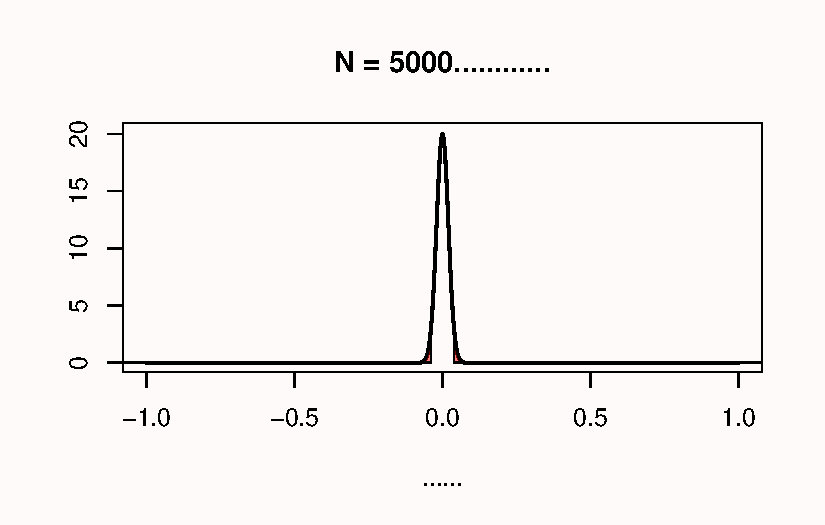
\includegraphics[width=1\textwidth,height=\textheight]{01-pvalue_files/figure-pdf/fig-fig132-1.pdf}

}

\caption{\label{fig-fig132}当d=0时,在每组收集5000个观察值的独立样本t检验中,所得Cohen's
\emph{d}效应量的分布。}

\end{figure}

由于均值差的分布是基于均值差的标准误,所以5000样本量的分布要窄得多。这个值是根据标准差和样本量计算的,如下所示:

\[\sqrt{\frac{\sigma_{1}^{2}}{n_{1}}+\frac{\sigma_{2}^{2}}{n_{2}}}\]
这个公式表明,均值差的标准误是每个组的标准差(σ)的平方除以该组的样本量,加在一起,然后取平方根。样本量越大,除以的数字就越大,因此均值差的标准误就越小。在n
=50的例子中,有标准差:

\[\sqrt{\frac{1^{2}}{50}+\frac{1^{2}}{50}}\] 因此,当n =
50时,两组均值差的标准误为0.2;当n =
5000时,均值差的标准误为0.02。假设抽样分布为正态分布,95\%的观测值落在1.96
个标准误之间。因此,对于样本量为50的样本,均值差应该在-1.96 * 0.2 =
-0.392和+1.96 * 0.2 = 0.392之间,我们可以看到,当n =
50时,红色区域大约从-0.392到0.392。对于样本量为5000的样本,均值差应在-1.96
* 0.02和+1.96 *
0.02之间,也就是说,应该介于-0.0392到0.0392之间。由于样本量较大(n =
5000),观测得到的均值差应该比较小样本(n=50)中观测得到的均值差更接近0.

如果我们抽出n =
5000的样本,并且观测到0.5的均值差,我们要清楚,这样的概率比起收集50个观测值发现0.5的均值差的要更小。我们现在几乎已经准备好介绍关于p值的常见误解,但在此之前,我们需要引入一个当零假设不为真时的数据模型。如果我们不是从一个真实均值差为0的模型中抽样,那么得到的备择模型会是什么样呢?一些软件
(比如 G*power, 见 图
@ref(fig:gpowerscreenshot))会同时显示出零模型(红色曲线)和备择模型(蓝色曲线):

(ref:gpowerscreenshotlab)
G*Power软件截图显示了零模型(红色分布)和备择模型(蓝色分布)以及区分显著和非显著结果的临界\emph{t}值(1.66055)。

(ref:gpowerscreenshotlab) Screenshot from G*Power software visualizing
the null model (red distribution) and alternative model (blue
distribution) and the critical \emph{t}-value (1.66055) that is the
threshold distinguishing significant and non-significant results.

\begin{figure}

{\centering \includegraphics[width=1\textwidth,height=\textheight]{images/1.3.3.png}

}

\caption{\label{fig-gpowerscreenshot}G*Power软件截图显示了零模型(红色分布)和备择模型(蓝色分布)以及区分显著和非显著结果的临界\emph{t}值(1.66055)。}

\end{figure}

当我们做一项研究时,我们不知道真正的均值差是多少(如果我们已经知道了,为什么还要做这项研究?)但是,让我们假设有一个全知的存在,按照Paul
Meehl的说法,我们称呼祂为''无所不知的琼斯''。在我们从总体里收集50个观测值之前,``无所不知的琼斯''就已经知道了总体的真实均值差为0.5。那么在备择模型中,均差值就应该在0.5周围变化。下图显示了零假设成立时的数据模式(用灰线表示),和备择模型(用黑线表示),即假设总体中存在0.5的真实均值差的模型。

\begin{verbatim}
Warning in title(...): conversion failure on 'N = 50 的零假设和备择假设' in
'mbcsToSbcs': dot substituted for <e7>
\end{verbatim}

\begin{verbatim}
Warning in title(...): conversion failure on 'N = 50 的零假设和备择假设' in
'mbcsToSbcs': dot substituted for <9a>
\end{verbatim}

\begin{verbatim}
Warning in title(...): conversion failure on 'N = 50 的零假设和备择假设' in
'mbcsToSbcs': dot substituted for <84>
\end{verbatim}

\begin{verbatim}
Warning in title(...): conversion failure on 'N = 50 的零假设和备择假设' in
'mbcsToSbcs': dot substituted for <e9>
\end{verbatim}

\begin{verbatim}
Warning in title(...): conversion failure on 'N = 50 的零假设和备择假设' in
'mbcsToSbcs': dot substituted for <9b>
\end{verbatim}

\begin{verbatim}
Warning in title(...): conversion failure on 'N = 50 的零假设和备择假设' in
'mbcsToSbcs': dot substituted for <b6>
\end{verbatim}

\begin{verbatim}
Warning in title(...): conversion failure on 'N = 50 的零假设和备择假设' in
'mbcsToSbcs': dot substituted for <e5>
\end{verbatim}

\begin{verbatim}
Warning in title(...): conversion failure on 'N = 50 的零假设和备择假设' in
'mbcsToSbcs': dot substituted for <81>
\end{verbatim}

\begin{verbatim}
Warning in title(...): conversion failure on 'N = 50 的零假设和备择假设' in
'mbcsToSbcs': dot substituted for <87>
\end{verbatim}

\begin{verbatim}
Warning in title(...): conversion failure on 'N = 50 的零假设和备择假设' in
'mbcsToSbcs': dot substituted for <e8>
\end{verbatim}

\begin{verbatim}
Warning in title(...): conversion failure on 'N = 50 的零假设和备择假设' in
'mbcsToSbcs': dot substituted for <ae>
\end{verbatim}

\begin{verbatim}
Warning in title(...): conversion failure on 'N = 50 的零假设和备择假设' in
'mbcsToSbcs': dot substituted for <be>
\end{verbatim}

\begin{verbatim}
Warning in title(...): conversion failure on 'N = 50 的零假设和备择假设' in
'mbcsToSbcs': dot substituted for <e5>
\end{verbatim}

\begin{verbatim}
Warning in title(...): conversion failure on 'N = 50 的零假设和备择假设' in
'mbcsToSbcs': dot substituted for <92>
\end{verbatim}

\begin{verbatim}
Warning in title(...): conversion failure on 'N = 50 的零假设和备择假设' in
'mbcsToSbcs': dot substituted for <8c>
\end{verbatim}

\begin{verbatim}
Warning in title(...): conversion failure on 'N = 50 的零假设和备择假设' in
'mbcsToSbcs': dot substituted for <e5>
\end{verbatim}

\begin{verbatim}
Warning in title(...): conversion failure on 'N = 50 的零假设和备择假设' in
'mbcsToSbcs': dot substituted for <a4>
\end{verbatim}

\begin{verbatim}
Warning in title(...): conversion failure on 'N = 50 的零假设和备择假设' in
'mbcsToSbcs': dot substituted for <87>
\end{verbatim}

\begin{verbatim}
Warning in title(...): conversion failure on 'N = 50 的零假设和备择假设' in
'mbcsToSbcs': dot substituted for <e6>
\end{verbatim}

\begin{verbatim}
Warning in title(...): conversion failure on 'N = 50 的零假设和备择假设' in
'mbcsToSbcs': dot substituted for <8b>
\end{verbatim}

\begin{verbatim}
Warning in title(...): conversion failure on 'N = 50 的零假设和备择假设' in
'mbcsToSbcs': dot substituted for <a9>
\end{verbatim}

\begin{verbatim}
Warning in title(...): conversion failure on 'N = 50 的零假设和备择假设' in
'mbcsToSbcs': dot substituted for <e5>
\end{verbatim}

\begin{verbatim}
Warning in title(...): conversion failure on 'N = 50 的零假设和备择假设' in
'mbcsToSbcs': dot substituted for <81>
\end{verbatim}

\begin{verbatim}
Warning in title(...): conversion failure on 'N = 50 的零假设和备择假设' in
'mbcsToSbcs': dot substituted for <87>
\end{verbatim}

\begin{verbatim}
Warning in title(...): conversion failure on 'N = 50 的零假设和备择假设' in
'mbcsToSbcs': dot substituted for <e8>
\end{verbatim}

\begin{verbatim}
Warning in title(...): conversion failure on 'N = 50 的零假设和备择假设' in
'mbcsToSbcs': dot substituted for <ae>
\end{verbatim}

\begin{verbatim}
Warning in title(...): conversion failure on 'N = 50 的零假设和备择假设' in
'mbcsToSbcs': dot substituted for <be>
\end{verbatim}

\begin{verbatim}
Warning in title(...): conversion failure on '差异' in 'mbcsToSbcs': dot
substituted for <e5>
\end{verbatim}

\begin{verbatim}
Warning in title(...): conversion failure on '差异' in 'mbcsToSbcs': dot
substituted for <b7>
\end{verbatim}

\begin{verbatim}
Warning in title(...): conversion failure on '差异' in 'mbcsToSbcs': dot
substituted for <ae>
\end{verbatim}

\begin{verbatim}
Warning in title(...): conversion failure on '差异' in 'mbcsToSbcs': dot
substituted for <e5>
\end{verbatim}

\begin{verbatim}
Warning in title(...): conversion failure on '差异' in 'mbcsToSbcs': dot
substituted for <bc>
\end{verbatim}

\begin{verbatim}
Warning in title(...): conversion failure on '差异' in 'mbcsToSbcs': dot
substituted for <82>
\end{verbatim}

\begin{figure}

{\centering \includegraphics[width=1\textwidth,height=\textheight]{01-pvalue_files/figure-pdf/fig-fig134-1.pdf}

}

\caption{\label{fig-fig134}在\emph{d} =
0,每组收集50个观测值的独立样本\emph{t}检验中,Cohen's
\emph{d}效应量的分布。}

\end{figure}

但是''无所不知的琼斯''也可以说真实均值差是一个更大的值。假设在另一个研究中,在我们抽样之前,祂就说真实均值差是1.5。那么此时零假设模型不变,备择假设模型会向右移动。

您可以在此应用程序上在线调整备择模型和零模型:\url{http://shiny.ieis.tue.nl/d_p_power/}.
该应用程序允许你设定参加t检验的两组的样本量(从2到无穷大)、均值差(从0到2)和alpha水平。在图中,红色区域表示I类错误,蓝色区域表示II类错误(具体我们将在之后讨论)。该应用程序也会显示临界值:会有一条垂直线(样本量为50时,落在均值差为0.4处)和一句提示语------大于0.4代表效应显著。虽然没有提示语,我们应该知道此时小于-0.4也显著。这个应用程序也适用于双侧的独立t检验。

你可以看到,在表示临界均值差的竖线的左边有一个蓝色区域,它是备择模型的一部分。这就是犯II类错误的概率(或者代表1-统计力)。如果一个研究的统计力是80\%,代表我们能观测到的80\%的均值差都会落在代表临界值的那条线的右边。如果备择假设为真,但是我们又得到了小于临界值的效应,那么即使真的存在效应,此时的\emph{p}值应该大于0.05。你可以在应用程序中验证,当样本量越大,整个备择模型就越靠右,统计力也就越大。同时你也可以看到,样本量越大,分布越窄,低于临界值的分布越少(只要真实总体均值大于临界值)。最终,α水平越大,临界值代表的均值差越向左移,低于临界值的备择分布的面积就越小。

该应用程序还绘制了3个图,是不同α水平、不同样本量和不同真均值差下的功率曲线函数。用户可以在应用程序中调整这三个值,了解每个变量如何影响零模型和备择模型,看到达到统计水平上显著的均值差的大小和犯Ⅰ类以和Ⅱ类错误的概率。

到目前为止,零模型的几个方面应该已经变得逐渐清晰。首先,传统零假设中,总体均值差为0,但在你抽出的任何样本中,观测的均值差都落在一个以0为中心的分布中,通常会略大于或略小于0。其次,该分布的宽度取决于样本量和标准差。研究的样本量越大,分布就越集中于0。最后,当观测到的均值差落在零模型尾端时,结果被认为是出人意料的。离0越远,这个结果就越令人惊讶。但是,当零模型为真时,这些令人惊讶的结果发生的概率为α水平(也被称为Ⅰ类错误)。请记住,当研究人员得出总体存在差异时,但实际的均值差为0时,就会发生第一类错误。

我们现在终于准备好可以厘清一些关于\emph{p}值的常见误解了。让我们来回顾一下科学文献中报告过的一系列常见误解。其中一些也许听起来只是语言表达问题。乍一看,人们很容易认为这句话传达了正确的想法,即使在书面形式上并不正确。然而,当一个陈述在形式上不正确时,它就是错误的。正是因为人们会经常误解\emph{p}值,所以在形式上正确解释\emph{p}值是非常重要的。

\hypertarget{sec-misconception1}{%
\subsection{\texorpdfstring{误解
1:\emph{p}值不显著意味着零假设为真。}{误解 1:p值不显著意味着零假设为真。}}\label{sec-misconception1}}

此误解的一个常见版本体现在句子'因为\emph{p} \textgreater{} 0.05,
我们可以推断效应不存在'中;这句话也可以是'差异不存在(\emph{p}
\textgreater{} 0.05)'。

在谈论细节之前,我想提醒你一个简单的事实,它会使你辨明许多关于\emph{p}值的误解:p值是有关数据概率的解释,而非一个假设或理论的概率的解释。不论何时你看到\emph{p}值被用于解释一个假设或理论的概率,你就知道事情有些不太对。有关假设的例子有:`零假设为真'或'备择假设为真',它们都是指零模型或者备择模型为真的概率是100\%。更微妙的表述有'观测到的差异不是出于偶然'。当零假设为真时,观测到的差异只是'由于偶然'(而不是由于真实差异的存在),与之前一样,这句话是指零假设100\%为真。

当你得出'效应不存在'或者'不存在差异'的结论时,你也就是在说零假设100\%为真。但是由于\emph{p}值是有关数据概率的解释,你应该避免仅基于\emph{p}值去解释理论存在的概率。\emph{p}值的设计是用来帮助你识别嘈杂的数据生成(即真实情况)中意料之外的结果。它并不能量化一个假设为真的概率。

让我们举一个具体的例子来说明为什么不显著的结果并不意味着零假设就是正确的。在下图中,无所不知的琼斯告诉我们,真均值差为0.5。我们可以从图中看出,当备择假设为真时,期望的均值差的可视化分布以0.5为中心。我们观测到的均值差是0.35。这个值还没有极端到足以在统计学上与0有显著差异。同样从图中可以看出,这个值没有落在零模型的红色区域(因此,\emph{p}值并不小于我们规定的α水平)。

然而,鉴于真均值差是0.5,观测均值差为0.35不光很可能发生,更可能是在备择模型而非是零模型上观测到。你可以看到这一点,因为在零模型中,均值差为0.35的概率密度曲线的高度约为0.5,在备择模型中概率密度曲线的高度则接近1.5。详情请参见\protect\hyperlink{likettest}{可能性}一章。

\begin{verbatim}
Warning in title(...): conversion failure on 'N = 50 的零假设和备择假设' in
'mbcsToSbcs': dot substituted for <e7>
\end{verbatim}

\begin{verbatim}
Warning in title(...): conversion failure on 'N = 50 的零假设和备择假设' in
'mbcsToSbcs': dot substituted for <9a>
\end{verbatim}

\begin{verbatim}
Warning in title(...): conversion failure on 'N = 50 的零假设和备择假设' in
'mbcsToSbcs': dot substituted for <84>
\end{verbatim}

\begin{verbatim}
Warning in title(...): conversion failure on 'N = 50 的零假设和备择假设' in
'mbcsToSbcs': dot substituted for <e9>
\end{verbatim}

\begin{verbatim}
Warning in title(...): conversion failure on 'N = 50 的零假设和备择假设' in
'mbcsToSbcs': dot substituted for <9b>
\end{verbatim}

\begin{verbatim}
Warning in title(...): conversion failure on 'N = 50 的零假设和备择假设' in
'mbcsToSbcs': dot substituted for <b6>
\end{verbatim}

\begin{verbatim}
Warning in title(...): conversion failure on 'N = 50 的零假设和备择假设' in
'mbcsToSbcs': dot substituted for <e5>
\end{verbatim}

\begin{verbatim}
Warning in title(...): conversion failure on 'N = 50 的零假设和备择假设' in
'mbcsToSbcs': dot substituted for <81>
\end{verbatim}

\begin{verbatim}
Warning in title(...): conversion failure on 'N = 50 的零假设和备择假设' in
'mbcsToSbcs': dot substituted for <87>
\end{verbatim}

\begin{verbatim}
Warning in title(...): conversion failure on 'N = 50 的零假设和备择假设' in
'mbcsToSbcs': dot substituted for <e8>
\end{verbatim}

\begin{verbatim}
Warning in title(...): conversion failure on 'N = 50 的零假设和备择假设' in
'mbcsToSbcs': dot substituted for <ae>
\end{verbatim}

\begin{verbatim}
Warning in title(...): conversion failure on 'N = 50 的零假设和备择假设' in
'mbcsToSbcs': dot substituted for <be>
\end{verbatim}

\begin{verbatim}
Warning in title(...): conversion failure on 'N = 50 的零假设和备择假设' in
'mbcsToSbcs': dot substituted for <e5>
\end{verbatim}

\begin{verbatim}
Warning in title(...): conversion failure on 'N = 50 的零假设和备择假设' in
'mbcsToSbcs': dot substituted for <92>
\end{verbatim}

\begin{verbatim}
Warning in title(...): conversion failure on 'N = 50 的零假设和备择假设' in
'mbcsToSbcs': dot substituted for <8c>
\end{verbatim}

\begin{verbatim}
Warning in title(...): conversion failure on 'N = 50 的零假设和备择假设' in
'mbcsToSbcs': dot substituted for <e5>
\end{verbatim}

\begin{verbatim}
Warning in title(...): conversion failure on 'N = 50 的零假设和备择假设' in
'mbcsToSbcs': dot substituted for <a4>
\end{verbatim}

\begin{verbatim}
Warning in title(...): conversion failure on 'N = 50 的零假设和备择假设' in
'mbcsToSbcs': dot substituted for <87>
\end{verbatim}

\begin{verbatim}
Warning in title(...): conversion failure on 'N = 50 的零假设和备择假设' in
'mbcsToSbcs': dot substituted for <e6>
\end{verbatim}

\begin{verbatim}
Warning in title(...): conversion failure on 'N = 50 的零假设和备择假设' in
'mbcsToSbcs': dot substituted for <8b>
\end{verbatim}

\begin{verbatim}
Warning in title(...): conversion failure on 'N = 50 的零假设和备择假设' in
'mbcsToSbcs': dot substituted for <a9>
\end{verbatim}

\begin{verbatim}
Warning in title(...): conversion failure on 'N = 50 的零假设和备择假设' in
'mbcsToSbcs': dot substituted for <e5>
\end{verbatim}

\begin{verbatim}
Warning in title(...): conversion failure on 'N = 50 的零假设和备择假设' in
'mbcsToSbcs': dot substituted for <81>
\end{verbatim}

\begin{verbatim}
Warning in title(...): conversion failure on 'N = 50 的零假设和备择假设' in
'mbcsToSbcs': dot substituted for <87>
\end{verbatim}

\begin{verbatim}
Warning in title(...): conversion failure on 'N = 50 的零假设和备择假设' in
'mbcsToSbcs': dot substituted for <e8>
\end{verbatim}

\begin{verbatim}
Warning in title(...): conversion failure on 'N = 50 的零假设和备择假设' in
'mbcsToSbcs': dot substituted for <ae>
\end{verbatim}

\begin{verbatim}
Warning in title(...): conversion failure on 'N = 50 的零假设和备择假设' in
'mbcsToSbcs': dot substituted for <be>
\end{verbatim}

\begin{verbatim}
Warning in title(...): conversion failure on '差异' in 'mbcsToSbcs': dot
substituted for <e5>
\end{verbatim}

\begin{verbatim}
Warning in title(...): conversion failure on '差异' in 'mbcsToSbcs': dot
substituted for <b7>
\end{verbatim}

\begin{verbatim}
Warning in title(...): conversion failure on '差异' in 'mbcsToSbcs': dot
substituted for <ae>
\end{verbatim}

\begin{verbatim}
Warning in title(...): conversion failure on '差异' in 'mbcsToSbcs': dot
substituted for <e5>
\end{verbatim}

\begin{verbatim}
Warning in title(...): conversion failure on '差异' in 'mbcsToSbcs': dot
substituted for <bc>
\end{verbatim}

\begin{verbatim}
Warning in title(...): conversion failure on '差异' in 'mbcsToSbcs': dot
substituted for <82>
\end{verbatim}

\begin{verbatim}
Warning in text.default(0.35, 2.4, paste("所得均值差异"), cex = 1): conversion
failure on '所得均值差异' in 'mbcsToSbcs': dot substituted for <e6>
\end{verbatim}

\begin{verbatim}
Warning in text.default(0.35, 2.4, paste("所得均值差异"), cex = 1): conversion
failure on '所得均值差异' in 'mbcsToSbcs': dot substituted for <89>
\end{verbatim}

\begin{verbatim}
Warning in text.default(0.35, 2.4, paste("所得均值差异"), cex = 1): conversion
failure on '所得均值差异' in 'mbcsToSbcs': dot substituted for <80>
\end{verbatim}

\begin{verbatim}
Warning in text.default(0.35, 2.4, paste("所得均值差异"), cex = 1): conversion
failure on '所得均值差异' in 'mbcsToSbcs': dot substituted for <e5>
\end{verbatim}

\begin{verbatim}
Warning in text.default(0.35, 2.4, paste("所得均值差异"), cex = 1): conversion
failure on '所得均值差异' in 'mbcsToSbcs': dot substituted for <be>
\end{verbatim}

\begin{verbatim}
Warning in text.default(0.35, 2.4, paste("所得均值差异"), cex = 1): conversion
failure on '所得均值差异' in 'mbcsToSbcs': dot substituted for <97>
\end{verbatim}

\begin{verbatim}
Warning in text.default(0.35, 2.4, paste("所得均值差异"), cex = 1): conversion
failure on '所得均值差异' in 'mbcsToSbcs': dot substituted for <e5>
\end{verbatim}

\begin{verbatim}
Warning in text.default(0.35, 2.4, paste("所得均值差异"), cex = 1): conversion
failure on '所得均值差异' in 'mbcsToSbcs': dot substituted for <9d>
\end{verbatim}

\begin{verbatim}
Warning in text.default(0.35, 2.4, paste("所得均值差异"), cex = 1): conversion
failure on '所得均值差异' in 'mbcsToSbcs': dot substituted for <87>
\end{verbatim}

\begin{verbatim}
Warning in text.default(0.35, 2.4, paste("所得均值差异"), cex = 1): conversion
failure on '所得均值差异' in 'mbcsToSbcs': dot substituted for <e5>
\end{verbatim}

\begin{verbatim}
Warning in text.default(0.35, 2.4, paste("所得均值差异"), cex = 1): conversion
failure on '所得均值差异' in 'mbcsToSbcs': dot substituted for <80>
\end{verbatim}

\begin{verbatim}
Warning in text.default(0.35, 2.4, paste("所得均值差异"), cex = 1): conversion
failure on '所得均值差异' in 'mbcsToSbcs': dot substituted for <bc>
\end{verbatim}

\begin{verbatim}
Warning in text.default(0.35, 2.4, paste("所得均值差异"), cex = 1): conversion
failure on '所得均值差异' in 'mbcsToSbcs': dot substituted for <e5>
\end{verbatim}

\begin{verbatim}
Warning in text.default(0.35, 2.4, paste("所得均值差异"), cex = 1): conversion
failure on '所得均值差异' in 'mbcsToSbcs': dot substituted for <b7>
\end{verbatim}

\begin{verbatim}
Warning in text.default(0.35, 2.4, paste("所得均值差异"), cex = 1): conversion
failure on '所得均值差异' in 'mbcsToSbcs': dot substituted for <ae>
\end{verbatim}

\begin{verbatim}
Warning in text.default(0.35, 2.4, paste("所得均值差异"), cex = 1): conversion
failure on '所得均值差异' in 'mbcsToSbcs': dot substituted for <e5>
\end{verbatim}

\begin{verbatim}
Warning in text.default(0.35, 2.4, paste("所得均值差异"), cex = 1): conversion
failure on '所得均值差异' in 'mbcsToSbcs': dot substituted for <bc>
\end{verbatim}

\begin{verbatim}
Warning in text.default(0.35, 2.4, paste("所得均值差异"), cex = 1): conversion
failure on '所得均值差异' in 'mbcsToSbcs': dot substituted for <82>
\end{verbatim}

\begin{verbatim}
Warning in text.default(0.35, 2.4, paste("所得均值差异"), cex = 1): font
metrics unknown for Unicode character U+6240
\end{verbatim}

\begin{verbatim}
Warning in text.default(0.35, 2.4, paste("所得均值差异"), cex = 1): font
metrics unknown for Unicode character U+5f97
\end{verbatim}

\begin{verbatim}
Warning in text.default(0.35, 2.4, paste("所得均值差异"), cex = 1): font
metrics unknown for Unicode character U+5747
\end{verbatim}

\begin{verbatim}
Warning in text.default(0.35, 2.4, paste("所得均值差异"), cex = 1): font
metrics unknown for Unicode character U+503c
\end{verbatim}

\begin{verbatim}
Warning in text.default(0.35, 2.4, paste("所得均值差异"), cex = 1): font
metrics unknown for Unicode character U+5dee
\end{verbatim}

\begin{verbatim}
Warning in text.default(0.35, 2.4, paste("所得均值差异"), cex = 1): font
metrics unknown for Unicode character U+5f02
\end{verbatim}

\begin{figure}

{\centering \includegraphics[width=1\textwidth,height=\textheight]{01-pvalue_files/figure-pdf/fig-fig136-1.pdf}

}

\caption{\label{fig-fig136}在\emph{d} = 0.35时,对\emph{d} = 0和\emph{d}
= 0.5进行每组50个观测值的独立样本t检验,所得Cohen's
\emph{d}效应量的分布。}

\end{figure}

如果我们假定零假设为真,所有的p值都告诉我们均值差为0.35并不是非常出人意料。这可能有很多原因。在真实世界中,并不存在无所不知的琼斯告诉我们真均值差,就像上图所示,有可能存在一个真实效应。

那么我们应该怎么陈述呢?解决方案很微妙,但也很重要。让我们再看看之前做的两个错误陈述的例子。首先,``因为\emph{p}
\textgreater{}
0.05,我们可以推断效应不存在''这个陈述是错误的,因为很有可能效应是存在的(请记住\emph{p}值是有关数据的解释而不是有效应或无效应的概率)。
费希尔对于p值的解释是我们可以得出一个小概率事件的发生或者零假设是错误的(他的原话是:``要么是发生了及其罕见的事件,要么是随机分布的原假设不正确'')。这可能听起来像是有关理论的概率的解释,但实际只是在p值很小时,对两种可能出现的场景的陈述(你犯Ⅰ型错误或者备择假设才为真)。真阳性和假阳性都是可能的,并且我们不量化两种可能性出现的概率(例如,并不是说零假设为真的概率是95\%)。从内曼-皮尔逊的角度,p
\textgreater{}
.05意味着我们不能拒绝零假设,因为我们有着5\%以下的预期错误率。

如果你对于推断效应缺失感兴趣,零假设检验不是你需要的工具。零假设检验回答的问题是'在期望的错误率下,我可以拒绝零假设吗?'。当\emph{p}
\textgreater{}
0.05,你不能拒绝零假设时,零假设是真还是假是不能仅仅基于\emph{p}值得出的(就像'无'的概念:既不是真也不是假)。幸运地是,已经开发了别的统计方法来回答效应缺失的问题,例如
\protect\hyperlink{equivalencetest}{等效检验}, 贝叶斯因子和贝叶斯估计
(请参见 Harms \& Lakens (2018), 了解概述).

第二个不正确的说法是'没有差异'。这个陈述改正起来要容易些。你可以写'没有统计学上的显著差异'。当然,两者有点重复,因为你基本上在用两种不同的方式说\emph{p}值大于α水平,但至少这个说法在形式上是正确的。`没有差异'和'没有统计学上的显著差异'可能听起来差不多,但前者你实际上在说'差异为0',而后者你是在说'差异不足以使\emph{p}
\textless{}
.05'。虽然我从未见过有人这样做,但是更完整的说法应该是'鉴于样本量是每组50,α水平是0.05,观测差异只有大于0.4才能达到统计学上的显著,由于我们观测的差异是0.35,因此我们不能拒绝零假设'。如果这看起来不是一个令人满意的结论,请记住,零假设检验的设计不是为了得出效应缺失的有趣结论------你需要了解等效检验,来得到有关零效应更令人满意的答案。

\hypertarget{ux8befux89e3-2pux503cux663eux8457ux610fux5473ux7740ux96f6ux5047ux8bbeux4e3aux5047}{%
\subsection{\texorpdfstring{误解
2:\emph{p}值显著意味着零假设为假。}{误解 2:p值显著意味着零假设为假。}}\label{ux8befux89e3-2pux503cux663eux8457ux610fux5473ux7740ux96f6ux5047ux8bbeux4e3aux5047}}

这是上一个误解的另一面。基于这种误解的错误陈述有'\emph{p} \textless{}
.05,因此效应存在',或'两组之间存在差异,\emph{p} \textless{}
.05'。像之前一样,这些陈述都是在暗指零假设为假的概率是100\%,备择假设才为真。

举一个简单的例子,说明为什么这些极端的语句是不正确的。假设我们使用下面的命令在R中生成一系列数字:

\begin{Shaded}
\begin{Highlighting}[]
\FunctionTok{rnorm}\NormalTok{(}\AttributeTok{n =} \DecValTok{50}\NormalTok{, }\AttributeTok{mean =} \DecValTok{0}\NormalTok{, }\AttributeTok{sd =} \DecValTok{1}\NormalTok{)}
\end{Highlighting}
\end{Shaded}

\begin{verbatim}
 [1]  0.4719836  1.1920227  1.7721923  2.1265877 -0.4252310 -0.6015820
 [7] -0.7724946  2.1346629 -1.0146817 -1.9681660  0.4141101 -0.7775625
[13] -0.8676887 -2.9356859 -0.7683710  0.2427153 -1.6955546 -1.0225851
[19]  0.8434979  0.9441817 -1.1777169  0.5389057  1.3519592  0.1506133
[25]  0.5847717  1.3628052  0.2540480 -0.3172475  0.6699546 -0.5790094
[31]  0.2308175 -0.5749606  1.1622497  0.9164392 -0.7536052  0.0411087
[37]  0.4761396  1.5822320 -0.7285862  0.2672048  1.1460240 -0.4623852
[43] -0.3431018  1.2740455 -0.2109466  0.4215509 -0.9884471  1.5876178
[49]  0.1934516  1.1746930
\end{verbatim}

该命令会从一个平均值为0、标准差为1的分布中随机生成50个观察值(从长远来看------生成的每个样本的平均值和标准差都会有所不同)。想象我们运行这个命令一次,得到一个平均值为0.5的分布。下面的图画出了这个分布。假设我们可以做它和0的单样本t检验,得到\emph{p}
\textless{}
.05,此检验告诉我们,我们观测到的数据与0有显著差异,但此时R函数中随机数生成器依然按照原来的指令运行,生成的数据的真实均值为0。

\begin{verbatim}
Warning in title(...): conversion failure on 'N = 50 的零假设和备择假设' in
'mbcsToSbcs': dot substituted for <e7>
\end{verbatim}

\begin{verbatim}
Warning in title(...): conversion failure on 'N = 50 的零假设和备择假设' in
'mbcsToSbcs': dot substituted for <9a>
\end{verbatim}

\begin{verbatim}
Warning in title(...): conversion failure on 'N = 50 的零假设和备择假设' in
'mbcsToSbcs': dot substituted for <84>
\end{verbatim}

\begin{verbatim}
Warning in title(...): conversion failure on 'N = 50 的零假设和备择假设' in
'mbcsToSbcs': dot substituted for <e9>
\end{verbatim}

\begin{verbatim}
Warning in title(...): conversion failure on 'N = 50 的零假设和备择假设' in
'mbcsToSbcs': dot substituted for <9b>
\end{verbatim}

\begin{verbatim}
Warning in title(...): conversion failure on 'N = 50 的零假设和备择假设' in
'mbcsToSbcs': dot substituted for <b6>
\end{verbatim}

\begin{verbatim}
Warning in title(...): conversion failure on 'N = 50 的零假设和备择假设' in
'mbcsToSbcs': dot substituted for <e5>
\end{verbatim}

\begin{verbatim}
Warning in title(...): conversion failure on 'N = 50 的零假设和备择假设' in
'mbcsToSbcs': dot substituted for <81>
\end{verbatim}

\begin{verbatim}
Warning in title(...): conversion failure on 'N = 50 的零假设和备择假设' in
'mbcsToSbcs': dot substituted for <87>
\end{verbatim}

\begin{verbatim}
Warning in title(...): conversion failure on 'N = 50 的零假设和备择假设' in
'mbcsToSbcs': dot substituted for <e8>
\end{verbatim}

\begin{verbatim}
Warning in title(...): conversion failure on 'N = 50 的零假设和备择假设' in
'mbcsToSbcs': dot substituted for <ae>
\end{verbatim}

\begin{verbatim}
Warning in title(...): conversion failure on 'N = 50 的零假设和备择假设' in
'mbcsToSbcs': dot substituted for <be>
\end{verbatim}

\begin{verbatim}
Warning in title(...): conversion failure on 'N = 50 的零假设和备择假设' in
'mbcsToSbcs': dot substituted for <e5>
\end{verbatim}

\begin{verbatim}
Warning in title(...): conversion failure on 'N = 50 的零假设和备择假设' in
'mbcsToSbcs': dot substituted for <92>
\end{verbatim}

\begin{verbatim}
Warning in title(...): conversion failure on 'N = 50 的零假设和备择假设' in
'mbcsToSbcs': dot substituted for <8c>
\end{verbatim}

\begin{verbatim}
Warning in title(...): conversion failure on 'N = 50 的零假设和备择假设' in
'mbcsToSbcs': dot substituted for <e5>
\end{verbatim}

\begin{verbatim}
Warning in title(...): conversion failure on 'N = 50 的零假设和备择假设' in
'mbcsToSbcs': dot substituted for <a4>
\end{verbatim}

\begin{verbatim}
Warning in title(...): conversion failure on 'N = 50 的零假设和备择假设' in
'mbcsToSbcs': dot substituted for <87>
\end{verbatim}

\begin{verbatim}
Warning in title(...): conversion failure on 'N = 50 的零假设和备择假设' in
'mbcsToSbcs': dot substituted for <e6>
\end{verbatim}

\begin{verbatim}
Warning in title(...): conversion failure on 'N = 50 的零假设和备择假设' in
'mbcsToSbcs': dot substituted for <8b>
\end{verbatim}

\begin{verbatim}
Warning in title(...): conversion failure on 'N = 50 的零假设和备择假设' in
'mbcsToSbcs': dot substituted for <a9>
\end{verbatim}

\begin{verbatim}
Warning in title(...): conversion failure on 'N = 50 的零假设和备择假设' in
'mbcsToSbcs': dot substituted for <e5>
\end{verbatim}

\begin{verbatim}
Warning in title(...): conversion failure on 'N = 50 的零假设和备择假设' in
'mbcsToSbcs': dot substituted for <81>
\end{verbatim}

\begin{verbatim}
Warning in title(...): conversion failure on 'N = 50 的零假设和备择假设' in
'mbcsToSbcs': dot substituted for <87>
\end{verbatim}

\begin{verbatim}
Warning in title(...): conversion failure on 'N = 50 的零假设和备择假设' in
'mbcsToSbcs': dot substituted for <e8>
\end{verbatim}

\begin{verbatim}
Warning in title(...): conversion failure on 'N = 50 的零假设和备择假设' in
'mbcsToSbcs': dot substituted for <ae>
\end{verbatim}

\begin{verbatim}
Warning in title(...): conversion failure on 'N = 50 的零假设和备择假设' in
'mbcsToSbcs': dot substituted for <be>
\end{verbatim}

\begin{verbatim}
Warning in title(...): conversion failure on '差异' in 'mbcsToSbcs': dot
substituted for <e5>
\end{verbatim}

\begin{verbatim}
Warning in title(...): conversion failure on '差异' in 'mbcsToSbcs': dot
substituted for <b7>
\end{verbatim}

\begin{verbatim}
Warning in title(...): conversion failure on '差异' in 'mbcsToSbcs': dot
substituted for <ae>
\end{verbatim}

\begin{verbatim}
Warning in title(...): conversion failure on '差异' in 'mbcsToSbcs': dot
substituted for <e5>
\end{verbatim}

\begin{verbatim}
Warning in title(...): conversion failure on '差异' in 'mbcsToSbcs': dot
substituted for <bc>
\end{verbatim}

\begin{verbatim}
Warning in title(...): conversion failure on '差异' in 'mbcsToSbcs': dot
substituted for <82>
\end{verbatim}

\begin{verbatim}
Warning in text.default(0.5, 2.4, paste("所得均值差异"), cex = 1): conversion
failure on '所得均值差异' in 'mbcsToSbcs': dot substituted for <e6>
\end{verbatim}

\begin{verbatim}
Warning in text.default(0.5, 2.4, paste("所得均值差异"), cex = 1): conversion
failure on '所得均值差异' in 'mbcsToSbcs': dot substituted for <89>
\end{verbatim}

\begin{verbatim}
Warning in text.default(0.5, 2.4, paste("所得均值差异"), cex = 1): conversion
failure on '所得均值差异' in 'mbcsToSbcs': dot substituted for <80>
\end{verbatim}

\begin{verbatim}
Warning in text.default(0.5, 2.4, paste("所得均值差异"), cex = 1): conversion
failure on '所得均值差异' in 'mbcsToSbcs': dot substituted for <e5>
\end{verbatim}

\begin{verbatim}
Warning in text.default(0.5, 2.4, paste("所得均值差异"), cex = 1): conversion
failure on '所得均值差异' in 'mbcsToSbcs': dot substituted for <be>
\end{verbatim}

\begin{verbatim}
Warning in text.default(0.5, 2.4, paste("所得均值差异"), cex = 1): conversion
failure on '所得均值差异' in 'mbcsToSbcs': dot substituted for <97>
\end{verbatim}

\begin{verbatim}
Warning in text.default(0.5, 2.4, paste("所得均值差异"), cex = 1): conversion
failure on '所得均值差异' in 'mbcsToSbcs': dot substituted for <e5>
\end{verbatim}

\begin{verbatim}
Warning in text.default(0.5, 2.4, paste("所得均值差异"), cex = 1): conversion
failure on '所得均值差异' in 'mbcsToSbcs': dot substituted for <9d>
\end{verbatim}

\begin{verbatim}
Warning in text.default(0.5, 2.4, paste("所得均值差异"), cex = 1): conversion
failure on '所得均值差异' in 'mbcsToSbcs': dot substituted for <87>
\end{verbatim}

\begin{verbatim}
Warning in text.default(0.5, 2.4, paste("所得均值差异"), cex = 1): conversion
failure on '所得均值差异' in 'mbcsToSbcs': dot substituted for <e5>
\end{verbatim}

\begin{verbatim}
Warning in text.default(0.5, 2.4, paste("所得均值差异"), cex = 1): conversion
failure on '所得均值差异' in 'mbcsToSbcs': dot substituted for <80>
\end{verbatim}

\begin{verbatim}
Warning in text.default(0.5, 2.4, paste("所得均值差异"), cex = 1): conversion
failure on '所得均值差异' in 'mbcsToSbcs': dot substituted for <bc>
\end{verbatim}

\begin{verbatim}
Warning in text.default(0.5, 2.4, paste("所得均值差异"), cex = 1): conversion
failure on '所得均值差异' in 'mbcsToSbcs': dot substituted for <e5>
\end{verbatim}

\begin{verbatim}
Warning in text.default(0.5, 2.4, paste("所得均值差异"), cex = 1): conversion
failure on '所得均值差异' in 'mbcsToSbcs': dot substituted for <b7>
\end{verbatim}

\begin{verbatim}
Warning in text.default(0.5, 2.4, paste("所得均值差异"), cex = 1): conversion
failure on '所得均值差异' in 'mbcsToSbcs': dot substituted for <ae>
\end{verbatim}

\begin{verbatim}
Warning in text.default(0.5, 2.4, paste("所得均值差异"), cex = 1): conversion
failure on '所得均值差异' in 'mbcsToSbcs': dot substituted for <e5>
\end{verbatim}

\begin{verbatim}
Warning in text.default(0.5, 2.4, paste("所得均值差异"), cex = 1): conversion
failure on '所得均值差异' in 'mbcsToSbcs': dot substituted for <bc>
\end{verbatim}

\begin{verbatim}
Warning in text.default(0.5, 2.4, paste("所得均值差异"), cex = 1): conversion
failure on '所得均值差异' in 'mbcsToSbcs': dot substituted for <82>
\end{verbatim}

\begin{verbatim}
Warning in text.default(0.5, 2.4, paste("所得均值差异"), cex = 1): font metrics
unknown for Unicode character U+6240
\end{verbatim}

\begin{verbatim}
Warning in text.default(0.5, 2.4, paste("所得均值差异"), cex = 1): font metrics
unknown for Unicode character U+5f97
\end{verbatim}

\begin{verbatim}
Warning in text.default(0.5, 2.4, paste("所得均值差异"), cex = 1): font metrics
unknown for Unicode character U+5747
\end{verbatim}

\begin{verbatim}
Warning in text.default(0.5, 2.4, paste("所得均值差异"), cex = 1): font metrics
unknown for Unicode character U+503c
\end{verbatim}

\begin{verbatim}
Warning in text.default(0.5, 2.4, paste("所得均值差异"), cex = 1): font metrics
unknown for Unicode character U+5dee
\end{verbatim}

\begin{verbatim}
Warning in text.default(0.5, 2.4, paste("所得均值差异"), cex = 1): font metrics
unknown for Unicode character U+5f02
\end{verbatim}

\begin{figure}

{\centering \includegraphics[width=1\textwidth,height=\textheight]{01-pvalue_files/figure-pdf/fig-fig137-1.pdf}

}

\caption{\label{fig-fig137}在\emph{d}= 0,对\emph{d} =
0.5进行每组50个观测值的独立样本\emph{t}检验中,所得Cohen's
\emph{d}效应量的分布}

\end{figure}

p值显著并不能让我们得出零假设(``随机数生成器照常运行'')为假的结论。的确,我们生成的50个样本的平均值是令人惊讶的极端值。但是较低的\emph{p}值只是告诉我们这个观测结果是出人意料的。当零假设为真时,我们只会在很低的概率下得到这个令人惊讶的观测结果------但它仍有可能发生。因此,显著的结果并不意味着备择假设就是对的------也有可能是出于Ⅰ型错误,就如同上面的例子,只有无所不知的琼斯知道是这种情况。

让我们重新审视这个错误陈述'\emph{p} \textless{}
.05,因此效应存在'。正确理解显著的\emph{p}值,要求我们承认显著结果是Ⅰ型错误的可能性。请记住,费希尔会得出的结论是''要么是发生了及其罕见的事件,要么是随机分布的原假设不正确''。对于内曼-皮尔逊统计的正确解释是:``我们可以当作零假设为假,从长远来看,我们错的时间不会超过5\%''。注意我们使用了'当作'这个词,这并不是在说任何特定的假设是真还是假,仅仅是指出,如果任何时候当\emph{p}
\textless{}
α,我们就当作零假设为假,那我们犯错误的频率将小于α百分比的时间。

这两种正式的陈述都有一点冗长。在科学文章中,我们经常读到简短点的陈述,比如:``我们可以拒绝零假设'',或者''我们可以接受备择假设''。这些陈述可能是假定读者会自己加上''长期来看,会有5\%的错误概率''这句话。但是,至少在第一次陈述时,可以加上''长期看有5\%的错误率''这个声明来提醒读者。

在上面的例子中,我们有一个非常强的主观先验概率,即R中的随机数生成器可以运行。其他可以纳入分析这种主观先验概率的统计方法有
\protect\hyperlink{bayes}{贝叶斯统计} 或者
\protect\hyperlink{ppv}{假阳报告概率}。在频率统计雪中,你需要多次重复你的研究。你会时不时地观测到Ⅰ类错误,但不太可能连续三次都观测到。或者,你也可以在单次研究中降低α水平,来降低犯Ⅰ类错误的概率。

\hypertarget{ux8befux89e3-3pux503cux663eux8457ux610fux5473ux7740ux53d1ux73b0ux4e86ux4e00ux4e2aux5b9eux9645ux91cdux8981ux7684ux6548ux5e94}{%
\subsection{\texorpdfstring{误解
3:\emph{p}值显著意味着发现了一个实际重要的效应。}{误解 3:p值显著意味着发现了一个实际重要的效应。}}\label{ux8befux89e3-3pux503cux663eux8457ux610fux5473ux7740ux53d1ux73b0ux4e86ux4e00ux4e2aux5b9eux9645ux91cdux8981ux7684ux6548ux5e94}}

在解释p值时,存在一个普遍的问题,即在日常语言中,``显著''意味着''重要'',因此''显著''的结果常被认为是一个''重要''的效应。然而,一个效应是否重要与它是否不等于零,或者说这个效应有多大是完全不同的两个问题。并不是所有的效应都用实际的影响。
这个效应越小,被人注意到的可能性就越小,但这个效应仍然可能会社会生产水平产生很大的影响。因此,正确的理解应该是,统计上的意义并不能回答一个效应在实践中是否重要,或者是否有''实际意义''的问题。要回答效应是否重要的问题,您需要进行成本效益分析。

这个实际意义的问题经常出现在样本量非常大的研究中。正如我们之前所看到的,随着样本量增加,零值周围的概率密度分布变得越来越窄,这被认为是\emph{p}值无限接近于0。

如果我们为一个非常大的样本量(例如,每组n=10000)绘制零模型,我们可以看到,即使是非常小的均值差(比0.04更极端的差异)也会被认为是''出人意料的''。这仍然意味着,如果在总体中真的没有差异,你观察到均值差大于0.04的将不到5\%的时间,在长期观测中,95\%的观测均值差将小于0.04。但是,要论证这种效应的实际意义就变得更加困难了。想象一下,一种特定的干预措施成功地改变了人们的消费行为,当实施这个干预措施时,人们每年可以节省12美分。很难说这种效应如何让任何一个个体感到开心。然而,如果把这笔资金加起来,它将产生超过200万美元,可用于治疗发展中国家的疾病,会产生很大的影响。如果我们的目标是让个人更快乐,干预的成本可能会被认为过高,但如果目标是为慈善机构筹集200万美元,它可能会被认为是值得的。

心理学中并不是所有的影响都是可以相加的(我们并不呢转移或者结合0.04的幸福感),因此往往很难论证主观感受中小效应的重要性(Anvari
et al.,
2021).。成本效益分析可能能显示很小的效应也很重要,但情况是否如此是不能从\emph{p}值中推断出来的。

请注意,这与对p值本身的解释并没有关系:如果零假设为真,p \textless{}
0.05仍然正确表明我们观测到的数据是出人意料的。然而,数据出人意料并不意味着我们就需要关心它。在这里造成困惑的主要是语言标签''显著''------``显著''应该理解为是''出乎意料的''效应,但不一定是''重要的''效应,这样想可能会减少困惑。

\hypertarget{sec-misconception4}{%
\subsection{误解
4:如果你得到了显著结果,你犯Ⅰ型错误(假阳性)的概率是5\%。}\label{sec-misconception4}}

此误解是对\emph{p}值是''偶然观察到显著结果的概率''这一错误说法的一种可能解释。试设想,我们收集了20个观测值,并且无所不知的琼斯告诉我们零假设为真(就像上面的例子里,我们在R中生成随机数一样)。这意味着我们正从下图的分布中进行抽样。

\begin{verbatim}
Warning in title(...): conversion failure on 'N = 20的零假设和备择假设' in
'mbcsToSbcs': dot substituted for <e7>
\end{verbatim}

\begin{verbatim}
Warning in title(...): conversion failure on 'N = 20的零假设和备择假设' in
'mbcsToSbcs': dot substituted for <9a>
\end{verbatim}

\begin{verbatim}
Warning in title(...): conversion failure on 'N = 20的零假设和备择假设' in
'mbcsToSbcs': dot substituted for <84>
\end{verbatim}

\begin{verbatim}
Warning in title(...): conversion failure on 'N = 20的零假设和备择假设' in
'mbcsToSbcs': dot substituted for <e9>
\end{verbatim}

\begin{verbatim}
Warning in title(...): conversion failure on 'N = 20的零假设和备择假设' in
'mbcsToSbcs': dot substituted for <9b>
\end{verbatim}

\begin{verbatim}
Warning in title(...): conversion failure on 'N = 20的零假设和备择假设' in
'mbcsToSbcs': dot substituted for <b6>
\end{verbatim}

\begin{verbatim}
Warning in title(...): conversion failure on 'N = 20的零假设和备择假设' in
'mbcsToSbcs': dot substituted for <e5>
\end{verbatim}

\begin{verbatim}
Warning in title(...): conversion failure on 'N = 20的零假设和备择假设' in
'mbcsToSbcs': dot substituted for <81>
\end{verbatim}

\begin{verbatim}
Warning in title(...): conversion failure on 'N = 20的零假设和备择假设' in
'mbcsToSbcs': dot substituted for <87>
\end{verbatim}

\begin{verbatim}
Warning in title(...): conversion failure on 'N = 20的零假设和备择假设' in
'mbcsToSbcs': dot substituted for <e8>
\end{verbatim}

\begin{verbatim}
Warning in title(...): conversion failure on 'N = 20的零假设和备择假设' in
'mbcsToSbcs': dot substituted for <ae>
\end{verbatim}

\begin{verbatim}
Warning in title(...): conversion failure on 'N = 20的零假设和备择假设' in
'mbcsToSbcs': dot substituted for <be>
\end{verbatim}

\begin{verbatim}
Warning in title(...): conversion failure on 'N = 20的零假设和备择假设' in
'mbcsToSbcs': dot substituted for <e5>
\end{verbatim}

\begin{verbatim}
Warning in title(...): conversion failure on 'N = 20的零假设和备择假设' in
'mbcsToSbcs': dot substituted for <92>
\end{verbatim}

\begin{verbatim}
Warning in title(...): conversion failure on 'N = 20的零假设和备择假设' in
'mbcsToSbcs': dot substituted for <8c>
\end{verbatim}

\begin{verbatim}
Warning in title(...): conversion failure on 'N = 20的零假设和备择假设' in
'mbcsToSbcs': dot substituted for <e5>
\end{verbatim}

\begin{verbatim}
Warning in title(...): conversion failure on 'N = 20的零假设和备择假设' in
'mbcsToSbcs': dot substituted for <a4>
\end{verbatim}

\begin{verbatim}
Warning in title(...): conversion failure on 'N = 20的零假设和备择假设' in
'mbcsToSbcs': dot substituted for <87>
\end{verbatim}

\begin{verbatim}
Warning in title(...): conversion failure on 'N = 20的零假设和备择假设' in
'mbcsToSbcs': dot substituted for <e6>
\end{verbatim}

\begin{verbatim}
Warning in title(...): conversion failure on 'N = 20的零假设和备择假设' in
'mbcsToSbcs': dot substituted for <8b>
\end{verbatim}

\begin{verbatim}
Warning in title(...): conversion failure on 'N = 20的零假设和备择假设' in
'mbcsToSbcs': dot substituted for <a9>
\end{verbatim}

\begin{verbatim}
Warning in title(...): conversion failure on 'N = 20的零假设和备择假设' in
'mbcsToSbcs': dot substituted for <e5>
\end{verbatim}

\begin{verbatim}
Warning in title(...): conversion failure on 'N = 20的零假设和备择假设' in
'mbcsToSbcs': dot substituted for <81>
\end{verbatim}

\begin{verbatim}
Warning in title(...): conversion failure on 'N = 20的零假设和备择假设' in
'mbcsToSbcs': dot substituted for <87>
\end{verbatim}

\begin{verbatim}
Warning in title(...): conversion failure on 'N = 20的零假设和备择假设' in
'mbcsToSbcs': dot substituted for <e8>
\end{verbatim}

\begin{verbatim}
Warning in title(...): conversion failure on 'N = 20的零假设和备择假设' in
'mbcsToSbcs': dot substituted for <ae>
\end{verbatim}

\begin{verbatim}
Warning in title(...): conversion failure on 'N = 20的零假设和备择假设' in
'mbcsToSbcs': dot substituted for <be>
\end{verbatim}

\begin{verbatim}
Warning in title(...): conversion failure on '差异' in 'mbcsToSbcs': dot
substituted for <e5>
\end{verbatim}

\begin{verbatim}
Warning in title(...): conversion failure on '差异' in 'mbcsToSbcs': dot
substituted for <b7>
\end{verbatim}

\begin{verbatim}
Warning in title(...): conversion failure on '差异' in 'mbcsToSbcs': dot
substituted for <ae>
\end{verbatim}

\begin{verbatim}
Warning in title(...): conversion failure on '差异' in 'mbcsToSbcs': dot
substituted for <e5>
\end{verbatim}

\begin{verbatim}
Warning in title(...): conversion failure on '差异' in 'mbcsToSbcs': dot
substituted for <bc>
\end{verbatim}

\begin{verbatim}
Warning in title(...): conversion failure on '差异' in 'mbcsToSbcs': dot
substituted for <82>
\end{verbatim}

\begin{verbatim}
Warning in text.default(0.5, 2.4, paste("所得均值差异"), cex = 1): conversion
failure on '所得均值差异' in 'mbcsToSbcs': dot substituted for <e6>
\end{verbatim}

\begin{verbatim}
Warning in text.default(0.5, 2.4, paste("所得均值差异"), cex = 1): conversion
failure on '所得均值差异' in 'mbcsToSbcs': dot substituted for <89>
\end{verbatim}

\begin{verbatim}
Warning in text.default(0.5, 2.4, paste("所得均值差异"), cex = 1): conversion
failure on '所得均值差异' in 'mbcsToSbcs': dot substituted for <80>
\end{verbatim}

\begin{verbatim}
Warning in text.default(0.5, 2.4, paste("所得均值差异"), cex = 1): conversion
failure on '所得均值差异' in 'mbcsToSbcs': dot substituted for <e5>
\end{verbatim}

\begin{verbatim}
Warning in text.default(0.5, 2.4, paste("所得均值差异"), cex = 1): conversion
failure on '所得均值差异' in 'mbcsToSbcs': dot substituted for <be>
\end{verbatim}

\begin{verbatim}
Warning in text.default(0.5, 2.4, paste("所得均值差异"), cex = 1): conversion
failure on '所得均值差异' in 'mbcsToSbcs': dot substituted for <97>
\end{verbatim}

\begin{verbatim}
Warning in text.default(0.5, 2.4, paste("所得均值差异"), cex = 1): conversion
failure on '所得均值差异' in 'mbcsToSbcs': dot substituted for <e5>
\end{verbatim}

\begin{verbatim}
Warning in text.default(0.5, 2.4, paste("所得均值差异"), cex = 1): conversion
failure on '所得均值差异' in 'mbcsToSbcs': dot substituted for <9d>
\end{verbatim}

\begin{verbatim}
Warning in text.default(0.5, 2.4, paste("所得均值差异"), cex = 1): conversion
failure on '所得均值差异' in 'mbcsToSbcs': dot substituted for <87>
\end{verbatim}

\begin{verbatim}
Warning in text.default(0.5, 2.4, paste("所得均值差异"), cex = 1): conversion
failure on '所得均值差异' in 'mbcsToSbcs': dot substituted for <e5>
\end{verbatim}

\begin{verbatim}
Warning in text.default(0.5, 2.4, paste("所得均值差异"), cex = 1): conversion
failure on '所得均值差异' in 'mbcsToSbcs': dot substituted for <80>
\end{verbatim}

\begin{verbatim}
Warning in text.default(0.5, 2.4, paste("所得均值差异"), cex = 1): conversion
failure on '所得均值差异' in 'mbcsToSbcs': dot substituted for <bc>
\end{verbatim}

\begin{verbatim}
Warning in text.default(0.5, 2.4, paste("所得均值差异"), cex = 1): conversion
failure on '所得均值差异' in 'mbcsToSbcs': dot substituted for <e5>
\end{verbatim}

\begin{verbatim}
Warning in text.default(0.5, 2.4, paste("所得均值差异"), cex = 1): conversion
failure on '所得均值差异' in 'mbcsToSbcs': dot substituted for <b7>
\end{verbatim}

\begin{verbatim}
Warning in text.default(0.5, 2.4, paste("所得均值差异"), cex = 1): conversion
failure on '所得均值差异' in 'mbcsToSbcs': dot substituted for <ae>
\end{verbatim}

\begin{verbatim}
Warning in text.default(0.5, 2.4, paste("所得均值差异"), cex = 1): conversion
failure on '所得均值差异' in 'mbcsToSbcs': dot substituted for <e5>
\end{verbatim}

\begin{verbatim}
Warning in text.default(0.5, 2.4, paste("所得均值差异"), cex = 1): conversion
failure on '所得均值差异' in 'mbcsToSbcs': dot substituted for <bc>
\end{verbatim}

\begin{verbatim}
Warning in text.default(0.5, 2.4, paste("所得均值差异"), cex = 1): conversion
failure on '所得均值差异' in 'mbcsToSbcs': dot substituted for <82>
\end{verbatim}

\begin{verbatim}
Warning in text.default(0.5, 2.4, paste("所得均值差异"), cex = 1): font metrics
unknown for Unicode character U+6240
\end{verbatim}

\begin{verbatim}
Warning in text.default(0.5, 2.4, paste("所得均值差异"), cex = 1): font metrics
unknown for Unicode character U+5f97
\end{verbatim}

\begin{verbatim}
Warning in text.default(0.5, 2.4, paste("所得均值差异"), cex = 1): font metrics
unknown for Unicode character U+5747
\end{verbatim}

\begin{verbatim}
Warning in text.default(0.5, 2.4, paste("所得均值差异"), cex = 1): font metrics
unknown for Unicode character U+503c
\end{verbatim}

\begin{verbatim}
Warning in text.default(0.5, 2.4, paste("所得均值差异"), cex = 1): font metrics
unknown for Unicode character U+5dee
\end{verbatim}

\begin{verbatim}
Warning in text.default(0.5, 2.4, paste("所得均值差异"), cex = 1): font metrics
unknown for Unicode character U+5f02
\end{verbatim}

\begin{figure}

{\centering \includegraphics[width=1\textwidth,height=\textheight]{01-pvalue_files/figure-pdf/fig-fig138-1.pdf}

}

\caption{\label{fig-fig138}\emph{d}=0,在每组20个观测值的独立样本\emph{t}检验中,Cohen's
\emph{d}效应量的分布。}

\end{figure}

如果这是真实情况,那意味着100\%的时间里发现的显著结果,都是假阳性(或者犯了Ⅰ型错误)。因此,100\%的显著结果都是Ⅰ型错误导致的。

区分数据收集和结果分析之前和之后的概率是非常重要的。犯Ⅰ型错误的概率是指,在未来可能完成的所有零假设为真的研究中,低于5\%的观测到的均值差会落到分布的红色尾部区域。但是当观测的结果落到了尾部区域,\emph{p}\textless α,我们又知道零假设为真时,那么这些显著结果就是Ⅰ型错误导致的。如果阅读得足够仔细,你就会发现这个误解实际是设问方式不同导致的。``如果我发现\emph{p}\textless.05,零假设为真的概率是多少?''和''如果零假设为真,观察到显著结果的概率是多少?``是两个完全不同的问题。\emph{p}值只回答后一个问题。第一个问题在数据收集前没有主观判断零假设为真时是无法回答的。

\hypertarget{ux8befux89e3-51ux51cfux53bbpux503cux662fux91cdux590dux5b9eux9a8cux80fdux5f97ux5230ux76f8ux540cux6548ux5e94ux7684ux6982ux7387}{%
\subsection{\texorpdfstring{误解
5:1减去\emph{p}值是重复实验能得到相同效应的概率。}{误解 5:1减去p值是重复实验能得到相同效应的概率。}}\label{ux8befux89e3-51ux51cfux53bbpux503cux662fux91cdux590dux5b9eux9a8cux80fdux5f97ux5230ux76f8ux540cux6548ux5e94ux7684ux6982ux7387}}

我们不可能计算出一种效应重复出现的概率 (Miller,
2009),因为存在太多未知的因素影响效应重复的概率,其中最主要的因素就是真均值差。如果我们是无所不知的琼斯,知道真均值差的值(例如,两组之间的差异为0.5分),我们就能知道这个检验的统计力。统计检验力是指当备择假设为真时(即,效应存在),我们能发现显著结果的概率。例如,阅读应用程序中左侧栏里的文本,我们可以发现每组的样本量为50,α水平为0.05,真均值差为0.5,发现显著结果(或称统计检验力)的概率为69.69\%
。
如果我们在这种情况下观察到显著的效应(例如,\emph{p}=0.03),并不意味着我们有97\%的可能重复该次研究(样本量相同)也会得到显著的结果。重复研究得到显著结果的概率取决于统计检验力,而非之前研究的\emph{p}值。

我们可以从最后一个误解中得到的事实是,显著结果复现的概率取决于真实的效应是否存在。换句话说,像上面的例子一样,如果存在一个真实的效应,统计检验力的水平就代表着能够重复观察到显著结果的概率(例如,统计检验力为80\%意味着我们有80\%的时间能够观察到显著的结果)。另一方面,如果零假设为真(例如,效应为0),那么显著的结果仅仅会在接近我们选择的α水平的概率上被观察到(例如,如果α为0.05,就有5\%的可能犯Ⅰ型错误)。因此,如果原始研究中正确地观测到了一个效应,在重复实验中观察到显著结果的概率取决于统计检验力;如果原始研究中正确地观测到了零效应,在重复实验中观察到显著结果的概率则取决于α水平。
在实践中,还存在很多其他因素决定效应是否能重复。判断效应能否重复的唯一方法就是去复现实验。如果你想要知道判断文献里的结果能否复现有多难,你可以\href{https://80000hours.org/psychology-replication-quiz/}{在80小时内重复此实验}。

\hypertarget{ux81eaux6211ux6d4bux8bd5}{%
\section{自我测试}\label{ux81eaux6211ux6d4bux8bd5}}

\#\#\#你能想到的有关p值的问题

将下面的代码复制到 R
并运行代码。您可以单击代码部分右上角的``剪贴板''图标,将所有代码复制到剪贴板,这样您就可以轻松地将其粘贴到
R 中。

\begin{Shaded}
\begin{Highlighting}[]
\NormalTok{nsims }\OtherTok{\textless{}{-}} \DecValTok{100000} \CommentTok{\# number of simulations}
\CommentTok{\# 模拟的次数}

\NormalTok{m }\OtherTok{\textless{}{-}} \DecValTok{106} \CommentTok{\# mean sample}
\CommentTok{\# 样本均值}
\NormalTok{n }\OtherTok{\textless{}{-}} \DecValTok{26} \CommentTok{\# set sample size}
\CommentTok{\# 设置样本量大小}
\NormalTok{sd }\OtherTok{\textless{}{-}} \DecValTok{15} \CommentTok{\# SD of the simulated data}
\CommentTok{\#模拟数据的标准差}

\NormalTok{p }\OtherTok{\textless{}{-}} \FunctionTok{numeric}\NormalTok{(nsims) }\CommentTok{\# set up empty vector}
\CommentTok{\# 设置一个空向量}
\NormalTok{bars }\OtherTok{\textless{}{-}} \DecValTok{20}

\ControlFlowTok{for}\NormalTok{ (i }\ControlFlowTok{in} \DecValTok{1}\SpecialCharTok{:}\NormalTok{nsims) \{ }\CommentTok{\# for each simulated experiment}
  \CommentTok{\# 对于每次模拟实验的循环}
\NormalTok{  x }\OtherTok{\textless{}{-}} \FunctionTok{rnorm}\NormalTok{(}\AttributeTok{n =}\NormalTok{ n, }\AttributeTok{mean =}\NormalTok{ m, }\AttributeTok{sd =}\NormalTok{ sd)}
\NormalTok{  z }\OtherTok{\textless{}{-}} \FunctionTok{t.test}\NormalTok{(x, }\AttributeTok{mu =} \DecValTok{100}\NormalTok{) }\CommentTok{\# perform the t{-}test  \# 进行T检验}
\NormalTok{  p[i] }\OtherTok{\textless{}{-}}\NormalTok{ z}\SpecialCharTok{$}\NormalTok{p.value }\CommentTok{\# get the p{-}value  \#得到p值}
\NormalTok{\}}
\NormalTok{power }\OtherTok{\textless{}{-}} \FunctionTok{round}\NormalTok{((}\FunctionTok{sum}\NormalTok{(p }\SpecialCharTok{\textless{}} \FloatTok{0.05}\NormalTok{) }\SpecialCharTok{/}\NormalTok{ nsims), }\DecValTok{2}\NormalTok{) }\CommentTok{\# power \# 统计功效}

\CommentTok{\# Plot figure \# 画图}
\FunctionTok{hist}\NormalTok{(p,}
  \AttributeTok{breaks =}\NormalTok{ bars, }\AttributeTok{xlab =} \StringTok{"P{-}values"}\NormalTok{, }\AttributeTok{ylab =} \StringTok{"number of p{-}values}\SpecialCharTok{\textbackslash{}n}\StringTok{"}\NormalTok{, }
  \AttributeTok{axes =} \ConstantTok{FALSE}\NormalTok{, }\AttributeTok{main =} \FunctionTok{paste}\NormalTok{(}\StringTok{"P{-}value Distribution with"}\NormalTok{, }
                             \FunctionTok{round}\NormalTok{(power }\SpecialCharTok{*} \DecValTok{100}\NormalTok{, }\AttributeTok{digits =} \DecValTok{1}\NormalTok{), }\StringTok{"\% Power"}\NormalTok{),}
  \AttributeTok{col =} \StringTok{"grey"}\NormalTok{, }\AttributeTok{xlim =} \FunctionTok{c}\NormalTok{(}\DecValTok{0}\NormalTok{, }\DecValTok{1}\NormalTok{), }\AttributeTok{ylim =} \FunctionTok{c}\NormalTok{(}\DecValTok{0}\NormalTok{, nsims))}
\FunctionTok{axis}\NormalTok{(}\AttributeTok{side =} \DecValTok{1}\NormalTok{, }\AttributeTok{at =} \FunctionTok{seq}\NormalTok{(}\DecValTok{0}\NormalTok{, }\DecValTok{1}\NormalTok{, }\FloatTok{0.1}\NormalTok{), }\AttributeTok{labels =} \FunctionTok{seq}\NormalTok{(}\DecValTok{0}\NormalTok{, }\DecValTok{1}\NormalTok{, }\FloatTok{0.1}\NormalTok{))}
\FunctionTok{axis}\NormalTok{(}\AttributeTok{side =} \DecValTok{2}\NormalTok{, }\AttributeTok{at =} \FunctionTok{seq}\NormalTok{(}\DecValTok{0}\NormalTok{, nsims, nsims }\SpecialCharTok{/} \DecValTok{4}\NormalTok{), }
     \AttributeTok{labels =} \FunctionTok{seq}\NormalTok{(}\DecValTok{0}\NormalTok{, nsims, nsims }\SpecialCharTok{/} \DecValTok{4}\NormalTok{), }\AttributeTok{las =} \DecValTok{2}\NormalTok{)}
\FunctionTok{abline}\NormalTok{(}\AttributeTok{h =}\NormalTok{ nsims }\SpecialCharTok{/}\NormalTok{ bars, }\AttributeTok{col =} \StringTok{"red"}\NormalTok{, }\AttributeTok{lty =} \DecValTok{3}\NormalTok{)}
\end{Highlighting}
\end{Shaded}

\begin{figure}[H]

{\centering \includegraphics[width=1\textwidth,height=\textheight]{01-pvalue_files/figure-pdf/q1-1.pdf}

}

\end{figure}

我们可以从条形图的x轴上看到从 0 到 1 的 p 值,在 y 轴上,我们能看到这些
p 值的频率。其中水平红色虚线表示 alpha 为 5\%(位于频率 100.000*0.05 =
5000)------但您现在可以忽略这条线。在标题中,给出了在模拟研究中达到的统计功效(假设
alpha 为 0.05):研究具有 50\% 的功效(每次模拟都有细微的差异)。

\textbf{问题1}:由于统计功效是观察到一个具有统计显着性结果的概率,如果效应为真,我们从该图上哪里以看到统计功效本身?
A) 我们可以计算出大于 0.5 的 p 值的数量,并将它们除以模拟次数。 B)
我们可以计算第一个条形中的 p 值数量(其中包含从 0.00 到 0.05
的所有``显着''p 值),并将该条形中的 p 值除以模拟总数。 C)
我们可以计算高于 0.5 的 p 值减去低于 0.5 的 p
值之间的差值,并将该数字除以模拟总数。 D) 我们可以计算高于 0.5 的 p
值减去低于 0.05 的 p 值之间的差值,并将该数字除以模拟次数。

\textbf{问题2}:将代码中第 4 行的样本大小从 n = 26 更改为 n =
51。通过选择所有行并按 CTRL+Enter 来运行模拟。现在我们已将样本量从 26
人增加到
51人,模拟的功效如何?请记住,模拟有时会产生略有不同的答案,因此请选择最接近模拟结果的答案选项。
A) 55\% B) 60\% C) 80\% D) 95\%

\textbf{问题3}:如果你观察p值的分布,你会发现什么? A) p值分布与 50\%
功效完全相同 B) p值分布比 50\% 功效陡峭得多 C) p值分布比 50\%
功效平坦得多 D) p值分布比 50\% 功效更符合正态分布

请随意增加和减少样本量,看看运行后会发生什么。完成这些探索后,请确保第4行代码中的样本量仍然为
n = 51。

\textbf{问题4}:当我们的模拟样本与平均 IQ
分数之间没有真正差异时会发生什么?在这种情况下,我们没有观察到任何效应,因此您可能会说功效为``0''。事实上,当没有真正的效应不存在时,统计功效的确无法被定义。但是,我们可以因此将其称为``零功效''。将样本中的均值更改为
100(将 m = 106 设置为 m = 100), 现在样本中的均值与我们在单样本 t
检验中测试的总体值之间没有差异。请再次运行脚本,您发现了什么?

\begin{enumerate}
\def\labelenumi{\Alph{enumi})}
\tightlist
\item
  p 值分布与 50\% 功效完全相同
\item
  p 值分布比 50\% 功效陡峭得多
\item
  p
  值分布基本上是完全平坦的(忽略了由于模拟中的随机噪声引起的一些微小变化)
\item
  p 值分布呈正态(即钟形)分布
\end{enumerate}

下面的问题建立在上面的数据模拟之上,其中各组之间没有真正的区别。

\textbf{问题5}:查看为Q4生成的图中最左边的条柱,并查看该条中p值的频率。这个条柱的正式名称应该是什么?
A) 功效(或真阳性) B) 真阴性 C) I类错误(或假阳性) D)
II类错误(或假阴性)

让我们只看一下低于 0.05 的 p 值,请耐心进行接下来的几个步骤。在第 8
行的语句 bars = 20 中找到决定有多少条柱的变量。将其更改为 bars =
100。我们现在将获得 0 到 0.01 之间的 p 值的 1 个柱,p值在 0.01 和 0.02
之间的1个柱,总共 100 个柱。红色虚线现在将指示原假设为真时 p
值的频率,其中每个条柱包含 p 值总数的 1\%。我们只想查看低于 0.05 的 p
值,我们将在 0.05 处截断该图。将 xlim = c(0, 1) 更改为 xlim = c(0,
0.05)。我们不会看到 0 到 1 之间的所有 p 值,而只会看到 0 到 0.05 之间的
p 值。重新运行模拟(仍然是 m \textless-
100)。我们将看到相同的均匀分布,但现在每个条柱都包含 1\% 的 p 值,因此
p 值分布非常平坦,几乎看不到(稍后我们将在 y
轴上放大此分布)。假设零假设为真,红线现在清楚地给出了每个条柱的频率。

将第9行模拟中的平均值更改为 m \textless- 107(记住 n 仍然是
51)。重新运行模拟。很明显,我们拥有非常大的功效。大多数p值位于最左侧的条柱中,其中包含
0.00 和 0.01 之间的所有 p 值。

\textbf{第六题}:上次模拟的图告诉我们有大约 90.5\%
的功效(注意:由于随机变化,您模拟中的数字可能会略有不同),这就是我们使用
5\% 的alpha时的功效。但我们也可以使用 1\% 的 alpha。看看图表,当我们使用
1\% 的 alpha
时,我们在模拟研究中的统计功效是多少?从您的模拟中选择最接近答案的答案。请注意,您还可以通过将第
15 行中的 p \textless{} 0.05 更改为 p \textless{} 0.01
来计算alpha为0.01的统计功效,只需确保在继续下一步探索之前将其设置回
0.05。

\begin{enumerate}
\def\labelenumi{\Alph{enumi})}
\tightlist
\item
  \textasciitilde90\%
\item
  \textasciitilde75\%
\item
  \textasciitilde50\%
\item
  \textasciitilde5\%
\end{enumerate}

为了能够查看 0.03 和 0.04 附近的 p 值,我们还将放大 y
轴。在绘制绘图的代码部分,将 ylim = c(0, nSims) 更改为 ylim = c(0,
10000)。重新运行脚本。

将样本中的平均值更改为 108,m \textless- 108),并将样本大小保留为
51。运行模拟。与上图相比,看看分布发生了怎样的变化?

查看从左边数第五个条柱。此条柱现在包含 0.04 到 0.05 之间的所有 p
值。你可能会发现一些奇怪的现象。请记住,假设零假设为真,红色虚线表示每个条中的频率。查看
p 值介于 0.04 和 0.05 之间的条形如何低于红线。我们有 96\%
功效的模拟研究。当功效非常高时,p 值介于 0.04 和 0.05
之间的情况非常罕见------它们出现的概率不到 1\%(大多数 p 值小于
0.01)。当原假设为真时,0.04 和 0.05 之间的 p 值恰好出现 1\%
的几率(因为 p
值是均匀分布的)。现在问问自己:当您的统计功效非常高并且观察到 p 值介于
0.04 和 0.05
之间时,零假设更可能为真,还是备择假设更可能为真?鉴于当原假设为真时您更有可能观察到
0.04 和 0.05 之间的 p 值,而不是当备择假设为真时,您应该将 alpha 为 0.05
的 p 值解释为更有可能当原假设为真时为真,而不是备择假设为真。

在我们的模拟中,我们知道是否存在真实的效应,但在现实世界中,我们往往不知道。当您具有非常高的统计功效时,使用
0.05 的 alpha 水平,并找到 p = .045 的 p
值,数据令人吃惊。假设原假设为真,但更令人惊讶的是,假设备择假设是真的。这表明显着的
p 值并不总是备择假设的证据。

*\textbf{问题7}:当您知道您对您关心的最小效应量具有非常高(例如
98\%)的功效,并且您观察到 p 值为 0.045 时,正确的结论是什么?

\begin{enumerate}
\def\labelenumi{\Alph{enumi})}
\tightlist
\item
  效应显着,为备择假设提供了强有力的支持。
\item
  效应显着,但毫无疑问属于第一类错误。
\item
  对于高统计功效,应该使用小于 0.05 的 alpha
  水平,因此,该效应不能被认为是显着的。
\item
  效应显着,但数据在原假设下比在备择假设下更有可能。
\end{enumerate}

\textbf{问题8}:通过改变样本量 (n) 和平均值
(m),从而改变模拟研究中的统计功效。查看包含介于 0.04 和 0.05 之间的 p
值的条形的模拟结果。红线表示如果零假设为真(并且始终为
1\%),将在此条柱中找到多少 p 值。在最好的情况下,0.04 和 0.05 之间的 p
值来自表示真实效果的 p 值分布的可能性比来自没有效果的 p
值分布的可能性大多少?您可以通过查看 0.04 和 0.05 之间的 p
值条可以变得多高来回答这个问题。如果模拟中的条形图最多是红线处的五倍高(因此条形图显示
5\% 的 p 值最终介于 0.04 和 0.05 之间,而红线保持在 1\%),那么最好的
p-值在 0.04 和 0.05 之间时,有真实效应的可能性是没有真实效应时的五倍。

\begin{enumerate}
\def\labelenumi{\Alph{enumi})}
\tightlist
\item
  0.04 和 0.05 之间的 p 值在备择假设和零假设下的可能性相同。
\item
  在替代假设下,p 值介于 0.04 和 0.05 之间的可能性大约是零假设下的 4
  倍。
\item
  在替代假设下,p 值介于 0.04 和 0.05 之间的可能性是零假设下的 10
  倍左右。
\item
  在备择假设下,p 值介于 0.04 和 0.05 之间的可能性最多是零假设下的 30
  倍。
\end{enumerate}

出于这个原因,统计学家会发出警告:略低于 0.05 的 p 值(例如,0.04 和
0.05 之间)是对备择假设的最弱支持。如果您发现 p
值在此范围内,请考虑重复该研究,或者如果这不可能,至少要谨慎地解释结果。当然,您可以在
Neyman-Pearson 方法中提出最多 5\% Type 1
错误率的声明。因此,林德利悖论很好地说明了统计推断的不同哲学方法之间的差异。

\hypertarget{ux9488ux5bf9pux503cux6982ux5ff5ux7684ux8befux89e3}{%
\subsection{针对p值概念的误解}\label{ux9488ux5bf9pux503cux6982ux5ff5ux7684ux8befux89e3}}

\textbf{问题1}:当独立t检验中每组的样本量为50个观察值时(见图@ref(fig:fig131)),下面哪种说法是正确的?

\begin{enumerate}
\def\labelenumi{\Alph{enumi})}
\tightlist
\item
  两组之间观察到平均差异总是0。
\item
  两组之间的平均差异一般不可能为0。
\item
  假设零假设为真,能观察到+0.5或-0.5的平均差异几乎不太可能
\item
  假设零假设为真,能观察到+0.1或-0.1的平均差异几乎不太可能
\end{enumerate}

\textbf{问题2}:图@ref(fig:fig131)和图@ref(fig:fig132)中的零模型在什么方面上是相似的,在什么方面又是不同的?

\begin{enumerate}
\def\labelenumi{\Alph{enumi})}
\tightlist
\item
  在这两种情况下,分布都以零为中心,临界t值在1.96和2之间(对于双侧检验来说,取决于样本量)。但是,样本量越大,被认为
  ``令人惊讶''的平均差异就越接近于0。
\item
  在这两种情况下,t值为0是最有可能的结果,但临界t值对于n=50来说大约是0.4,对于n=5000来说大约是0.05。
\item
  在这两种情况下,平均值在0附近的变化方式完全相同,但是n=5000时的犯第一类错误的概率比n=50时小得多。
\item
  因为n=50的标准误差比n=5000的标准误差大得多,所以n=50的零假设更可能是真的。
\end{enumerate}

\textbf{问题3}:您可以在这个在线app中玩玩替代模型和空模型:http://shiny.ieis.tue.nl/d\_p\_power/。
该应用程序允许你指定独立t检验中每组的样本量(从2到无穷大),平均差异(从0到2),以及α水平。在该图中,红色区域显示了第一类错误。蓝色区域直观地显示了第二类错误率。该app还会告诉你临界值:
有一条垂直线(在n=50的情况下,这条线落在0.4的平均差上)和一个标签,说:``大于0.4的效应将具有统计学意义''。请注意,对于小于-0.4的效应也是如此,尽管那里没有第二个标签,但该app显示了双侧独立t检验的情况。

您可以看到,在表示临界均值差的垂直线左侧,有一个蓝色区域是备择假设模型的一部分。这是
犯II类错误的几率(或表示1 减去该研究的统计功效)。如果一项研究具有 80\%
的功效,那么我们将观察到的 80\%
的平均误差应该落在该线指示的临界值的右侧。如果备择假设的模型为真,但我们观察到的效应小于临界值,即使存在真实效应,那么我们观察到的p值也将大于
0.05,您可以在 app
中查看,效应越大,整个备择假设所代表的模型分布越靠右,因此统计功效越高。您还可以看到,样本量越大,分布越窄,低于临界值的分布将越少(只要真正的总体均值大于临界值)。最后,alpha
水平越大,临界均值差向左移动得越远,低于临界值的备择假设所代表的分布区域就越小。

该app还绘制了3张图表,说明作为不同α水平、样本量或真实平均差的函数的统计功效曲线。通过改变数值,在app中进行探索。感受一下每个变量是如何影响零模型和备择模型的,以及如何影响具有统计学意义的平均差、I类和II类错误率的。

打开app,并确保它为默认设置,即保持样本量为50,α水平为0.05。看一下零模型的分布。然后将样本大小设为2,再将样本大小设为5000并观察分布。在该app中,你无法绘制''组''样本量大小为1的数据。但在n
= 2的情况下,你将得到真实效应为0时单个观察值(n =
1)的期望值范围。鉴于你在改变不同参数时对app的体验,下面哪句话是真的?

\begin{enumerate}
\def\labelenumi{\Alph{enumi})}
\tightlist
\item
  当零假设为真且标准差为1时,如果你从每组中随机抽取1个观察值并计算差异得分,那么在你将抽取的95\%的观察对中,差异将落在-0.4和0.4之间。
\item
  当零假设为真,标准差为1时,每组样本量n=50,95\%的研究数据在长期内将被观察到均值差落在-0.4和0.4之间。
\item
  在任意每组样本量为n=50的研究中,即使标准差未知,并且也不知道零假设是否为真,你应该很少观察到比-0.4或0.4更极端的均值差异。
\item
  随着样本量的增加,对于零模型来说,均值的期望分布会变窄,但对于备择模型来说则不会。
\end{enumerate}

\textbf{问题4} 使用默认设置再次打开应用程序。将 alpha 水平设置为
0.01(同时将平均差保持在 0.5,样本大小保持在50)。与 alpha = 0.05
时的临界值相比,以下哪个说法是正确的?

\begin{enumerate}
\def\labelenumi{\Alph{enumi})}
\tightlist
\item
  与0.05的α值相比,当使用0.01的α值时,只有不太极端的数值才会被认为是令人难以置信的,而且现在只有大于0.53(或小于-0.53)的差异才会具备统计学意义。
\item
  与0.05的α值相比,当使用0.01的α值时,只有较少的极端值被认为是令人难以置信的,而且现在只有大于0.33(或小于-0.33)的差异才会具备统计学意义。
\item
  与0.05的α值相比,当使用0.01的α值时,只有更多的极端值被认为是令人难以置信的,而且只有大于0.53(或小于-0.53)的差异才具备统计学意义。
\item
  与0.05的α值相比,当使用0.01的α值时,只有更多的极端值被认为是令人难以置信的,而且现在只有大于0.33(或小于-0.33)的差异才会具备统计学意义。
\end{enumerate}

\textbf{问题5} 当您观察到统计上不显著的 p 值 (p \textgreater{} α)
时,为什么不能得出零假设一定为真的结论?

\begin{enumerate}
\def\labelenumi{\Alph{enumi})}
\tightlist
\item
  在计算p值时,你总是需要考虑到先验概率。
\item
  你需要意识到你观察到I类错误的概率。
\item
  零假设永远不会是真的。
\item
  你需要意识到你观察到II类错误的概率。
\end{enumerate}

\textbf{问题6:} 当你观察到一个具有统计学意义的p值(p \textless{}
α)时,为什么不能得出备择假设一定为真的结论?

\begin{enumerate}
\def\labelenumi{\Alph{enumi})}
\tightlist
\item
  在计算p值时,你总是需要考虑到先验概率。
\item
  你需要意识到你观察到的I类错误的概率。
\item
  备择假设从不为真。
\item
  你需要意识到你观察到II类错误的概率。
\end{enumerate}

\textbf{问题7:}
在解释p值时,一个常见的问题是,``显著''在正常语言中意味着
``重要'',因此,``显著''效应被解释为
``重要''效应。然而,一个效应是否重要的问题与它是否不等于零,甚至效应有多大的问题是完全独立的。一方面来说,不是所有的效应在实际生活中都能产生影响。另外一方面来说,效应越小,越不可能被人注意到,但这种效应仍然可能在社会层面上产生很大的影响。因此,一般来说,统计学意义并不能回答一个效应在实践中是否重要,或是否
``实际重要''的问题。要回答一个效应是否重要的问题,你需要做成本效益分析。

转到app:http://shiny.ieis.tue.nl/d\_p\_power/。设置样本量为50000,平均差异为0.5,α水平为0.05,并观察以下哪种效应会与0存在统计学差异?

\begin{enumerate}
\def\labelenumi{\Alph{enumi})}
\tightlist
\item
  比-0.01和0.01更极端的效应
\item
  比-0.04和0.04更极端的效应
\item
  比-0.05和0.05更极端的效应
\item
  比-0.12和0.12更极端的效应
\end{enumerate}

如果我们为一个非常大的样本量(例如,每组n=10000)绘制零模型,我们会发现,即使是非常小的平均差异(比0.04的平均差异更极端的差异)也会被认为是''令人惊喜的''。这仍然意味着,如果在整个人群中真的没有差异,你将有5\%的几率观察到大于0.04的平均差异,而剩下95\%的几率则观察到小于0.04的平均差异。但要论证这种效应的实际意义就变得更加困难。想象一下,一项具体的干预措施在改变人们的消费行为方面是成功的,当实施某种干预措施时,人们每年可以节省12美分。很难论证这种效应如何使人更加幸福。然而,如果这些钱加在一起,将产生200多万,这些钱可以用于治疗发展中国家的疾病,在那里会产生真正的影响。而如果干预的目标是使个人更快乐,干预的成本可能被认为太高,但如果目标是为慈善事业筹集200万,可能会被认为是值得的。

在心理学中,并不是所有的效应都是相加的(我们不能将幸福感增加0.04个尺度点的效应合并或转换),所以要论证主观感受中的小效应的重要性往往比较困难。成本效益分析可能显示小效应很重要,但是否真的如此,我们不能从p值中推断出来。相反,您需要报告并解释效应量。

\textbf{问题8:} 我们使用R语言中的随机数生成器,输入rnorm(n = 50, mean =
0, sd =
1)生成50个观察值,这些观察值的平均值是0.5,在对效应为0的单样本t检验中得到的p值是0.03,小于α水平(我们设定为0.05)。我们观察到显著差异(p\textless α)只是偶然的概率有多少?

\begin{enumerate}
\def\labelenumi{\Alph{enumi})}
\tightlist
\item
  3\%
\item
  5\%
\item
  95\%
\item
  100\%
\end{enumerate}

\textbf{问题9:} 以下哪一个说法是正确的?

\begin{enumerate}
\def\labelenumi{\Alph{enumi})}
\tightlist
\item
  重复研究产生显著结果的概率为1-p。
\item
  重复研究产生显著结果的概率是1-p乘以零假设为真的概率。
\item
  重复研究产生显著结果的概率等于重复研究的统计功效(如果存在真实效应的话)或α水平(如果不存在真实效应)。
\item
  重复研究产生显著结果的概率等于重复研究的统计功效加上α水平。
\end{enumerate}

这个问题在概念上与Tversky和(1971) 在
``相信小数法则''一文中提出的问题非常相似:

\begin{figure}

{\centering \includegraphics[width=1\textwidth,height=\textheight]{images/belieflawsmallnumers.png}

}

\caption{\label{fig-smallnumbers}Screenshot of first paragraph in
Tversky and Kahneman, 1971.}

\end{figure}

\begin{quote}
假设你对20名被试进行了实验,并得到了一个能证实你理论的重要结果(z=2.23,p\textless0.05,双尾)。你现在再做一组10人的实验,你认为这一组的结果通过单尾检验并具有统计学意义的概率是多少?
\end{quote}

Tversky和Kahneman认为合理的答案是48\%,但唯一的正确答案与问题9的正确答案相同,确切的概率无法得知(Miller,
2009)。

\textbf{问题10:} 一个不显著的p值(例如p = 0.65)是否意味着零假设为真?

\begin{enumerate}
\def\labelenumi{\Alph{enumi})}
\tightlist
\item
  不是,该结果可能是II类错误,或假阴性。
\item
  是的,因为该结果是一个真阴性。
\item
  是的,如果p值大于α水平,则零假设为真。
\item
  不是,因为你需要至少两个不显著的p值才能得出零假设是真的结论。
\end{enumerate}

\textbf{问题11:}
以下哪一个是采用了正确的方式来表达p值不显著(例如在独立t检验中使用0.05的α水平,p
= 0.34)?

\begin{enumerate}
\def\labelenumi{\Alph{enumi})}
\tightlist
\item
  零假设被证实,p \textgreater{} 0.05
\item
  两个条件之间没有差异,p \textgreater{} 0.05
\item
  观察到的差异在统计学上与0没有差异。
\item
  零假设为真。
\end{enumerate}

\textbf{问题12:} 观察到一个显著的p值(p \textless{}
0.05)是否意味着零假设是假的?

\begin{enumerate}
\def\labelenumi{\Alph{enumi})}
\tightlist
\item
  不,因为p\textless0.05只意味着备择假设是真的,而不是说零假设是错的。
\item
  不是,因为p值从来不是关于假设或理论的概率的声明。
\item
  是的,因为一个异常罕见的事件已经发生。
\item
  是的,因为差异在统计学上是显著的。
\end{enumerate}

\textbf{问题13:}
在统计学上有意义的效应是否总是意味着该效应在实践中也很重要?

\begin{enumerate}
\def\labelenumi{\Alph{enumi})}
\tightlist
\item
  不是,因为在超大样本中,极小的效应也可以有统计学意义,而小的效应在实际生活中从来就没有重要性。
\item
  不,因为理论上阿尔法水平可以设定为0.20,在这种情况下,显著的效应在实际生活中并不重要。
\item
  不是,因为一个效应有多重要取决于成本效益分析,而不是取决于在零假设下数据有多令人惊讶。
\item
  以上都是对的。
\end{enumerate}

\textbf{问题14:} 以下关于p值定义哪一个是正确的?

\begin{enumerate}
\def\labelenumi{\Alph{enumi})}
\tightlist
\item
  p值是指零假设为真的概率,意味着给定的数据与您观察到的数据一样极端或更极端。
\item
  p值是备择假设为真的概率,意味着给定的数据与您观察到的数据一样极端或更极端。
\item
  假设备择假设为真,p值是指观察到的数据与您观察到的数据一样极端或更极端的概率。
\item
  假设零假设为真,p值是指观察到的数据与您观察到的数据一样极端或更极端的概率。
\end{enumerate}

\hypertarget{ux5f00ux653eux6027ux95eeux9898}{%
\subsection{开放性问题}\label{ux5f00ux653eux6027ux95eeux9898}}

\begin{enumerate}
\def\labelenumi{\arabic{enumi}.}
\item
  什么决定了 p 值分布的形状?
\item
  当存在真实效应并且样本量增加时,p 值分布的形状如何变化?
\item
  什么是林德利悖论?
\item
  当真实效应不存在时,p 值如何分布?
\item
  p 值的正确定义是什么?
\item
  为什么不显著的 p 值意味着零假设为真是不正确的?
\item
  为什么显著的 p 值意味着零假设为假是不正确的?
\item
  为什么显著的 p 值意味着发现了在实际生活中重要的效应是不正确的?
\item
  如果您观察到重要发现,您犯第 1 类错误(假阳性)的概率是
  5\%,为什么这种观点是不正确的?
\item
  为什么1 - p(例如 1 -- 0.05 =
  0.95)并不是指在重复研究时效应也能被重复的概率?
\end{enumerate}

\bookmarksetup{startatroot}

\hypertarget{sec-equivalencetest}{%
\chapter{Equivalence Testing and Interval
Hypotheses}\label{sec-equivalencetest}}

大多数科学研究都是为了检验效应或差异存在的预测。新的干预措施有效吗?两个变量之间有关系吗?这些研究通常采用零假设显著性检验进行分析。当观察到具有统计学意义上显著的\emph{p}值时,研究人员能拒绝零假设,并且以最大的错误率声称干预有效,或者两个变量之间存在关系。但是,如果\emph{p}值在统计意义上不显著,研究人员往往会得出一个逻辑上不正确的结论:他们基于\emph{p}
> 0.05的结果得出结论,研究不存在任何效应。

打开你正在写的一篇论文的结果部分,或者你最近读过的一篇论文的结果部分。搜索``\emph{p}
\textgreater0.05'',仔细查看你或科学家得出的结论(在结果部分,但也要检查他/她们在讨论部分的说法)。如果你看到``没有效应''或``变量之间没有关联''的结论,你就会发现一个例子,研究人员忘记了\emph{证据缺乏不等于没有证据}(Altman
\& Bland,
1995)。一个不显著的结果本身只是告诉我们,我们不能拒绝零假设。在观察到\emph{p}
>0.05之后,人们很容易问,``那么,真正的效应是零吗?''但来自零假设显著性检验的\emph{p}
值不能回答这个问题。在观察到p>0.05后,将是否存在效应的问题的答案视为(\href{https://en.wikipedia.org/wiki/Mu_(negative)\#Non-dualistic_meaning}{mu}),用作非二元答案,既不是``是''也不是``否'',或者``未提出问题'',这可能是有用的。基于\emph{p}>0.05,根本不可能回答一个有意义的效应是否不存在的问题。

在许多情况下,研究人员都有兴趣检验一个有意义的效应是否不存在。例如,重要的是去证明两个组别在实验设计中可能混淆的因素上没有差异(例如,通过证明两组之间的积极和消极影响没有差异,检验旨在增加疲劳的操作是否不会影响被试的情绪)。研究人员可能想知道两种干预措施是否同样有效,尤其是当新的干预措施成本更低或需要更少的努力时(例如,线上治疗和面对面治疗一样有效吗?)。并且其他时候,我们可能有兴趣证明效应不存在,因为理论模型预测没有效应,或者因为我们认为之前发表的研究是假阳性,我们希望在重复研究中证明效应不存在(Dienes,
2014)。然而,当你问研究人员,他们是否设计过一项旨在证明没有效应的研究,例如预测两种条件之间没有差异时,许多人说,他们从未设计过一个主要预测是效应大小为0的研究。研究人员几乎总是预测会有差异。其中一个原因可能是许多研究人员甚至不知道如何在统计上支持一个效应大小为0的预测,因为他们没有接受过使用等效性检验的训练。

永远不可能证明一个效应大小\emph{正好}是0。即使你从世界上每个人那里收集到数据,任何一项研究中的效应都会在真实效应量0左右随机变化------在任何有限的样本中,你最终可能会得到非常接近但不完全为0的平均数差异。Hodges
\& Lehmann (1954)
是第一个讨论检验两个群体是否具有相同平均值的统计问题的人。他们建议(第264页):``检验其平均值差异不超过规定的代表实际关注的最小差异''。Nunnally
(1960)
同样提出了一个``固定增量''假设,研究人员将观察到的效应与一个被认为太小而没有意义的值的范围进行比较。定义一个被认为实际上等同于没有效应的值的范围被称为一个\textbf{等效范围}(Bauer
\& Kieser, 1996)或\textbf{实际等效区域}(Kruschke,
2013)。等效范围应提前规定,并需要仔细考虑关注的最小效应量。

尽管研究人员一再试图在社会科学中引入针对等效范围的检验 (Cribbie et al.,
2004; Hoenig \& Heisey, 2001; Levine et al., 2008; Quertemont, 2011;
Rogers et al., 1993),
但这种统计方法直到最近才流行起来。在可重复性危机期间,研究人员在进行重复研究时寻找解释无效结果的工具。研究人员希望在重复他们怀疑是假阳性的文献中的发现时,能够发布信息丰富的无效结果。一个值得注意的例子是Daryl
Bem对前认知的研究,该研究表面上表明被试能够预测未来(Bem,
2011)。等效性检验被提议作为一种统计方法,以回答观察到的效应是否小到足以得出先前研究无法重复的结论的问题(Anderson
\& Maxwell, 2016; Lakens, 2017; Simonsohn,
2015)。研究人员指定了关注的最小效应量(例如0.5的效应,因此对于双侧检验来说,是在-0.5到0.5范围之外的任何值),并检验是否可以拒绝比这个范围更极端的效应。如果是这样,他们可以拒绝那些被认为足够大而有意义的效应的存在。

人们可以将\textbf{0零假设}与\textbf{非0零假设}区分开来,其中零假设是效应为0,非0零假设是除0之外的任何其他效应,例如比关注的最小效应量更极端的效应(Nickerson,
2000)。正如尼克森所写:

\begin{quote}
这种区别是一个重要的区别,尤其是相对于有关NHST优点或缺点的争议,因为当应用于0假设检验时可能有效的批评在更普遍意义上针对零假设检验的时候不一定有效。
\end{quote}

等效性检验是\textbf{区间假设检验}的一种具体实施方式,在这种检验中不是针对无效应的零假设(即效应量为0;\textbf{0零假设})进行检验,而是针对代表一系列非0效应量的零假设来检验效应(\textbf{非0零假设})。事实上,零假设显著性检验最重要的局限性最广泛建议的缓解措施之一是用区间假设检验中的范围预测检验(通过指定非0零假设)取代0零假设(Lakens,
2021)。为了说明这种差异,@ref(fig:intervaltest)
中的面板A可视化了在具有0假设的双侧零假设检验中预测的结果,在该检验中,检验是否可以拒绝效应为0的假设。面板B显示了区间假设,其中预测了一个在0.5和2.5之间的效应,其中非0零假设由小于0.5或大于2.5的值组成,并且区间假设检验检验这些范围内的值能否被拒绝。面板C展示了一个等效性检验,它基本上与区间假设检验相同,但预测的效应位于0左右的范围内,并且包含被认为太小而没有意义的效应。

\begin{figure}

{\centering \includegraphics[width=1\textwidth,height=\textheight]{09-equivalencetest_files/figure-pdf/fig-intervaltest-1.pdf}

}

\caption{\label{fig-intervaltest}Two-sided null hypothesis test (A),
interval hypothesis test (B), equivalence test (C) and minimum effect
test (D).}

\end{figure}

当等效性检验被逆转时,研究人员设计了一项研究,以拒绝比关注的最小效应量更不极端的效应(见图@ref(fig:intervaltest)中的面板D),这被称为\textbf{最小效应检验}(Murphy
\& Myors,
1999)。研究人员可能不仅对拒绝一个效应为0的假设(如零假设显著性检验)关注,而且对拒绝太小而没有意义的效应范围关注。在其他条件相同的情况下,一项旨在为最小效应提供高检验力的研究比目标是拒绝效应为0的假设时需要更多的观测。由于置信区间需要拒绝更接近观测到的效应量的值(例如,0.1而不是0),因此它需要更加收缩,这需要更多的观测。

与零假设检验相比,最小效应检验的一个好处是在统计显著性和实际显著性之间没有区别。由于检验值被选择来表示关注的最小效应,无论何时被拒绝,这种影响在统计上和实际上都是显著的(Murphy
et al.,
2014)。最小效应检验的另一个好处是,特别是在社会科学的相关性研究中,变量往往通过因果结构联系在一起,导致变量之间真实但理论上不关注的非零相关性,这被称为``粗糙因素''(Meehl,
1990; Orben \& Lakens,
2020)。由于0效应在大型相关数据集中不太可能成立,因此拒绝0零假设并不是一个严格的检验。即使假设不正确,0效应的假设也可能因``粗糙''而被拒绝。出于这个原因,一些研究人员建议针对\emph{r}
=
0.1的最小效应进行检验,因为由于变量之间理论上不相关的相关性,低于该阈值的相关性非常常见(Ferguson
\& Heene, 2021)。

图@ref(fig:intervaltest)说明了双侧检验,但做单侧检验通常更直观、更合乎逻辑。在这种情况下,例如,最小效应检验的目标是拒绝小于0.1的效应,而等效性检验的目标是拒绝大于例如0.1的效应。与其指定范围的上限和下限,不如为单侧检验指定一个值。单侧非0零假设检验的最后一种变体被称为\textbf{非劣效性检验},它检查效应是否大于等效范围的下限。例如,当一种新的干预措施不应该明显比现有的干预措施差,但可能会差一点点时,就会进行这样的测试。例如,如果新的干预措施和现有的干预措施之间的差异不小于-0.1,并且小于-0.1的效应可以被拒绝,则可以得出结论,效果是非劣效的(Mazzolari
et al., 2022; Schumi \& Wittes,
2011)。我们发现,将0零假设检验扩展到非0零假设可以让研究人员提出可能更有趣的问题。

\hypertarget{ux7b49ux6548ux6027ux68c0ux9a8c}{%
\section{等效性检验}\label{ux7b49ux6548ux6027ux68c0ux9a8c}}

等效性检验最早是在药物科学中发展起来的(Hauck \& Anderson, 1984;
Westlake,
1972),后来正式成为等效性检验的\textbf{两个单侧检验(TOST)}方法(Schuirmann,
1987; Seaman \& Serlin, 1998; Wellek,
2010)。TOST程序需要进行两次单侧检验,以检验观察到的数据是否出乎意料地大于等效下限(\(\Delta_{L}\)),
或者出乎意料地小于等效上限(\(\Delta_{U}\)):

\[
t_{L} = \frac{{\overline{M}}_{1} - {\overline{M}}_{2} - \Delta_{L}}{\sigma\sqrt{\frac{1}{n_{1}} + \frac{1}{n_{2}}}}
\]

and

\[
t_{U} = \frac{{\overline{M}}_{1} - {\overline{M}}_{2}{- \Delta}_{U}}{\sigma\sqrt{\frac{1}{n_{1}} + \frac{1}{n_{2}}}}
\]

其中\textbf{M}表示每个样本的平均值,\textbf{n}是样本量,σ是合并的标准偏差:

\[
\sigma = \sqrt{\frac{\left( n_{1} - 1 \right)\text{sd}_{1}^{2} + \left( n_{2} - 1 \right)\text{sd}_{2}^{2}}{n_{1} + \ n_{2} - 2}}
\]

如果这两个单侧检验都是显著的,我们可以拒绝足够大而有意义的效应的存在。这些公式与\emph{t}统计量的正态公式高度相似。NHST
\emph{t}检验和TOST程序之间的区别在于,从组别之间的平均差中减去等效下限和等效上限(在正常的\emph{t}检验中,我们将平均差与0进行比较,因此∆从公式中删除,因为它是0)。

要进行等效性检验,你不需要学习任何新的统计检验,因为它只是针对不同于0的值进行的众所周知的t检验。令人有些惊讶的是,使用\emph{t}检验进行等效性检验并没有与在零假设显著性检验中使用\emph{t}检验一起进行教学,因为有一些迹象表明,这可以防止对\emph{p}值的常见误解(Parkhurst,
2001)。让我们来看一个使用TOST程序进行等效性检验的例子。

在一项研究中,研究人员通过让被试随身携带沉重的盒子来操纵疲劳,研究人员希望确保这种操作不会无意中改变被试的情绪。研究人员评估了这两种情况下的积极情绪和消极情绪,并声称在积极情绪上没有差异。让我们假设实验性疲劳条件下的积极情绪(\(m_1\)
= 4.55, \(sd_1\) = 1.05, \(n_1\) = 15)与控制条件下的情绪(\(m_2\) = 4.87,
\(sd_2\) = 1.11, \(n_2\) =
15)没有差异。研究人员得出结论:``不同条件下的情绪没有差异,\emph{t}=-0.81,\emph{p}=.42''。当然,不同条件下的情绪确实不同,因为4.55-4.87=-0.32。这种说法是指在情绪上无\emph{有意义}的差异,但要以正确的方式得出这样的说法,我们首先需要指定哪种情绪差异足够大,才能视为是有意义的。目前,让我们假设研究人员认为任何不那么极端的效应------半个标度点太小而没有意义。我们现在检验观察到的-0.32的平均差异是否足够小,以便我们可以拒绝大到要去重视的效应的存在。

TOSTER软件包(最初由我创建,但最近由\href{https://aaroncaldwell.us/}{Aaron
Caldwell}重新设计)可用于绘制两个\emph{t}分布及其临界区域的图表,指示我们何时可以拒绝小于-0.5和大于0.5的效应。我们可能需要一些时间来习惯这样一种想法,即我们拒绝的值比等效边界更极端。在任何假设检验中,试着始终提问:检验可以拒绝哪些值?在0零假设检验中,我们可以拒绝效应为0的假设,在下图的等效性检验中,可以拒绝低于-0.5和高于0.5的值。在图@ref(fig:tdistequivalence)中,我们看到两个\emph{t}分布集中在指定等效范围的上限和下限(-0.5和0.5)。

\begin{figure}

{\centering \includegraphics[width=1\textwidth,height=\textheight]{09-equivalencetest_files/figure-pdf/fig-tdistequivalence-1.pdf}

}

\caption{\label{fig-tdistequivalence}The mean difference and its
confidence interval plotted below the \emph{t}-distributions used to
perform the two-one-sided tests against -0.5 and 0.5.}

\end{figure}

在这两条曲线下面,我们看到一条线表示 -0.99
至0.35的置信区间,线上的一个点表示观察到的
-0.32的平均差异。让我们先看看左边的曲线。我们在尾部看到绿色突出显示区域,突出显示观察到的平均差异将非常极端,足以在统计上拒绝-0.5的效应。我们观察到的-0.32的平均差异非常接近-0.5,如果我们看左边的分布,平均值离-0.5不远,不足以落在表明观察到的差异何时具有统计学意义的绿色区域。我们还可以使用TOSTER软件包进行等效性检验,并查看结果。

\begin{Shaded}
\begin{Highlighting}[]
\NormalTok{TOSTER}\SpecialCharTok{::}\FunctionTok{tsum\_TOST}\NormalTok{(}\AttributeTok{m1 =} \FloatTok{4.55}\NormalTok{, }
                  \AttributeTok{m2 =} \FloatTok{4.87}\NormalTok{, }
                  \AttributeTok{sd1 =} \FloatTok{1.05}\NormalTok{, }
                  \AttributeTok{sd2 =} \FloatTok{1.11}\NormalTok{,}
                  \AttributeTok{n1 =} \DecValTok{15}\NormalTok{, }
                  \AttributeTok{n2 =} \DecValTok{15}\NormalTok{, }
                  \AttributeTok{low\_eqbound =} \SpecialCharTok{{-}}\FloatTok{0.5}\NormalTok{, }
                  \AttributeTok{high\_eqbound =} \FloatTok{0.5}\NormalTok{)}
\end{Highlighting}
\end{Shaded}

\begin{verbatim}

Welch Modified Two-Sample t-Test

The equivalence test was non-significant, t(27.91) = 0.456, p = 3.26e-01
The null hypothesis test was non-significant, t(27.91) = -0.811, p = 4.24e-01
NHST: don't reject null significance hypothesis that the effect is equal to zero 
TOST: don't reject null equivalence hypothesis

TOST Results 
                 t    df p.value
t-test     -0.8111 27.91   0.424
TOST Lower  0.4563 27.91   0.326
TOST Upper -2.0785 27.91   0.023

Effect Sizes 
               Estimate     SE              C.I. Conf. Level
Raw             -0.3200 0.3945 [-0.9912, 0.3512]         0.9
Hedges's g(av)  -0.2881 0.3930 [-0.8733, 0.3021]         0.9
Note: SMD confidence intervals are an approximation. See vignette("SMD_calcs").
\end{verbatim}

在``t检验''一行中,输出结果显示了传统的0零假设显著性检验(我们已经知道这在统计学上并不显著:\emph{t}=0.46,p=0.42。就像R中的默认\emph{t}检验一样,tsum\_TOST函数在默认情况下会计算Welch's
\emph{t}检验(而不是Student's
\emph{t}检验),这是一个更好的默认值(Delacre et al.,
2017),但你可以通过添加\texttt{var.equal\ =\ TRUE}作为函数的参数来请求Student's
\emph{t}检验。

我们还看到TOST
Lower指示的检验。这是第一次单侧检验,检验我们是否可以拒绝低于-0.5的效应。从检验结果来看,情况并非如此:\emph{t}=0.46,\emph{p}=0.33。这是一个普通的\emph{t}检验,只是针对-0.5的效应。因为我们不能拒绝比-0.5更极端的差异,所以可能存在我们认为有意义的差异(例如,-0.60的差异)。当我们观察等价范围上限(0.5)的单侧检验时,我们可以从统计学上拒绝大于0.5的情绪效应的存在,正如在TOST
upper行中我们看到的\emph{t}=-2.08,\emph{p}=0.02。因此,我们的最终结论是,即使我们可以根据观察到的-0.32的平均差异来拒绝比0.5更极端的效应,我们也不能拒绝比-0.5更极端的效应。因此,我们不能完全拒绝有意义的情绪效应的存在。由于数据不允许我们声称效应与0有所不同,也不允许我们说效应太小而无关紧要(基于-0.5到0.5的等效范围),因此数据是\textbf{不确定}的。我们无法区分Ⅱ类错误(存在效应,但在这项研究中,我们只是没有检测到它)或真正的阴性(确实没有足够大到要去重视的效应)。

请注意,由于我们未能拒绝针对等效下限的单侧检验,因此仍有可能存在足够大以至于被认为是有意义的真实效应量。这种说法是正确的,即使我们观察到的效应大小(-0.32)比-0.5的等效边界更接近于零。有人可能认为,观察到的效应大小需要比等效边界更极端(即\textless-0.5或\textgreater0.5),以保持存在足够大的效应以至于被认为是有意义的可能性。但这并不是必须的。90\%的置信区间不能拒绝低于-0.5的某些值。正如我们可以预期的那样,从长远来看,90\%的置信区间捕捉到了真实的总体参数,真实的效应大小完全有可能比-0.5更极端。而且,这种效应甚至可能比这个置信区间捕获的值更极端,因为在10\%的时间里,计算的置信区间预计不包含真实的效应量。因此,当我们不能拒绝关注的最小效应量时,我们保留了存在关注效应的可能性。如果我们可以拒绝0零假设,但不能拒绝比等效边界更极端的值,那么我们可以声称效应存在,并且它可能足够大,大到有意义。

降低不确定效应概率的一种方法是收集有效的数据。让我们想象一下,研究人员并没有在每种情况下收集15名被试,而是收集了200名被试。除此之外,他们观察到的数据完全相同。正如\protect\hyperlink{confint}{confidence
intervals}一章中所解释的,随着样本量的增加,置信区间变得越来越窄。为了使TOST等效性检验能够拒绝等效范围的上限和下限,置信区间需要完全落在等效范围内。在图@ref(fig:ciequivalence1)中,我们看到了与图@ref(fig:tdistequivalence)相同的结果,但现在如果我们收集了200个观测结果。由于样本量较大,置信度比我们收集15名被试时更窄。我们看到,观察到的平均差周围的90\%置信区间现在排除了等效上限和等效下限。这意味着我们现在可以拒绝等效范围之外的效应(尽管几乎没有,因为对等效下限的单侧检验仅具有统计学意义,\emph{p}=0.048)。

\begin{verbatim}

Welch Modified Two-Sample t-Test

The equivalence test was significant, t(396.78) = 1.666, p = 4.82e-02
The null hypothesis test was significant, t(396.78) = -2.962, p = 3.24e-03
NHST: reject null significance hypothesis that the effect is equal to zero 
TOST: reject null equivalence hypothesis

TOST Results 
                t    df p.value
t-test     -2.962 396.8   0.003
TOST Lower  1.666 396.8   0.048
TOST Upper -7.590 396.8 < 0.001

Effect Sizes 
               Estimate    SE               C.I. Conf. Level
Raw             -0.3200 0.108 [-0.4981, -0.1419]         0.9
Hedges's g(av)  -0.2956 0.104 [-0.4605, -0.1304]         0.9
Note: SMD confidence intervals are an approximation. See vignette("SMD_calcs").
\end{verbatim}

\begin{figure}

{\centering \includegraphics[width=1\textwidth,height=\textheight]{09-equivalencetest_files/figure-pdf/fig-ciequivalence1-1.pdf}

}

\caption{\label{fig-ciequivalence1}等效范围为-0.5和0.5的等效性检验的平均差及其置信区间}

\end{figure}

在图@ref(fig:ciequivalence2)中,我们看到了相同的结果,但现在可视化为置信密度图(Schweder
\& Hjort,
2016),这是置信度分布的图形总结。置信密度图允许你查看哪些效应可以通过不同的置信区间宽度来拒绝。我们看到绿色区域的边界(对应于90\%的置信区间)落在等效边界内。因此,等效性检验在统计学上是显著的,我们可以在统计学上拒绝存在等效范围之外的效应。我们还可以看到,95\%的置信区间排除了0,因此,传统的零假设显著性检验也具有统计学意义。

\begin{figure}

{\centering \includegraphics[width=1\textwidth,height=\textheight]{09-equivalencetest_files/figure-pdf/fig-ciequivalence2-1.pdf}

}

\caption{\label{fig-ciequivalence2}等效范围为-0.5和0.5的等效性检验的平均差及其置信区间}

\end{figure}

换句话说,零假设检验和等效性检验都产生了显著的结果。这意味着我们可以声称,观察到的效应在统计上与0不同,并且在统计上,当我们指定-0.5到0.5的等效范围时,该效应小于我们认为足够大的效应。这说明了将等效性检验和0零假设检验相结合可以防止我们误将具有统计学意义的效应当成实际上显著的效应。在这种情况下,有200名被试,我们可以拒绝一个为0的效应,但这个效应(如果有的话)没有大到是有意义的。

\hypertarget{reporting-equivalence-tests}{%
\section{Reporting Equivalence
Tests}\label{reporting-equivalence-tests}}

在报告等效性检验时,通常只报告两个单侧检验中产生较高\emph{p}值的检验。因为两个单侧检验都需要具有统计学意义,才能在等效性检验中拒绝零假设(即存在足够大的效应),所以当两个假设检验中较大的一个拒绝等效边界时,另一个检验也是如此。与零假设显著性检验不同,报告等效性检验的标准化效应量并不常见,但在某些情况下,研究人员可能想讨论在原始尺度上,效应与等效边界的差距有多大。防止错误的解释,声称`没有效应'、效应`不存在'、真实效应量为`0',或模糊的口头描述,例如两组得出的数据``相似''或``可比''。显著的等效性检验拒绝比等效边界更极端的效应。较小的真实效应没有被拒绝,因此仍然有可能存在真实效应。因为TOST程序是一种基于\emph{p}值的频率检验,所以也应该防止所有其他\protect\hyperlink{misconceptions}{对\emph{p}值的误解}。

在总结等效性检验的主要结果时,例如在摘要中,始终报告数据所检验的等效范围。与边界为\emph{d}
= -0.2至\emph{d}= 0.2时相比,如果等效边界为\emph{d} =
-0.9至0.9,阅读`基于等效性检验,我们得出结论,有意义的效应不存在'意味着某些方面非常不同。反之,写下`基于等效范围为\emph{d}=-0.2至0.2的等效性检验,我们得出结论,我们认为有意义的效应不存在'。当然,同行们是否同意你正确地得出了有意义效应不存在的结论,取决于他们是否同意你对关注的最小效应的证明!一个更中性的结论是这样一种说法:``基于等效性检验,我们拒绝了比-0.2到0.2更极端效应的存在,所以我们可以采取行动(错误率为α),就好像这种效应(如果有的话)没有我们的等效范围那么极端一样''。在这里,你不使用诸如`有意义'之类的充满价值的术语。如果零假设检验和等效性检验都是不显著的,那么这一发现最好被描述为`不确定的':没有足够的数据来拒绝零假设,或者关注的最小效应量。如果零假设检验和等效性检验都具有统计学意义,你可以声称效应存在,但同时声称效应太小,不值得关注(考虑到你对等效范围的证明)。

等效边界可以在原始效果量中指定,也可以在标准化平均差中指定。最好根据原始效果量来指定等效边界。根据Cohen's
\emph{d}设置它们会导致统计检验中的偏差,因为必须使用观察到的标准差将指定的Cohen`s
\emph{d}转换为等效性检验的原始效应量(当你在标准化平均差中设置等效边界时,TOSTER将警告:``警告:将边界类型设置为SMD会产生偏差结果!'')。在实践中,偏差在任何单一的等效性检验中都不会有太大的问题,并且能够在标准化平均差中指定等效边界,这降低了当他们不知道其度量的标准差时进行等效性检验的阈值。但是,随着等效性检验变得越来越流行,并且领域建立了关注的最小效应量,他们应该在原始效应量差异中这样做,而不是在标准化效应量差异这样做。

\hypertarget{sec-MET}{%
\section{最小等效检验}\label{sec-MET}}

如果研究人员指定了关注的最小效应量,并且有兴趣检验群体中的效应是否大于关注的该最小效应,则可以进行最小效应检验。与任何假设检验一样,只要观察到的效应周围的置信区间与其不重叠,我们就可以拒绝关注的最小效应。然而,在最小效应检验的情况下,置信区间应该完全超过关注的最小效应量。例如,让我们假设一名研究人员对平均差异为0.5的最小效应量进行最小效应检验,每个条件有200个观察结果。

\begin{verbatim}

Welch Modified Two-Sample t-Test

The minimal effect test was significant, t(396.78) = 12.588, p = 4.71e-04
The null hypothesis test was significant, t(396.78) = 7.960, p = 1.83e-14
NHST: reject null significance hypothesis that the effect is equal to zero 
TOST: reject null MET hypothesis

TOST Results 
                t    df p.value
t-test      7.960 396.8 < 0.001
TOST Lower 12.588 396.8       1
TOST Upper  3.332 396.8 < 0.001

Effect Sizes 
               Estimate    SE             C.I. Conf. Level
Raw              0.8600 0.108 [0.6819, 1.0381]         0.9
Hedges's g(av)   0.7945 0.125 [0.6234, 0.9646]         0.9
Note: SMD confidence intervals are an approximation. See vignette("SMD_calcs").
\end{verbatim}

\begin{figure}

{\centering \includegraphics[width=1\textwidth,height=\textheight]{09-equivalencetest_files/figure-pdf/fig-tmet-1.pdf}

}

\caption{\label{fig-tmet}在进行最小效应检验时,用于对-0.5和0.5进行两次单侧检验的\emph{t}分布下方绘制的平均差及其置信区间}

\end{figure}

在这两条曲线下面,我们再次看到一条线,它代表的置信区间从0.68至1.04,以及表示观察到的0.86的平均差的线上的点。整个置信区间远高于0.5的最小效应,因此我们不仅可以拒绝0零假设,而且可以拒绝小于关注的最小效应的效应。因此,我们可以声称这种效应足够大,不仅在统计上具有显著性,而且在实践中也具有显著性(只要我们很好地证明了我们关注的最小效应量)。因为我们进行了双侧最小效应检验,如果置信区间完全在-0.5的相反侧,最小效应检验也会很显著。

早些时候,我们讨论了如何将传统的NHST和等效性检验相结合,从而获得信息更加丰富的结果。也可以将最小效应检验和等效性检验相结合。甚至可以说,无论何时可以指定关注的最小效应大小,这种组合都是对预测的信息更加丰富的检验。原则上,这是真的。只要我们能够收集到足够的数据,当我们将最小效应检验与等效性检验相结合时,我们总是会得到一个信息丰富、直截了当的答案:要么我们可以拒绝所有太小而不关注的效应,要么我们可以拒绝所有足够大而关注的效应。正如我们将在下面关于区间假设的统计检验力分析一节中看到的那样,每当真实效应量接近关注的最小效应量时,都需要收集大量的观测结果。如果真实效应量恰好与关注的最小效应量相同,则最小效应检验和等效性检验都不能被正确拒绝(任何显著的检验都将是Ⅰ型错误)。如果研究人员能够收集有效的数据(从而使检验具有很高的统计检验力),并且相对确信真实效应量将大于或小于关注的最小效应,那么最小效应检验和等效性检验的组合可能很有吸引力,因为这样的假设检验可能会为研究问题提供信息丰富的答案。

\hypertarget{ux533aux95f4ux5047ux8bbeux68c0ux9a8cux7684ux68c0ux9a8cux529bux5206ux6790}{%
\section{区间假设检验的检验力分析}\label{ux533aux95f4ux5047ux8bbeux68c0ux9a8cux7684ux68c0ux9a8cux529bux5206ux6790}}

在设计研究时,一种明智的策略是始终计划考虑效应的存在与否。一些科学期刊要求注册报告提供样本量的合理性证明,对于这些注册报告,其拒绝零假设的统计检验力很高,但研究也能够证明其不存在影响效应。正如我们在误差控制和似然性的章节中看到的那样,零结果是意料之中的,如果您只在收集数据时考虑观察到零效应的可能性,通常为时已晚。

区间假设的统计检验力取决于alpha水平、样本量、您决定检验的最小感兴趣效应以及真实效应大小。对于等效性检验,通常假定真实效应大小为0来执行检验力分析,但这可能并不总是现实的。预期效应量越接近感兴趣的最小效应量,需要达到所需检验力的样本量就越大。如果您有充分的理由预期一个小但非零的真实效应量,请不要试图假定真实效应量为0。检验力分析表明您需要收集的样本量可能较小,但实际上您也更有可能得到不确定的结果。早期版本的
TOSTER 仅允许研究人员在假设真实效应大小为 0
的情况下对等效性检验执行检验力分析,但 Aaron Caldwell
的新检验力函数允许用户指定 \texttt{delta},即预期的效应量。

假设研究人员希望等效性检验达到 90\% 的检验力,等效性范围为 -0.5 到
0.5,alpha 水平为 0.05,并假设总体效应量为
0。可以进行等效性检验的检验力分析,从而确定所需的样本量。

\begin{Shaded}
\begin{Highlighting}[]
\NormalTok{TOSTER}\SpecialCharTok{::}\FunctionTok{power\_t\_TOST}\NormalTok{(}\AttributeTok{power =} \FloatTok{0.9}\NormalTok{, }\AttributeTok{delta =} \DecValTok{0}\NormalTok{,}
                     \AttributeTok{alpha =} \FloatTok{0.05}\NormalTok{, }\AttributeTok{type =} \StringTok{"two.sample"}\NormalTok{,}
                     \AttributeTok{low\_eqbound =} \SpecialCharTok{{-}}\FloatTok{0.5}\NormalTok{, }\AttributeTok{high\_eqbound =} \FloatTok{0.5}\NormalTok{)}
\end{Highlighting}
\end{Shaded}

\begin{verbatim}

     Two-sample TOST power calculation 

          power = 0.9
           beta = 0.1
          alpha = 0.05
              n = 87.26261
          delta = 0
             sd = 1
         bounds = -0.5, 0.5

NOTE: n is number in *each* group
\end{verbatim}

我们看到,对于独立样本\emph{t}检验,所需的样本量为每个条件88位参与者。现在,让我们将这个检验力分析与研究人员预期真实效应为\emph{d}=
0.1的情况进行比较,而不是真实效应为0。为了能够可靠地拒绝大于0.5的效应,我们将需要更大的样本量,就像我们需要更大的样本量去测出\emph{d}
= 0.4的零假设检验,而不是\emph{d} = 0.5的零假设一样。

\begin{Shaded}
\begin{Highlighting}[]
\NormalTok{TOSTER}\SpecialCharTok{::}\FunctionTok{power\_t\_TOST}\NormalTok{(}\AttributeTok{power =} \FloatTok{0.9}\NormalTok{, }\AttributeTok{delta =} \FloatTok{0.1}\NormalTok{,}
                     \AttributeTok{alpha =} \FloatTok{0.05}\NormalTok{, }\AttributeTok{type =} \StringTok{"two.sample"}\NormalTok{,}
                     \AttributeTok{low\_eqbound =} \SpecialCharTok{{-}}\FloatTok{0.5}\NormalTok{, }\AttributeTok{high\_eqbound =} \FloatTok{0.5}\NormalTok{)}
\end{Highlighting}
\end{Shaded}

\begin{verbatim}

     Two-sample TOST power calculation 

          power = 0.9
           beta = 0.1
          alpha = 0.05
              n = 108.9187
          delta = 0.1
             sd = 1
         bounds = -0.5, 0.5

NOTE: n is number in *each* group
\end{verbatim}

我们看到,样本量现在增加到每个条件109位参与者。如前所述,并不需要执行双侧等效性检验。执行单侧等效性检验也是有可能的。单侧等效性检验适用的一个例子是重复性研究。如果之前的研究观察到\emph{d}
= 0.48的效应,并且您执行了一项重复性研究,您可能决定将任何小于\emph{d} =
0.2的效应视为重复失败------包括任何相反方向的效应,例如\emph{d} =
-0.3的效应。虽然大多数等效性检验软件需要您为等效性范围指定一个上限和下限,但您可以通过将您想要忽略的方向的等效性界限设置为一个低值来模拟单侧检验,使得对这个值的单侧检验始终具有统计学意义。这也可以用来执行最小效应检验的检验力分析,其中一个界限是感兴趣的最小效应,另一个界限则设置为预期效应量的另一侧的极端值。

在下面的等效性检验的检验力分析示例中,下限被设定为-5(应该将其设置得足够低,以便进一步降低它不会对结果有明显影响)。我们可以看到TOSTER软件包中的新检验力函数考虑了方向性预测,与在0零假设检验中的方向性预测一样,等效性检验中的方向性预测更有效,且只需要70个观测值即可达到90\%的检验力。

\begin{Shaded}
\begin{Highlighting}[]
\CommentTok{\# New TOSTER power functions allows power for expected non{-}zero effect.}
\NormalTok{TOSTER}\SpecialCharTok{::}\FunctionTok{power\_t\_TOST}\NormalTok{(}\AttributeTok{power =} \FloatTok{0.9}\NormalTok{, }\AttributeTok{delta =} \DecValTok{0}\NormalTok{,}
                     \AttributeTok{alpha =} \FloatTok{0.05}\NormalTok{, }\AttributeTok{type =} \StringTok{"two.sample"}\NormalTok{,}
                     \AttributeTok{low\_eqbound =} \SpecialCharTok{{-}}\DecValTok{5}\NormalTok{, }\AttributeTok{high\_eqbound =} \FloatTok{0.5}\NormalTok{)}
\end{Highlighting}
\end{Shaded}

\begin{verbatim}

     Two-sample TOST power calculation 

          power = 0.9
           beta = 0.1
          alpha = 0.05
              n = 69.19784
          delta = 0
             sd = 1
         bounds = -5.0, 0.5

NOTE: n is number in *each* group
\end{verbatim}

统计软件为某些统计检验提供了检验力分析选项,但并非对所有检验都具备此功能。正如在0零假设检验中进行检验力分析一样,有必要使用基于模拟的方法进行检验力分析。

\hypertarget{sec-ROPE}{%
\section{贝叶斯ROPE程序}\label{sec-ROPE}}

在贝叶斯估计中,一种论证缺乏有意义效应的方法是使用\textbf{实用等效区间}(ROPE)程序(Kruschke,
2013),它``有点类似于频率学派的等效性检验''(Kruschke \& Liddell,
2017)。在ROPE程序中,指定等效性范围,就像在等效性检验中一样,但是基于后验分布的贝叶斯最高密度区间(如在\protect\hyperlink{ux8d1dux53f6ux65af}{贝叶斯统计})
的章节中所解释的)被用来代替置信区间。

如果Kruschke使用的先验分布完全均匀,并且ROPE程序和等效性检验使用相同的置信区间(例如90%),那么两个检验将产生相同的结果。在如何解释数字方面只会存在哲学上的差异。在R中可以使用\texttt{BEST}
软件包执行ROPE程序,该软件包默认使用``广泛''的先验分布,因此ROPE程序和等效性检验的结果并不完全相同,但它们非常接近。有人甚至可能会争辩说这两个检验``实际上是等价的''。在下面的R代码中,生成了两个条件下的随机正态分布数据(均值为0,标准差为1),并执行了ROPE程序和TOST等效性检验。

\begin{verbatim}
Waiting for parallel processing to complete...done.
\end{verbatim}

\begin{figure}

{\centering \includegraphics[width=1\textwidth,height=\textheight]{09-equivalencetest_files/figure-pdf/unnamed-chunk-6-1.pdf}

}

\end{figure}

\begin{figure}

{\centering \includegraphics[width=1\textwidth,height=\textheight]{09-equivalencetest_files/figure-pdf/unnamed-chunk-6-2.pdf}

}

\end{figure}

90\%
HDI范围为-0.06到0.39,基于先验和数据估计的平均值为0.164。HDI完全落在等效范围的上限和下限之间,因此超过-0.5或0.5的值被认为不可信的。95\%
CI范围为-0.07到0.15,观察到的平均差为0.15。我们看到这些数字不是完全相同的,因为在贝叶斯估计中,观察到的值与先验结合,平均估计值不仅仅基于数据。但结果非常相似,并且在大多数情况下会导致相似的推论。BEST
R软件包还使研究人员能够执行基于模拟的检验力分析,这需要很长时间,但是使用广泛的先验时,结果与等效性检验的检验力分析的样本量基本相同。ROPE相对于TOST的最大优势在于它允许您纳入先验信息。如果您具有可靠的先验信息,ROPE可以使用此信息,这在您没有大量数据时尤其有用。如果您使用了知情先验,建议进行敏感性分析,检查后验在先验合理变化下的稳健性。

\hypertarget{sec-whichinterval}{%
\section{应该使用哪个区间宽度?}\label{sec-whichinterval}}

因为 TOST 程序基于两个单侧检验,所以当在 5\% 的 alpha
水平下执行单侧检验时,将使用 90\%
的置信区间。因为针对上限的检验和针对下限的检验都需要具有统计显著性才能声明等效性(正如在误差控制一章中所解释的那样,等效性是对多重检验的交集-并集方法),所以不必为进行了两次检验而校正。如果针对多重比较调整了
alpha 水平,或者如果 alpha 水平是合理的而不是依赖于默认的 5\%
水平(或两者),则应使用相应的置信区间,其中CI = 100 - (2 *
\(\alpha\))。因此,置信区间的宽度与alpha水平的选择直接相关,因为我们基于置信区间是否排除所检验的效应来决定是否拒绝感兴趣的最小效应量。

当从贝叶斯角度使用最高密度区间时,比如ROPE程序,置信区间宽度的选择在逻辑上不符合所需的错误率或任何其他原则。Kruschke(2014)写道:``我们应该如何定义`合理可信'?一种方法是说,任何在95\%
HDI内的点都是合理可信的。''McElreath
(2016)推荐使用67\%、89\%和97\%,因为``没有理由。它们是质数,因此很容易记住。''
这两种建议都缺乏坚实的依据。正如Gosset(或学生)观察到的(1904):

\begin{quote}
结果仅在它们可能与真相相差的程度足够小以至于在实验目的上可以忽略不计时才有价值。选定的机率应取决于以下两点:
1.实验允许的精度程度, 2.相关问题的重要性。
\end{quote}

有两种原则性的解决方案。首先,如果使用最高密度区间宽度来做出声明,这些声明将具有一定的错误率,且研究人员应该通过计算频率主义的错误率来量化错误声明的风险。这将使ROPE程序成为贝叶斯/频率主义的折中程序,其中后验分布的计算允许贝叶斯解释哪些参数值被认为是最有可能的,而基于
HDI 是否落在等价范围内的决策具有
一个规范控制的错误率。请注意,当使用信息先验时,HDI与CI不匹配,并且使用HDI时的错误率只能通过模拟来推导。第二种解决方案是不做任何声明,呈现完整的后验分布,并让读者自己得出结论。

\hypertarget{sec-sesoi}{%
\section{设置感兴趣的最小效应量}\label{sec-sesoi}}

能够使用等效性检验来验证我们的预测是否正确,就需要明确规定哪些观察值太小而无法用我们的理论预测。我们永远无法说效应完全为零,但我们可以检查观察到的效应是否太小而不具备理论或实际上的重要性。这需要我们指定\textbf{感兴趣的最小效应量}(SESOI)。同样的概念有许多名称,比如最小重要差异或临床显著差异(King,
2011)。花些时间思考一下,对于您正在设计的下一项研究,最小效应量是多少才会认为是理论或实际上有意义的?确定您感兴趣的最小效应量可能很困难,并且感兴趣的最小效应量是多少,这个问题可能是您一开始从未真正想过的。然而,确定您感兴趣的最小效应量对于实践有重要的好处。首先,如果某个领域的研究人员能够确定哪些效应太小而不重要,那么就可以非常直接地为有意义的效应开展研究。其次,指定感兴趣的最小效应量的好处是可以使您的研究具有可证伪性。您的预测被别人证伪对您个人来说可能感觉不太好,但对整个科学来说却非常有用(Popper,2002)。毕竟,如果没有任何方法可以证明预测是错误的,谁会在意预测是否正确呢?

开始思考哪些效应量是重要的,可以问自己预测方向的任何效应是否实际上支持备择假设?例如,Cohen's
\emph{d} 为 10
的效应量是否支持您的假设?在心理学中,理论很少预构造如此巨大的效应量,如果您观察到
d = 10,您可能会检查一下计算错误或研究中的混淆变量。另一方面,\emph{d} =
0.001
的效应量是否符合理论提出的机制?这样的效应量非常小,远低于个人能注意到的水平,因为它会低于感知和认知限制的\emph{最小可觉差}。因此,在大多数情况下,\emph{d}
= 0.001
会导致研究人员得出结论:``嗯,这实在是太小了,根本不是我的理论所预测的,这么小的效果,几乎等同于没有效果。''然而,当我们做出方向性预测时,我们说这些类型的效应都是我们备择假设的一部分。尽管许多研究人员会同意这种微小的影响太小而不重要,但如果我们有一个0零假设的定向预测,它们仍然是支持我们备择假设的证据。此外,研究人员很少有资源从统计上拒绝如此小的效应的存在,因此声称这种效应仍然支持理论预测使得该理论实际上不可证伪:研究人员可以简单地回应任何显示出非显著小效应的重复性研究(例如
\emph{d} = 0.05):``这并没有证伪我的预测,我想效应只是比 \emph{d} =
0.05
稍微小一些'',而无需承认预测已被证伪。这是有问题的,因为如果我们没有重复性和证伪的过程,科学学科就有滑向不可证伪的风险(Ferguson
\& Heene,
2012)。因此,只要有可能,当您设计实验或有理论和理论预测时,请仔细考虑并清楚地说明,感兴趣的最小效应量是多少。

\hypertarget{ux6839ux636eux7406ux8bbaux6765ux6307ux5b9asesoi}{%
\section{根据理论来指定SESOI}\label{ux6839ux636eux7406ux8bbaux6765ux6307ux5b9asesoi}}

一个理论预测的感兴趣的最小效应量的例子可以在Burriss等人(2015)的研究中找到,他们研究了女性在排卵周期的育龄期间面部是否出现增加的红晕。他们的假设是,略微红润的皮肤可以传递更高的吸引力和身体健康性的信号,并且将这种信号发送给男性会产生进化优势。这个假设的前提是男性可以用肉眼检测出红晕的增加。Burriss等人从22名女性收集了数据,结果表明她们面部的红晕确实在育龄期间增加了。然而,这种增加对男性来说不足以用肉眼检测出来,因此假设被证伪。因为可以测量皮肤发红的细微差别,所以有可能建立一个理论上推动的
SESOI。理论上推动的感兴趣的最小效应量可以从最小可觉差中推导出来,它提供了能够影响个体的效应量的下限,或者基于计算模型,它可以提供模型中参数的下限,该参数仍然能够解释实证文献中观察到的发现。

\hypertarget{ux951aux5b9aux6cd5ux8bbeux7f6e-sesoi}{%
\section{锚定法设置 SESOI}\label{ux951aux5b9aux6cd5ux8bbeux7f6e-sesoi}}

基于最小可觉差的想法,心理学家通常对大到足以被单个个体注意到的效应感兴趣。锚定法是估计个体层面上何为有意义变化的一种程序(Jaeschke
et al., 1989; King, 2011; Norman et al.,
2004)。该方法需要在两个时间点收集测量数据(例如,治疗前后的生活质量测量)。在第二个时间点,使用独立测量(锚点)来确定与时间点
1
相比个体是否有变化,或者他们是否有所改善或恶化。通常,患者会被直接问及锚定问题,并指出与时间点
1 相比,他们在时间点 2 的主观感觉是否相同、更好或更差。Button et al.
(2015)
等人使用锚定法估计出贝克抑郁量表的最小临床显著差异对应于基线分数降低
17.5\%。

Anvari和Lakens(2021)
应用了锚定法来研究广泛使用的积极和消极情绪量表(PANAS)测量的感兴趣的最小效应量。参与者在相隔几天的两个时间点完成了
20 个项目的 PANAS调查(使用李克特量表,从1 =``非常轻微或根本没有''到5
=``极度'')。在第二个时间点,他们还被问及他们的情绪是否发生了一点、很多或根本没有变化。当人们表示他们的情绪``有一点''变化时,积极情绪的平均变化是0.26分,消极情绪的平均变化是0.28分。因此,用于改善人们情绪状态的干预措施,应该导致个体主观上认为至少有一点改善,可以将SESOI设置为PANAS量表上的0.3个单位。

\hypertarget{ux6839ux636eux6210ux672cux6548ux76caux5206ux6790ux786eux5b9asesoi}{%
\section{根据成本效益分析确定SESOI}\label{ux6839ux636eux6210ux672cux6548ux76caux5206ux6790ux786eux5b9asesoi}}

证明感兴趣的最小效应量合理的另一种原则性方法是执行成本效益分析。研究表明,认知训练可能改善老年人的心智能力,从而可能使老年驾驶员受益(Ball
et al.,
2002)。基于这些发现,Viamonte、Ball和Kilgore(2006)进行了成本效益分析并得出结论:根据干预措施的成本(247.50美元),75岁以上的老年驾驶员发生事故的概率(\emph{p}
=
0.0710)和一次事故的成本(22,000美元)相比,对所有75岁及以上的驾驶员进行干预比不干预或仅在筛查检验后干预更为有效。此外,敏感性分析表明,只要碰撞风险降低了25\%,对所有驾驶员进行干预仍将是有益的。因此,可以将
75 岁以上老年人发生车祸的概率降低 25\% 设置为感兴趣的最小效应量。

另一个例子,经济学家根据人们为降低死亡风险愿意支付的费用,计算出生命价值评估在150万到250万美元之间(2000
年,在西方国家,参见 Mrozek \& Taylor
(2002))在这项工作的基础上,Abelson(2003)计算出为预防眼睛刺激等急性健康问题而支付的意愿约为每天
40-50 美元。
研究人员可能正在研究一种心理干预措施,可以减少人们将脸靠近眼睛的次数,从而减少细菌引起的眼睛刺激。
如果实施干预每年花费 20 美元,那么应该将人群中眼部刺激的平均天数减少至少
0.5
天,干预才值得花费。成本效益分析也可以基于研究非常小的效应所需的资源与这种知识对科学界的价值之间的权衡。

\hypertarget{ux4f7fux7528ux5c0fux578bux671bux8fdcux955cux6cd5ux786eux5b9a-sesoi}{%
\section{使用小型望远镜法确定
SESOI}\label{ux4f7fux7528ux5c0fux578bux671bux8fdcux955cux6cd5ux786eux5b9a-sesoi}}

理想情况下,发表经验声明的研究人员总是会指定哪些观察结果会证伪他们的声明。
遗憾的是,这还不是普遍做法。当研究人员对早期工作进行近似重复性研究时,这尤其成问题。因为永远无法证明一个效应确切等于零,而原作者很少指定哪种效应量的范围将推翻他们的假设,所以很难解释重复性研究的结果(Anderson
\& Maxwell, 2016)。新数据何时与原始发现相矛盾?

考虑一项研究,您想在其中检验群体智慧的想法。您让 20
个人估计一个罐子里的硬币数量,期望平均值非常接近真实值。
研究问题是人们是否能大体上猜对硬币数量,即 500。观察到的 20 人平均猜测为
550,标准差为 100。观察到的与真实值的差异具有统计显着性,\emph{t}
(19)=2.37,\emph{p} = 0.0375,Cohen's \emph{d} 为 0.5。
群体的平均水平真的相差如此之远吗? 没有群体的智慧吗?
您使用的硬币有什么特别之处使群体很难猜出它们的数量吗?
还是只是侥幸?您用近似重复性方法来重新进行这项研究。

您希望您的研究不论是否存在效应都能提供有意义的信息。这意味着您需要设计一项重复性研究,都能够得出有意义的结论,无论备择假设是否正确(群体无法准确猜测硬币的真正数量)或原假设是否正确(群体会猜测500枚硬币,原始的研究是巧合)。但是,由于原始研究人员没有指定感兴趣的最小效应量,重复性研究什么时候可以让您得出原始研究与新数据相矛盾的结论?观察到恰好
500
的平均值可能会被某些人认为是非常有说服力的,但由于随机变化,您将(几乎)永远不会找到恰好
500
的平均值。一个不显著的结果不能解释为没有效应,因为您的研究可能样本量太小,无法检测到有意义的效应,且结果可能是第二类错误。那么我们应该如何前进并定义一个有意义的效应量呢?您如何设计一项能证伪先前发现的研究呢?

Uri
Simonsohn(2015)将小效应定义为``能够给原始研究提供33%的检验力''。换句话说,如果存在效应,原始研究获得2:1的胜算来观察到统计显著性结果的效应大小。这个想法是,如果原始研究有33%的检验力,那么如果存在真正的效应,观察到显著效应的概率太低,不能可靠地区分信号和噪音(或存在真正效应的情况和不存在真正效应的情况)。
Simonsohn(2015,第561页)称之为\textbf{小型望远镜法},并写道:``想象一位天文学家使用望远镜声称发现了一个新行星。另一位天文学家试图使用更大的望远镜复制发现,但没有发现任何东西。尽管这并不能证明行星不存在,但它确实与原始发现相矛盾,因为使用较小望远镜可以观测到的行星也应该可以用更大望远镜观测到。''

虽然这种方法设定感兴趣的最小效应量是随意的(为什么不是30\%或35\%?),但它足以满足实际目的(您可以自由选择您认为过低的检验力水平)。SESOI
的这个定义的好处是,如果您知道原始研究的样本量,您总是可以计算出该研究具有
33\%检验力检测到的效应量。
因此,您始终可以使用这种方法来设置感兴趣的最小效应量。如果您未能找到对原始研究具有
33\%检验力检测到的效应量的支持,这并不意味着没有真正的效应,甚至也不意味着效应太小以至于没有任何理论或实践意义。但是使用小型望远镜法是很好的开端,因为它将开始讨论哪些效应是有意义的,并允许想要进行重复研究的研究人员指定他们何时会认为原始声明是伪造的。

使用小型望远镜法,SESOI
仅基于原始研究中的样本量。仅针对相同方向的效应设置感兴趣的最小效应量。
所有小于此效应的(包括相反方向的大效应)都被解释为无法重复原始结果。我们可以看到,小型望远镜法是一个单侧等价性检验,只指定了上限,感兴趣的最小效应量是基于原始研究的样本量确定的。该检验检查我们是否可以拒绝与原始研究有33%检验力检测到的效应一样大或更大的效应。它是一个简单的单侧检验,不是针对0,而是针对SESOI。

例如,考虑我们上面的研究,其中 20 位猜测者试图估计硬币的数量。 使用 0.05
的 alpha 水平,使用双侧单样本 \emph{t} 检验分析结果。为了确定本研究具有
33\% 检验力的效应量,我们可以进行敏感性分析。 在敏感性分析中,我们根据
alpha、样本量和所需的统计检验力计算所需的效应量。 请注意,Simonsohn
在他的检验力分析中使用了双侧检验,我们将在此处遵循------如果原始研究报告了预先登记的方向预测,则检验力分析应基于单侧检验。
在本例中,alpha 水平为 0.05,总样本量为 20,所需检验力为 33\%。
我们计算给我们 33\% 检验力的效应量,发现它是 Cohen'\emph{d}值 为0.358。
这意味着我们可以将重复研究感兴趣的最小效应量设置为 \emph{d} = 0.358。
如果我们可以拒绝等于或大于 \emph{d} = 0.358
的效应,我们可以得出结论,该效应小于原始研究具有 33\% 检验力的任何效应。
下面的屏幕截图说明了 G*Power 中的正确设置,R 中的代码是:

\begin{Shaded}
\begin{Highlighting}[]
\FunctionTok{library}\NormalTok{(}\StringTok{"pwr"}\NormalTok{)}

\NormalTok{pwr}\SpecialCharTok{::}\FunctionTok{pwr.t.test}\NormalTok{(}
  \AttributeTok{n =} \DecValTok{20}\NormalTok{, }
  \AttributeTok{sig.level =} \FloatTok{0.05}\NormalTok{, }
  \AttributeTok{power =} \FloatTok{0.33}\NormalTok{, }
  \AttributeTok{type =} \StringTok{"one.sample"}\NormalTok{,}
  \AttributeTok{alternative =} \StringTok{"two.sided"}
\NormalTok{)}
\end{Highlighting}
\end{Shaded}

\begin{verbatim}

     One-sample t test power calculation 

              n = 20
              d = 0.3577466
      sig.level = 0.05
          power = 0.33
    alternative = two.sided
\end{verbatim}

\begin{figure}

{\centering \includegraphics[width=1\textwidth,height=\textheight]{images/0deabffd850f7b63c16e41e0af9ae0b6.png}

}

\caption{\label{fig-smalltelpower}G*Power中演示敏感性检验力分析的截图,用于计算原始研究能够检测到33\%检验力的效应量。}

\end{figure}

基于原始研究具有33\%检验力探测搭配的效应量,确定的SESOI具有额外的方便性质。想象一下,真实的效应量实际上为0,并且您执行统计检验以查看数据是否在统计上小于基于小型望远镜法的
SESOI(这称为劣势检验)。 如果将样本量增加 2.5 倍,假设真实效应量恰好为
0(例如,\emph{d} = 0),则此单侧等效性检验的检验力约为
80\%。进行重复研究的人可以遵循小型望远镜法的建议,并且可以很容易地确定感兴趣的最小效应量和设计有意义的重复研究所需的样本量,假设真实效应量为
0(但请参阅上面的先验检验力分析部分,在其中您希望检验等效性,但不期望真正的效果量为0。

下图来自 Simonsohn (2015),使用现实生活中的例子说明了小型望远镜法。
Zhong 和 Liljenquist(2006 )的最初研究在每种情况下的样本量很小,只有 30
名参与者,观察到的效应量为 \emph{d} = 0.53,这与零几乎没有统计学差异。
假设每个条件的样本量为 30,则该研究有 33\% 的检验力来检测大于 \emph{d} =
0.401 的效应。 这种``小效应''由绿色虚线表示。 在 R
中,感兴趣的最小效应量是使用以下方法计算的:

\begin{Shaded}
\begin{Highlighting}[]
\NormalTok{pwr}\SpecialCharTok{::}\FunctionTok{pwr.t.test}\NormalTok{(}
  \AttributeTok{n =} \DecValTok{30}\NormalTok{, }
  \AttributeTok{sig.level =} \FloatTok{0.05}\NormalTok{, }
  \AttributeTok{power =} \DecValTok{1}\SpecialCharTok{/}\DecValTok{3}\NormalTok{, }
  \AttributeTok{type =} \StringTok{"two.sample"}\NormalTok{,}
  \AttributeTok{alternative =} \StringTok{"two.sided"}
\NormalTok{)}
\end{Highlighting}
\end{Shaded}

\begin{verbatim}

     Two-sample t test power calculation 

              n = 30
              d = 0.401303
      sig.level = 0.05
          power = 0.3333333
    alternative = two.sided

NOTE: n is number in *each* group
\end{verbatim}

请注意,33\%的统计检验力是一个取整的值,计算时使用了1/3(或0.3333333
\ldots)。

\begin{figure}

{\centering \includegraphics[width=1\textwidth,height=\textheight]{images/a4aa20a6e2dadfbaa82bc614d40693c7.png}

}

\caption{\label{fig-simonsohnexample}Simonsohn (2015)
在一项原始研究和两项重复研究中使用的示例。}

\end{figure}

我们可以看到,Gámez及其同事进行的第一次重复研究也具有相对较小的样本量(N
= 47,相对于原始研究中的N =
60),并且不是为了通过小型望远镜法产生有意义的结果而设计的。置信区间非常宽,且包括零效应(\emph{d}
= 0)和感兴趣的最小效应量(\emph{d} =
0.401)。因此,这项研究是无法确定的。我们不能否认零值,但我们也不能否认大于或等于0.401的效应量,因为这仍然符合原始结果。第二次重复研究具有更大的样本量,并告诉我们不能否认零值,但我们可以拒绝感兴趣的最小效应量,这表明该效应小于根据小型望远镜法认为应当关注的效应。

虽然\emph{小望远镜法}的建议易于使用,但应注意不要将任何统计程序变成启发式程序。
在我们上面关于20名裁判的例子中,Cohen's
\emph{d}为0.358将用作感兴趣的最小效应量,并且将收集50个样本量(原始20个的2.5倍),但如果有人付出努力进行重复性研究,则收集更大的样本量将相对容易。或者,如果原始研究非常大,则对于可能不太实际的效应具有很高的检验力,我们将不希望在重复研究中收集2.5倍于原始研究的观测值。事实上,正如Simonsohn所写:``我们是否需要原始样本量的2.5倍取决于我们希望回答的问题。如果我们想检验效应量是否小于d33%,那么,无论原始样本量如何,我们都需要大约2.5倍的原始样本量。但是,当样本非常大时,这可能不是我们感兴趣的问题。''始终考虑您想要问的问题,并设计研究,以便为感兴趣的问题提供信息丰富的答案。不要自动遵循2.5倍n的启发式方法,并且始终反思建议的程序在您的情况下是否合适。

\hypertarget{setting-the-smallest-effect-size-of-interest-to-the-minimal-statistically-detectable-effect}{%
\section{Setting the Smallest Effect Size of Interest to the Minimal
Statistically Detectable
Effect}\label{setting-the-smallest-effect-size-of-interest-to-the-minimal-statistically-detectable-effect}}

给定样本量和 alpha
水平,每个检验都具有最小的统计可检验效应。例如,给定每组有 86
名参与者的检验,且 alpha 水平为 5\%,只有 t ≥ 1.974 的 t
检验才具有统计显著性。 换句话说,t = 1.974 是临界 t 值。 给定样本量和
alpha 水平,可以将临界 t 值转换为临界 d 值。如图
@ref(fig:distpowerplot1) 所示,每组 n = 50,alpha水平为 5\%,临界 d 值为
0.4。这意味着只有大于 0.4 的效应才会产生 p \textless{} α。 临界 d
值受每组样本量和 alpha 水平的影响,但不取决于真实效应量。

\begin{figure}

{\centering \includegraphics[width=1\textwidth,height=\textheight]{images/dpplot50.png}

}

\caption{\label{fig-distpowerplot1}具有一类和二类错误的零分布和备择分布表明,在每个条件为
n = 50时,最小的效应量将具有统计显著性。}

\end{figure}

如果真实效应量小于临界效应量,则可以观察到统计上显著的检验结果。由于随机变异,有可能在样本中观察到比总体中的真实值更大的值。这就是为什么在零假设显著性检验中,检验的统计检验力永远不为零的原因。正如图@ref(fig:distpowerplot2)所示,即使真实效应量小于临界值(例如,真实效应量为0.2),我们从分布中可以看出,当真实的总体效应量为为
d =
0.2,我们可以预期一些大于0.4的效应量------如果我们计算此检验的统计检验力,结果表明从长远来看,我们可以预期观察到的效应量中有
16.77\% 会大于 0.4。 这不是很多,但很重要。
这也是为什么发表偏倚与检验力不足的研究相结合会产生问题:当只有从检验力不足的研究里的具有统计学意义的发现中观察到的效应量最终出现在科学文献中时,它会导致对真实效应量的大幅高估。

\begin{figure}

{\centering \includegraphics[width=1\textwidth,height=\textheight]{images/dpplot502.png}

}

\caption{\label{fig-distpowerplot2}具有一类和二类错误的零分布和备择分布表明,,在每个条件为
n = 50时,最小效应量将具有统计显著性。}

\end{figure}

我们可以使用最小的统计意义上可检测的效应来设置重复研究的SESOI。如果您试图重复一项研究,选择感兴趣的最小效应量(SESOI)的一个合理选项是使用在您正在重复的研究中可能具有统计显著性的最小的观察效应量。换句话说,您决定在重复研究中不考虑那些在原始研究中无法产生小于α的p值的效应是没有意义的。这里的假设是原作者希望观察到显著效应,因此对观察到的无法产生显著结果的效应量不感兴趣。原始作者可能没有考虑他们的研究具有良好的统计检验力来检测哪些效应量,或者他们对较小的效应感兴趣,但冒着在样本中观察到纯粹是由于随机变异而产生的特别大的效应的风险。即使那样,当建立在未指定
SESOI 的早期研究的基础上时,合理的起点可能是将 SESOI
设置为最小效应量,当在原始研究中观察到时,该效应量可能具有统计显著性。并非所有研究人员都会同意这一点(例如,原始作者可能会说他们实际上也关心d
=
0.001的效应)。然而,当我们试图改变目前没有人指定什么会证伪他们的假设,或者他们感兴趣的最小效应量是什么的情况时,这种方法是一种开始的方式。实际上,如事后检验力部分所述,对于观察到的效应量而言,
由于在p = 0.05 和 50\% 检验力之间的关系,这种对 SESOI
的合理性证明将意味着 SESOI 被设置为原始研究在独立t检验中有 50\%
的检验力来探测的效应量。这种方法在某些方面类似于 Simonsohn (2015)
的小型望远镜法,只是它会导致更大的 SESOI。

为重复研究设置感兴趣的最小效应量有点像网球比赛。原始作者发球并把球打过网,说``看,有些事情正在发生''。将SESOI设置为在原始研究中可能会显著的效应量的方法是回球,这样在进行设计良好、统计检验力高的重复研究后,您可以说``在您的原始研究中似乎没有足够大的效应能够显著'',这并不是比赛的终点------原始作者可以尝试以一种更具体的有关他们的理论预测的效应的说明击回球,并证明存在这样一个更小的效应量。但球回到他们这边了,如果他们想继续声称存在效应,他们将不得不通过新数据支持自己的主张。

除了重复研究之外,收集的数据量限制了人们能够做出的推论。根据研究领域通常使用的样本量,也可以计算出最小的统计意义上可检测的效应。例如,假设一个研究领域中的假设几乎总是通过执行单样本
t 检验来检验,并且收集的样本大小始终小于 100个观测值。对 100
个观察值的单样本 t 检验,使用 0.05 的 alpha(双侧),具有 80\%
的检验力来检测一个 d = 0.28
的效应(可以在灵敏度检验力分析中计算)。在一项新研究中,得出结论认为可以可靠地拒绝比
d = 0.28 更极端效应的存在,这表明 100
的样本量可能不足以检测此类研究系列中的效应。拒绝比 d = 0.28
更极端效应的存在并不能检验理论预测,但它通过回答资源问题对文献做出贡献。这表明该研究领域的未来研究将需要通过大幅增加样本量来改变研究设计。基于这种方法设置感兴趣的最小效应量并不能回答任何理论问题(毕竟,SESOI
不基于任何理论预测)。但是,告知同行,在考虑到在一个领域里通常收集的样本量,效应不够大因此无法进行可靠地进行研究,这是对文献的有益贡献。这并不意味着该效应本身并不有趣,并且一个领域可能会决定是时候通过协调研究路线并收集足够的数据来可靠地研究是否存在较小的效应来协同检验研究问题。

\hypertarget{ux81eaux6211ux6d4bux9a8c}{%
\section{自我测验}\label{ux81eaux6211ux6d4bux9a8c}}

\hypertarget{ux5173ux4e8eux7b49ux6548ux68c0ux9a8cux7684ux95eeux9898}{%
\subsection{关于等效检验的问题}\label{ux5173ux4e8eux7b49ux6548ux68c0ux9a8cux7684ux95eeux9898}}

\textbf{问题1}:当均值差异的90\%置信区间落入等效范围-0.4到0.4之间时,我们可以拒绝感兴趣的最小效应量。根据你对于置信区间的了解,当等效范围改变为变化为-0.3到0.3时,什么情况下等效检验才能显著(假定估计效应量和标准差不变)
? A) 更大的效应量。 B) 更低的阿尔法水平。 C) 更大的样本量。 D)
更低的统计效力。

\textbf{问题2}:为什么在等效检验统计显著时,得出没有效应的结论是错误的?

\begin{enumerate}
\def\labelenumi{\Alph{enumi})}
\tightlist
\item
  等效检验只针对数据,而非效应的存在与否。
\item
  等效检验可能伴随着一类错误,因此,我们应该认为不存在效应,或者存在一类错误。
\item
  等效检验会拒绝与最小感兴趣效应同样大或者更大的数值,所以不能拒绝存在一个小的非零效应的可能性。
\item
  当等价检验不显著而非显著时,我们才可以得出效应不存在的结论。
\end{enumerate}

\textbf{问题3}:研究者想知道使用电子书的学生是否与使用纸质书的学生得表现一样好。如果一样好,他们就会建议教师允许学生自由使用媒介;但如果这两者有差异,他们则会推荐使用导致更好表现的那种媒介。他们随机分配学生使用电子书或者教科书,比较他们在考试中的成绩
课程(从最差的1分到最好的10分)。他们发现两组学生的表现相似,对于纸质教科书条件均值为
7.35,标准差为1.15,样本量为50,电子书均值为7.13,标准差为1.21,样本量为50)。假设我们认为任何大于或大于半个绩点(0.5)的影响都是值得的,但任何差异小于0.5,因为太小而无关紧要,alpha水平被设置为0.05。作者会得出什么结论?将下面的代码复制到R中,用正确的数字替换所有的0。输入?tsum\_TOST以获取该函数的帮助。

\begin{Shaded}
\begin{Highlighting}[]
\NormalTok{TOSTER}\SpecialCharTok{::}\FunctionTok{tsum\_TOST}\NormalTok{(}
  \AttributeTok{m1 =} \FloatTok{0.00}\NormalTok{,}
  \AttributeTok{sd1 =} \FloatTok{0.00}\NormalTok{,}
  \AttributeTok{n1 =} \DecValTok{0}\NormalTok{,}
  \AttributeTok{m2 =} \FloatTok{0.00}\NormalTok{,}
  \AttributeTok{sd2 =} \FloatTok{0.00}\NormalTok{,}
  \AttributeTok{n2 =} \DecValTok{0}\NormalTok{,}
  \AttributeTok{low\_eqbound =} \SpecialCharTok{{-}}\FloatTok{0.0}\NormalTok{,}
  \AttributeTok{high\_eqbound =} \FloatTok{0.0}\NormalTok{,}
  \AttributeTok{eqbound\_type =} \StringTok{"raw"}\NormalTok{,}
  \AttributeTok{alpha =} \FloatTok{0.05}
\NormalTok{)}
\end{Highlighting}
\end{Shaded}

\begin{enumerate}
\def\labelenumi{\Alph{enumi})}
\tightlist
\item
  我们可以\textbf{拒绝}效应值为零,也可以\textbf{拒绝}效应值大于或大于最小效应值的存在。
\item
  我们不能\textbf{拒绝}效应值为零,我们可以\textbf{拒绝}效应值大于或大于最小效应值的存在。
\item
  我们可以\textbf{拒绝}效应值为零,也可以\textbf{不拒绝}效应值大于或大于最小效应值的存在。
\item
  我们不能\textbf{拒绝}效应值为零,也不能\textbf{拒绝}效应值大于或大于最小效应值的存在。
\end{enumerate}

\textbf{问题4}:如果我们将问题3中的样本量增加到每个条件下150名参与者,并且假设观察到的平均值和标准差完全相同,我们会得出什么结论?

\begin{enumerate}
\def\labelenumi{\Alph{enumi})}
\tightlist
\item
  我们可以\textbf{拒绝}效应值为零,也可以\textbf{拒绝}效应值大于或大于最小效应值的存在。
\item
  我们不能\textbf{拒绝}效应值为零,我们可以\textbf{拒绝}效应值大于或大于最小效应值的存在。
\item
  我们可以\textbf{拒绝}效应值为零,也可以\textbf{不拒绝}效应值大于或大于最小效应值的存在。
\item
  我们不能\textbf{拒绝}效应值为零,也不能\textbf{拒绝}效应值大于或大于最小效应值的存在。
\end{enumerate}

\textbf{问题5}:如果我们将问题3中的样本量增加到每个条件下500名参与者,并且假设观察到的平均值和标准差完全相同,我们会得出什么结论?
A)
我们可以\textbf{拒绝}效应值为零,也可以\textbf{拒绝}效应值大于或大于最小效应值的存在。
B)
我们不能\textbf{拒绝}效应值为零,我们可以\textbf{拒绝}效应值大于或大于最小效应值的存在。
C)
我们可以\textbf{拒绝}效应值为零,也可以\textbf{不拒绝}效应值大于或大于最小效应值的存在。
D)
我们不能\textbf{拒绝}效应值为零,也不能\textbf{拒绝}效应值大于或大于最小效应值的存在。

有时检验的结果是\textbf{不确定的},如零假设检验和等效检验在统计上不显著。在这种情况下,唯一的解决方案是收集额外的数据。有时,零假设检验和等效检验在统计上都是显著的,在这种情况下,效果\textbf{在统计上不同于零,但实际上不显著}(基于SESOI的证明)。

\textbf{问题6}:我们可能想知道问题3中检验的统计效力是多少,假设两组之间没有真正的差异(因此真实效应大小为0)。使用R包TOSTER中新改进的'power\_t\_TOST'函数,我们可以使用灵敏度效力分析(即输入每组50个样本量,假设真实效应大小为0,等效边界和alpha水平)计算效力。请注意,由于等效边界是在问题3的原始尺度上指定的,因此我们还需要指定总体中真实标准偏差的估计值。假设真实标准差是1.2。把答案四舍五入到小数点后两位。输入?power\_t\_TOST
'获取函数的帮助。问题3的效力是多少?

\begin{Shaded}
\begin{Highlighting}[]
\NormalTok{TOSTER}\SpecialCharTok{::}\FunctionTok{power\_t\_TOST}\NormalTok{(}
  \AttributeTok{n =} \DecValTok{15}\NormalTok{,}
  \AttributeTok{delta =} \FloatTok{0.0}\NormalTok{,}
  \AttributeTok{sd =} \FloatTok{1.2}\NormalTok{,}
  \AttributeTok{low\_eqbound =} \SpecialCharTok{{-}}\FloatTok{0.5}\NormalTok{,}
  \AttributeTok{high\_eqbound =} \FloatTok{0.5}\NormalTok{,}
  \AttributeTok{alpha =} \FloatTok{0.05}\NormalTok{,}
  \AttributeTok{type =} \StringTok{"two.sample"}
\NormalTok{)}
\end{Highlighting}
\end{Shaded}

\begin{Shaded}
\begin{Highlighting}[]
\NormalTok{TOSTER}\SpecialCharTok{::}\FunctionTok{power\_t\_TOST}\NormalTok{(}
  \AttributeTok{n =} \DecValTok{00}\NormalTok{,}
  \AttributeTok{delta =} \FloatTok{0.0}\NormalTok{,}
  \AttributeTok{sd =} \FloatTok{0.0}\NormalTok{,}
  \AttributeTok{low\_eqbound =} \SpecialCharTok{{-}}\FloatTok{0.0}\NormalTok{,}
  \AttributeTok{high\_eqbound =} \FloatTok{0.0}\NormalTok{,}
  \AttributeTok{alpha =} \FloatTok{0.05}\NormalTok{,}
  \AttributeTok{type =} \StringTok{"two.sample"}
\NormalTok{)}
\end{Highlighting}
\end{Shaded}

\begin{enumerate}
\def\labelenumi{\Alph{enumi})}
\tightlist
\item
  0.00
\item
  0.05
\item
  0.33
\item
  0.40
\end{enumerate}

\textbf{问题7}:假设在问题3每组只有15名参与者而不是50名。在这个较小的样本量下(其他条件如问题6中所示),检验的统计效力是多少?答案四舍五入到两位小数。

\begin{enumerate}
\def\labelenumi{\Alph{enumi})}
\tightlist
\item
  0.00
\item
  0.05
\item
  0.33
\item
  0.40
\end{enumerate}

\textbf{问题8}:你可能还记得关于零假设显著性检验的统计效力的讨论,统计效力从不小于5\%(如果真实效应大小为0,效力在形式上未定义,但我们将观察到至少5\%的一类错误,并且在引入真实效应时效力增加)。在双尾等效检验中,效力可以低于α水平。为什么?

\begin{enumerate}
\def\labelenumi{\Alph{enumi})}
\tightlist
\item
  因为在等效检验中,一类错误率没有限定在5\%。
\item
  因为在等效检验中,原假设和备择假设是相反的,因此二类错误率没有下界(就像零假设检验中的一类错误率没有下界一样)。
\item
  由于置信区间需要落在等效区间的下界和上界之间,并且样本量较小,因此该概率可以接近于1(因为置信区间非常宽)。
\item
  因为等效检验是基于置信区间,而不是基于\textbf{p}值,因此效力不受alpha水平的限制。
\end{enumerate}

\textbf{问题9}:一项设计良好的研究能够很好地检测感兴趣的效应,但也能拒绝最小的感兴趣效应。对问题3中描述的情况进行先验效力分析。假设真实效应量为0,我们仍然假设真实标准差为1.2,\textbf{每个组}中需要收集多少样本量才能达到期望的统计效力为90\%(或0.9)?使用下面的代码,并将样本大小四舍五入(因为我们无法获得非整数的观测)。

\begin{Shaded}
\begin{Highlighting}[]
\NormalTok{TOSTER}\SpecialCharTok{::}\FunctionTok{power\_t\_TOST}\NormalTok{(}
  \AttributeTok{power =} \FloatTok{0.90}\NormalTok{,}
  \AttributeTok{delta =} \FloatTok{0.0}\NormalTok{,}
  \AttributeTok{sd =} \FloatTok{1.2}\NormalTok{,}
  \AttributeTok{low\_eqbound =} \SpecialCharTok{{-}}\FloatTok{0.5}\NormalTok{,}
  \AttributeTok{high\_eqbound =} \FloatTok{0.5}\NormalTok{,}
  \AttributeTok{alpha =} \FloatTok{0.05}\NormalTok{,}
  \AttributeTok{type =} \StringTok{"two.sample"}
\NormalTok{)}
\end{Highlighting}
\end{Shaded}

\begin{Shaded}
\begin{Highlighting}[]
\NormalTok{TOSTER}\SpecialCharTok{::}\FunctionTok{power\_t\_TOST}\NormalTok{(}
  \AttributeTok{power =} \FloatTok{0.00}\NormalTok{,}
  \AttributeTok{delta =} \FloatTok{0.0}\NormalTok{,}
  \AttributeTok{sd =} \FloatTok{0.0}\NormalTok{,}
  \AttributeTok{low\_eqbound =} \SpecialCharTok{{-}}\FloatTok{0.0}\NormalTok{,}
  \AttributeTok{high\_eqbound =} \FloatTok{0.0}\NormalTok{,}
  \AttributeTok{alpha =} \FloatTok{0.05}\NormalTok{,}
  \AttributeTok{type =} \StringTok{"two.sample"}
\NormalTok{)}
\end{Highlighting}
\end{Shaded}

\begin{enumerate}
\def\labelenumi{\Alph{enumi})}
\tightlist
\item
  100
\item
  126
\item
  200
\item
  252
\end{enumerate}

\textbf{问题10}:假设在对问题9进行效力分析时,我们并不期望真正的效应大小为0,但我们实际期望的平均差值为0.1分。在\textbf{每个组}中,当我们期望真正的效应量为0.1时,我们需要收集多少样本量来进行等效检验?调整'
power\_t\_TOST `中的变量' delta '来回答这个问题。

\begin{Shaded}
\begin{Highlighting}[]
\NormalTok{TOSTER}\SpecialCharTok{::}\FunctionTok{power\_t\_TOST}\NormalTok{(}
  \AttributeTok{power =} \FloatTok{0.90}\NormalTok{,}
  \AttributeTok{delta =} \FloatTok{0.1}\NormalTok{,}
  \AttributeTok{sd =} \FloatTok{1.2}\NormalTok{,}
  \AttributeTok{low\_eqbound =} \SpecialCharTok{{-}}\FloatTok{0.5}\NormalTok{,}
  \AttributeTok{high\_eqbound =} \FloatTok{0.5}\NormalTok{,}
  \AttributeTok{alpha =} \FloatTok{0.05}\NormalTok{,}
  \AttributeTok{type =} \StringTok{"two.sample"}
\NormalTok{)}
\end{Highlighting}
\end{Shaded}

\begin{enumerate}
\def\labelenumi{\Alph{enumi})}
\tightlist
\item
  117
\item
  157
\item
  314
\item
  3118
\end{enumerate}

\textbf{问题11}:将问题9的等效范围更改为-0.1和0.1(并将'delta'的预期效应大小设置为0)。为了能够拒绝这个小等效范围之外的效应,你将需要大样本量。如果alpha值为0.05,期望效力为0.9(或90\%),那么\textbf{每个组}需要多少被试?

\begin{Shaded}
\begin{Highlighting}[]
\NormalTok{TOSTER}\SpecialCharTok{::}\FunctionTok{power\_t\_TOST}\NormalTok{(}
  \AttributeTok{power =} \FloatTok{0.90}\NormalTok{,}
  \AttributeTok{delta =} \FloatTok{0.0}\NormalTok{,}
  \AttributeTok{sd =} \FloatTok{1.2}\NormalTok{,}
  \AttributeTok{low\_eqbound =} \SpecialCharTok{{-}}\FloatTok{0.1}\NormalTok{,}
  \AttributeTok{high\_eqbound =} \FloatTok{0.1}\NormalTok{,}
  \AttributeTok{alpha =} \FloatTok{0.05}\NormalTok{,}
  \AttributeTok{type =} \StringTok{"two.sample"}
\NormalTok{)}
\end{Highlighting}
\end{Shaded}

\begin{enumerate}
\def\labelenumi{\Alph{enumi})}
\tightlist
\item
  1107
\item
  1157
\item
  2468
\item
  3118
\end{enumerate}

你可以看到我们需要一个非常大的样本量才能有高的效力来可靠地拒绝非常小的效应。这不足为奇。毕竟,我们也需要一个非常大的样本量来\emph{检测}到小效应!这就是为什么我们通常把它留给未来的荟萃分析来检测或拒绝小效应的存在。

\textbf{问题12}:你可以对所有检验进行等效检验。TOSTER包具有进行\emph{t}检验,相关性,比例差异和元分析的函数。如果你想要进行的检验没有包含在任何软件中,请记住,你可以只使用90\%的置信区间,并检验你是否可以拒绝感兴趣的最小效应值。让我们对meta分析进行等效检验。Hyde,
Lindberg, Linn, Ellis, and Williams
(2008)报告了在美国700万学生的数学测试中,性别差异的效应大小可以忽略不计,这个性别差异的效应被定义为小于\emph{d}
=0.1。科恩d效应量和标准误se表如下:

\begin{longtable}[]{@{}ll@{}}
\toprule\noalign{}
\textbf{年级} & \textbf{d + se} \\
\midrule\noalign{}
\endhead
\bottomrule\noalign{}
\endlastfoot
二年级 & 0.06 +/- 0.003 \\
三年级 & 0.04 +/- 0.002 \\
四年级 & -0.01 +/- 0.002 \\
五年级 & -0.01 +/- 0.002 \\
六年级 & -0.01 +/- 0.002 \\
七年级 & -0.02 +/- 0.002 \\
八年级 & -0.02 +/- 0.002 \\
九年级 & -0.01 +/- 0.003 \\
十年级 & 0.04 +/- 0.003 \\
十一年级 & 0.06 +/- 0.003 \\
\end{longtable}

对于二年级,当我们在\emph{d}=-0.1和\emph{d}=0.1的边界下,使用alpha为0.01进行等效检验时,我们可以得出什么结论?使用TOSTER函数TOSTmeta,并输入alpha、效应大小(ES)、标准误差(se)和等效边界。

\begin{Shaded}
\begin{Highlighting}[]
\NormalTok{TOSTER}\SpecialCharTok{::}\FunctionTok{TOSTmeta}\NormalTok{(}
  \AttributeTok{ES =} \FloatTok{0.00}\NormalTok{,}
  \AttributeTok{se =} \FloatTok{0.000}\NormalTok{,}
  \AttributeTok{low\_eqbound\_d =} \SpecialCharTok{{-}}\FloatTok{0.0}\NormalTok{,}
  \AttributeTok{high\_eqbound\_d =} \FloatTok{0.0}\NormalTok{,}
  \AttributeTok{alpha =} \FloatTok{0.05}
\NormalTok{)}
\end{Highlighting}
\end{Shaded}

\begin{enumerate}
\def\labelenumi{\Alph{enumi})}
\tightlist
\item
  我们可以\textbf{拒绝}效应值为零,也可以\textbf{拒绝}效应值大于或大于最小效应值的存在。
\item
  我们不能\textbf{拒绝}效应值为零,我们可以\textbf{拒绝}效应值大于或大于最小效应值的存在。
\item
  我们可以\textbf{拒绝}效应值为零,也可以\textbf{不拒绝}效应值大于或大于最小效应值的存在。
\item
  我们不能\textbf{拒绝}效应值为零,也不能\textbf{拒绝}效应值大于或大于最小效应值的存在。
\end{enumerate}

\hypertarget{questions-about-the-small-telescopes-approach}{%
\subsection{Questions about the small telescopes
approach}\label{questions-about-the-small-telescopes-approach}}

\textbf{问题13}:当原始研究在每个条件下收集20名参与者进行独立样本\textbf{t}检验,\textbf{α=0.05时},基于小型望远镜方法的最小效应量大小是多少?请注意,答案将取决于你输入的效力是0.33还是1/3(或0.333)。你可以使用下面的代码,它依赖于
`pwr' 包。

\begin{Shaded}
\begin{Highlighting}[]
\NormalTok{pwr}\SpecialCharTok{::}\FunctionTok{pwr.t.test}\NormalTok{(}
  \AttributeTok{n =} \DecValTok{20}\NormalTok{,}
  \AttributeTok{sig.level =} \FloatTok{0.05}\NormalTok{,}
  \AttributeTok{power =} \DecValTok{1}\SpecialCharTok{/}\DecValTok{3}\NormalTok{,}
  \AttributeTok{type =} \StringTok{"two.sample"}\NormalTok{,}
  \AttributeTok{alternative =} \StringTok{"two.sided"}
\NormalTok{)}
\end{Highlighting}
\end{Shaded}

\begin{verbatim}

     Two-sample t test power calculation 

              n = 20
              d = 0.4958917
      sig.level = 0.05
          power = 0.3333333
    alternative = two.sided

NOTE: n is number in *each* group
\end{verbatim}

\begin{Shaded}
\begin{Highlighting}[]
\NormalTok{pwr}\SpecialCharTok{::}\FunctionTok{pwr.t.test}\NormalTok{(}
  \AttributeTok{n =} \DecValTok{0}\NormalTok{, }
  \AttributeTok{sig.level =} \FloatTok{0.00}\NormalTok{, }
  \AttributeTok{power =} \DecValTok{0}\NormalTok{, }
  \AttributeTok{type =} \StringTok{"two.sample"}\NormalTok{,}
  \AttributeTok{alternative =} \StringTok{"two.sided"}
\NormalTok{)}
\end{Highlighting}
\end{Shaded}

\begin{enumerate}
\def\labelenumi{\Alph{enumi})}
\tightlist
\item
  \emph{d} =0.25(将效力设为0.33) 或0.26(将效力设为1/3)
\item
  \emph{d} =0.33(将效力设为0.33) 或0.34(将效力设为1/3)
\item
  \emph{d} =0.49(将效力设为0.33) 或0.50(将效力设为1/3)
\item
  \emph{d} =0.71(将效力设为0.33) 或0.72(将效力设为1/3)
\end{enumerate}

\textbf{问题14}:假设你正在尝试基于双尾检验中的相关分析来复现先前的结果。这项研究有150名被试。使用小型望远镜计算SESOI,并使用0.05的alpha水平。请注意,答案将取决于你输入的效力是0.33还是1/3(或0.333)。你可以使用下面的代码。

\begin{Shaded}
\begin{Highlighting}[]
\NormalTok{pwr}\SpecialCharTok{::}\FunctionTok{pwr.r.test}\NormalTok{(}
  \AttributeTok{n =} \DecValTok{150}\NormalTok{,}
  \AttributeTok{sig.level =} \FloatTok{0.05}\NormalTok{,}
  \AttributeTok{power =} \DecValTok{1}\SpecialCharTok{/}\DecValTok{3}\NormalTok{,}
  \AttributeTok{alternative =} \StringTok{"two.sided"}\NormalTok{)}
\end{Highlighting}
\end{Shaded}

\begin{Shaded}
\begin{Highlighting}[]
\NormalTok{pwr}\SpecialCharTok{::}\FunctionTok{pwr.r.test}\NormalTok{(}
  \AttributeTok{n =} \DecValTok{0}\NormalTok{, }
  \AttributeTok{sig.level =} \DecValTok{0}\NormalTok{, }
  \AttributeTok{power =} \DecValTok{0}\NormalTok{, }
  \AttributeTok{alternative =} \StringTok{"two.sided"}\NormalTok{)}
\end{Highlighting}
\end{Shaded}

\begin{enumerate}
\def\labelenumi{\Alph{enumi})}
\tightlist
\item
  \emph{r} =0.124(将效力设为0.33) 或0.125(将效力设为1/3)
\item
  \emph{r} =0.224(将效力设为0.33) 或0.225(将效力设为1/3)
\item
  \emph{r} =0.226(将效力设为0.33) 或0.227(将效力设为1/3)
\item
  \emph{r} =0.402(将效力设为0.33) 或0.403(将效力设为1/3)
\end{enumerate}

\textbf{问题15}:在大数据时代,研究人员通常可以访问大型数据库,并可以对数千个样本进行相关性分析。假设上一个问题中的原始研究不是150个样本,而是15000个样本。我们仍然使用0.05的alpha水平。请注意,对于这个答案,答案将取决于你输入的效力是0.33还是1/3(或0.333)。基于小型望远镜方法的SESOI是多少?

\begin{enumerate}
\def\labelenumi{\Alph{enumi})}
\tightlist
\item
  \emph{r} =0.124(将效力设为0.33) 或0.125(将效力设为1/3)
\item
  \emph{r} =0.224(将效力设为0.33) 或0.225(将效力设为1/3)
\item
  \emph{r} =0.226(将效力设为0.33) 或0.227(将效力设为1/3)
\item
  \emph{r} =0.402(将效力设为0.33) 或0.403(将效力设为1/3)
\end{enumerate}

这种影响可能在实践上或理论上是显著的吗?可能不会。在这种情况下,小型望远镜并不是一个非常有用的方法来确定最小效应的大小。

\textbf{问题16}:使用小型望远镜方法,并将复制研究中的SESOI设置为\emph{d}=0.35,将alpha水平设置为0.05。在尽可能接近原始研究的有力复现研究中收集数据后,你发现没有显著的效应,并且你可以拒绝大于或大于\emph{d}
= 0.35的效应。这个结果的正确解释是什么?

\begin{enumerate}
\def\labelenumi{\Alph{enumi})}
\tightlist
\item
  没有效应存在。
\item
  我们可以在统计上拒绝(使用0.05的alpha值)任何理论上有意义的效应。
\item
  我们可以在统计上拒绝(使用0.05的alpha值)任何实际上有意义的效应。
\item
  我们可以在统计上拒绝(使用0.05的alpha值)原始研究中有33\%的效力检测到的效应。
\end{enumerate}

\#\#\#关于将SESOI指定为最小统计可检测效应的问题

\textbf{问题17}:打开在线的Shiny应用程序,它可以用来计算两个独立总体的最小统计可检测效应:https://shiny.ieis.tue.nl/d\_p\_power/。
三个滑块影响图形的外观:每个条件的样本量、真实效应大小和alpha水平。下列哪个说法是正确的?

\begin{enumerate}
\def\labelenumi{\Alph{enumi})}
\tightlist
\item
  临界\emph{d}值受每组样本量,即真实效应大小的影响,但\textbf{不}受α水平的影响。
\item
  临界\emph{d}值受每组样本量,即α水平的影响,但\textbf{不}受真实效应大小的影响。
\item
  临界\emph{d}值受α水平,即真实效应大小的影响,但\textbf{不}受样本量的影响。
\item
  临界\emph{d}值受每组样本量,即α水平的影响,且受真实效应大小的影响。
\end{enumerate}

\textbf{问题18}:假设研究人员对每种情况下的18名参与者进行了一项研究,并使用0.01的α水平进行了\emph{t}检验。使用Shiny应用程序,在这项研究中可能具有统计意义的最小效应大小是多少?

\begin{enumerate}
\def\labelenumi{\Alph{enumi})}
\tightlist
\item
  \emph{d} = 0.47
\item
  \emph{d} = 0.56
\item
  \emph{d} = 0.91
\item
  \emph{d} = 1
\end{enumerate}

\textbf{问题19}:你预期你的下一个研究中真实效应大小为\emph{d}=0.5,并且你计划使用0.05的alpha水平。每组收集30名被试进行独立的\emph{t}检验。下列哪个说法是正确的?

\begin{enumerate}
\def\labelenumi{\Alph{enumi})}
\tightlist
\item
  所有可能效应量的统计效力都很低。
\item
  对于你感兴趣的效应大小,你有足够的统计效力(大于80\%) 。
\item
  观察到的效应量\emph{d} = 0.5永远不会有统计学意义。
\item
  观察到的效应量\emph{d} = 0.5具有统计学意义。
\end{enumerate}

到目前为止,我们使用的例子是基于执行独立的\emph{t}检验,但这个想法可以推广。这里有一个用于\emph{F}测试的shiny应用程序:\url{https://shiny.ieis.tue.nl/f_p_power/}。与\emph{F}检验的效力相关的效应大小是偏eta平方(\(\eta_{p}^{2})\),对于单因素方差分析(在Shiny应用程序中可视化)是eta平方。

偏eta平方的分布看起来与科恩的\emph{d}的分布略有不同,主要是因为\emph{F}检验是单向检验(正因为如此,平方的值都是正的,而科恩的\emph{d}可以是正的或负的)。浅灰线表示零值为真时的期望分布,曲线下的红色区域表示一类误差,黑线表示真效应大小η=0.059时的期望分布。蓝色区域表示预期效应值小于临界η值0.04,不具有统计学意义,因此属于二类误差。

\begin{figure}

{\centering \includegraphics[width=1\textwidth,height=\textheight]{images/7f6d17dc07bdc9e95ea8944d78b16d7c.png}

}

\caption{\label{fig-critf}两组的临界\emph{F}值示意图,每组50个样本,α水平为0.05。}

\end{figure}

\textbf{问题20}:将参与者的数量(每个条件)设置为14,组的数量设置为3。使用Shiny应用程序\url{https://shiny.ieis.tue.nl/f_p_power/}看哪些效应量(以偏eta平方表示,如纵轴所示)在每组和三组n
= 14时具有统计学显著性?

\begin{enumerate}
\def\labelenumi{\Alph{enumi})}
\tightlist
\item
  仅当效应量大于0.11
\item
  仅当效应量大于0.13
\item
  仅当效应量大于0.14
\item
  仅当效应量大于0.16
\end{enumerate}

每个样本量和α水平都意味着在你的研究中具有统计显著性的最小统计可检测效应。查看你可以检测到哪些观察到的效应是一种有用的方法,可以确保你实际上可以检测到您感兴趣的最小效应大小。

\textbf{问题21}:使用最小可检测统计效应,将复现研究中的SESOI设置为\emph{d}=0.35,并将alpha水平设置为0.05。在尽可能接近原始研究的有力复现研究中收集数据后,你发现没有显著的效应,并且你可以拒绝大于或大于\emph{d}
= 0.35的影响。这个结果的正确解释是什么?

\begin{enumerate}
\def\labelenumi{\Alph{enumi})}
\tightlist
\item
  没有效应存在。
\item
  我们可以在统计上拒绝(使用0.05的alpha值)任何理论上有意义的效应。
\item
  我们可以在统计上拒绝(使用0.05的alpha值)任何实际上有意义的效应。
\item
  我们可以在统计上拒绝(使用0.05的alpha值)原始研究中有33\%的效力检测到的效应。
\end{enumerate}

\hypertarget{ux5f00ux653eux6027ux95eeux9898-1}{%
\subsection{开放性问题}\label{ux5f00ux653eux6027ux95eeux9898-1}}

\begin{enumerate}
\def\labelenumi{\arabic{enumi}.}
\item
  ``没有发现证据不等于证据不存在''这句话是什么意思?
\item
  等效检验的目的是什么?
\item
  零零假设和非零零假设的区别是什么?
\item
  最小效应检验是什么?
\item
  如果对同一批数据进行零假设显著性检验和等价性检验,并且都不是显著,可以得出什么结论?
\item
  当设计等效检验以获得期望的统计效力时,为什么需要更大的样本量,等效范围越窄?
\item
  当等效检验显著时,为什么不能说不存在效应?
\item
  设计一种方法使得贝叶斯ROPE程序和等效检验相同,并设计另一种方法使二者不同。
\item
  有哪两种方法可以使得感兴趣的效应量最小?
\item
  等效检验中``小望远镜''背后的思想是什么?
\end{enumerate}

\bookmarksetup{startatroot}

\hypertarget{references}{%
\chapter*{References}\label{references}}
\addcontentsline{toc}{chapter}{References}

\markboth{References}{References}

\hypertarget{refs}{}
\begin{CSLReferences}{1}{0}
\leavevmode\vadjust pre{\hypertarget{ref-abelson_value_2003}{}}%
Abelson, P. (2003). The {Value} of {Life} and {Health} for {Public
Policy}. \emph{Economic Record}, \emph{79}, S2--S13.
\url{https://doi.org/10.1111/1475-4932.00087}

\leavevmode\vadjust pre{\hypertarget{ref-altman_statistics_1995}{}}%
Altman, D. G., \& Bland, J. M. (1995). Statistics notes: {Absence} of
evidence is not evidence of absence. \emph{BMJ}, \emph{311}(7003), 485.
\url{https://doi.org/10.1136/bmj.311.7003.485}

\leavevmode\vadjust pre{\hypertarget{ref-anderson_theres_2016}{}}%
Anderson, S. F., \& Maxwell, S. E. (2016). There's more than one way to
conduct a replication study: {Beyond} statistical significance.
\emph{Psychological Methods}, \emph{21}(1), 1--12.
\url{https://doi.org/10.1037/met0000051}

\leavevmode\vadjust pre{\hypertarget{ref-anvari_not_2021}{}}%
Anvari, F., Kievit, R., Lakens, D., Pennington, C. R., Przybylski, A.
K., Tiokhin, L., Wiernik, B. M., \& Orben, A. (2021). Not all effects
are indispensable: {Psychological} science requires verifiable lines of
reasoning for whether an effect matters. \emph{Perspectives on
Psychological Science}. \url{https://doi.org/10.31234/osf.io/g3vtr}

\leavevmode\vadjust pre{\hypertarget{ref-anvari_using_2021}{}}%
Anvari, F., \& Lakens, D. (2021). Using anchor-based methods to
determine the smallest effect size of interest. \emph{Journal of
Experimental Social Psychology}, \emph{96}, 104159.
\url{https://doi.org/10.1016/j.jesp.2021.104159}

\leavevmode\vadjust pre{\hypertarget{ref-appelbaum_journal_2018}{}}%
Appelbaum, M., Cooper, H., Kline, R. B., Mayo-Wilson, E., Nezu, A. M.,
\& Rao, S. M. (2018). Journal article reporting standards for
quantitative research in psychology: {The APA Publications} and
{Communications Board} task force report. \emph{American Psychologist},
\emph{73}(1), 3. \url{https://doi.org/10.1037/amp0000191}

\leavevmode\vadjust pre{\hypertarget{ref-ball_effects_2002}{}}%
Ball, K., Berch, D. B., Helmers, K. F., Jobe, J. B., Leveck, M. D.,
Marsiske, M., Morris, J. N., Rebok, G. W., Smith, D. M., \& Tennstedt,
S. L. (2002). Effects of cognitive training interventions with older
adults: A randomized controlled trial. \emph{Jama}, \emph{288}(18),
2271--2281.

\leavevmode\vadjust pre{\hypertarget{ref-bauer_unifying_1996}{}}%
Bauer, P., \& Kieser, M. (1996). A unifying approach for confidence
intervals and testing of equivalence and difference. \emph{Biometrika},
\emph{83}(4), 934--937.

\leavevmode\vadjust pre{\hypertarget{ref-bem_feeling_2011}{}}%
Bem, D. J. (2011). Feeling the future: Experimental evidence for
anomalous retroactive influences on cognition and affect. \emph{Journal
of Personality and Social Psychology}, \emph{100}(3), 407--425.
\url{https://doi.org/10.1037/a0021524}

\leavevmode\vadjust pre{\hypertarget{ref-bland_introduction_2015}{}}%
Bland, M. (2015). \emph{An introduction to medical statistics} (Fourth
edition). {Oxford University Press}.

\leavevmode\vadjust pre{\hypertarget{ref-burriss_changes_2015}{}}%
Burriss, R. P., Troscianko, J., Lovell, P. G., Fulford, A. J. C.,
Stevens, M., Quigley, R., Payne, J., Saxton, T. K., \& Rowland, H. M.
(2015). Changes in women's facial skin color over the ovulatory cycle
are not detectable by the human visual system. \emph{PLOS ONE},
\emph{10}(7), e0130093.
\url{https://doi.org/10.1371/journal.pone.0130093}

\leavevmode\vadjust pre{\hypertarget{ref-button_minimal_2015}{}}%
Button, K. S., Kounali, D., Thomas, L., Wiles, N. J., Peters, T. J.,
Welton, N. J., Ades, A. E., \& Lewis, G. (2015). Minimal clinically
important difference on the {Beck Depression Inventory} - {II} according
to the patient's perspective. \emph{Psychological Medicine},
\emph{45}(15), 3269--3279.
\url{https://doi.org/10.1017/S0033291715001270}

\leavevmode\vadjust pre{\hypertarget{ref-cox_problems_1958}{}}%
Cox, D. R. (1958). Some {Problems Connected} with {Statistical
Inference}. \emph{Annals of Mathematical Statistics}, \emph{29}(2),
357--372. \url{https://doi.org/10.1214/aoms/1177706618}

\leavevmode\vadjust pre{\hypertarget{ref-cribbie_recommendations_2004}{}}%
Cribbie, R. A., Gruman, J. A., \& Arpin-Cribbie, C. A. (2004).
Recommendations for applying tests of equivalence. \emph{Journal of
Clinical Psychology}, \emph{60}(1), 1--10.

\leavevmode\vadjust pre{\hypertarget{ref-cumming_replication_2008}{}}%
Cumming, G. (2008). Replication and {\emph{p}} {Intervals}: {\emph{p}}
{Values Predict} the {Future Only Vaguely}, but {Confidence Intervals Do
Much Better}. \emph{Perspectives on Psychological Science}, \emph{3}(4),
286--300. \url{https://doi.org/10.1111/j.1745-6924.2008.00079.x}

\leavevmode\vadjust pre{\hypertarget{ref-delacre_why_2017}{}}%
Delacre, M., Lakens, D., \& Leys, C. (2017). Why {Psychologists Should}
by {Default Use Welch}'s {\emph{t}}-test {Instead} of {Student}'s
{\emph{t}}-test. \emph{International Review of Social Psychology},
\emph{30}(1). \url{https://doi.org/10.5334/irsp.82}

\leavevmode\vadjust pre{\hypertarget{ref-dienes_understanding_2008}{}}%
Dienes, Z. (2008). \emph{Understanding psychology as a science: {An}
introduction to scientific and statistical inference}. {Palgrave
Macmillan}.

\leavevmode\vadjust pre{\hypertarget{ref-dienes_using_2014}{}}%
Dienes, Z. (2014). Using {Bayes} to get the most out of non-significant
results. \emph{Frontiers in Psychology}, \emph{5}.
\url{https://doi.org/10.3389/fpsyg.2014.00781}

\leavevmode\vadjust pre{\hypertarget{ref-ferguson_vast_2012}{}}%
Ferguson, C. J., \& Heene, M. (2012). A vast graveyard of undead
theories publication bias and psychological science's aversion to the
null. \emph{Perspectives on Psychological Science}, \emph{7}(6),
555--561.

\leavevmode\vadjust pre{\hypertarget{ref-ferguson_providing_2021}{}}%
Ferguson, C. J., \& Heene, M. (2021). Providing a lower-bound estimate
for psychology's {``crud factor''}: {The} case of aggression.
\emph{Professional Psychology: Research and Practice}, \emph{52}(6),
620--626. https://doi.org/\url{http://dx.doi.org/10.1037/pro0000386}

\leavevmode\vadjust pre{\hypertarget{ref-fisher_design_1935}{}}%
Fisher, Ronald Aylmer. (1935). \emph{The design of experiments}. {Oliver
And Boyd; Edinburgh; London}.

\leavevmode\vadjust pre{\hypertarget{ref-fisher_statistical_1956}{}}%
Fisher, Ronald A. (1956). \emph{Statistical methods and scientific
inference: Vol. viii}. {Hafner Publishing Co.}

\leavevmode\vadjust pre{\hypertarget{ref-good_bayesnon-bayes_1992}{}}%
Good, I. J. (1992). The {Bayes}/{Non-Bayes} compromise: {A} brief
review. \emph{Journal of the American Statistical Association},
\emph{87}(419), 597--606. \url{https://doi.org/10.2307/2290192}

\leavevmode\vadjust pre{\hypertarget{ref-gosset_application_1904}{}}%
Gosset, W. S. (1904). \emph{The {Application} of the "{Law} of {Error}"
to the {Work} of the {Brewery}} (1 vol 8; pp. 3--16). {Arthur Guinness
\& Son, Ltd.}

\leavevmode\vadjust pre{\hypertarget{ref-greenland_statistical_2016}{}}%
Greenland, S., Senn, S. J., Rothman, K. J., Carlin, J. B., Poole, C.,
Goodman, S. N., \& Altman, D. G. (2016). Statistical tests, {P} values,
confidence intervals, and power: A guide to misinterpretations.
\emph{European Journal of Epidemiology}, \emph{31}(4), 337--350.
\url{https://doi.org/10.1007/s10654-016-0149-3}

\leavevmode\vadjust pre{\hypertarget{ref-hacking_logic_1965}{}}%
Hacking, I. (1965). \emph{Logic of {Statistical Inference}}. {Cambridge
University Press}.

\leavevmode\vadjust pre{\hypertarget{ref-harms_making_2018}{}}%
Harms, C., \& Lakens, D. (2018). Making 'null effects' informative:
Statistical techniques and inferential frameworks. \emph{Journal of
Clinical and Translational Research}, \emph{3}, 382--393.
\url{https://doi.org/10.18053/jctres.03.2017S2.007}

\leavevmode\vadjust pre{\hypertarget{ref-hauck_new_1984}{}}%
Hauck, D. W. W., \& Anderson, S. (1984). A new statistical procedure for
testing equivalence in two-group comparative bioavailability trials.
\emph{Journal of Pharmacokinetics and Biopharmaceutics}, \emph{12}(1),
83--91. \url{https://doi.org/10.1007/BF01063612}

\leavevmode\vadjust pre{\hypertarget{ref-hempel_philosophy_1966}{}}%
Hempel, C. G. (1966). \emph{Philosophy of natural science} (Nachdr.).
{Prentice-Hall}.

\leavevmode\vadjust pre{\hypertarget{ref-hodges_testing_1954}{}}%
Hodges, J. L., \& Lehmann, E. L. (1954). Testing the {Approximate
Validity} of {Statistical Hypotheses}. \emph{Journal of the Royal
Statistical Society. Series B (Methodological)}, \emph{16}(2), 261--268.
\url{https://doi.org/10.1111/j.2517-6161.1954.tb00169.x}

\leavevmode\vadjust pre{\hypertarget{ref-hoenig_abuse_2001}{}}%
Hoenig, J. M., \& Heisey, D. M. (2001). The abuse of power: The
pervasive fallacy of power calculations for data analysis. \emph{The
American Statistician}, \emph{55}(1), 19--24.
\url{https://doi.org/10.1198/000313001300339897}

\leavevmode\vadjust pre{\hypertarget{ref-hung_behavior_1997}{}}%
Hung, H. M. J., O'Neill, R. T., Bauer, P., \& Kohne, K. (1997). The
{Behavior} of the {P-Value When} the {Alternative Hypothesis} is {True}.
\emph{Biometrics}, \emph{53}(1), 11--22.
\url{https://doi.org/10.2307/2533093}

\leavevmode\vadjust pre{\hypertarget{ref-hyde_gender_2008}{}}%
Hyde, J. S., Lindberg, S. M., Linn, M. C., Ellis, A. B., \& Williams, C.
C. (2008). Gender {Similarities Characterize Math Performance}.
\emph{Science}, \emph{321}(5888), 494--495.
\url{https://doi.org/10.1126/science.1160364}

\leavevmode\vadjust pre{\hypertarget{ref-jaeschke_measurement_1989}{}}%
Jaeschke, R., Singer, J., \& Guyatt, G. H. (1989). Measurement of health
status: {Ascertaining} the minimal clinically important difference.
\emph{Controlled Clinical Trials}, \emph{10}(4), 407--415.
\url{https://doi.org/10.1016/0197-2456(89)90005-6}

\leavevmode\vadjust pre{\hypertarget{ref-johansson_hail_2011}{}}%
Johansson, T. (2011). Hail the impossible: P-values, evidence, and
likelihood. \emph{Scandinavian Journal of Psychology}, \emph{52}(2),
113--125. \url{https://doi.org/10.1111/j.1467-9450.2010.00852.x}

\leavevmode\vadjust pre{\hypertarget{ref-king_point_2011}{}}%
King, M. T. (2011). A point of minimal important difference ({MID}): A
critique of terminology and methods. \emph{Expert Review of
Pharmacoeconomics \& Outcomes Research}, \emph{11}(2), 171--184.
\url{https://doi.org/10.1586/erp.11.9}

\leavevmode\vadjust pre{\hypertarget{ref-kruschke_bayesian_2013}{}}%
Kruschke, J. K. (2013). Bayesian estimation supersedes the t test.
\emph{Journal of Experimental Psychology: General}, \emph{142}(2),
573--603. \url{https://doi.org/10.1037/a0029146}

\leavevmode\vadjust pre{\hypertarget{ref-kruschke_doing_2014}{}}%
Kruschke, J. K. (2014). \emph{Doing {Bayesian Data Analysis}, {Second
Edition}: {A Tutorial} with {R}, {JAGS}, and {Stan}} (2 edition).
{Academic Press}.

\leavevmode\vadjust pre{\hypertarget{ref-kruschke_bayesian_2017}{}}%
Kruschke, J. K., \& Liddell, T. M. (2017). The {Bayesian New
Statistics}: {Hypothesis} testing, estimation, meta-analysis, and power
analysis from a {Bayesian} perspective. \emph{Psychonomic Bulletin \&
Review}. \url{https://doi.org/10.3758/s13423-016-1221-4}

\leavevmode\vadjust pre{\hypertarget{ref-lakens_equivalence_2017}{}}%
Lakens, D. (2017). Equivalence {Tests}: {A Practical Primer} for t
{Tests}, {Correlations}, and {Meta-Analyses}. \emph{Social Psychological
and Personality Science}, \emph{8}(4), 355--362.
\url{https://doi.org/10.1177/1948550617697177}

\leavevmode\vadjust pre{\hypertarget{ref-lakens_practical_2021}{}}%
Lakens, D. (2021). The practical alternative to the p value is the
correctly used p value. \emph{Perspectives on Psychological Science},
\emph{16}(3), 639--648. \url{https://doi.org/10.1177/1745691620958012}

\leavevmode\vadjust pre{\hypertarget{ref-lakens_why_2022}{}}%
Lakens, D. (2022). Why {P} values are not measures of evidence.
\emph{Trends in Ecology \& Evolution}, \emph{37}(4), 289--290.
\url{https://doi.org/10.1016/j.tree.2021.12.006}

\leavevmode\vadjust pre{\hypertarget{ref-leamer_specification_1978}{}}%
Leamer, E. E. (1978). \emph{Specification {Searches}: {Ad Hoc Inference}
with {Nonexperimental Data}} (1 edition). {Wiley}.

\leavevmode\vadjust pre{\hypertarget{ref-lehmann_testing_2005}{}}%
Lehmann, E. L., \& Romano, J. P. (2005). \emph{Testing statistical
hypotheses} (3rd ed). {Springer}.

\leavevmode\vadjust pre{\hypertarget{ref-levine_communication_2008}{}}%
Levine, T. R., Weber, R., Park, H. S., \& Hullett, C. R. (2008). A
communication researchers' guide to null hypothesis significance testing
and alternatives. \emph{Human Communication Research}, \emph{34}(2),
188--209.

\leavevmode\vadjust pre{\hypertarget{ref-lindley_statistical_1957}{}}%
Lindley, D. V. (1957). A statistical paradox. \emph{Biometrika},
\emph{44}(1/2), 187--192.

\leavevmode\vadjust pre{\hypertarget{ref-maier_justify_2022}{}}%
Maier, M., \& Lakens, D. (2022). Justify your alpha: {A} primer on two
practical approaches. \emph{Advances in Methods and Practices in
Psychological Science}. \url{https://doi.org/10.31234/osf.io/ts4r6}

\leavevmode\vadjust pre{\hypertarget{ref-mazzolari_myths_2022}{}}%
Mazzolari, R., Porcelli, S., Bishop, D. J., \& Lakens, D. (2022). Myths
and methodologies: {The} use of equivalence and non-inferiority tests
for interventional studies in exercise physiology and sport science.
\emph{Experimental Physiology}, \emph{107}(3), 201--212.
\url{https://doi.org/10.1113/EP090171}

\leavevmode\vadjust pre{\hypertarget{ref-mcelreath_statistical_2016}{}}%
McElreath, R. (2016). \emph{Statistical {Rethinking}: {A Bayesian
Course} with {Examples} in {R} and {Stan}} (Vol. 122). {CRC Press}.

\leavevmode\vadjust pre{\hypertarget{ref-meehl_appraising_1990}{}}%
Meehl, P. E. (1990). Appraising and amending theories: {The} strategy of
{Lakatosian} defense and two principles that warrant it.
\emph{Psychological Inquiry}, \emph{1}(2), 108--141.
\url{https://doi.org/10.1207/s15327965pli0102_1}

\leavevmode\vadjust pre{\hypertarget{ref-miller_what_2009}{}}%
Miller, J. (2009). What is the probability of replicating a
statistically significant effect? \emph{Psychonomic Bulletin \& Review},
\emph{16}(4), 617--640. \url{https://doi.org/10.3758/PBR.16.4.617}

\leavevmode\vadjust pre{\hypertarget{ref-mrozek_what_2002}{}}%
Mrozek, J. R., \& Taylor, L. O. (2002). What determines the value of
life? A meta-analysis. \emph{Journal of Policy Analysis and Management},
\emph{21}(2), 253--270. \url{https://doi.org/10.1002/pam.10026}

\leavevmode\vadjust pre{\hypertarget{ref-murphy_testing_1999}{}}%
Murphy, K. R., \& Myors, B. (1999). Testing the hypothesis that
treatments have negligible effects: {Minimum-effect} tests in the
general linear model. \emph{Journal of Applied Psychology},
\emph{84}(2), 234--248. \url{https://doi.org/10.1037/0021-9010.84.2.234}

\leavevmode\vadjust pre{\hypertarget{ref-murphy_statistical_2014}{}}%
Murphy, K. R., Myors, B., \& Wolach, A. H. (2014). \emph{Statistical
power analysis: A simple and general model for traditional and modern
hypothesis tests} (Fourth edition). {Routledge, Taylor \& Francis
Group}.

\leavevmode\vadjust pre{\hypertarget{ref-neyman_inductive_1957}{}}%
Neyman, J. (1957). "{Inductive Behavior}" as a {Basic Concept} of
{Philosophy} of {Science}. \emph{Revue de l'Institut International de
Statistique / Review of the International Statistical Institute},
\emph{25}(1/3), 7. \url{https://doi.org/10.2307/1401671}

\leavevmode\vadjust pre{\hypertarget{ref-neyman_problem_1933}{}}%
Neyman, J., \& Pearson, E. S. (1933). On the problem of the most
efficient tests of statistical hypotheses. \emph{Philosophical
Transactions of the Royal Society of London A: Mathematical, Physical
and Engineering Sciences}, \emph{231}(694-706), 289--337.
\url{https://doi.org/10.1098/rsta.1933.0009}

\leavevmode\vadjust pre{\hypertarget{ref-nickerson_null_2000}{}}%
Nickerson, R. S. (2000). Null hypothesis significance testing: {A}
review of an old and continuing controversy. \emph{Psychological
Methods}, \emph{5}(2), 241--301.
\url{https://doi.org/10.1037//1082-989X.5.2.241}

\leavevmode\vadjust pre{\hypertarget{ref-niiniluoto_verisimilitude_1998}{}}%
Niiniluoto, I. (1998). Verisimilitude: {The Third Period}. \emph{The
British Journal for the Philosophy of Science}, \emph{49}, 1--29.

\leavevmode\vadjust pre{\hypertarget{ref-norman_truly_2004}{}}%
Norman, G. R., Sloan, J. A., \& Wyrwich, K. W. (2004). The truly
remarkable universality of half a standard deviation: Confirmation
through another look. \emph{Expert Review of Pharmacoeconomics \&
Outcomes Research}, \emph{4}(5), 581--585.

\leavevmode\vadjust pre{\hypertarget{ref-nunnally_place_1960}{}}%
Nunnally, J. (1960). The place of statistics in psychology.
\emph{Educational and Psychological Measurement}, \emph{20}(4),
641--650. \url{https://doi.org/10.1177/001316446002000401}

\leavevmode\vadjust pre{\hypertarget{ref-orben_crud_2020}{}}%
Orben, A., \& Lakens, D. (2020). Crud ({Re}){Defined}. \emph{Advances in
Methods and Practices in Psychological Science}, \emph{3}(2), 238--247.
\url{https://doi.org/10.1177/2515245920917961}

\leavevmode\vadjust pre{\hypertarget{ref-parkhurst_statistical_2001}{}}%
Parkhurst, D. F. (2001). Statistical significance tests: {Equivalence}
and reverse tests should reduce misinterpretation. \emph{Bioscience},
\emph{51}(12), 1051--1057.
\url{https://doi.org/10.1641/0006-3568(2001)051\%5B1051:SSTEAR\%5D2.0.CO;2}

\leavevmode\vadjust pre{\hypertarget{ref-popper_logic_2002}{}}%
Popper, K. R. (2002). \emph{{The logic of scientific discovery}}.
{Routledge}.

\leavevmode\vadjust pre{\hypertarget{ref-quertemont_how_2011}{}}%
Quertemont, E. (2011). How to {Statistically Show} the {Absence} of an
{Effect}. \emph{Psychologica Belgica}, \emph{51}(2), 109--127.
\url{https://doi.org/10.5334/pb-51-2-109}

\leavevmode\vadjust pre{\hypertarget{ref-rogers_using_1993}{}}%
Rogers, J. L., Howard, K. I., \& Vessey, J. T. (1993). Using
significance tests to evaluate equivalence between two experimental
groups. \emph{Psychological Bulletin}, \emph{113}(3), 553--565.
https://doi.org/\url{http://dx.doi.org/10.1037/0033-2909.113.3.553}

\leavevmode\vadjust pre{\hypertarget{ref-schuirmann_comparison_1987}{}}%
Schuirmann, D. J. (1987). A comparison of the two one-sided tests
procedure and the power approach for assessing the equivalence of
average bioavailability. \emph{Journal of Pharmacokinetics and
Biopharmaceutics}, \emph{15}(6), 657--680.

\leavevmode\vadjust pre{\hypertarget{ref-schumi_through_2011}{}}%
Schumi, J., \& Wittes, J. T. (2011). Through the looking glass:
Understanding non-inferiority. \emph{Trials}, \emph{12}(1), 106.
\url{https://doi.org/10.1186/1745-6215-12-106}

\leavevmode\vadjust pre{\hypertarget{ref-schweder_confidence_2016}{}}%
Schweder, T., \& Hjort, N. L. (2016). \emph{Confidence, {Likelihood},
{Probability}: {Statistical Inference} with {Confidence Distributions}}.
{Cambridge University Press}.
\url{https://doi.org/10.1017/CBO9781139046671}

\leavevmode\vadjust pre{\hypertarget{ref-seaman_equivalence_1998}{}}%
Seaman, M. A., \& Serlin, R. C. (1998). Equivalence confidence intervals
for two-group comparisons of means. \emph{Psychological Methods},
\emph{3}(4), 403--411.
https://doi.org/\url{http://dx.doi.org.dianus.libr.tue.nl/10.1037/1082-989X.3.4.403}

\leavevmode\vadjust pre{\hypertarget{ref-simonsohn_small_2015}{}}%
Simonsohn, U. (2015). Small telescopes: {Detectability} and the
evaluation of replication results. \emph{Psychological Science},
\emph{26}(5), 559--569. \url{https://doi.org/10.1177/0956797614567341}

\leavevmode\vadjust pre{\hypertarget{ref-spanos_who_2013}{}}%
Spanos, A. (2013). Who should be afraid of the {Jeffreys-Lindley}
paradox? \emph{Philosophy of Science}, \emph{80}(1), 73--93.
\url{https://doi.org/10.1086/668875}

\leavevmode\vadjust pre{\hypertarget{ref-tversky_belief_1971}{}}%
Tversky, A., \& Kahneman, D. (1971). Belief in the law of small numbers.
\emph{Psychological Bulletin}, \emph{76}(2), 105--110.
\url{https://doi.org/10.1037/h0031322}

\leavevmode\vadjust pre{\hypertarget{ref-ulrich_properties_2018}{}}%
Ulrich, R., \& Miller, J. (2018). Some properties of p-curves, with an
application to gradual publication bias. \emph{Psychological Methods},
\emph{23}(3), 546--560. \url{https://doi.org/10.1037/met0000125}

\leavevmode\vadjust pre{\hypertarget{ref-viamonte_cost-benefit_2006}{}}%
Viamonte, S. M., Ball, K. K., \& Kilgore, M. (2006). A {Cost-Benefit
Analysis} of {Risk-Reduction Strategies Targeted} at {Older Drivers}.
\emph{Traffic Injury Prevention}, \emph{7}(4), 352--359.
\url{https://doi.org/10.1080/15389580600791362}

\leavevmode\vadjust pre{\hypertarget{ref-wellek_testing_2010}{}}%
Wellek, S. (2010). \emph{Testing statistical hypotheses of equivalence
and noninferiority} (2nd ed). {CRC Press}.

\leavevmode\vadjust pre{\hypertarget{ref-westlake_use_1972}{}}%
Westlake, W. J. (1972). Use of {Confidence Intervals} in {Analysis} of
{Comparative Bioavailability Trials}. \emph{Journal of Pharmaceutical
Sciences}, \emph{61}(8), 1340--1341.
\url{https://doi.org/10.1002/JPS.2600610845}

\leavevmode\vadjust pre{\hypertarget{ref-zabell_r_1992}{}}%
Zabell, S. L. (1992). R. {A}. {Fisher} and {Fiducial Argument}.
\emph{Statistical Science}, \emph{7}(3), 369--387.
\url{https://doi.org/10.1214/ss/1177011233}

\end{CSLReferences}



\end{document}
